\documentclass[12pt]{osuthesis}
\usepackage[letterpaper, margin=1in]{geometry}

%%%%%%%%%%%%%%%%%%%%%%%%%%%%%%%%%%% NOTICE %%%%%%%%%%%%%%%%%%%%%%%%%%%%%%%%%%%
% BASIC INSTRUCTIONS:
% Find the sections marked with a NOTICE of this form and fill in the relevant
% information. You will then put the substance of your thesis in the separate
% chapter TeX files. Remember, you will always compile THIS file.

% Warnings on using this file:
% - osuthesis.cls is not currently compatible with the hyperref package.
% - Do not include package amsthm, \qed and such commands are already
%   defined in osuthesis

%%%%%%%%%%%%%%%%%%%%%%%%%%%%%%%%%%%%%%%%%%%%%%%%%%%%%%%%%%%%%%%%%%%%%%%%%%%%%%


\usepackage{amsmath,amssymb}
\usepackage{graphicx}
\usepackage{comment}
\usepackage{enumerate}
\usepackage{mathrsfs}
\usepackage{fancyhdr}
\usepackage{changepage}
\usepackage[hidelinks]{hyperref}

\usepackage{afterpage}
\usepackage[titles]{tocloft}
\usepackage{setspace}
\usepackage{chngcntr}
\usepackage{alltt}
\usepackage{nomencl}
\usepackage{glossaries}
\usepackage[automake]{glossaries-extra}
\usepackage{multirow}
\usepackage{nccmath}
\usepackage{stackengine}
\usepackage{tensor}
\usepackage{amsmath,scalerel}
\usepackage[toc,page]{appendix}
\usepackage[euler]{textgreek}
\usepackage{upgreek}
\usepackage[utf8]{inputenc}
\usepackage{amssymb}
\usepackage{stix}
\usepackage{float}
\usepackage{array}
\usepackage{caption}
\usepackage{subcaption}
\usepackage{multicol}

\DeclareUnicodeCharacter{2206}{\increment}
\DeclareUnicodeCharacter{03D5}{\uniphi}

%%%%%%%%%%%%%%%%%%%%%%%%%%%%%%%%%%% NOTICE %%%%%%%%%%%%%%%%%%%%%%%%%%%%%%%%%%%
% If you want your tables and/or figures to be numbered within chapter and section,
% change the following two commands to \counterwithin instead of \counterwithout:
\counterwithout{figure}{chapter}
\counterwithout{table}{chapter}

\renewcommand{\cftchapaftersnum}{.}

%%%%%%%%%%%%%%%%%%%%%%%%%%%%%%%%%%% NOTICE %%%%%%%%%%%%%%%%%%%%%%%%%%%%%%%%%%%
% Make any of these widths wider if needed
\renewcommand*\cftchapnumwidth{3.5em}
%\renewcommand*\cftsecnumwidth{3.4em}
%\setlength{\cftchapnumwidth}{7.5em}
\renewcommand*\cftsubsecnumwidth{3.5em}
% The second argument (1.5em) is the space before the
% I.1 entry for the figure/table
% The third argument (4em) is the space to allow for the I.1
% style entry.
%%%%%%%%%%%%%%%%%%%%%%%%%%%%%%%%%%%%%%%%%%%%%%%%%%%%%%%%%%%%%%%%%%%%%%%%%%%%%%

\makeatletter
%\renewcommand*\l@figure{\@dottedtocline{1}{1.5em}{4em}}
%\renewcommand*\l@table{\@dottedtocline{1}{1.5em}{4em}}
\makeatother
%\makeindex
\makeglossaries
\renewcommand*{\glsclearpage}{}
%\loadglsentries{nomenclature}
%\setglossarystyle{list}


\numberwithin{equation}{section}

%%%%%%%%%%%%%%%%%%%%%%%%%%%%%%%%%%% NOTICE %%%%%%%%%%%%%%%%%%%%%%%%%%%%%%%%%%%
% Put your shortcuts for math symbols etc. that you want to use here in this
% section. They will be available in every chapter file afterwards.
% Some example shortcuts are included below.

\def\A{{\mathbb A}}
\def\C{{\mathbb C}}
\def\D{{\mathbb D}}
\def\K{{\mathbb K}}
\def\L{{\mathbb L}}
\def\N{{\mathbb N}}
\def\Q{{\mathbb Q}}
\def\R{{\mathbb R}}
\def\Z{{\mathbb Z}}
\def\E{{\mathbb E}}
\def\T{{\mathbb T}}
\def\P{{\mathbb P}}
\def\S{{\mathbb S}}
\def\nn{\mathbf{n}}
\newcommand{\cE}{\mathcal{E}}
\newcommand{\cF}{\mathcal{F}}
\def\eps{\varepsilon}
\def\vp{\varphi}
\newcommand{\ds}{\displaystyle{}}
\newcommand{\abs}[1]{\left\lvert#1\right\rvert}
\newcommand{\BigO}[1]{\ensuremath{\operatorname{O}\bigl(#1\bigr)}}
\newcommand{\defeq}{\mathrel{\mathop:}=}
\newcommand{\Var}{\mathrm{Var}}
\newcommand{\Cov}{\mathrm{Cov}}
\DeclareMathOperator{\csch}{csch}
\newcommand{\overbar}[1]{\mkern 1.5mu\overline{\mkern-1.5mu#1\mkern-1.5mu}\mkern 1.5mu}
\newcommand{\Sp}{\mathbb S}
\newcommand{\cp}{\operatorname{cap}}
\newcommand{\dist}{\operatorname{dist}}
\newcommand{\interi}{\operatorname{int}}
\newcommand{\norm}[1]{\left\lVert#1\right\rVert} % norm: double vertical bars
\newcommand{\Beta}{{\rm B}}
\newcommand{\sn}{{\rm sn}}
\newcommand{\cn}{{\rm cn}}
\newcommand{\dn}{{\rm dn}}
\newcommand{\Ec}{{\rm Ec}}
\newcommand{\Es}{{\rm Es}}
\newcommand{\Lagr}{\mathscr{L}}
\newcommand{\mjj}{$\textrm{m}_{\textrm{jj}}$}
\newcommand{\mjb}{$\textrm{m}_{\textrm{jb}}$}
\newcommand{\mbb}{$\textrm{m}_{\textrm{bb}}$}
\newcommand{\mje}{$\textrm{m}_{\textrm{je}}$}
\newcommand{\mjmu}{$\textrm{m}_{\textrm{jμ}}$}
\newcommand{\mjph}{$\textrm{m}_{\textrm{j}\gamma}$}
\newcommand{\mbe}{$\textrm{m}_{\textrm{be}}$}
\newcommand{\mbmu}{$\textrm{m}_{\textrm{bμ}}$}
\newcommand{\mbph}{$\textrm{m}_{\textrm{b}\gamma}$}
%%%%%%%%%%%%%%%%%%%%%%%%%%%%%%%%%%%%%%%%%%%%%%%%%%%%%%%%%%%%%%%%%%%%%%%%%%%%%%


\makeatletter
\newcommand\Dotfill{\leavevmode \cleaders \hb@xt@ 1.1em{\hss .\hss }\hfill \kern \z@}
\makeatother


\suppressfloats %\nofiles

\newcommand{\supp}{\mathop{{\rm supp}}}
\newcommand{\esssup}{\mathop{{\rm ess\,sup}}}


%%%%%%%%%%%%%%%%%%%%%%%%%%%%%%%%%%% NOTICE %%%%%%%%%%%%%%%%%%%%%%%%%%%%%%%%%%%
% Fill in your title and other information here.

\title{Title here}
\formattedtitle{SEARCHES FOR NEW PHYSICS USING UNSUPERVISED MACHINE LEARNING  
                  FOR ANOMALY DETECTION AT THE ATLAS DETECTOR AND THE DEVELOPMENT OF PARTICLE IDENTIFICATION ALGORITHMS
                  FOR THE HL-LHC}

\author{JACOB E. CROSBY}

\degreeone{\ssp Bachelor of Science in Physics\\
        Michigan State University\\
        Lansing, Michigan\\
        2019}
\degreetwo{\ssp Master of Science in Physics\\
        Oklahoma State University\\
        Stillwater, Oklahoma\\
        2023}
\degreethree{%\ssp Third Degree\\
        %Third University\\
        %City, State\\
        %2015
        }


\degreesought{DOCTOR OF PHILOSOPHY}
 \degreedate{May, 2024}
\majorfield{Physics}

%%%%%%%%%%%%%%%%%%%%%%%%%%%%%%%%%%%%%%%%%%%%%%%%%%%%%%%%%%%%%%%%%%%%%%%%%%%%%%


\begin{document}
\unboldmath
\maketitle
%\makecopyright

%%%%%%%%%%%%%%%%%%%%%%%%%%%%%%%%%%% NOTICE %%%%%%%%%%%%%%%%%%%%%%%%%%%%%%%%%%%
% Put your advisor's and the committee members' names here:
\makeapproval{Dr. Alexander Khanov}{Dr. Mario Borunda}{Dr. K. S. Babu}{Dr. Cong Pu}

\begin{acknowledge}
 First off, I would like to thank my advisor, Dr. Alexander Khanov. Without his guidance and patience, my experience through 
graduate school could have been very different. Dr. Khanov accepted me as an REU student 6 years ago and introduced me to particle physics.
The memorable time I had with him, and the team influenced my decision on choosing Oklahoma State University for graduate
school which has completely changed my life. He has been a pivotal role, and I cannot thank him enough for being that.
Dr. Flera Rizatdinova, thank you for your caring leadership. You're a vital piece that is required for the unity of our team.
\par
I would also like to thank The High Energy Physics team at Oklahoma State University. You all have been my physics family 
and have truly been a large part of this special experience. To my fellow graduate friends and colleagues. You have all helped 
make OSU feel like home and I hope you find the warmth in others as I found in all of you. 
Sincere thanks to Dr. Alexander Khanov, Dr. K. S. Babu, Dr. Mario Borunda, and Dr. Cong Pu for accepting to be on my dissertation advisory committee.
\par
To my friends overseas at CERN, thank you for making unforgettable memories with me and showing me how truly American I really am. Huge 
thanks to Luke, Chetna and Fabienne who acted with great urgency when I had a cooking accident making gnocchi, you all get two thumbs up. I would 
like to thank my colleagues in the Flavor Tagging team who helped reinforce my confidence and supplied guidance when sought. 
\par
I would like to thank the anomaly detection analysis team, Sergei Chekanov, Rui Zhang, and Wasikul Islam. Our synergy brought 
our analysis into fruition and helped pave the way for similar techniques. May you all remain innovative and efficient. 
\par
Not many times in one's life do they get to experience a pandemic during their graduate degree. I would like to give credit to all those 
within OSU and the physics department for their patience and dedication to education, even through such chaos. We all certainly lived in interesting times. 
\par
Of course, my beloved family who have always been there with necessary support and have always had my back. I Love you all.
Robyn Edwards, without this nexus of choices and people, we would never have met. I can never be thankful enough to the aligned stars 
that brought you into my life.
\par
Lastly, I want to dedicate this thesis to my cousin and best friend who has passed before his time. Drew, I know you would be proud. 
This one is for you. 

%%%%%%%%%%%%%%%%%%%%%%%%%%%%%%%%%%% NOTICE %%%%%%%%%%%%%%%%%%%%%%%%%%%%%%%%%%%
% If you Acknowledgments span MORE than one page, the graduate college
% requires that you have this footer present on every page. In order to put it
% there, you will put this footer command in some of the text on page 2 (or 3,
% etc.) in order to ensure a copy of the footer appears on each page:

\blfootnote{Acknowledgments reflect the views of the author and are not endorsed
 by committee members or Oklahoma State University.}

%%%%%%%%%%%%%%%%%%%%%%%%%%%%%%%%%%%%%%%%%%%%%%%%%%%%%%%%%%%%%%%%%%%%%%%%%%%%%%

\end{acknowledge}

%%%%%%%%%%%%%%%%%%%%%%%%%%%%%%%%%%% NOTICE %%%%%%%%%%%%%%%%%%%%%%%%%%%%%%%%%%%
% Fields passed to abstract are:
% Name, Month and Year of Graduation, Title, Field, and spacing: Use 0in or 1in per GC policy,
% depending on length of the abstract. A longer abstract will 0in, a shorter abstract 1in.

\begin{abstract}
{JACOB E. CROSBY}
{MAY, 2024}
{SEARCHES FOR NEW PHYSICS USING UNSUPERVISED MACHINE \\
LEARNING FOR ANOMALY DETECTION AT THE ATLAS DETECTOR \\
AND THE DEVELOPMENT OF PARTICLE IDENTIFICATION \\
ALGORITHMS FOR THE HL-LHC}
{PHYSICS}
{60pt}
   %Abstract will go here.  Make sure it remains within the 350 word limit.
%\par To get a new paragraph
This document contains discussions on completed and ongoing projects that have developed over the past few years 
while working on the ATLAS detector located at CERN in Geneva, Switzerland. The first discussion will be on my 
qualification task for the ATLAS collaboration which is on the development and future plans of the DL1d tagger
that is currently used as a baseline tagger for run 4 of the ATLAS detector. After, the discussion will 
transition to an analysis that applies a novel anomaly detection technique which uses a neural network 
architecture called the autoencoder. This neural network is then trained on 1\% randomly selected events of 
run 2 data from the ATLAS detector. Once the model and anomalous regions are defined, the model is used to find 
phase spaces where events that contain physics beyond the standard model may occur. Statistical analysis is 
then applied to these phase spaces in order to find signatures of new physics. No significant signatures are 
found. Lastly, I will discuss an ongoing search for a new massive scalar X decaying into a new light scalar Y
and the standard model Higgs boson H through the process X→YH→bbbb in the boosted topology. 
\par 


\end{abstract}
%%%%%%%%%%%%%%%%%%%%%%%%%%%%%%%%%%%%%%%%%%%%%%%%%%%%%%%%%%%%%%%%%%%%%%%%%%%%%%


\renewcommand{\listfigurename}{LIST OF FIGURES}
\renewcommand{\listtablename}{LIST OF TABLES}

{\addtocontents{toc}{\protect\renewcommand{\protect\cftchapleader}
 {\protect\cftdotfill{\cftsecdotsep}}} %<-adds leaders at the chapter level
\addtocontents{toc}{~{\kern-0.3in Chapter}\hfill{Page}\par} %<-this line deals with the first toc page

\fancypagestyle{fancyplain}{ %
 \lhead{ \fancyplain{}{Chapter} }
 \rhead{ \fancyplain{}{Page} }
 \renewcommand{\headrulewidth}{0pt} % remove lines which fancyhdr usually uses
 \renewcommand{\footrulewidth}{0pt}
}

\changepage{-29.43001pt}{}{}{}{}{}{15pt}{12pt}{}
\pagestyle{fancyplain}
\thispagestyle{plain}
\tableofcontents
}

\renewcommand{\cftfigaftersnum}{.}
\renewcommand{\cfttabaftersnum}{.}

%%% Generate the list of tables
\fancypagestyle{fancyplain}{ %
 \lhead{ \fancyplain{}{Table} }
 \rhead{ \fancyplain{}{Page} }
 \renewcommand{\headrulewidth}{0pt} % remove lines as well
 \renewcommand{\footrulewidth}{0pt}
}
\changepage{-29.43001pt}{}{}{}{}{}{15pt}{12pt}{}
\pagestyle{fancyplain}\renewcommand{\thepage}{\roman{page}}
\thispagestyle{plain}\renewcommand{\thepage}{\roman{page}}
\ssp
%%%%%%%%%%%%%%%%%%%%%%%%%%%%%%%%%%% NOTICE %%%%%%%%%%%%%%%%%%%%%%%%%%%%%%%%%%%
% Comment this line out if you do not want a List of Tables:
\listoftables
%%%%%%%%%%%%%%%%%%%%%%%%%%%%%%%%%%%%%%%%%%%%%%%%%%%%%%%%%%%%%%%%%%%%%%%%%%%%%%


%%% Generate the list of figures
\fancypagestyle{fancyplain}{ %
 \lhead{ \fancyplain{}{Figure} }
 \rhead{ \fancyplain{}{Page} }
 \renewcommand{\headrulewidth}{0pt} % remove lines as well
 \renewcommand{\footrulewidth}{0pt}
}
\pagestyle{fancyplain}\renewcommand{\thepage}{\roman{page}}
\thispagestyle{plain}\renewcommand{\thepage}{\roman{page}}
\ssp

%%%%%%%%%%%%%%%%%%%%%%%%%%%%%%%%%%% NOTICE %%%%%%%%%%%%%%%%%%%%%%%%%%%%%%%%%%%
% Comment this line out if you do not want a List of Figures:
\listoffigures
%%%%%%%%%%%%%%%%%%%%%%%%%%%%%%%%%%%%%%%%%%%%%%%%%%%%%%%%%%%%%%%%%%%%%%%%%%%%%%

\pagestyle{plain}

\changepage{27pt}{}{}{}{}{}{-15pt}{-12pt}{} % Reset headers height to zero and restore textheight
\dsp

%%%%%%%%%%%%%%%%%%%%%%%%%%%%%%%%%%% NOTICE %%%%%%%%%%%%%%%%%%%%%%%%%%%%%%%%%%%
% Optional: uncomment the following lines if you want to include a Nomenclature page,
% and create TeX file notation.tex to use.

%\begin{nomenclature}
%\begin{tabular}{cl}

%\newacronymstyle{long-short}
\newacronym{sm}{SM}{Standard Model}
\newacronym{bsm}{BSM}{Beyond the Standard Model}
\newacronym{cern}{CERN}{Conseil Européen pour la Recherche Nucléaire", or European Council for Nuclear Research}
\newacronym{lhc}{LHC}{Large Hadron Collider}
\newacronym{hllhc}{HL-LHC}{High Luminosity Hadron Collider}
\newacronym{atlas}{ATLAS}{A Large Toroidal Aparatus}
\newacronym{cms}{CMS}{Compact Muon Solenoid}
\newacronym{lhcb}{LHCb}{Large Hadron Collider beauty}
\newacronym{alice}{ALICE}{A Large Ion Collider Experiment}
\newacronym{hep}{HEP}{High Energy Physics}
\newacronym{qed}{QED}{Quantum Electrodynamics}
\newacronym{qcd}{QCD}{Quantum Chromodynamics}
\newacronym{qft}{QFT}{Quantum Field Theory}
\newacronym{ssb}{SSB}{Spontaneous Symmetry Breaking}
\newacronym{ckm}{CKM}{Cabibbo-Kobayashi-Maskawa matrix}
\newacronym{pdg}{PDG}{Particle Data Group}
\newacronym{ew}{EW}{Electroweak}
\newacronym{em}{EM}{electromagnetic}
\newacronym{cp}{CP}{Charge Parity}
\newacronym{rf}{RF}{Radio Frequency}
\newacronym{pp}{\textit{pp}}{proton-proton}
\newacronym{cme}{CME}{center-of-mass energy}
\newacronym{met}{MET}{missing transverse energy}
\newacronym{id}{ID}{Inner Detector}
\newacronym{sct}{SCT}{Silicon Microscript Tracker}
\newacronym{trt}{TRT}{Transition Radiation Tracker}
\newacronym{ecal}{ECAL}{electromagnetic calorimeter}
\newacronym{hcal}{HCAL}{hadronic calorimeter}
\newacronym{emec}{EMEC}{electromagnetic end-caps}
\newacronym{hec}{HEC}{liquid-argon hadronic end-cal calorimeter}
\newacronym{fcal}{FCal}{liquid-argon forward calorimeter}
\newacronym{pmt}{PMT}{photomultiplier tubes}
\newacronym{mdt}{MDT}{Monitored Drift Tubes}
\newacronym{csc}{CSC}{Cathode-Strip Chambers}
\newacronym{ms}{MS}{Muon Spectrometer}
\newacronym{tdac}{TDAC}{Trigger and Data Aquisition}
\newacronym{hlt}{HLT}{High-Level Trigger}
\newacronym{itk}{ITk}{Inner Tracker}
\newacronym{hgtd}{HGTD}{High Granularity Timing Detector}
\newacronym{lgad}{LGAD}{Low Gain Avalanche Detector}
\newacronym{ibl}{IBL}{insertable B-Layer}
\newacronym{cca}{CCA}{connected component analysis}
\newacronym{ip}{IP}{impact parameter}
\newacronym{wp}{WP}{Working Point}
\newacronym{sr}{SR}{Small radius}
\newacronym{lr}{LR}{Large Radius}
\newacronym{jes}{JES}{jet energy scale}
\newacronym{jms}{JMS}{jet mass scale}
\newacronym{jer}{JER}{jet energy resolution}
\newacronym{gsc}{GSC}{global sequential calibration}
\newacronym{jvt}{JVT}{Jet Vertex Tagger}
\newacronym{fjvt}{fJVT}{Forward Jet Vertex Tagger}
\newacronym{ftag}{FTAG}{Flavor Tagging}
\newacronym{ip2d}{IP2D}{Impact Parameter 2 Dimensional}
\newacronym{ip3d}{IP3D}{Impact Parameter 3 Dimensional}
\newacronym{rnnip}{RNNIP}{Recurring Neural Network Impact Parameter}
\newacronym{dips}{DIPS}{Deep Impact Parameters}
\newacronym{sv1}{SV1}{Secondary Vertex1}
\newacronym{smt}{SMT}{Soft Muon Tagger}
\newacronym{mv2}{MV2}{Multivariate tagger}
\newacronym{dl1}{DL1}{Deep Learning Tagger}
\newacronym{gn1}{GN1}{Graph Neural Network Tagger}
\newacronym{bdt}{BDT}{Boosted Decision Tree}
\newacronym{llr}{LLR}{Log-Likelihood Ratio}
\newacronym{mc}{MC}{Monte Carlo}
\newacronym{ml}{ML}{Machine Learning}
\newacronym{nn}{NN}{Neural Network}
\newacronym{tcc}{TCC}{track-CaloClusters}
\newacronym{ufo}{UFO}{Unified Flow Objects}
\newacronym{isr}{ISR}{Initial State Radiation}
\newacronym{fsr}{FSR}{Final State Radiation}
\newacronym{lo}{LO}{Leading Order}
\newacronym{nlo}{NLO}{Next-to-Leading Order}
\newacronym{relu}{ReLU}{Rectified Linear Unit}
\newacronym{lwtnn}{lwtnn}{LightWeight Tagger Neural Network}
\newacronym{tdd}{TDD}{Training Dataset Dumper}
\newacronym{roc}{ROC}{Receiver Operating Characteristic}
\newacronym{ae}{AE}{autoencoder}
\newacronym{ar}{AR}{Anomaly Region}
\newacronym{grl}{GRL}{Good Run Lists}
\newacronym{ssm}{SSM}{Sequential Standard Model}
\newacronym{dm}{DM}{Dark Matter}
\newacronym{kk}{KK}{Kaluza-Klein}
\newacronym{rmm}{RMM}{Rapidity Mass Matrix}
\newacronym{mse}{MSE}{Mean Squared Error}
\newacronym{le-cr}{LE-CR}{Loose Electron Control Region}
\newacronym{bh}{BH}{BumpHunter}
\newacronym{cl}{CL}{Confidence Level}
%\nomenclature{HEP}{High Energy Physics}
%\emph{HEP} &High Energy Physics\\
%\emph{SM}   &Standard Model \\
%\emph{BSM} &Beyond the Standard Model\\
%emph{CERN} &"Conseil Européen pour la Recherche Nucléaire", or European Council for Nuclear Research\\
%\emph{QCD} &Quantum Chromodynamics
\printglossary[type=\acronymtype,title={\protect\centering GLOSSARY}]


%\printnomenclature
%\end{tabular}
%\newpage

%\end{nomenclature}

%%%%%%%%%%%%%%%%%%%%%%%%%%%%%%%%%%% NOTICE %%%%%%%%%%%%%%%%%%%%%%%%%%%%%%%%%%%
% Optional: uncomment the following 3 lines if you want to include a list of symbols page
% \begin{listofsymbols}
%  \begin{tabular}{cl}
${\mathbb N}$ & Set of natural numbers: $1,2,3,\dots$\\
%${\mathbb Z}_+$ & Set of nonnegative integers: $0, 1,2,\dots$\\
${\mathbb R}$ & Set of real numbers\\
${\mathbb C}$ & Set of complex numbers\\
${\mathbb T}$ & The unit circle\\
${\mathbb D}$ & The unit disk\\
${\mathbb R}^d$ & $d$-dimensional real vector space\\
${\mathbb C}^d$ & $d$-dimensional complex vector space\\
${\mathbb S}^{d-1}$ & unit sphere in $\mathbb R^d$\\
%${\mathbb D}$ & unit disk in $\mathbb R^d$\\
%${\mathbb D_R}$ & disk of radius $R$ in $\mathbb R^d$\\
${f(n)=o(g(n))}$ & If $g(n)>0$ and $f(n)/g(n)\rightarrow 0$ as $n\rightarrow \infty$\\
${f=\mathcal O(g)}$ & If there exists $C>0$ such that $|f|\leq C$\\
${\textup{Re}(z)}$ & The real part of a complex number $z$\\
${\textup{Im}(z)}$ & The imaginary part of a complex number $z$\\
\end{tabular}
%\newpage

% \end{listofsymbols}

\newpage
\pagenumbering{arabic}\setcounter{page}{1}

%%%%%%%%%%%%%%%%%%%%%%%%%%%%%%%%%%% NOTICE %%%%%%%%%%%%%%%%%%%%%%%%%%%%%%%%%%%
% This is where you will put your thesis chapters files. You do not need to
% include the .tex extension, but this input command is inputing chapter1.tex,
% etc.

\begingroup
\clearpage% Manually insert \clearpage
\let\clearpage\relax% Remove \clearpage functionality
\vspace*{-16pt}% Insert needed vertical retraction
\chapter[INTRODUCTION]{INTRODUCTION}\label{chap:intro}
\endgroup

As humans we are natural explorers, there are no challenges too daunting, no sought truth to be overwhelming. 
The thirst for answers about ourselves and our existence has driven the minds of men for centuries. This drive
has started to uncover the possibility of almost limitless potential. Our ancestors have gazed into the face 
of the night sky for thousands of years, asking, dreaming, and fantasizing of stories from the beginning. As 
we've evolved and developed new tools and the footprints of society looming in the horizon, the same sky 
still gazed down, fueling our drive to muster forward. The pureness of our curiosity passed through generations
started bearing fruit as new technologies were being developed. Logical reasoning and objective views of the 
the world in front of us stemmed hypotheses and models for its description and developed what we know today as 
science. Knowledge advanced so far that one day we split the atom, introducing a new era of science and physics, one of 
underlying anxiousness and fear but also excitement. These efforts towards understanding stretched and weaned its way 
into every facet of society giving us technology and access that previous civilizations would deem godlike. 
Here we find ourselves, delving even deeper into the field of physics. Searching for answers, patterns, 
and possibilities on every scale we can detect. The scale in which the following studies are performed is in 
the scale of high energy. 
\par

All the energy in the universe was produced in a single event called the Big Bang. In the moments
after the Big Bang occurring, all of this energy was compacted in an extremely small volume as it rapidly 
expanded outwards. This environment created conditions that gave particles an enormous amount of energy, causing their 
relationships to be much different than what we see today. The parameters of this environment no longer exists anywhere
in the universe except in particle accelerators here on Earth. These accelerators allow physicists to peer into this
hostile environment in order to gain a better understanding of the forces of nature and how they started. These accelerators
can have a range of energies. Lower energies would be considered Nuclear Physics which is the study of the nuclei and 
the nucleus's atoms. The name for the atom was given by John Dalton in the 19\textsuperscript{th} century after the Greek word \textit{atomos}
or "indivisible" \cite{Grossman}. Today we now know that an atom is not "indivisible" but is actually composed of smaller constituents called quarks.
This scale can only be obtained with particle accelerators at higher energies. Thus, the study of High Energy Physics (\gls{hep}), or Particle
Physics, is the study of the fundamental particles and the forces that connect them in the universe.
\par

The leading institution of Particle Physics is the Conseil Européen pour la Recherche Nucléaire or the European Organization for Nuclear Research 
(\gls{cern}) located in Geneva, Switzerland. This institution is the world's largest particle accelerator with the Large Hadron Collider (LHC) being a  27 kilometer
ring consisting of superconducting magnets along with a number of particle accelerating contraptions.
During the 1950s and 1960s particle accelerators were designed for much higher energies than accelerators at that time. Within this new energy threshold, 
the renaissance of Particle Physics began. The majority of particles that exist aren't stable and are only produced via highly 
energetic events, so a perplexing amount of particles were observed for the first time in scattering experiments. These two decades
were referred to as the "particle zoo". This term was no longer used in the early 1970s after the formulation of 
the Standard Model. This model is the foundation of Particle Physics and explains that these particles were a composition of a few much smaller 
and fundamental particles. 
\\

\section{Outline}

In chapter 2 we will discuss the Standard Model in much greater detail. Starting with its history
and its obvious motivation. We will delve deeper into the theory, showing its beauty and discussing the 
importance of its creation. This will lead us into the physical signatures that the Standard Model explains
and also further predicts which will lead us into the exciting discoveries it has made decades later.
\par
Chapter 3 follows up this discussion with explanations of tools developed in order to detect such signatures.
This leads us into the birth of the Large Hadron Collider (LHC) and one its largest detectors, ATLAS.
The inner workings of this detector will be explained along with
how they paint a beautiful picture of the chaos that occurs inside. Not only is 
the current status of the ATLAS detector discussed but also its upgrade which is scheduled in 2029. 
\par
After the workings of the ATLAS detector is well established, chapter 4 will introduce object reconstruction,
identification, and event simulation. From here we'll see how energy deposits within \gls{atlas} leads to low level triggers and up to 
high level kinematic reconstruction. This will then lead us into the next section.
\par
Once a full, reconstructed picture of the events that happen inside the ATLAS detector is well understood, chapter 5 will
explain the complex and state of the art software tools developed and high level in order to create order from the chaos. 
This will transition into my work for my qualification task that helped create one of these tools using machine learning 
for the coming upgrade in run 4 for the ATLAS detector. 
\par
Now that the full picture of energy deposition in the ATLAS detector leading to high level object reconstruction is well understood,
a discussion on finding Beyond the Standard Model (\gls{bsm}) signatures can begin. Here, in chapter 6, a new and innovative 
technique is described that was created to find such signatures. This technique uses an agnostic and unsupervised machine
learning approach to find anomalies within data of the ATLAS detector. This chapter covers from start to finish an entire
analysis along with its findings.
\par
Chapter 7 will finish the thesis with the application of this innovative approach into a non-agnostic \gls{bsm} search.
This analysis is still preliminary and its plots should not be taken as final results. However, it generates interesting 
discussion on adapting this anomaly detection technique. This analysis will be continued by another student. 
\par
Finally, chapter 8 will have the closing discussing and conclusions of this dissertation. Summing up three years 
of hard work and marking the beginning of another chapter in life. 
\begingroup
\clearpage% Manually insert \clearpage
\let\clearpage\relax% Remove \clearpage functionality
\vspace*{-16pt}% Insert needed vertical retraction
\chapter[THE STANDARD MODEL]{THE STANDARD MODEL}
\endgroup

\begin{alltt}
{\footnotesize \centering
"The effort to understand the universe is one 
of the very few things that lifts human life
a little above the level of farce, and gives 
it some of the grace of tragedy." 
                                  - \emph{Steven Weinberg, 1993}}                               
\end{alltt}


\section{A Model of Leptons}

Back in 1967 Steven Weinberg outlined the foundation of what would become the Standard Model (\gls{sm}) in 
a three paged Physical Review letter titled \emph{A Model of Leptons}. Here he stated "What could be more 
natural than to unite [leptons, photons, and their intermediate bosons] into a a multiplet
of gauge fields?" \cite{weinberg}. This quote could not have been more of an understatement.
The model that was predicted in this letter would later become the most successful theory ever
conceived. The \gls{sm}'s articulate description of the universe predicted particles that
were all later found including the latest particle, the Higgs boson. 
\par
This theoretical formulation was not conceived by Weinberg out of nowhere. It was an inevitable outcome 
from a composition of works. The first came from Yang Chen-Ning and Robert Mills, they provided an explanation
for strong interactions via gauge theory in their 1954 paper \cite{yang-mills}. Then came Chien-Shiung Wu 
demonstrating the non-conservation of parity in the weak interaction in 1957 \cite{wu}.
Sheldon Lee Glashow proposed the bold \boldmath{SU(2) × U(1)} model that showed
the possibility of symmetry between electromagnetic and weak interactions which in turn predicted
the Z boson \cite{Glashow}. 
\par
Steven Weinberg was in close contact with Abdus Salam during the year of 1961.
This led Abdus Salam and his long time collaborator John C. Ward to proposing a very similar model to 
Glashow's \boldmath{SU(2) × U(1)} \cite{Salam}. Though both of these models still required
the masses for the W and Z bosons to be inserted by hand making the model non-renormalizable and thus
non-physical. Lastly, to put all the puzzle pieces together, Peter Higgs came in and 
demonstrated spontaneous symmetry breaking via the Higgs mechanism \cite{Higgs}. 
Three years later in just three pages, Weinberg formulated the first iteration of the \gls{sm} in 1967 \cite{weinberg}.

\section{The Standard Model}
\label{sect:standard_model}

The \gls{sm} of particle physics is one of the most successful theories that has been proposed in 
modern physics. It has predicted elementary and composite particles that scientists are still discovering 
to this day with the latest being the Higgs boson. It has withstood countless experimental checks as global
scientific communities from all around the world have given billions towards this vast area of research. Creating 
one of the largest collaborations in the world with this model at its heart. The \gls{sm} is a model 
of symmetries and how these symmetries break, creating elementary particles. The elementary particles predicted by 
the \gls{sm} can be split into two groups as seen in Figure \ref{fig:sm_fig}. There are the matter particles (purple and green) 
and the force particles (red and yellow). The matter particles can also be called fermions and are split into three 
generations. There are the quarks (up, down, strange, charm, bottom, top) and there 3 leptons 
(electron, muon and the tau lepton) and their corresponding neutrino (electron neutrino, muon neutrino and tau lepton neutrino). 
There are then the force carrying bosons along with the Higgs boson which is responsible for the Higgs mechanism and is discussed
later in this chapter. How these elementary particles interact with one another is described by the force carrying particles. 
These particles are the photon ($\gamma$), gluon, $W$ and $Z$ bosons. Each of these force carrying particles mediate a corresponding force. 
All physical phenomena are interactions of forces which include four types; the electromagnetic force, gravitational force, 
the strong force and the weak force. As the \gls{sm} was in its infancy, it started to reveal the possibility that 
these forces were combined as a single force at one point in time. The current state of the \gls{sm} is unable to
relate the gravitational force to the other three forces, though this problem is well known and decades of careers are 
being put forth to solve this hole. 
\par
Now each force has its own responsibility. The gravitational force is what everyone interacts with everyday
since it's the reason we simply don't float off into space. Gravity is well described on a macro scale through 
the beautiful theory of General Relativity which describes the interactions between macro objects 
such as planets and stars, though this is beyond the scope of this thesis and is well described in the field 
of astrophysics and astronomy. Currently gravity's interaction on the scale of the \gls{sm} is so 
small, it's negligible, and has no relevance in understanding elementary particle interactions (at least to 
our current knowledge). The predicted force carrying particle is called the Graviton and it has eluded 
experiments since its formulation.
The electromagnetic force is used to communicate between charged particles.
This force is magnitudes stronger than the gravitational force and therefore has repercussions dictating
the relationships on all scales. The force carrying particle is called the photon which is a massless boson. This elementary particle is a quantum of the electromagnetic field. 
Meaning, it's the bare minimum particle involved in interactions within this field. 
The strong force is the fundamental interaction that binds elementary particles, creating larger composite particles 
called hadrons. This force is mediated by the boson called a Gluon. Gluons are massless vector bosons and the binding of 
quarks are in accordance with Quantum Chromodynamics (\gls{qcd}). These bosons carry color charge which adds a layer of complexity
and is the reason gluons participate in this interaction. The strong force can also be called the nuclear force since 
it's the reason protons and neutrons (both hadrons) can be bound together composing nuclei of various sizes. This force 
(as one might deduce) is the strongest of all forces with the strength of 100 times of the electromagnetic force, \(10^6\) 
times stronger than the weak force and amazingly \(10^{38}\) times stronger than the gravitational force.
Lastly there's the weak force. The weak force is mediated by the W and Z bosons. The W boson mediates the transfer of 
electric charge and therefore can be either positive or negative (\(W^+\), \(W^-\)) and are each other's antiparticle.
Whereas the Z boson is electrically neutral (\(Z^0\)) and mediates the transfer of momentum, spin and energy. It's also 
its own antiparticle. These two bosons are the reasons particles are able to undergo radioactive decay. They both also 
participate in nuclear fission and nuclear fusion. 



\begin{figure}
\centering
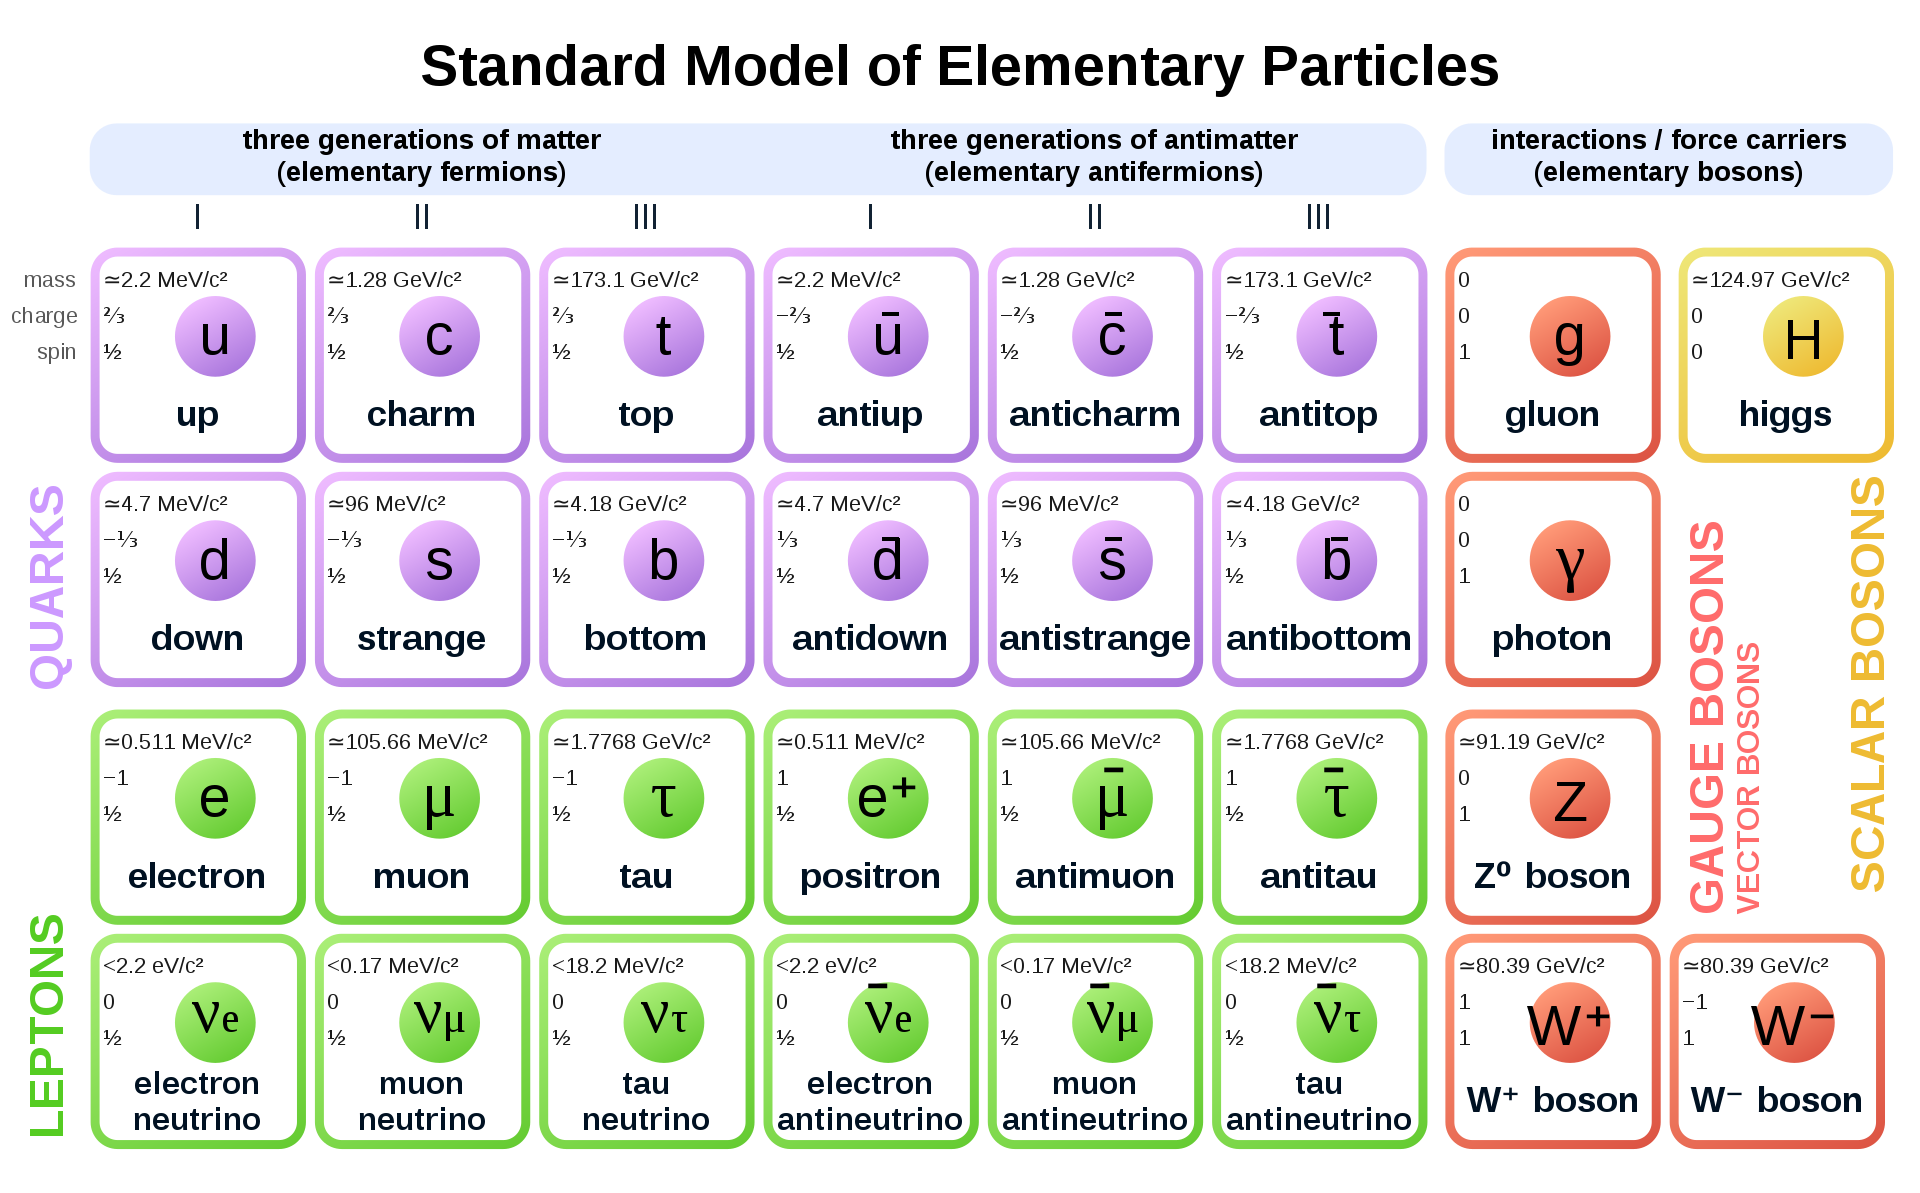
\includegraphics[width=1\textwidth]{figs/ch2/standard_model}
\caption{The Standard Model of Particle Physics. This displays all three generations of fermions 
in purple and green along with their antiparticle. On the right in red shows the force carrying
bosons along with the Higgs boson shown in yellow. Corresponding table of values can be 
found in Table \ref*{table:sm} on page \pageref*{table:sm}. }
\label{fig:sm_fig}
\end{figure}

\subsection{Theoretical Foundation}

The \gls{sm} represents a gauge theory that describes the strong, weak and electromagnetic interactions  
The \gls{sm} Lagrangian $\Lagr_{SM}$ can be broken down into two Lagrangians representing the strong interaction $\Lagr_{QCD}$
and the electroweak (\gls{ew})interaction $\Lagr_{EW}$. As in the name, the \gls{ew} theory is the combination of the electromagnetic 
and weak interactions. The Lagrangian $\Lagr_{SM}$ is invariant under local gauge transformations with the symmetry groups \cite{pich}.

\begin{equation}\label{eq:2.1} 
    \underbrace{SU(3)_{C}}_\text{QCD} \otimes \underbrace{SU(2)_{L} \otimes U(1)_{Y}}_\text{electroweak}
\tag{2.1}
\end{equation}
\\
The interactions between the strong, weak and electromagnetic forces are through the exchange of spin-1 gauge fields. For the strong field;
8 massless gluons. For the weak; 3 massive bosons, $W^\pm$ and $Z^0$. For the electromagnetic;
1 massless photon. The fermionic particles in Table \ref{table:sm} and Figure \ref{fig:sm_fig} can be represented
in a 3-fold family structure:
\\
\begin{equation}\label{eq:2.2}
  \begin{bmatrix}
    \nu_{e} & \textit{u} \\ 
    e^- & \textit{d}'
  \end{bmatrix}    
  ,
  \qquad
  \begin{bmatrix}
    \nu_{\mu} & \textit{c} \\
    \mu^- & \textit{s}'
  \end{bmatrix}
  ,
  \qquad
  \begin{bmatrix}
    \nu_{\tau} & \textit{t} \\
    \tau^- & \textit{b}'
  \end{bmatrix}
\tag{2.2}
\end{equation}
\\
where each quark appears in three different colors:
\\
\begin{equation}\label{eq:2.3}
    \begin{bmatrix}
        \nu_{\textit{l}} & \textit{q}_{u} \\
        \textit{l}^- & \textit{q}_{d}
    \end{bmatrix}
    \quad
    \equiv
    \quad 
    \begin{pmatrix}
        \nu_{\textit{l}} \\
        \textit{l}^-
    \end{pmatrix}_{L}
    ,
    \quad
    \begin{pmatrix}
        q_{\textit{u}} \\ 
        q_{\textit{d}} 
    \end{pmatrix}_{L}
    ,
    \quad
   l_{R}^-,\ q_{\textit{u}R},\ q_{\textit{d}R}
\tag{2.3}
\end{equation}
\\
plus their corresponding antiparticles. Here we see that the left-handed fields are 
$SU(2)_{L}$ doublets, whereas the right-handed partners transform as $SU(2)_{L}$ singlets.
 \par
 The vacuum-induced breakdown of gauge symmetry initiates Spontaneous Symmetry Breaking (\gls{ssb}) 
(as discussed later in section 2.2.3) within the \gls{ew} group, resulting in the emergence of the electromagnetic subgroup.
\\
 \begin{equation}\label{eq:2.4} 
    SU(3)_{C} \otimes SU(2)_{L} \otimes U(1)_{Y} \qquad \overrightarrow{\gls{ssb}} \qquad SU(3)_{C} \otimes U(1)_{QED} 
\tag{2.4}
\end{equation}
\\
The \gls{ssb} mechanism is the cause of the masses of the weak gauge bosons ($W^\pm$,$Z^0$) and gives rise 
to the appearance of a physical scalar boson in the \gls{sm} which can be seen as the yellow "Higgs" in 
Figure \ref{fig:sm_fig}. This also gives rise to the fermion masses and their mixings. These mixings keep track
of weak decays, i.e. one quark transitioning to another quark. These mixings were first formulated into 
a 6-quark model by Kobayashi and Maskawa by generalizing the Cabibbo matrix, creating the Cabibbo-Kobayashi-Maskawa (\gls{ckm}) matrix.
This matrix keeps track of weak decay rates in three generations of quarks \cite{ckm}.
\\
\begin{equation}\label{eq:2.5}
    \begin{bmatrix}
        d' \\
        s' \\
        b'
    \end{bmatrix}
    \quad
    =
    \quad
    \begin{bmatrix}
        V_{ud} & V_{us} & V_{ub} \\
        V_{cd} & V_{cs} & V_{cb} \\
        V_{td} & V_{ts} & V_{tb} \\
    \end{bmatrix}
    \begin{bmatrix}
        d \\
        s \\
        b \\
    \end{bmatrix}
\end{equation}
\\
Here we see on the left side are the weak interaction doublet partners of down-type quarks. On
the right side is the \gls{ckm} matrix along with a vector of mass eigenstates of down-type quarks.
The \gls{ckm} matrix states the probability of transitions between one quark flavor \textit{j} to another quark flavor \textit{i}.
These transitions are proportional to $|V_{ij}|^2$. 
\\
\begin{equation}\label{eq:2.6}
    \medmath{
    \begin{bmatrix}
        |V_{ud}| & |V_{us}| & |V_{ub}| \\
        |V_{cd}| & |V_{cs}| & |V_{cb}| \\
        |V_{td}| & |V_{ts}| & |V_{tb}| 
    \end{bmatrix}
    =
    \begin{bmatrix}
       0.97373 \pm 0.00031 & 0.2243 \pm 0.0008 & 0.00382 \pm 0.00020 \\
       0.221 \pm 0.004 & 0.975 \pm 0.006 & 0.0408 \pm 0.0014 \\
       0.0086 \pm 0.0002 & 0.0415 \pm 0.0009 & 1.014 \pm 0.029 \\ 
    \end{bmatrix}
    }
\tag{2.6}
\end{equation}
\\
Here we see in Eq. \ref{eq:2.6} the most recent transition probabilities as stated 
by the Particle Data Group (\gls{pdg}) \cite{workman}. Now, we expect unitary of the \gls{ckm} 
matrix but if we check it, even in the first row, we see:
\\
\begin{equation}\label{eq:2.7}
    |V_{ud}|^2 \ + |V_{us}|^2 \ + |V_{ub}|^2 \ = \ 0.9985 \pm 0.0007
\tag{2.7}
\end{equation}
\\
The difference from the theoretical unitary value of 1 has a standard deviation of 2.2$\sigma$ which 
this gives an exciting strong indication of physics Beyond the Standard Model or \gls{bsm}. 
\\
\subsection{Fundamental Interactions}
\subsubsection{The Electromagnetic Interaction}

Quantum Electrodynamics (\gls{qed}) is the foundational knowledge of electromagnetism. All charged particles
communicate with each other through the electromagnetic force carrier boson called the Photon. \gls{qed} is a 
consequence of the $U(1)$ symmetry. It is the separated force from the \gls{ew} interactions and can be seen 
in Eq. \ref{eq:2.1} as $U(1)_{em}$. In order to obtain the \gls{qed} Lagrangian, let's look at the dynamics of
a free $1/2$ spin fermion.
%
\begin{equation}\label{eq:2.8}
    \Lagr_{0} = \bar{\psi}(i\gamma^{\mu}-m)\psi
\tag{2.8}
\end{equation}
%
In Eq. \ref{eq:2.8} notation-wise, $\psi$ is the Dirac Spinor, $m$ is the mass and the Dirac matrices are 
denoted by $\gamma^{\mu} \cdot \bar{\psi} = \psi^{\dag} \; \gamma^{0}$ which is also known as the Dirac adjoint.
In the Lagrangian, the $\gamma^{\mu}$ are the Dirac $4 \ \times \ 4$ matrices and can be seen in Eq. \ref{eq:2.9}.
%
\begin{equation}\label{eq:2.9}
    \gamma^{0}=
    \begin{bmatrix}
        0 \ \ & I \\
        -I \ \ & 0 \\
    \end{bmatrix}
    ,
    \quad
    \gamma^{i}=
    \begin{bmatrix}
        0  & \sigma^{i} \\
        -\sigma^{i} & 0 \\
    \end{bmatrix}
    ,
    \quad
    \gamma^{5}=
    \begin{bmatrix}
        -I \ \ & 0 \\
        0 \ \ & I \\
    \end{bmatrix}
\tag{2.9}    
\end{equation}
%
These are written in terms of the Pauli matrices which are shown in Eq. \ref{eq:2.10}.
%
\begin{equation}\label{eq:2.10}
    \sigma^{1}=
    \begin{bmatrix}
       \ 0 \ \ \  \ & 1 \ \\
       \ 1 \ \ \  \ & 0 \ \\
    \end{bmatrix}
    ,
    \quad
    \sigma^{2}=
    \begin{bmatrix}
        0  \ \  & i \ \\
        -i \ \  & 0 \ \\
    \end{bmatrix}
    ,
    \quad
    \sigma^{3}=
    \begin{bmatrix}
       \ 1 \  \ & 0 \ \\
       \ 0 \  \ & -1 \ \\
    \end{bmatrix}
\tag{2.10}
\end{equation}
%
The Lagrangian in Eq. \ref{eq:2.8} is invariant under global gauge transformations, but is 
not invariant under local $U(1)$ transformations. In order to induce local invariance under transformations,
as shown in Eq. \ref{eq:2.11}, an additional vectorial gauge field that is massless is required.
%
\begin{equation}\label{eq:2.11}
    \psi(x) \rightarrow \psi'(x) = e^{i\alpha(x)}\psi(x)  
\tag{2.11}
\end{equation}
%
The gauge field that is required is denoted as $A_{\mu}(x)$ and is shown in eq \ref{eq:2.12}.
Additionally, the covariant derivative $D_{\mu}(x)$ is shown in Eq. \ref{eq:2.13}.
%
\begin{equation}\label{eq:2.12}
    A_{\mu}(x) \rightarrow A_{\mu}'(x) = A_{\mu}(x) \ + \ \frac{1}e\partial_{\mu}\alpha(x)
\tag{2.12}    
\end{equation}
%
\begin{equation}\label{eq:2.13}
    D_{mu}(x) = \partial_{mu} \ - \ ieA_{\mu}(x)
\tag{2.13}
\end{equation}
%
Using these two fields, the field strength tensor can be expressed in Eq. \ref{eq:2.14}.
%
\begin{equation}\label{eq:2.14}
    F_{\mu\nu} = \partial_{\mu}A_{\nu} \ - \ \partial_{\nu}A_{\mu}
\tag{2.14} 
\end{equation}
%
Now that local $U(1)$ symmetry is applied, Eq. \ref{eq:2.11} can be used along with Eq. \ref{eq:2.14}
to express the \gls{qed} Lagrangian. This is shown in Eq. \ref{eq:2.15}.
%
\begin{equation}\label{eq:2.15}
    \Lagr = \bar{\psi}i\gamma^{\mu}-m)\psi \ - \ \frac{1}4F_{\mu\nu}F^{\mu\nu}
\tag{2.15}
\end{equation}
%
From here, the interaction term called the electromagnetic charge current density $j^{\mu}$
is added to Eq. \ref{eq:2.15}. This equation is defined in Eq. \ref{eq:2.16}. 
%
\begin{equation}\label{eq:2.16}
    j^{\mu} = \bar{\psi}\gamma^{\mu}\psi
\tag{2.16}
\end{equation}
%
putting both of these equations together we get Eq. \ref{eq:2.17}.
%
\begin{equation}\label{eq:2.17}
    \Lagr = \underbrace{\bar{\psi}i\gamma^{\mu}-m)\psi}_\text{free Lagrangian} \ \ \ -  \underbrace{ej^{\mu}A_{\mu}}_\text{interaction term}  - \ \ \ \underbrace{\frac{1}4F_{\mu\nu}F^{\mu\nu}}_\text{kinetic term}
\tag{2.17}
\end{equation}
%
Here, Eq. \ref{eq:2.17} is the \gls{qed} Lagrangian. According to Noether's theorem which states 
that every differentiable symmetry of the action of a physical system with conservative forces has
a corresponding conservation law \cite{noether}. For QED, this conserved quantity is the electromagnetic 
charge \textit{q}. The \gls{qed} Lagrangian thus shows the relationship between the photon field $A_{\mu}$ 
and the Dirac fields $\psi$ which emerged as a consequence of $U(1)$ symmetry.
%

\subsubsection{The Electroweak Interaction}

The \gls{ew} force is the combination of the electromagnetic interaction and the weak interaction.
Both of these forces appear differently in low energies but they happen to combine at much higher
energies. Thus, this theory models them as two different aspects of the same force. The predicted 
unification energy is on the order of 246 Gev or on a temperature scale of approximately $10^{15} K$. 
This implies that the two forces coexisted at the start of the Big Bang and later diverged during 
the Quark Epoch, occurring approximately $10^{-12}$ seconds after the inception of the Big Bang.
\par
The mathematical formulation is found within the $SU(2)_{L}$ symmetry group in Eq. \ref{eq:2.1}. 
Weak isospin and weak hypercharge are quantum numbers relating the electrically charged part of the weak interaction and are 
labeled $T_{\textit{i}}$ and $Y_{W}$ respectively. These are known as generators of $SU(2)$ and $U(1)$ and give rise to the gauge
bosons that mediate this force. Once \gls{ssb} occurs, these bosons are seen in the \gls{sm} as the $W^{\pm}$, 
$Z^{0}$, and the photon. The conserved quantity within the electroweak force is the third component of the generator 
$T_{\textit{i}}$, quantum number $T_{3}$. However, interaction with the Higgs field do not conserve weak isospin $T_{3}$
and thus causing fermion mixings as seen in the \gls{ckm} matrix in \ref{eq:2.6}. Though, there are specific combinations
of them that do not interact with the Higgs field and therefore are conserved, this happens to be the electric charge \textit{q}.
The combinations that give rise to \textit{q} are given by Eq. \ref{eq:2.18}.
%
\begin{equation}\label{eq:2.18}
    Q = T_{3} + \frac{1}2Y_{W}
\tag{2.18}
\end{equation}
%
The \gls{ew} force is \textit{chiral}, which requires treating both components of the fermionic fields $\psi$ separately.
Left-handed fermions have weak isospin of $T_{3}=\pm 1/2$ and are represented by doublets $\psi_{L}$. Whereas right-handed
fermions have weak isospin of $T_{3} = 0$ and are represented by singlets $\psi_{R}$. Both components behave differently under
$SU(2)_{L}$ and $U(1)_{\gamma}$ local transformations. A quick formulation of the \gls{ew} Lagrangian can be formulated
by introducing the covariant derivative acting on both the left-handed fermionic field (Eq. \ref{eq:2.19}) and the right-handed
fermionic field (Eq. \ref{eq:2.20}).
%
\begin{equation}\label{eq:2.19}
    D_{\mu}\psi_{L}=(\partial_{\mu} \ + \ ig\frac{\sigma_{i}}2W_{\mu}^{i} \ + \ ig'\frac{\gamma}2B_{\mu}^{i})\psi_{L}
\tag{2.19}
\end{equation}
%
\begin{equation}\label{eq:2.20}
    D_{\mu}\psi_{R}=(\partial_{\mu} \ + \  ig'\frac{\gamma}2B_{\mu}^{i})\psi_{R}
\tag{2.20}
\end{equation}
%
Here we see the Pauli matrices $\sigma$ that are shown in Eq. \ref{eq:2.10}, $g$ and $g'$ are coupling constants for 
the $W^{i}$ and $B_{\mu}$ boson field strength tensors which are shown in Eq. \ref{eq:2.21} and Eq. \ref{eq:2.22}.
%
\begin{equation}\label{eq:2.21}
    B_{\mu\nu} = \partial_{\mu}B_{\nu} \ - \ \partial_{\nu}B_{\mu}
\tag{2.21}
\end{equation}
%
\begin{equation}\label{eq:2.22}
    W^{i}_{\mu\nu} = \partial_{\mu}W^{\nu}_{i} \ - \ \partial_{\nu}W^{\mu}_{i} \ - \ \epsilon_{ijk} W^{\mu}_{j}G^{\nu}_{k}
\tag{2.22}
\end{equation}
%
With these, the electroweak Lagrangian can be assembled as shown in Eq. \ref{eq:2.23} where the sum over $j$ covers the $L$
doublet and two $R$ singlets.
%
\begin{equation}\label{eq:2.23}
    \Lagr_{EW} =  \sum_{j=1}^{3}\bar{\psi_{j}}[i\gamma^{\mu}D_{\mu}]\psi_{j} \ - \ \frac{1}4W_{i}^{\mu\nu}W_{\mu\nu}^{i} \ - \ \frac{1}4B^{\mu\nu}B_{\mu\nu}  
\tag{2.23}
\end{equation}
%
Both, $W^{\pm}$ bosons arise from linear combinations between $W_{1}$ and $W_{2}$ as shown in Eq. \ref{eq:2.24}.
%
\begin{equation}\label{eq:2.24}
    W^{\pm} = \frac{1}{\sqrt{2}}(W_{1} \mp iW_{2})
\tag{2.24}
\end{equation}
%
Finally, the application of a rotation by an angle $\theta_{W}$ allows the restoration of the massless vector field $A$ that's 
associated with the photon and the massive weak neutral $Z^{0}$. Here, $\theta_{W}$ represents the \textit{weak mixing angle}. This 
rotation introduces the mismatch between the $W^{\pm}$ bosons and the $Z^{0}$ boson. Through \gls{ssb}, the two bosons (photon and $Z^{0}$)
become physical with different masses given by Eq. \ref{eq:2.25}.
%
\begin{equation}\label{eq:2.25}
    \begin{pmatrix}
        \gamma \\
        Z^{0} \\
    \end{pmatrix}
    =
    \begin{pmatrix}
        cos\theta_{W} & sin\theta_{W} \\ 
        -sin\theta_{W} & cos\theta_{W} \\
    \end{pmatrix}
    \begin{pmatrix}
        B \\
        W_{3} \\
    \end{pmatrix}
\tag{2.25}
\end{equation}
%
where the offset of the $Z^{0}$ mass from the $W^{\pm}$ bosons can be given by Eq. \ref{eq:2.26}.
%
\begin{equation}\label{eq:2.26}
    m_{Z} = \frac{m_{W}}{cos\theta_{W}}
\tag{2.26}
\end{equation}
%
A pictorial representation of this \textit{weak mixing angle} showing the pattern of weak 
isospin, $T_{3}$, and weak hypercharge, $Y_{W}$, of the known elementary particles can be seen 
in Figure \ref{fig:wma}. 
%
\newpage
\begin{figure}[ht]
    \centering
    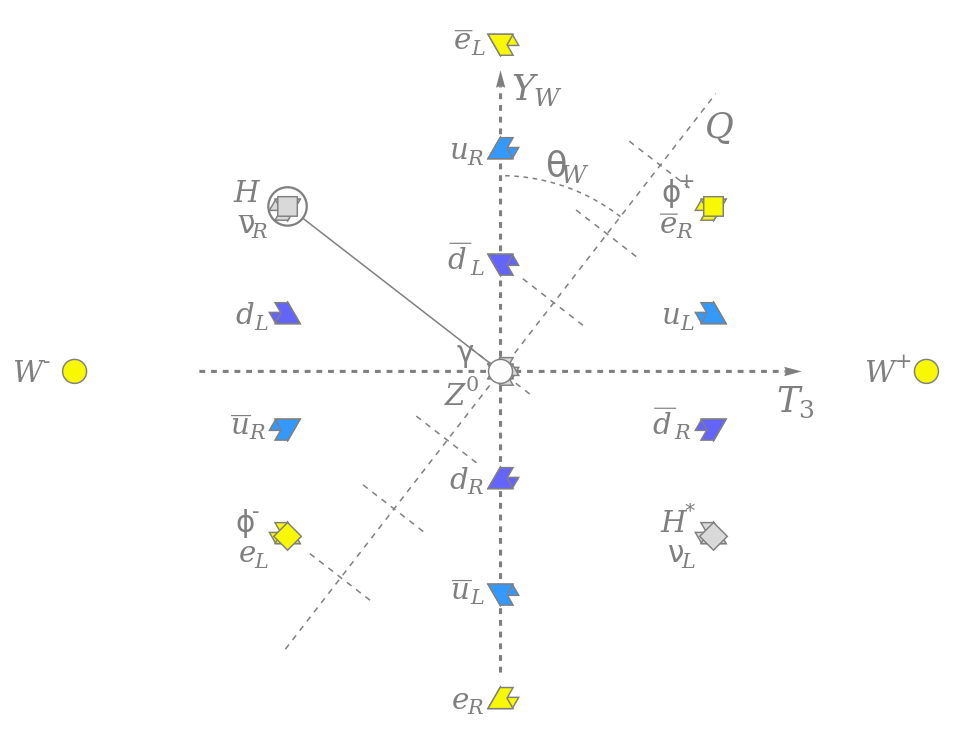
\includegraphics[scale=0.55]{figs/ch2/weak_mixing_angle}%width=14cm, height=14cm
    \caption{ The pattern of weak isospin, $T_{3}$, and weak hypercharge, $Y_{W}$, of the known elementary particles.
    The electric charge is shown as $Q$ along the \textit{weak mixing angle}. The neutral Higgs field is seen being
    circled, this field breaks the electroweak symmetry and interacts with other particles, giving them mass. }
\label{fig:wma}
\end{figure}


\subsubsection{The Strong Interaction}

The strong interaction, or the strong force, is the fundamental force that confines quarks, forming hadrons.
It is also the reason why nuclei are able to bind inside the nucleus forming atomic nuclei. 
To model the strong interaction, Quantum Chromodynamics, i.e. \gls{qcd}, is used. This theory was founded on 
Yang-Mills theory \cite{yang-mills}, which extends \gls{qed}, adding the non-abelian symmetry group $SU(3)$. 
Quarks interact with gluons and each other by way of a type of charge called the color charge. Unlike the 
electromagnetic charge, color charges comes with three types ($\pm$red, $\pm$green, $\pm$blue) which dictates
the rules of behavior. Due to the strength of this force, when hadrons collide with high energy particles, jets of massive particles are produced instead of emitting their constituents as separate particles. 
\par
In the symmetry group $SU(3)$ Lie algebra, there are eight generators, therefore just as many gauge fields need to 
be introduced. The associated fermionic fields are represented by three-dimensional vectors, i.e. triplets, where 
each component represents color charges. Matrices called the Gell-Mann matrices $t_{a}$ are used to represent 
the generators, having the commutation relationship: $[t_{a},t_{b}]=if_{abc}t_{c}$.
Under a transformation $U(x)$, the quark field $\psi$ behaves as stated in Eq. \ref{eq:2.27}.
%
\begin{equation}\label{eq:2.27}
    \psi(x) \rightarrow \psi'(x) = U(x)\psi = e^{i\alpha_{a}(x)t_{a}}\psi
\tag{2.27}    
\end{equation}
% 
Similarly to the \gls{qed}'s case, new fields are introduced: the gluon field $G^{a}_{\mu}$ and 
a covariant derivative, as seen in Eq. \ref{eq:2.28}.
%
\begin{equation}\label{eq:2.28}
    D_{\mu} = \partial_{\mu} + ig_{s}t_{a}G^{a}_{\mu}
\tag{2.28}
\end{equation}
%
The gluon field behavior has requirements under the transformation $U(x)$. These 
requirements are shown in Eq. \ref{eq:2.29}.
%
\begin{equation}\label{eq:2.29}
    G^{a}_{\mu} \rightarrow G'^{a}_{\mu} = U(x)G^{a}_{\mu}t^{a}U^{\dagger}(x) + \frac{i}g_{s}(d_{\mu}U(x))U^{\dagger}(x)
\tag{2.29}
\end{equation}
%
The field strength tensor for the gluon field $G^a_{\mu}$ that follows the requirements as stated 
in Eq. \ref{eq:2.29} is shown in Eq. \ref{eq:2.30}.
%
\begin{equation}\label{eq:2.30}
    G^{\mu\nu}_{a} = \partial_{\mu}G^{\nu}_{a} - \partial_{\nu}G^{\mu}_{a} - g_{s}f_{abc}G^{\mu}_{b}G^{\nu}_{c}
\tag{2.30}
\end{equation}
%
Lastly, the \gls{qcd} Lagrangian density, using the previously shown equations, can be derived 
and is shown in Eq. \ref{eq:2.31}.
%
\begin{equation}\label{eq:2.31}
    \Lagr_{QCD} = \bar{\psi}(i\gamma^{\mu}D_{\mu} - m)\psi - \frac{1}4G^{\mu\nu}_{a}G^{a}_{\mu\nu}
\tag{2.31}
\end{equation}
%
Here, we see a noteworthy aspect of the \gls{qcd} Lagrangian which is the self interaction between 
gluons due to having color charge. 

\subsection{Spontaneous Symmetry Breaking}

The gauge symmetries of the \gls{sm} ($SU(3)_{C}$, $SU(2)_{L}$, $SU(1)_{\gamma}$) have proven to 
be successful in predicting interactions between its particles. But particles have masses (besides the photon)!
So far, there has been no references to any mass terms within these symmetries. Another mechanism 
was needed in order to allow generation of masses within these gauge theories. This mechanism is called 
spontaneous symmetry breaking (\gls{ssb}).
\par
Suppose there is a scalar field $\phi$ with a corresponding Lagrangian.
%
\begin{equation}\label{eq:2.32}
    \Lagr = \frac{1}2(\partial_{\mu}\phi)(\partial^{\mu}\phi)+e^{-(\alpha\phi)^{2}}
\tag{2.32}
\end{equation}
%
There is no obvious mass term within this Lagrangian, but if the exponential is expanded, we get:
%
\begin{equation}\label{eq:2.33}
    \Lagr = \frac{1}2(\partial_{\mu}\phi)(\partial^{\mu}\phi)+1-\alpha^{2}\phi^{2}+\frac{1}2\alpha^{4}\phi^{4}-\frac{1}6\alpha^{6}\phi^{6}+ \ ...
\tag{2.33}
\end{equation}
%
Here, the 1 is irrelevant, but the second term is close to the known mass term within the Klein-Gordon equation, with $\alpha^{2} = \frac{1}2(mc/\hbar)^{2}$, while the higher 
order terms correspond to coupling terms. The Lagrangian describes a particle of mass: 
%
\begin{equation}\label{eq:2.34}
    m=\sqrt{2}\alpha\hbar/c
\tag{2.34}
\end{equation}
%
Now that the hidden mass term can be found within a Lagrangian for a field, suppose there's a Lagrangian 
that takes the form: 
%
\begin{equation}\label{eq:2.35}
    \Lagr = \frac{1}2(\partial_{\mu}\phi)(\partial^{\mu}\phi)+\frac{1}2\mu^{2}\phi^{2}-\frac{1}4\lambda^{2}\phi^{4}
\tag{2.35}
\end{equation}
%
Here the second term looks like the mass term as previously discussed be we see that the sign is flipped and 
therefore would be imaginary. In order to properly understand this, Feynman calculus must be used which 
treats this more like a perturbation procedure which is started from the ground state, or vacuum. We must represent this 
Lagrangian classically, as seen in \ref{eq:2.36}, in order to obtain the minimum.
%
\begin{equation}\label{eq:2.36}
    \Lagr = \textit{T} - \textit{U}
\tag{2.36}
\end{equation}
%
We obtain the minimum:
%
\begin{equation}\label{eq:2.37}
    \textit{U}(\phi) = -\frac{1}2\mu^{2}\phi^{2}+\frac{1}4\lambda^{2}\phi^{4}
\tag{2.37}
\end{equation}
%
We see that the minimum occurs at:
%
\begin{equation}\label{eq:2.38}
    \phi = \pm\mu/\lambda
\tag{2.38}
\end{equation}
%
A new variable, $\eta$, must be introduced which represents a perturbation around this ground state.
%
\begin{equation}\label{eq:2.39}
    \eta \equiv \phi \pm \frac{\mu}\lambda
\tag{2.39}
\end{equation}
%
Now, to rewrite the Lagrangian in Eq. \ref{eq:2.35} in terms of $\eta$.
%
\begin{equation}\label{eq:2.40}
    \Lagr = \frac{1}2(\partial_{\mu}\eta)(\partial^{\mu}\eta)-\mu^{2}\eta^{2}\pm\mu\lambda\eta^{3}-\frac{1}4\lambda^{2}\eta^{4} + \frac{1}4(\mu^{2}/\lambda)^{2}
\tag{2.40}
\end{equation}
%
The second term is now the correct sign for the mass term! The mass of the particle from the Lagrangian is:
%
\begin{equation}\label{eq:2.41}
    m = \sqrt{2}\mu\hbar/c
\tag{2.41}
\end{equation}
%
Where the third and fourth term are corresponding coupling terms. Figure \ref{fig:2d_potential} shows 
the shape of the potential $U(\phi)$ and its minima. 
%
\begin{figure}[h]
    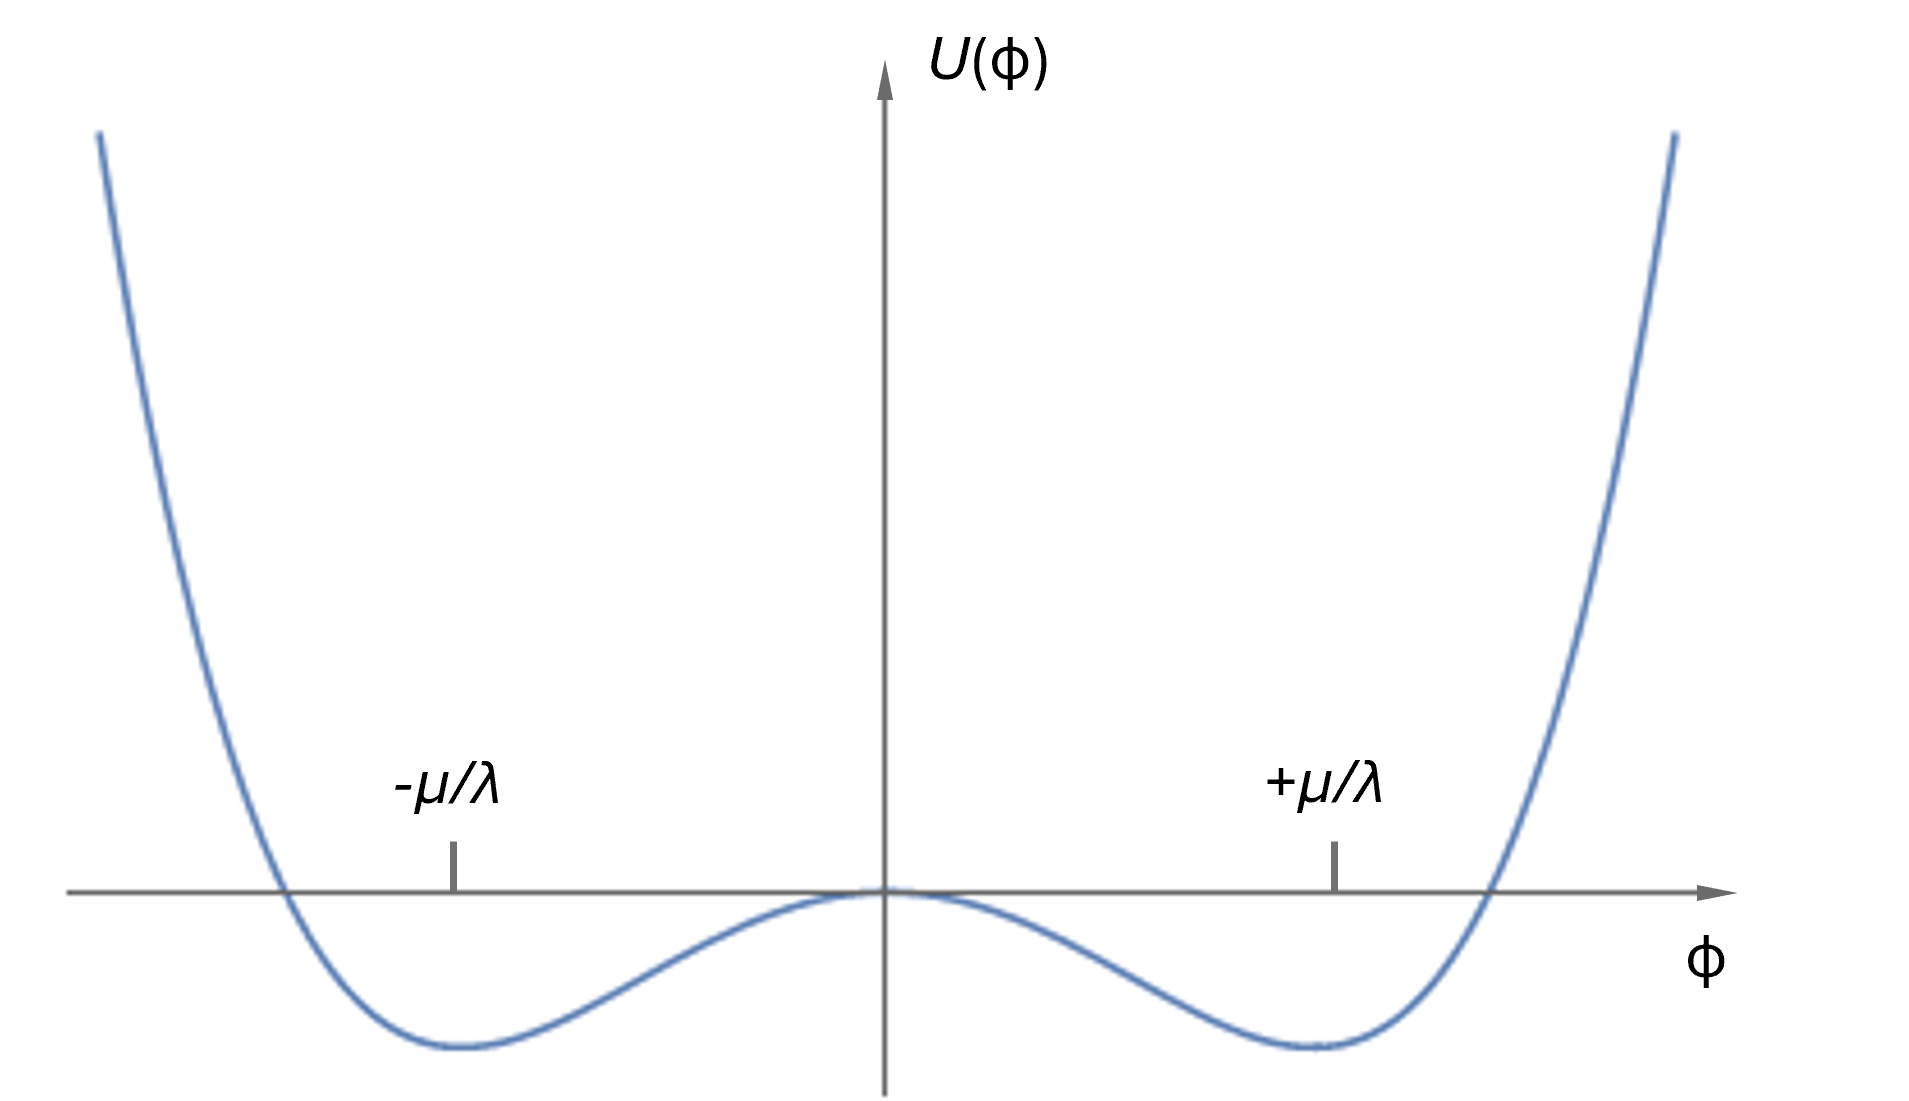
\includegraphics[width=0.8\linewidth,height=8cm]{figs/ch2/2d_potential.png}
    \centering
\caption{Graph of $\textit{U}(\phi)$ in Eq. \ref{eq:2.37}}
\label{fig:2d_potential}
\end{figure}
 %   
This example illustrates \gls{ssb}, though it may not be too obvious. The Lagrangian in Eq. \ref{eq:2.40}
is the same as Eq. \ref{eq:2.35} except for one thing, its symmetry is broken. The Lagrangian in 
Eq. \ref{eq:2.35} is \textit{even} in $\phi$, as in, it's invariant ($\phi \rightarrow -\phi$).
Whereas the Lagrangian in \ref{eq:2.40} is not, thus \gls{ssb}. This happens due to the fact that the chosen state,
i.e. the ground state, does not share this symmetry. However, the collection of all states does share this 
symmetry. This example shows a broken \textit{discrete} symmetry, i.e left or the right side in Figure \ref{fig:2d_potential}.
To make this more physical, let's consider a Lagrangian containing continuous symmetries that demonstrates \gls{ssb}. 
%
\begin{equation}\label{eq:2.42}
    \Lagr = \frac{1}2(\partial_{\mu}\phi_{1})(\partial^{\mu}\phi_{1}) + \frac{1}2(\partial_{\mu}\phi_{2})(\partial^{\mu}\phi_{2}) + \frac{1}2\mu^{2}(\phi^{2}_{1}+\phi^{2}_{2})-\frac{1}4\lambda^{2}(\phi^{2}_{1}+\phi^{2}_{2})^{2}
\tag{2.42}
\end{equation}
%
Now this has two fields, $\phi_{1}$ and $\phi_{2}$, and only contains sum of squares, therefore it is invariant under
\textit{rotations} in $\phi_{1}$, $\phi_{2}$ space. The potential $U(\phi_{1},\phi_{2})$ is then:
%
\begin{equation}\label{eq:2.43}
    \textit{U}(\phi_{1},\phi_{2}) = -\frac{1}2\mu^{2}(\phi^2_{1}+\phi^2_{2})+\frac{1}4\lambda^{2}(\phi^{2}_{1}+\phi^{2}_{2})^{2}
\tag{2.43}
\end{equation}
%
and the minima lie on the circle of radius $\mu/\lambda$:
%
\begin{equation}\label{eq:2.44}
    \phi^{2}_{1}+\phi^{2}_{2} = \mu^{2}/\lambda^{2}
\tag{2.44}
\end{equation}
%
Now in order to apply Feynman calculus as we did previously, we must expand around a particular ground state or vacuum.
%
\begin{equation}\label{eq:2.45}
    \phi_{1} = \mu/\lambda: \\ \phi_{2} = 0
\tag{2.45}
\end{equation}
%
\begin{figure}[h]
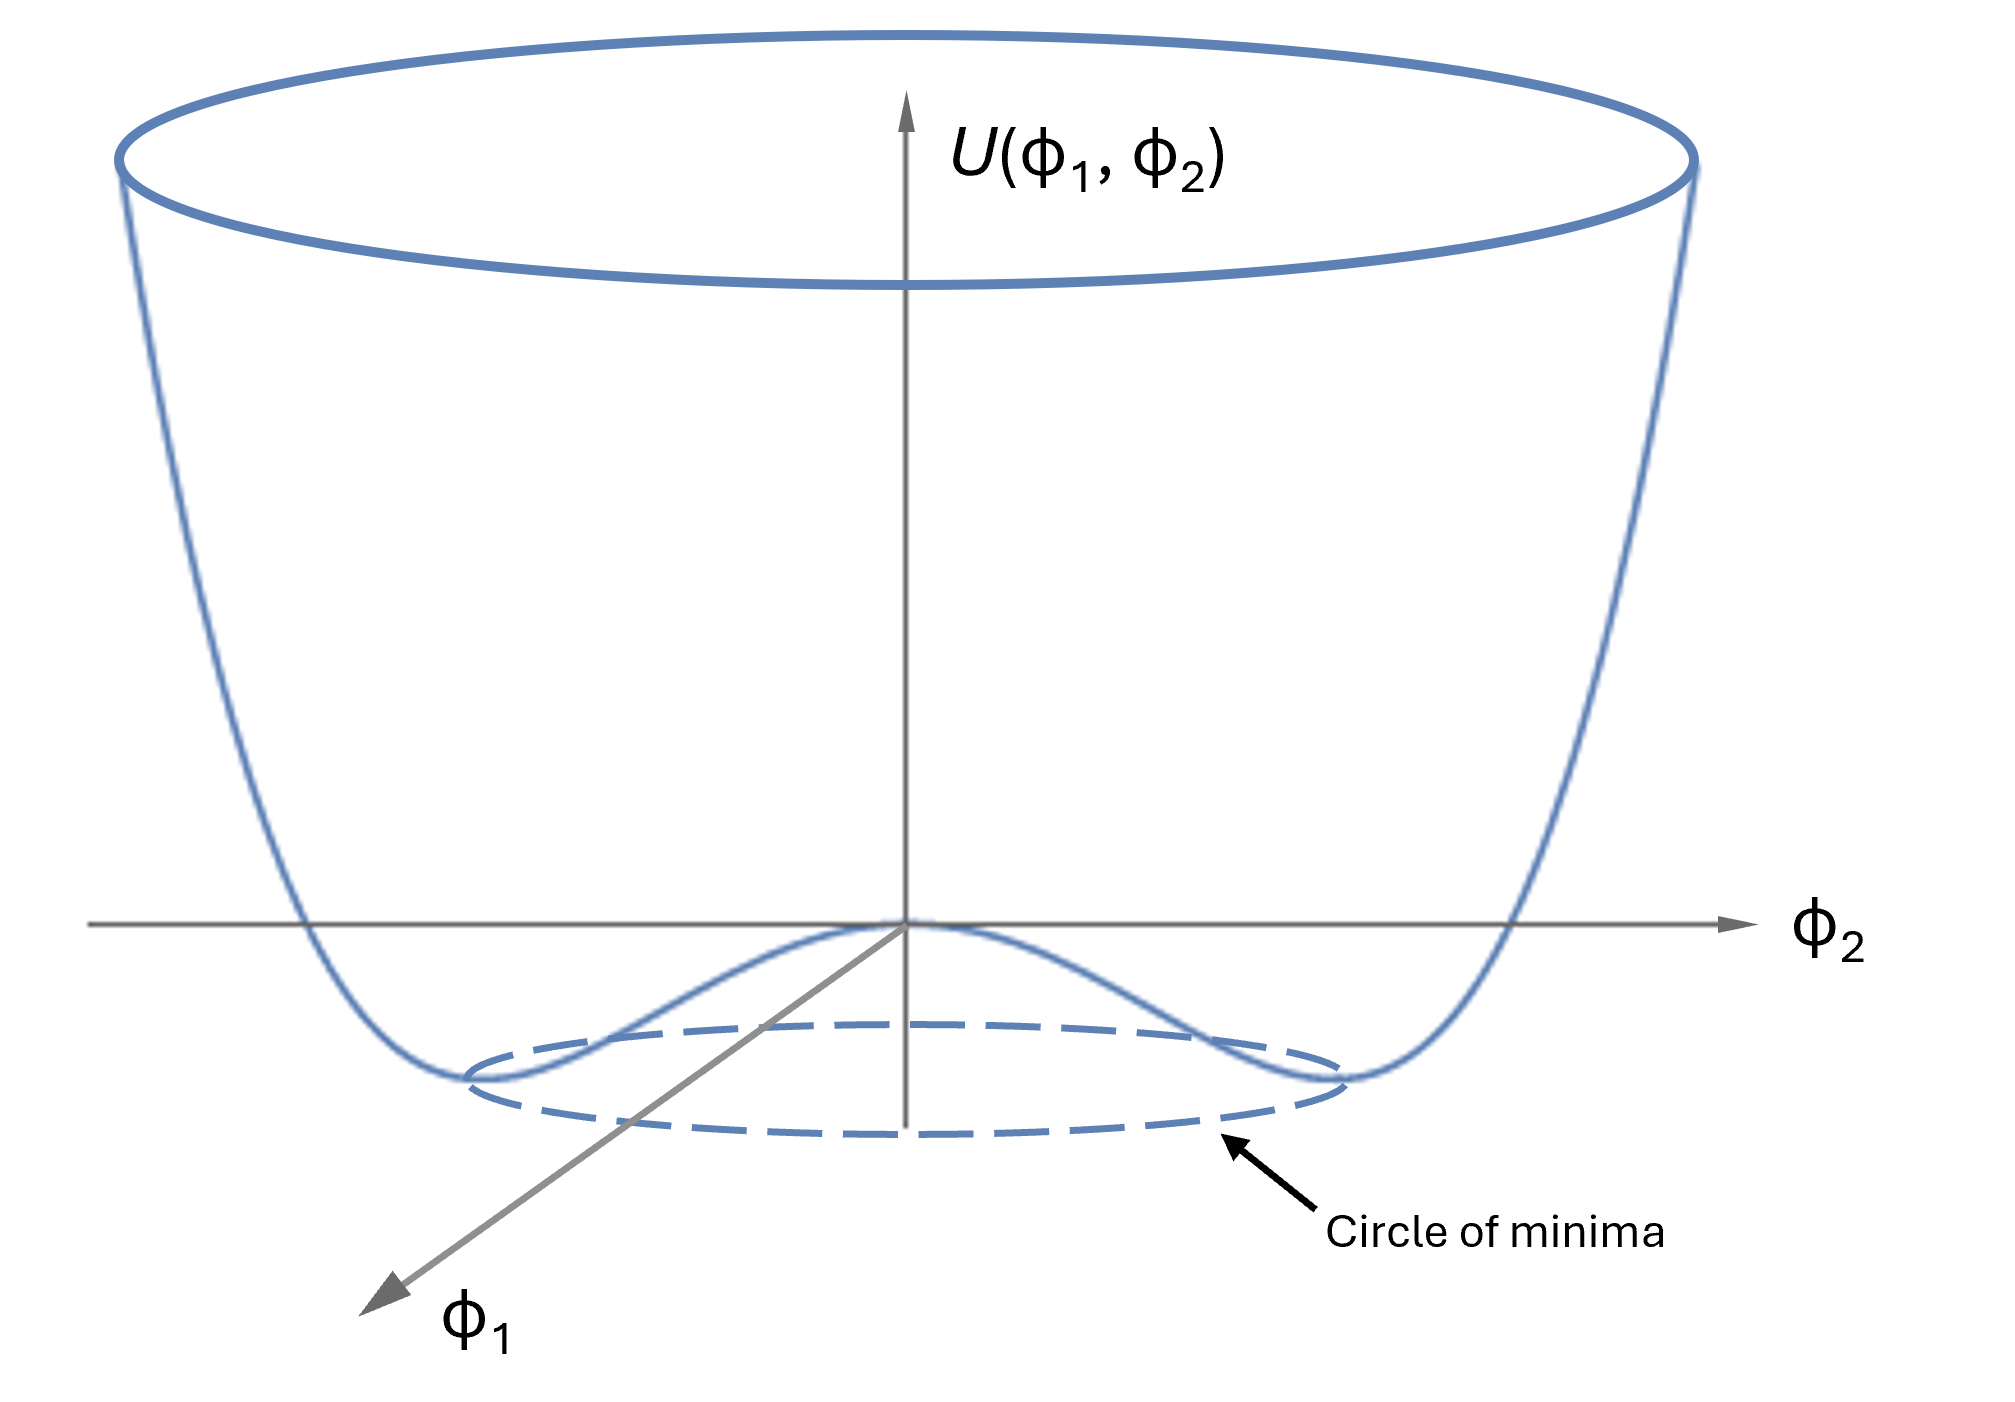
\includegraphics[width=0.8\linewidth,height=8cm]{figs/ch2/3d_pot_graph2.png}
\centering
\caption{Graph of $\textit{U}(\phi_{1},\phi_{2})$ in Eq. \ref{eq:2.43}}
\label{fig:3d_pot_graph2}
\end{figure}
%
Following the steps shown above, we introduce new fields that represent fluctuations around the vacuum.
%
\begin{equation}\label{eq:2.46}
    \eta \equiv \phi_{1}-\mu/\lambda; \qquad \nu \equiv \phi_{2}
\tag{2.46}
\end{equation}
%
Rewriting the Lagrangian from Eq. \ref{eq:2.42} using these new fields:
%
\begin{equation}\label{eq:2.47}
\begin{split}
    \Lagr = &[\frac{1}2(\partial_{\mu}\eta\partial^{\mu}\eta)  - \mu^{2}\eta^{2}] + [\frac{1}2(\partial_{\mu}\nu\partial^{\mu}\nu)] \ - \ \\  
    &[\mu\lambda(\eta^{3} + \eta\nu^{2}) + \frac{\lambda^{2}}4(\eta^{4}+\nu^{4}+2\eta^{2}\nu^{2})] + \frac{\mu^{4}}{4\lambda^{2}}
\end{split}
\tag{2.47}
\end{equation}
%
The first term is the free Klein-Gordon Lagrangian for the field $\eta$, carrying a mass of:
%$\qquad \qquad \qquad \qquad \qquad \qquad \qquad \quad \ \ \ $
\begin{equation}\label{eq:2.48}
    m_{\eta} = \sqrt{2}\mu\hbar/c
\tag{2.48}
\end{equation}
%
The second term is a free Lagrangian for the field $\nu$, which is massless:
%
\begin{equation}\label{eq:2.49}
    m_{\nu} = 0
\tag{2.49}
\end{equation}
%
The third and fourth term show five different couplings. An important phenomena that occurs here is that 
one of the two fields is \textit{massless}. This is to be expect since \gls{ssb} of a continuous symmetry 
is always accompanied by one or more massless scalar (spin-0) particles, these are called Goldstone Bosons.
At first glance this may seem like an issue since there are no massless scalar bosons within the \gls{sm}.
At this point, another mechanism is needed to extract masses. This mechanism is called the Higgs Mechanism \cite{Higgs}.

\subsection{The Higgs Mechanism}

This mechanism has been one of the most influential additions to the \gls{sm} and is embodied by the Higgs boson. The 
combination of \gls{ssb} and local gauge invariance has given way to the mechanism that has since accurately predicted
masses for gauge fields, explaining the massive bosons $W^{\pm}$ and $Z^{0}$.

To start, the Lagrangian in Eq. \ref{eq:2.35} must be written with the combination of two fields,
$\phi_{1}$ and $\phi_{2}$ into a complex field:
%
\begin{equation}\label{eq:2.50}
    \phi \equiv \phi_{1} + \textit{i}\phi_{2}
\tag{2.50}
\end{equation}
%
It is written like this so that its minima lie on a circle as seen in Figure \ref{fig:3d_pot_graph2}:
%
\begin{equation}\label{eq:2.51}
    \phi^{*}\phi = \phi^{2}_{1} +\phi^{2}_{2}
\tag{2.51}
\end{equation}
%
The Lagrangian in Eq. \ref{eq:2.35} can be rewritten as:
%
\begin{equation}\label{eq:2.52}
    \Lagr = \frac{1}2(\partial_{\mu}\phi)^{*}(\partial^{\mu}\phi)+\frac{1}2\mu^{2}(\phi^{*}\phi)-\frac{1}4\lambda^{2}(\phi^{*}\phi)^{2}
\tag{2.52}
\end{equation}
%
Now the trick here is to not only introduce a massless gauge field $A^{\mu}$, but the partial derivatives are replaced with 
\textit{covariant} derivatives.
%
\begin{equation}
    \mathfrak{D} = \partial_{\mu} + i\frac{q}{\hbar c}A_{\mu}
\end{equation}
%
Rewriting Eq. \ref{eq:2.52}:
%
\begin{equation}\label{eq:2.53}
\begin{split}
    \Lagr = &\frac{1}2[(\partial_{\mu} - i\frac{q}{\hbar c}A_{\mu})\phi]^{*}[(\partial^{\mu} + i\frac{q}{\hbar c}A^{\mu})\phi] \ + \\ 
    &\frac{1}2\mu^{2}(\phi^{*}\phi)  -  \frac{1}4\lambda^{2}(\phi^{*}\phi)^{2}  - \frac{1}{16\pi}F^{\mu\nu}F_{\mu\nu}
\end{split}
\tag{2.53}
\end{equation}
%
Now to define two new fields in order to fluctuate about the ground state.
%
\begin{equation}\label{eq:2.54}
    \eta = \phi_{1} \ - \ \mu/\lambda; \qquad \xi = \phi_{2}
\tag{2.54}
\end{equation}
%
Once these fields are substituted and the Lagrangian is expanded, it will output a mass term but will also include a bilinear interaction and 
a massless Goldstone boson. To do away with the useless nonsense, a clever trick can be implemented.
The complex field can be rewritten in terms of its real and imaginary parts as shown:
%
\begin{equation}\label{eq:2.55}
\begin{split}
    \phi  \ \rightarrow  \ \phi' \  &= \ (cos\theta + \textit{i}sin\theta)(\phi_{1}+\textit{i}\phi_{2}) \\
    \phi' \ &= \ (\phi_{1}cos\theta - \phi_{2}sin\theta) \ + \ \textit{i}(\phi_{1}sin\theta+\phi_{2}cos\theta) 
\end{split}
\tag{2.55}
\end{equation}
%
If $\theta$ is picked as: 
%
\begin{equation}\label{eq:2.56}
    \theta = -\tan^{-1}(\phi_{2}/\phi_{1})
\tag{2.56}
\end{equation}
%
It will ensure that $\phi'$ is real and that the second field, $\xi$, is dropped. Now the 
Lagrangian in Eq. \ref{eq:2.53} can be expanded out to get the final result.
%
\begin{equation}\label{eq:2.57}
\begin{split}
    \Lagr  = &[\frac{1}2(\partial_{\mu}\eta)(\partial^{\mu}\eta)-\mu^{2}\eta^{2}] \ + \ [-\frac{1}{16\pi}F^{\mu\nu}F_{\mu\nu}+\frac{1}2(\frac{q}{\hbar c}(\frac{\mu}{\lambda})^2)A_{\mu}A^{\mu}] \ + \\ 
    &[\frac{\mu}{\lambda}(\frac{q}{\hbar c})^{2}\eta(A_{\mu}A^{\mu})+\frac{1}2(\frac{q}{\hbar c})^{2}\eta^{2}(A_{\mu}A^{\mu})-\lambda\mu\eta^{3}-\frac{1}4\lambda^{2}\eta^{4}]  + (\frac{\mu^{2}}{2\lambda})^{2}
\end{split}
\tag{2.57}
\end{equation}
%
The top two terms within this Lagrangian shows a massive scalar $\eta$ on the left, which happens to be the 
Higgs boson, and a massive gauge field $A^{\mu}$ on the right. While the other terms refer to unique
interactions. 
Here we see that through the extraordinary combination of \gls{ssb} and local gauge invariance, the \gls{sm} is able 
to generate masses for gauge fields. 

\section{Beyond the Standard Model}

Despite the immense success of the \gls{sm} with its ability to explain fundamental interactions and predict 
particle masses, it is still an incomplete model. There are quite a few natural phenomena that the \gls{sm}
does not explain. Though, it is worthy noting that there is currently no experimental result that contradicts 
the \gls{sm} up to 5$\sigma$ \cite{{junk-Reproducibility}}. Physics that is not adequately explained by the 
\gls{sm} is called Beyond the Standard Model or \gls{bsm}. 

\subsection{Unexplained Phenomena}

Some fundamental physical phenomena not explained by the \gls{sm} are: 

\begin{description}
    \item[Gravity] This fundamental force is not explained within the \gls{sm}. There have been theories 
    that have tried to explain it by adding its own particle called the \textit{graviton} which is yet to 
    be discovered. Also, the best theory to explain gravity called \textit{General Relativity}, which was 
    formulated by Albert Einstein, is incompatible with the \gls{sm}.
    \item[Neutrinos Mass]  Neutrinos do not have mass within the \gls{sm}, but experimental data and astronomical 
    observations have shown that neutrinos oscillate between flavors, i.e. lepton family number, which 
    is a process requiring them to have non-zero mass \cite{neutrino-oscl}. The mechanism in which allows neutrinos to have mass 
    within the \gls{sm} has yet to be discovered.
    \item[Dark Matter] Cosmological observations have shown hints of the existence of dark matter. If dark 
    matter does exist, the ordinary matter that the \gls{sm} explains only makes up 5\% of the universe whereas 
    dark matter would make up 26\%. Dark matter is predicted to behave like ordinary matter but it interacts with 
    \gls{sm} fields weakly. Currently, there are no fundamental particles that are well explained and there have been no
    experimental evidence of such.
    \item[Dark Energy] Just as dark matter, dark energy has yet to be discovered experimentally but is 
    theoretically predicted within \textit{General Relativity}. Dark energy theoretically makes up 69\% 
    of the universe. This energy is considered the energy density of the vacuum, using the \gls{sm} to 
    determine this energy density, the calculated value is mismatched by 120 magnitudes.
    \item[Matter and Anti-matter Asymmetry] In Cosmological observations, it is seen that the universe has a vastly 
    disproportionate amount of matter to anti-matter. The so-called Sakharov-conditions \cite{sakharov} state how this 
    asymmetry may occur through the violation of Charge-Parity (\gls{cp})-symmetry. \gls{cp}-violation can be 
    observed through meson mixing \cite{Christenson} and is related to the \gls{cp}-violating phase in the \gls{ckm}-matrix. The 
    amount of violation is insufficient to explain the large discrepancy of matter to anti-matter. 
    
\end{description}

\newpage

\begin{table}[ht]
\centering 
\begin{small} 
\begin{tabular}{ |c || c | c | c | c | c| c|}
    \hline
    \multicolumn{7}{|c|}{The Standard Model}\\
    \hline
    Category& Particle Name& Symbol     & Mass    & Spin & Electric Charge & Weak Isospin \\
    \hline
    Quarks  &  up          & \textit{u} & 2.2 MeV & 1/2  & +2/3            & +1/2\\
            & down         & \textit{d} & 4.7 MeV & 1/2  & -1/3            & -1/2\\
    & charm & \textit{c}& 1.3 GeV& 1/2 & +2/3 & +1/2 \\
    & strange& \textit{s}& 93.4 MeV& 1/2& -1/3 & -1/2\\
    & bottom& \textit{s}& 4.2 GeV& 1/2& +2/3 & +1/2\\
    & top& \textit{t}& 173.2 GeV& 1/2& -1/3 & -1/2\\
    \hline
    Leptons& electron& \textit{e}& 0.511 MeV& 1/2& -1 & -1/2\\
    & muon& $\mu$& 105.7 MeV& 1/2& -1 & -1/2\\
    & tau& $\tau$&  1776.9 MeV& 1/2& -1 & -1/2\\
    & electron neutrino& $\nu_{\textit{e}}$& 0& 1/2& 0 & +1/2\\
    & muon neutrino& $\nu_{\mu}$& 0& 1/2& 0 & +1/2\\
    & tau neutrino& $\nu_{\tau}$& 0& 1/2& 0 & +1/2\\
    \hline
    Gauge Bosons& gluon& \textit{g}& 0 & 1 & 0 & \\
    & photon & $\gamma$& 0& 1& 0 & 0\\
    & Z boson & Z& 91.2 GeV & 1& 0 & 0\\
    & W boson & W$\pm$ & 80.4 GeV& 1& $\pm$1 &$\pm$1/2\\
    \hline
    Higgs& Higgs boson& \textit{H}& 125.2 GeV& 0& 0 & 0\\
    \hline 
 
\end{tabular}
\caption{The Standard Model (excluding antiparticles) particles and their relevant information \cite{workman}.}
\label{table:sm}
\end{small}
\end{table}

\begingroup
\clearpage% Manually insert \clearpage
\let\clearpage\relax% Remove \clearpage functionality
\vspace*{-16pt}% Insert needed vertical retraction
\chapter[THE ATLAS DETECTOR AT THE LHC]{THE ATLAS DETECTOR AT THE LHC}
\endgroup

In order to study the \gls{sm} and all of its parameters, the experiments require an immense amount of energy 
that is close to the levels of the Big Bang. This is no simple feat to say the least. Located at the facility of \gls{cern}
is the world's most powerful particle accelerator called the Large Hadron Collider (\gls{lhc}) \cite{LHC}. Data from 
proton-proton (\gls{pp}) collisions occurring at the \gls{lhc} are recorded by the A Large Toroidal Apparatus (\gls{atlas}) detector \cite{atlas}.
This chapter provides an overview of the \gls{lhc}, the \gls{atlas} detector and the detector's next upgrade.

\section{The Large Hadron collider}

The \gls{lhc} is the world's largest machine spanning a 27 kilometer long circular tunnel buried 100 meters underground 
located at \gls{cern} near the border of France and Switzerland. This massive human feat accelerates protons (sometimes other hadrons)
close to the speed of light in two beam pipes in opposing directions around its circular tunnel, giving them energy levels that closely 
resemble the Big Bang. There are four crossing points along the circumference where some of the world's largest 
particle detectors are located in order to collect collision data from the beam crossings. These are the \gls{atlas} detector
\cite{atlas}, the Compact Muon Solenoid \gls{cms} detector \cite{cms}, the Large Hadron Collider beauty experiment (\gls{lhcb}) \cite{lhcb}, 
and the A Large Ion Collider Experiment (\gls{alice}) \cite{alice}. Currently, there are in total 9 detectors located at the 
\gls{lhc}. Billions of collisions occur every second within these beam crossings, creating an immense amount of 
stored data. The \gls{cern} Data Centers store more than 30 petabytes of data per year. The \gls{lhc}
succeeds this by using superconducting radio frequency (\gls{rf}) cavities for particle acceleration and 1232 superconducting 
NbTi dipole magnets for controlling the particles circular path that operate at temperatures lower than 2K with magnetic
field strengths of up to 8.33T. A number of specs can be found about the \gls{lhc} in table \ref{table:lhc}.

\begin{table}[t]
  \centering 
  \begin{tabular}{ |c |c |}
      \hline
      \multicolumn{2}{|c |}{LHC Specs as of Run 2}\\
      \hline\hline
      Quantity& Number\\
      \hline
      circumference & 26.658 km \\
      Number of Magnets & 9593 \\
      Number of Main Dipoles & 1232 \\
      Dipole Operating Temperature & 1.9K (-271.3°C)\\
      Number of Main Quadrupoles & 392 \\
      Number of RF Cavities & 8 per beam \\ 
      Nominal Energy (protons) & 6.5 TeV \\
      Nominal Energy (ions) & 2.56 TeV/u (energy per nucleon)\\
      Nominal Center-of-Mass Energy & 13 TeV \\
      No. of bunches per proton beam & 2808 \\
      No. of protons per bunch & $\textrm{1.2}\times \textrm{10}^{\textrm{11}}$ \\
      No. of turns per second & 11245 \\
      No. of collisions per second & 1 billion \\
      \hline
\end{tabular}
\caption{Specs of the Large Hadron Collider as of Run 2 \cite{LHC}.}
\label{table:lhc}
\end{table}

\par
The \gls{lhc} complex incorporates several smaller accelerators and subsystems to achieve the high energies used for 
state-of-the-art physics. Protons gain energies from smaller accelerators that lead up to the main ring of the 
\gls{lhc} as seen in Figure \ref{fig:3.1}. 

Initially, the protons are produced by ionizing hydrogen atoms and then are fed into the LINAC 2 which 
raises their kinetic energy to 50 MeV \cite{LHC}. Subsequently, the Proton Synchrotron Booster up to energies 
1.4 GeV, the Proton Synchrotron to 25 GeV then the Super Proton Synchrotron up to 450 GeV. These are then 
injected into the \gls{lhc} using the SPS where the protons are then accelerated to their final stages. 
Protons and heavy ions are accelerated in groups of particles, or bunches \cite{LHC}. A proton bunch 
contains approximately $\textrm{1.2}\times \textrm{10}^{\textrm{11}}$ protons at center-of-mass energy (\gls{cme}) of 13 TeV as of Run 2 of the \gls{lhc}. 
These proton bunches are 1.06 ns long. Up to 2808 proton bunches are circulating at one time during peak luminosity 
and are separated by at least 24.95 ns, distributed in about 3654 positions. 



\begin{figure}[h]
  \centering
  \includegraphics[width=14cm, height=14cm]{figs/ch3/CERN-complex.pdf}
  \caption{Schematic of the Large Hadron Collider \cite{LHC} showing all the accelerators and their 
  relative positions}
\label{fig:3.1}
\end{figure}

\subsection{Cross Section, Luminosity and Pile-Up}

All physics processes have a calculated rate in which they may occur. The probability that 
two protons will collide and interact a certain way is called the cross section $\sigma_{\textrm{X}}(\sqrt{\mathstrut{s}})$ 
which is a function of the \gls{cme} $\sqrt{\mathstrut{s}}$. Particles in which have larger cross 
sections are more likely to occur. The calculated rate is based on the number $\textrm{N}_{\textrm{X}}$ of collisions 
yielding some final state $\textrm{X}$. This rate $\textrm{R}_{\textrm{X}}$ of production can be calculated by Eq. \ref{eq:3.1}:

\begin{equation}\label{eq:3.1}
  R_{X} = \frac{dN_{X}}{d\textit{t}} = L \cdot \sigma_{X}(\sqrt{\mathstrut{s}})
\tag{3.1}
\end{equation}

Where $\textrm{L}$ is the integrated luminosity. The kinematics of any process is heavily dependent on the 
\gls{cme} $\sqrt{\mathstrut{s}}$. The \gls{lhc} has undertaken a few campaigns in its lifetime. What is 
considered Run 1 had a \gls{cme} of $ \sqrt{\mathstrut{s}}$ =  $\textrm{7 TeV}$  in 2010 and in 2011, while in 2012 it 
was $\sqrt{\mathstrut{s}}$ = $\textrm{8 TeV}$ \cite{run1}. Run 2 obviously proceeded after once the \gls{lhc} underwent a few upgrades.
The campaign of Run 2 took place between the years of 2015 to 2018 with a \gls{cme} of 
$\sqrt{\mathstrut{s}}$ =  $\textrm{13 TeV}$ \cite{run2}, corresponding to a kinetic energy of $\textrm{6.5 TeV}$ per proton beam. 
Currently, as of 2022, the \gls{lhc} has started Run 3 which has an increased \gls{cme} of 
$\sqrt{\mathstrut{s}}$ = $\textrm{13.6 TeV}$. There are plans of having a technical upgrade of the \gls{lhc} for Run 4 in 2029,  
making it the High Luminosity Large Hadron Collider (\gls{hllhc}). This upgrade aims to have a \gls{cme} of $\sqrt{\mathstrut{s}}$ = $\textrm{14 TeV}$.
Studies within this thesis contain preliminary development of machine learning tools using simulated \gls{hllhc}
data along with an extensive physics search using data taken during Run 2. 
\par
Luminosity is a significant metric which is crucial in finding very rare physics processes. It is constructed of 
beam parameters: the number of proton bunches $\textrm{N}_{\textrm{b}}$, the number of protons per bunch, $\textrm{N}_{\textrm{1}}$ and $\textrm{N}_{\textrm{2}}$,
(there are two since two bunches are colliding), the revolution frequency $\textrm{f}_{\textrm{r}}$ of the bunches, and lastly 
the overlap in both $\textrm{x}$ and $\textrm{y}$ directions, $\sigma_{\textrm{x}}$ and $\sigma_{\textrm{y}}$ \cite{lumi}. Giving Eq. \ref{eq:3.2}.
%
\begin{equation}\label{eq:3.2}
    \Longrightarrow \ \ \mathcal{L} = \frac{N_{b}N_{1}N_{2}f_{r}}{4\pi \sigma_{x}\sigma_{y}}
\tag{3.2}
\end{equation}
%
This equation shows two Gaussian beam bunches colliding head-on. The \gls{lhc} is designed to have a peak instantaneous 
luminosity of $\textrm{1.0}\times \textrm{10}^{\textrm{34}} \ \textrm{cm}^{\textrm{-2}}\textrm{s}^{\textrm{-1}}$ which Run 2 was able to surpass. In order to get the total number of collisions 
over a period of time, instantaneous luminosity is integrated over time to get the total integrated luminosity \textit{L}.
%
\begin{equation}\label{eq:3.3}
  L = \int \mathcal{L}
\tag{3.3}
\end{equation}
%
By the end of Run 2, the \gls{lhc} was able to deliver a total of $\textrm{156}\ \textrm{fb}^{\textrm{-1}}$ of integrated luminosity. 
The \gls{atlas} detector was only able to record a total of $\textrm{147}\ \textrm{fb}^{\textrm{-1}}$ and qualified $\textrm{140}\ \textrm{fb}^{\textrm{-1}}$ suitable 
for physics analysis \cite{lumi}. The integrated luminosity recorded by ATLAS is shown in Figure \ref{fig:3.2}. 

\begin{figure}[h]
  \centering
  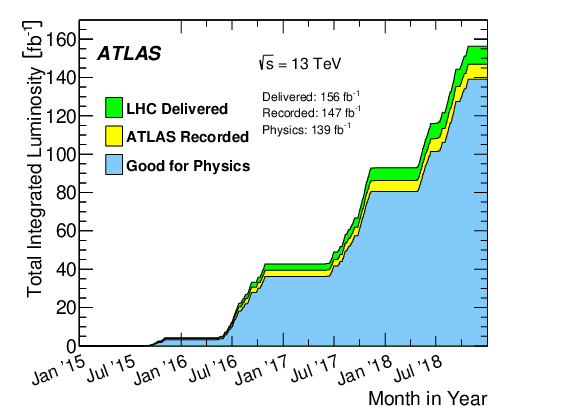
\includegraphics[scale=0.6]{figs/ch3/int_lumi.png}
  \caption{ Cumulative integrated luminosity delivered and recorded by the ATLAS detector during Run 2 of the 
  LHC between the years 2015 to 2018 with a CME of $\sqrt{\textrm{s}}$ = $\textrm{13 \ TeV}$}
\label{fig:3.2}
\end{figure}

Dense proton bunches collide in the \gls{lhc} beam line interaction points, meaning there are multiple \gls{pp} interactions at one time.
Not all interactions are considered and therefore are not saved. Typically, the most energetic collision per bunch crossing, called the hard-scatter,
is analyzed. The symbol denoting the average number of \gls{pp} collisions per bunch crossing is $\upmu$ and is termed pile-up.
The average pile-up for Run 2 is calculated to be $\langle \upmu \rangle$ = $\textrm{33.7}$. The average pile-up over each data taken year of Run 2, along with 
the total average, can be seen in Figure \ref{fig:3.3} \cite{lumi}.

\begin{figure}[h]
  \centering
  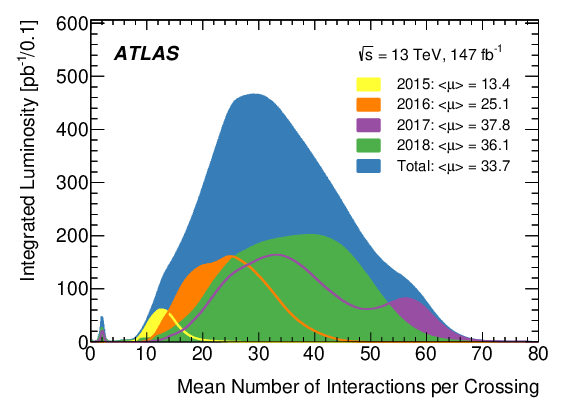
\includegraphics[scale=0.6]{figs/ch3/lumi_weight.png}
  \caption{ The $\upmu$ distribution measured by the ATLAS detector during Run 2 \cite{lumi}}
\label{fig:3.3}
\end{figure}

\section{The ATLAS Detector}

The \gls{atlas} detector is a general purpose detector located 100 meter below \gls{cern} at interaction point 1 on the \gls{lhc} ring.
The purpose of this detector is to probe the \gls{sm} using \gls{pp} collisions and \textit{Nucleus-Nucleus} collisions. Many types of physics 
analyses have been conducted using the \gls{atlas} detector, such as testing predictions for \gls{bsm} within the \gls{sm} as well as precision measurements for 
its physical parameters such as particle mass and lifetimes. The high energies provided by the \gls{lhc} allows physicists to probe very heavy particles such as the 
top quark and the Higgs boson. \gls{atlas} is the largest detector located at CERN. The detector extends 25 meters in height,
44 meters in length and weighs 7000 tons. Figure \ref{fig:3.4} shows an overview of the detector.
\par

\begin{figure}[h]
  \centering
  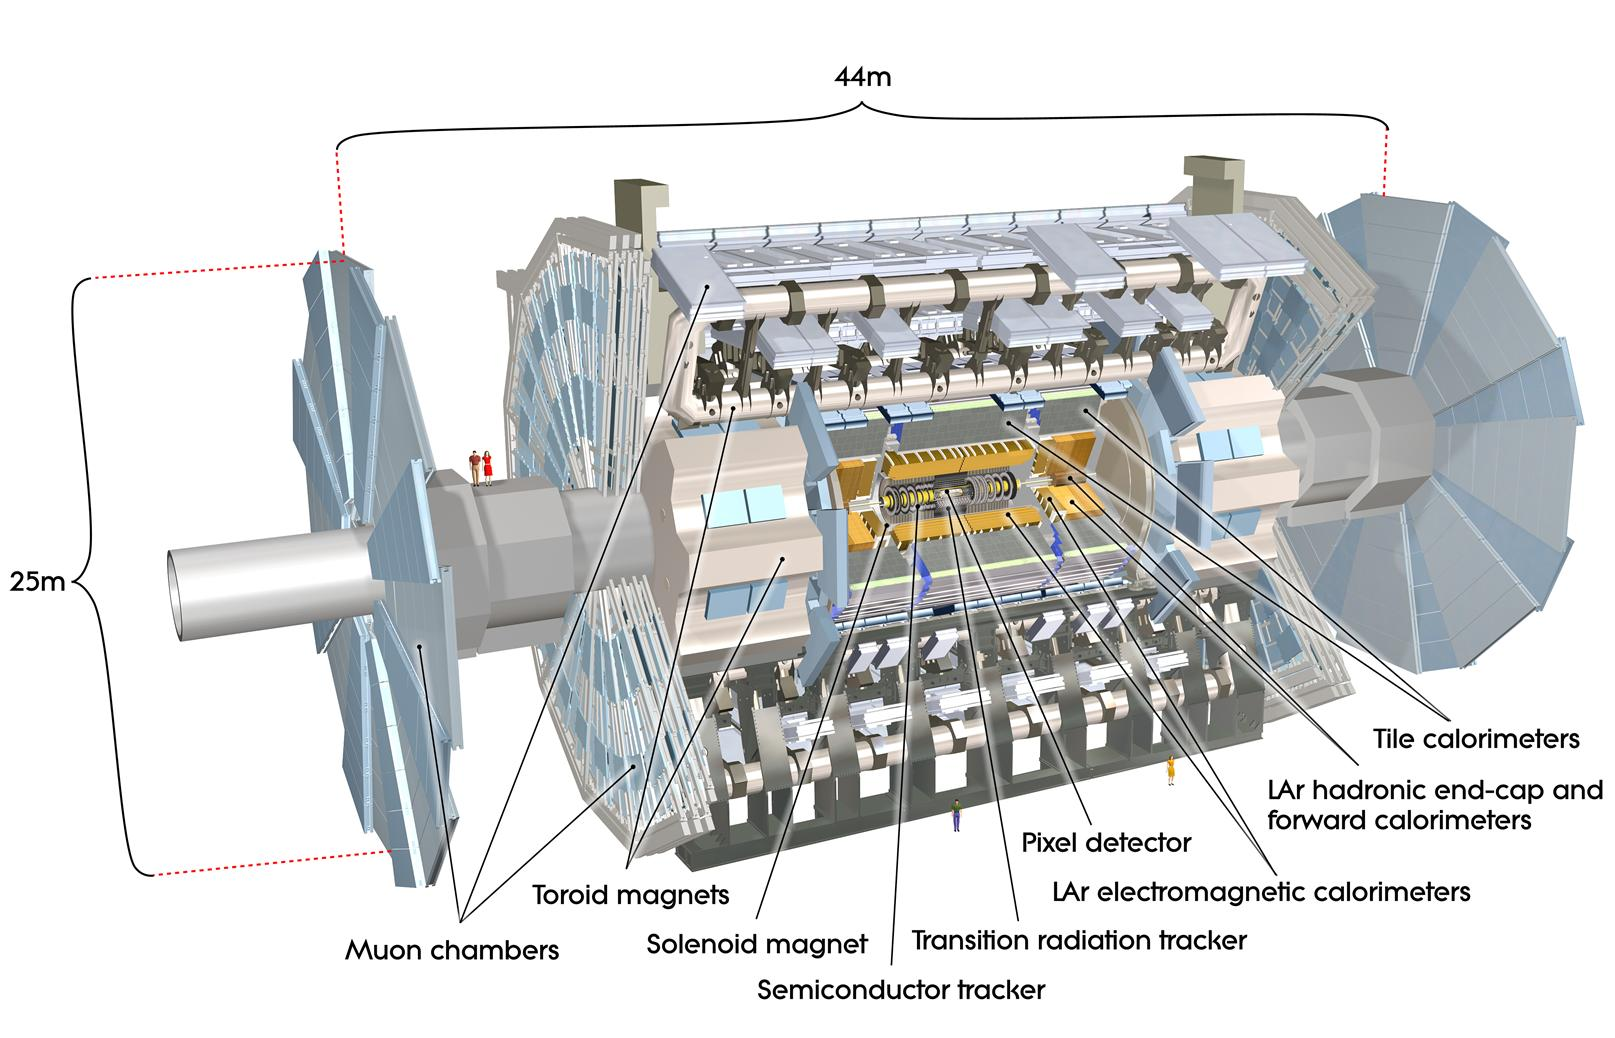
\includegraphics[scale=0.6]{figs/ch3/atlas_run2.png}
  \caption{ The ATLAS detector and its subsystems as of Run 2 \cite{atlas}}
\label{fig:3.4}
\end{figure}

The orange center of Figure \ref{fig:3.4} is the first of the sub-detectors called the Inner Detector (\gls{id}). Approximately 1000 particles are released every 25 ns, therefore high granularity is essential to differentiate the tracks of these particles. The \gls{id} is comprised 
of several parts, pixel and silicon microstrip (\gls{sct}) trackers, these are used in conjunction with the Transition Radiation Tracker (\gls{trt}.).
The \gls{id}'s main goal is to obtain the trajectories and paths of the particles that travel through it. Outside of the \gls{id} is a 
2T solenoid magnet that bends the trajectories of the particles, which allows the momentum to be calculated. After the 2T magnet are the 
calorimeters which function as energy deposition detectors. There are two types of calorimeters used, an electromagnetic calorimeter (\gls{ecal})
in which electrons deposit their energy, the second is called the hadronic calorimeter (\gls{hcal}) where hadrons deposit their energy.
Outside of these two calorimeters is the muon spectrometer (\gls{ms}) which is needed for precise muon momentum measurements. All of these systems 
form a large cylindrical shape around the \gls{lhc} beam pipe. End-caps are placed on the left and right side of the barrel which consist 
of wheel-shaped detectors.

\subsection{The Coordinate System of ATLAS}
\par

A cylindrical and a right-handed Cartesian coordinate system are used in junction within the detector
with the origin placed at the collision point. The x-axis points towards the center of the \gls{lhc}, 
the y-axis points straight up and is used for the basis of the cylindrical coordinate system. The z-axis
points directly down the beam-pipe. Two angles are used to define positions in the detector, the azimuthal angle 
$\upphi$ and pseudorapidity defined as η. Pseudorapidity is defined in Eq. \ref{eq:3.4}:
%
\begin{equation}\label{eq:3.4}
  \textrm{η} = -\textrm{ln}(\textrm{tan}(\frac{\textrm{{θ}}}{\textrm{2}}))
\tag{3.4}
\end{equation}
%
Where θ is the longitudinal angle measured between the z-axis and the trajectory of the particle. Pseudorapidity 
is an approximation of the variable rapidity and is commonly used due to its ease of calculation from the Cartesian
coordinate system and is equivalent to rapidity for massless particles. Rapidity, \textit{y}, is defined as:
%
\begin{equation}\label{eq:3.5}
  \textit{y} = \frac{\textrm{1}}{\textrm{2}}\textrm{ln}(\frac{\textrm{E}+\textrm{\textit{p}}_{\textrm{z}}}{\textrm{E}-\textrm{\textit{p}}_{\textrm{z}}})
\tag{3.5}
\end{equation}
%
Rapidity,  $∆$\textit{y}, is invariant under Lorentz boosts. A benefit of using these variables is that 
η and $\upphi$ provide a Lorentz invariant coordinate system with a distance measurement $∆$\textit{R}, 
defined as: 
%
\begin{equation}\label{eq:3.6}
  ∆\textrm{\textit{R}} = \sqrt{(∆\textrm{η})^{2}+(∆ \upphi)^{2}} 
\tag{3.6}
\end{equation}
%
Due to the physical design of \gls{atlas}, it is impossible to cover the entire η range where highly boosted particles 
are able to leave through the beam-pipe, traveling very close to the z-axis. Table \ref{table:pseudorapidity} shows the total pseudorapidity, η, range 
of all the sub-detectors. 
%
\begin{table}[h]
  \centering 
  \begin{tabular}{ |c |c |}
      \hline
      sub-detector& η coverage\\
      \hline\hline
      Inner Detector  & $\pm$ 2.5 \\
      \hline
      Electromagnetic Calorimeter & $\pm$ 3.2 \\
      \hline
      Hadronic Calorimeter & \\
      Barrel and end-cap & $\pm$ 3.2\\
      Forward Calorimeter & 3.1 < |η| < 4.9\\
      \hline
      Muon Spectrometer & $\pm$ 2.7\\
      \hline
\end{tabular}
\caption{Pseudorapidity of ATLAS sub-detectors \cite{atlas}.}
\label{table:pseudorapidity}
\end{table}

Protons from the collision point only have momentum in the \textit{z}-direction. Therefore the sum 
of the momentum in the transverse plane $\overrightarrow{\textit{P}}_{\textrm{T}} = (\textit{P}_{\textrm{x}}, \ \textit{P}_\textrm{y})^{\textrm{t}}$ 
of particles from the collision point must yield zero. Some particles, such as neutrinos or \gls{bsm} particles,
can escape the detector without depositing energy. The transverse momentum sum of all escaping 
particles can be determined from knowing that the total transverse momentum sum of all escaping particles 
must be zero. If a particle leaves without depositing energy, then the sum of the total transverse 
momentum will be negative and can be shown in the form $\overrightarrow{\textit{P}}_{\textrm{T}}^{\textrm{miss}} = - \sum_{\textrm{detected}}^{\textrm{i}}\overrightarrow{\textit{P}}_{\textrm{T}}^{\textrm{i}}$.
The absolute value of $\overrightarrow{\textit{P}}_{\textrm{T}}^{\textrm{miss}}$ is denoted as $\textrm{\textit{E}}_{\textrm{T}^{\textrm{miss}}}=|\overrightarrow{\textit{P}}_{\textrm{T}}^{\textrm{miss}}|$.
This value is referred to as missing transverse energy (\gls{met}).

\subsection{The Inner Detector}
\par
The \gls{id} consists of three independent sub-detectors that are contained within a cylindrical sleeve with 
measurements of $\pm$3512 mm and a radius of 1150 mm within a solenoid magnet of 2T. The \gls{id} has a pseudorapidity 
range of |η| $\le$ 2.5 and a $\textrm{\textit{p}}_{\textrm{T}}$ threshold of 0.5 GeV \cite{atlas}. 
The \gls{pp} collision points are contained within the \gls{id}. The collision point that contains the highest $\textrm{\textit{p}}_{\textrm{T}}$ is considered the primary vertex. As the decay products travel 
from the primary vertex, after some time, decay themselves, creating a secondary vertex point.
The \gls{id} was uniquely designed to provide robust pattern recognition and momentum resolution
for both primary and secondary vertex measurements for charged particle's tracks. The three sub-detectors provide 
complimentary data acquisition. A decay product is first met by the pixel detector, containing discrete space-points from 
silicon pixel layers. It is then met with stereo pairs of silicon micorstrip (\gls{sct}) layers. Just beyond this is the \gls{trt},
containing many layers of gaseous straw tubes interwoven with transition radiation material. Figure \ref{fig:3.5} shows a layout of the 
\gls{id}, mapping its pseudorapidity coverage and the locations of each sub-detector.

\begin{figure}[h]
  \centering
  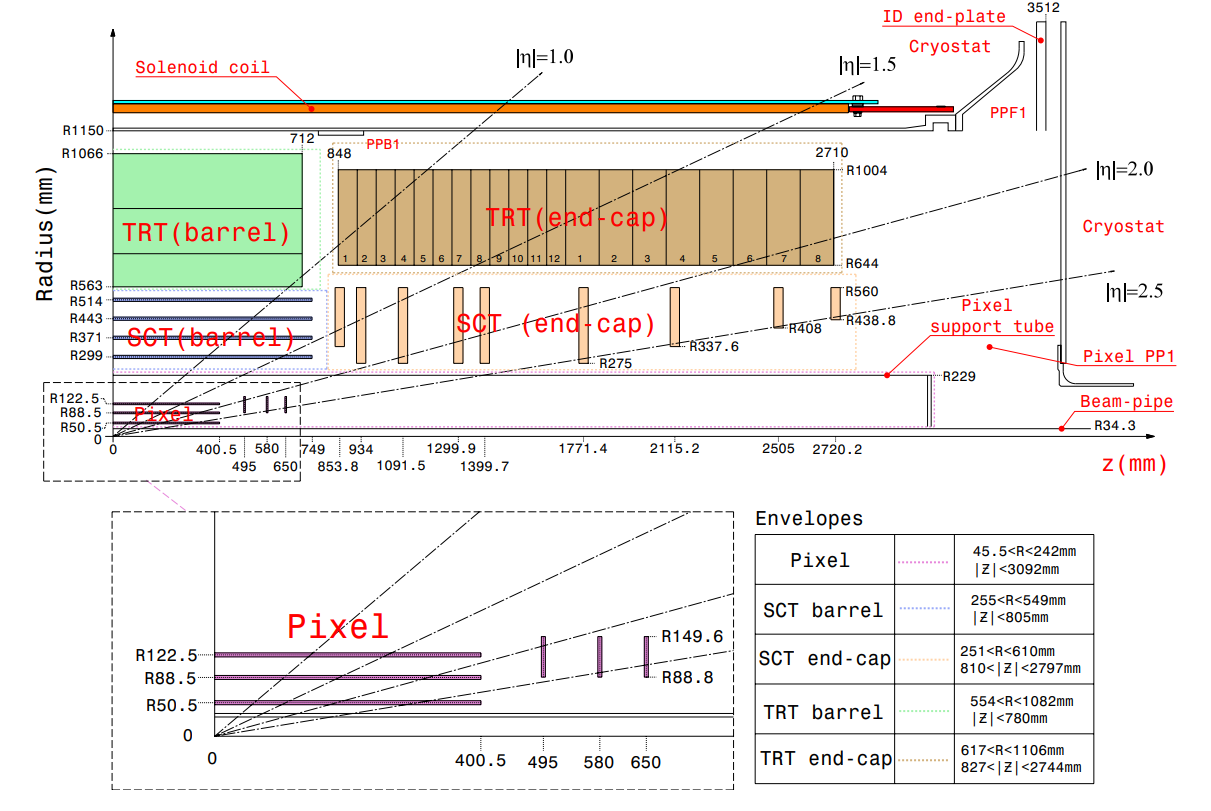
\includegraphics[scale=0.5]{figs/ch3/ID_layout.png}
  \caption{ A quarter-section of the ATLAS ID showing its major elements with their active dimensions. \cite{atlas}}
\label{fig:3.5}
\end{figure}

The \gls{pp} collisions impose a high-radiation environment which require stringent requirements for material composition 
and sensors of the \gls{id} sub-detectors. With the designed life-time of 10 years of operation during Run 2 at the \gls{lhc},
the pixel inner vertexing layer must be replaced every three years. In order to subvert radiation damage over time, the silicon 
sensors are kept at low temperatures, about -5°C to -10°C resulting in coolant temperatures of ~-25°C \cite{atlas}. The \gls{trt}
is kept at room temperature. Figure \ref{fig:3.6} shows a drawing of each sub-detector and their sensors along with a transversed track 
of a charged particle. 

\begin{figure}[h]
  \centering
  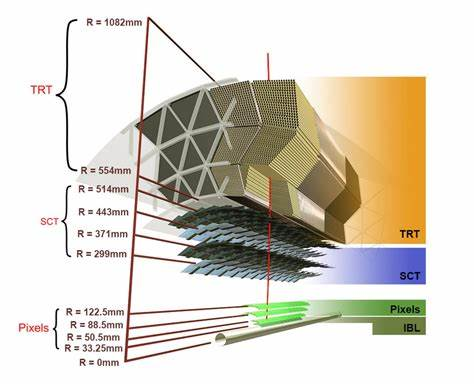
\includegraphics[scale=0.8]{figs/ch3/ID_schem.jpeg}
  \caption{ Drawing of the ID sub-detectors and their sensors. Showing the spacing of each of the sensor layers along with a transversed charged track at η=0.3. \cite{atlas}}
\label{fig:3.6}
\end{figure}

\subsubsection{The Pixel Detector}
\par

The pixel detector consists of three concentric layers of sensors in the \gls{id} barrel and three end-cap discs with sensors
parallel to the transverse plane. The barrel layers are placed at a radii of 50.5 mm, 88.5 mm, and 122.5 mm as shown in Figure \ref{fig:3.6}.
The end-cap discs are located $|\textrm{\textit{z}}|$ = 495 mm$-$650 mm and cover r = 88.8 mm$-$149.6 mm giving an eta coverage 
of $|\textrm{η}| < \textrm{2.5}$. Silicon sensors are pixelated with a pixel pitch of 50$\times$400 µ$\textrm{m}^{\textrm{2}}$ (~90\%) with the remaining being 
50 µm $\times$ 600 µ$\textrm{m}^{\textrm{2}}$. Equaling 47232 pixels per sensor. The short side of the pixel sensors are orientated along $\textrm{\textit{r}}-\upphi$ in both the barrels and the end-caps.
The pixel orientation are 10 µm along the $\textrm{\textit{r}}-\upphi$ and 115 µm in the $\textrm{\textit{z}} \ (\textrm{r})$ in the barrel (end-caps).

\subsubsection{The SCT Detector}
\par
As shown in Figure \ref{fig:3.6}, the \gls{sct} uses silicon strips distributed along four layers in the \gls{id} barrel
and nine discs in each end-cap \cite{atlas}. These layers cover ranges from \textit{r} = 299 mm to \textit{r} = 514
and cover $\textrm{\textit{z}} <$ 749 mm. The end-cap discs are placed at $|\textrm{\textit{z}}|$= 853.8 mm and 
$|\textrm{\textit{z}}|$= 2720.2 mm allowing up to |η| $\le$ 2.5 as seen in Figure \ref{fig:3.7}. The strip modules are rectangularly shaped with 
12 cm strips aligned in the \textit{z}-direction. Trapezoidal strips are implemented in the barrel end-caps. The \gls{sct} strip pitch 
is 80 µm. Three-dimensional coordinates are found by setting two strips back-to-back with an offset of 40 mrad. The intrinsic position 
of the \gls{sct} is 17 µm in the $\textrm{\textit{r}}-\upphi$ and 580 µm in $\textrm{\textit{z}} \ (\textrm{r})$ in the barrel (end-caps)

\begin{figure}[h]
  \centering
  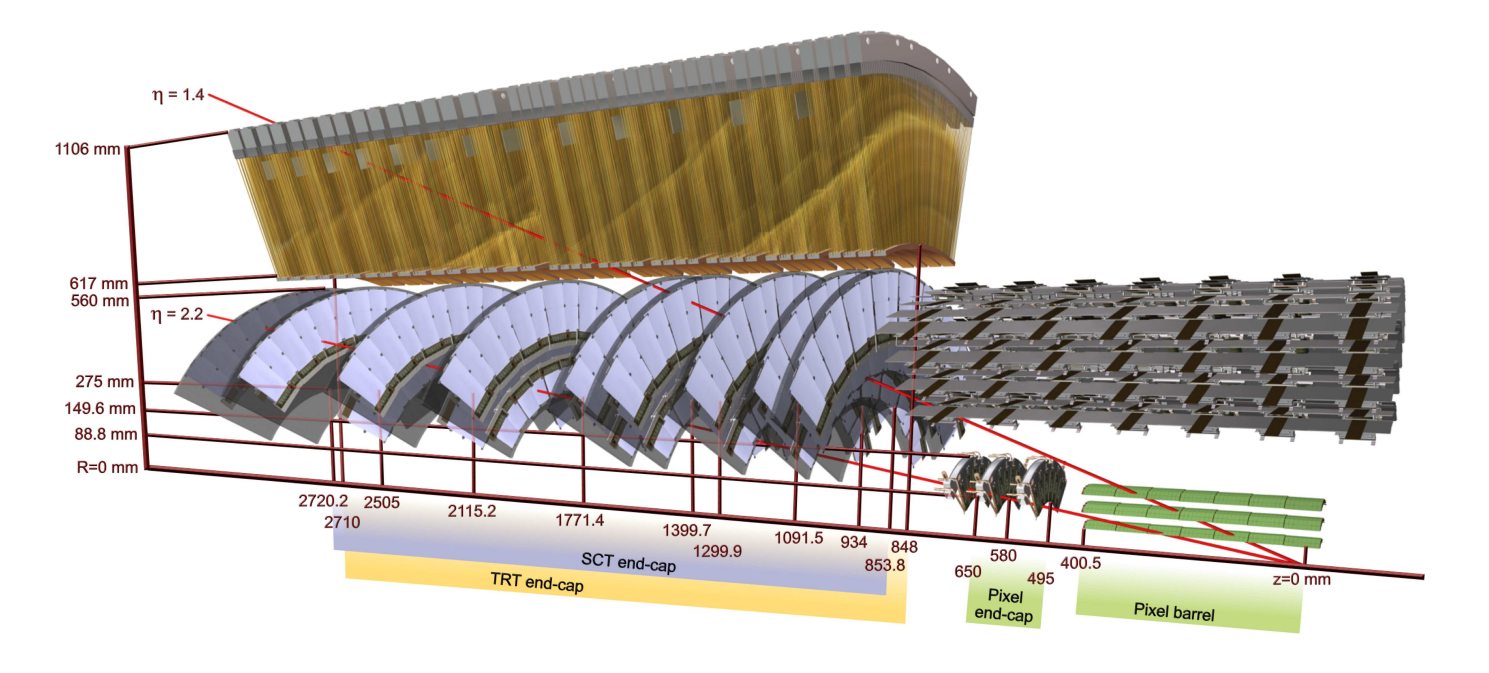
\includegraphics[scale=0.4]{figs/ch3/ID-end-caps.png}
  \caption{  Drawing of the ID sensors of all three sub-detectors and their structural elements focusing on its end-caps transversed by two charged tracks. \cite{atlas}}
\label{fig:3.7}
\end{figure}

\subsubsection{The TRT Detector}

The \gls{trt} is composed of 4 mm diameter polyimide drift straws containing a gas mixture of 70\% Xe, 27\% $\textrm{CO}_{\textrm{2}}$ and 
3\% $\textrm{O}_{\textrm{2}}$ set to 5$-$10 mbar over-pressure. The straws are made of two 35 µm thick multi-layer films bonded back-to-back.
The bare 25 µm thick polyimide film is coated on one side with a 0.2 µm Al layer which is protected by a 5-6 µm thick graphite-polyimide layer \cite{atlas}.
The straws are stabilized using carbon fibers and cut to length of 144 cm for the barrel and 37 cm for the end-caps. For the these drift tubes,
31 µm diameter tungsten anode wires plated with 0.5$-$0.7 µm gold are used and are supported by the straw ends and the end plug. These 
are connected to the electronics and kept at ground potential. Cathodes operate at $-$1530V to give a gain of $\textrm{2.5}\times\textrm{10}^{\textrm{4}}$.
The gas within the straws are ionized as a charged particle interacts with it, releasing drift electrons. These electrons are collected at 
a time of $~$48 ns. The Xe-based gas mixture requires a re-circulating gas system with continuous monitoring of its
quality. The \gls{trt} offers a particle position resolution of 130 µm which is much less than the previous two sub-detectors. The 
\gls{trt} also aids in the identification of charge particles by exploiting transition radiation. 

\subsection{The Calorimeter System}
Surrounding the \gls{id} solenoid are both of the calorimeters that are responsible for measuring charged particles Energy.
Each calorimeter consists of a number of sampling detectors that cover a full $\uppsi$-symmetry and coverage around the beam axis.
The first calorimeter is the \gls{ecal} which detect depositions of electromagnetic particles such as electrons 
and photons. Outside of the \gls{ecal} sits the hadronic calorimeter, its responsible for measuring energy of any hadronic products 
from the collision. Both calorimeter systems use liquid argon as the medium for detecting. These calorimeters have alternate between two 
types of layers, an active layer and a sampling layer. The active layer interacts with charged particles, releasing secondary particles 
that the sampling layer then measures. A calibration is done and converts the deposited energy within the sampling layer to the parent-collision 
particle's energy. 


\subsubsection{Electromagnetic Calorimeters}

\begin{figure}[h]
  \centering
  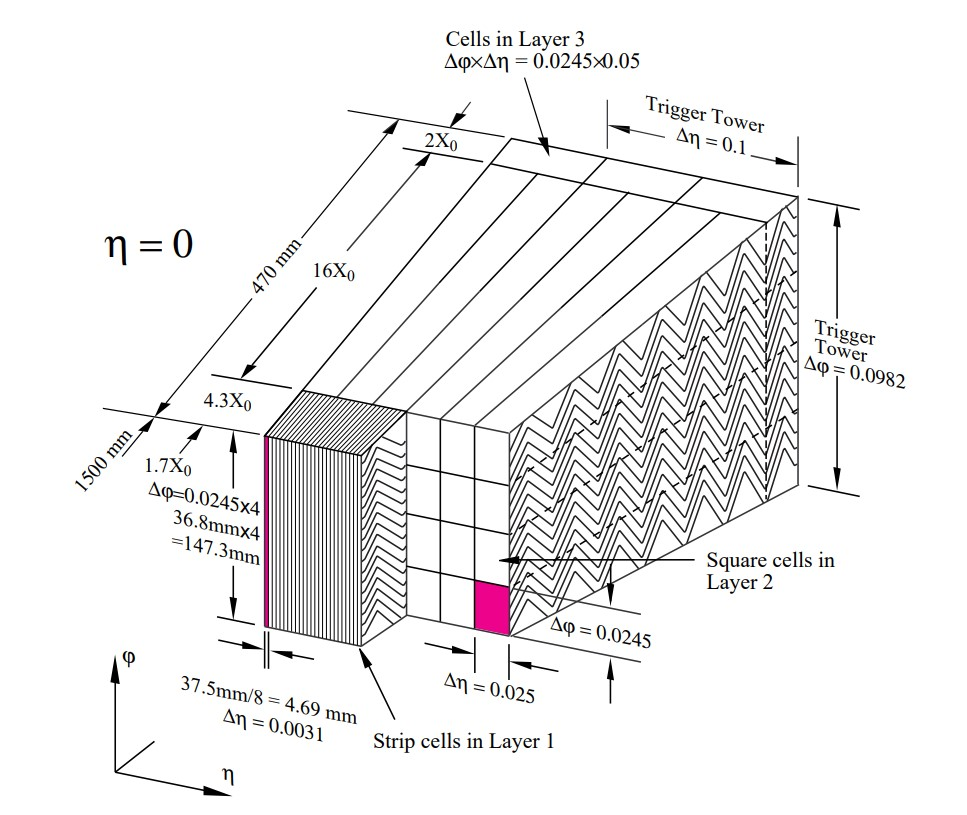
\includegraphics[scale=0.5]{figs/ch3/barrel_module.jpg}
  \caption{  Sketch of a barrel module at η=0. The folds of the electrodes and each layer's granularity is shown \cite{atlas}}
\label{fig:3.9}
\end{figure}
\par

The \gls{ecal} is just outside the solenoid of the \gls{id} and has a barrel shape with two end-caps. Inside this detector are plates
of lead laid inside two sheets of stainless steel that act as an absorber, while liquid-argon acts as the sampling material. Three 
conductive copper layers are located in the gaps between the absorbers and act as electrodes.
These electrodes and absorbers inside this calorimeter are folded in an accordion style. The folding radius varies in length to keep the liquid-argon gap constant. 
Both, the electrodes and absorbers, vary in radius with respect to the liquid-argon gap with the end-caps due to being parallel to the radial 
direction. There are two barrels that cover positive and negative η and are centered at the \textit{z} axis, called the LAr electromagnetic barrel.
One half of the barrel covers $\textrm{0} < \textrm{η} < \textrm{1.475} $ while the second half covers $\textrm{-1.475} < \textrm{η} < \textrm{0}$. The length of 
each barrel is 3.2 m, the inner and outer diameter are 2.8 m and 4 m respectively, weighing a total of 57 tons. Figure \ref{fig:3.9} 
shows a sketch of a barrel module at η = 0 showing each of the three layers and their granularity. 
\par
The end-caps of the \gls{em} calorimeters (\gls{emec}) consist of two wheels, one on each side of the barrels. Each wheel 
is 63 cm thick and weighs 27 tons. These wheels have an η coverage of $\textrm{1.375} < |\textrm{η}| < \textrm{3.2}$. A liquid-argon 
sampler is placed in the region between the wheels of the \gls{emec} and the \gls{ecal} to improve the energy measurement within 
the region which has an η coverage of $\textrm{1.5} < |\textrm{η}| < \textrm{1.8}$. Each \gls{emec} consists of two co-axial wheels located 
in between the inner and outer wheel. These are 3 mm wide and located at $|\textrm{η}|=\textrm{2.5}$.  


\begin{figure}[H]
  \centering
  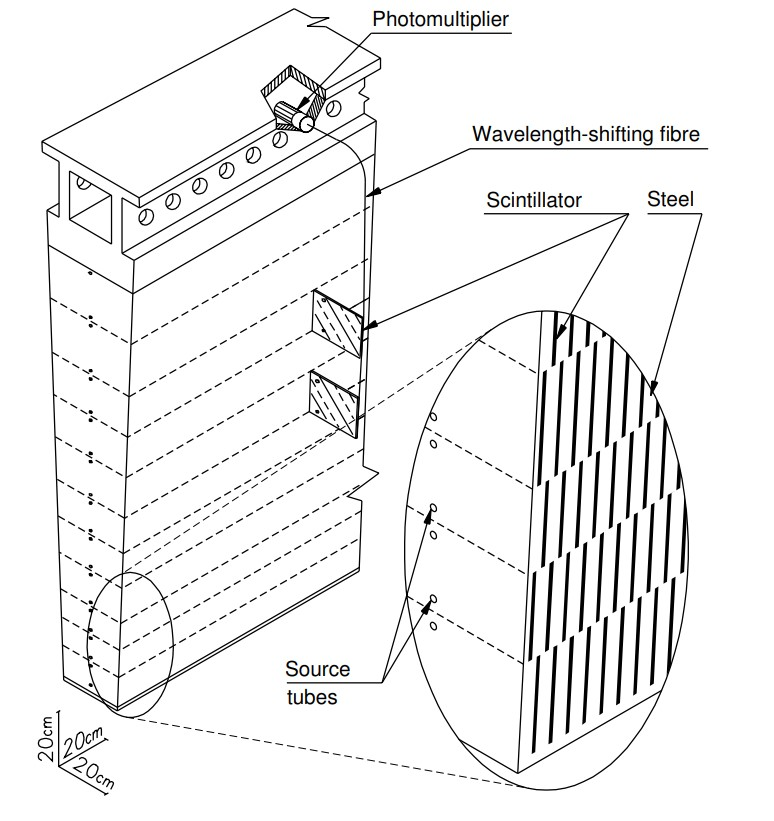
\includegraphics[scale=0.5]{figs/ch3/ecal_section.jpg}
  \caption{  Sketch of the tile calorimeter showing the alternating steel plates and scintillator material attached to PMTs. \cite{atlas}}
\label{fig:3.10}
\end{figure}

\subsubsection{Hadronic Calorimeters}

There are three sub-detectors within the \gls{hcal} system, the tile calorimeter, the liquid-argon hadronic end-cap calorimeter (\gls{hec}),
and the liquid-argon forward calorimeter (\gls{fcal}). The tile calorimeter is a sampling calorimeter that uses steel as the absorber and an 
active medium as a scintillator. It's located just outside the \gls{ecal} and covers an η region of $|\textrm{η}| < \textrm{1.7}$ and is 
divided into three parts, the center barrel extends 5.8 m in length while the two outer barrels extend 2.8 m. The orientation 
of the scintillator tiles are radial and normal to the beam line. 
Attached are wavelength-shifting fibers that extend into readout photomultiplier tubes (\gls{pmt}). A sketch of the tile calorimeter can be 
seen in Figure \ref{fig:3.10}. The output from the \gls{pmt}s are what's recorded. 
\par
The \gls{hec} schematic is shown in Figure \ref{fig:3.11}. This module is an end-cap calorimeter consisting of copper and liquid-argon sampling with 
a flat plate design, cover a range of $\textrm{1.5} < |\textrm{η}| < \textrm{3.2}$. These end-caps share the cryostats with the \
\gls{emec} and the \gls{fcal}. It consists of two wheels in each end-cap, front wheel (HEC1) and the back wheel (HEC2). Each wheel 
contains two longitudinal sections constructed of 32 identical wedge-shaped modules. The \gls{fcal} provide an η coverage of 
$\textrm{3.2} < |\textrm{η}| < \textrm{4.9}$. These modules are located at high η, approximately 4.7 m from the collision point,
exposing them to high particle fluxes. This fact resulted in much smaller liquid-argon gaps to avoid ion build-up and faster signal 
readout. Figure \ref{fig:3.12} shows an illustration of the entire \gls{hcal} section in \gls{atlas}.

\begin{figure}[H]
  \centering
  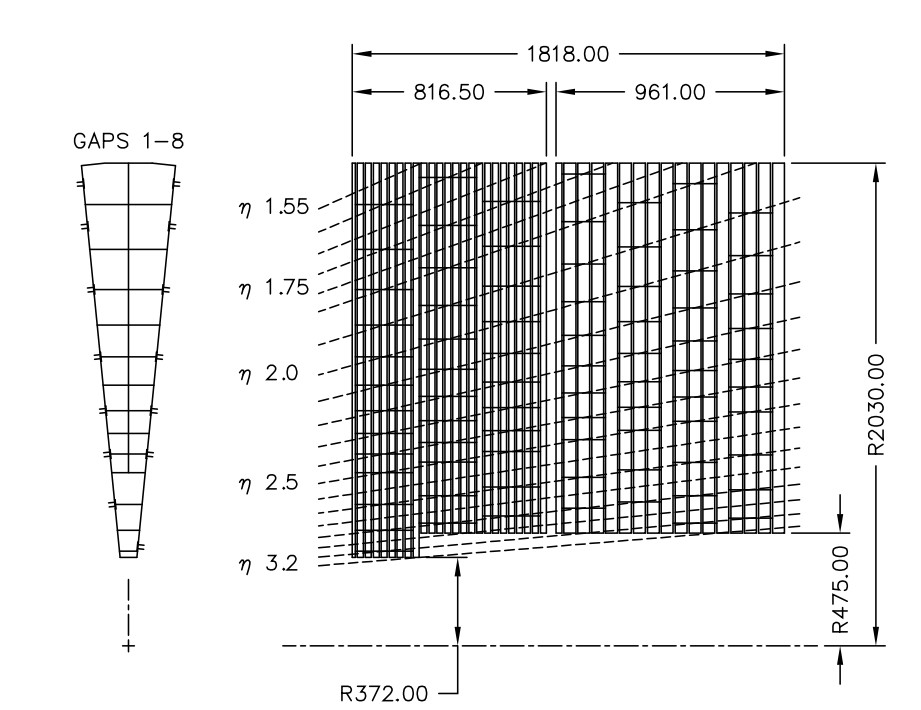
\includegraphics[scale=0.5]{figs/ch3/hcal_barrel.jpg}
  \caption{ Hadronic calorimeter end-cap. Electrode readouts indicated by dashed lines . \cite{atlas}}
\label{fig:3.11}
\end{figure}

\begin{figure}[H]
  \centering
  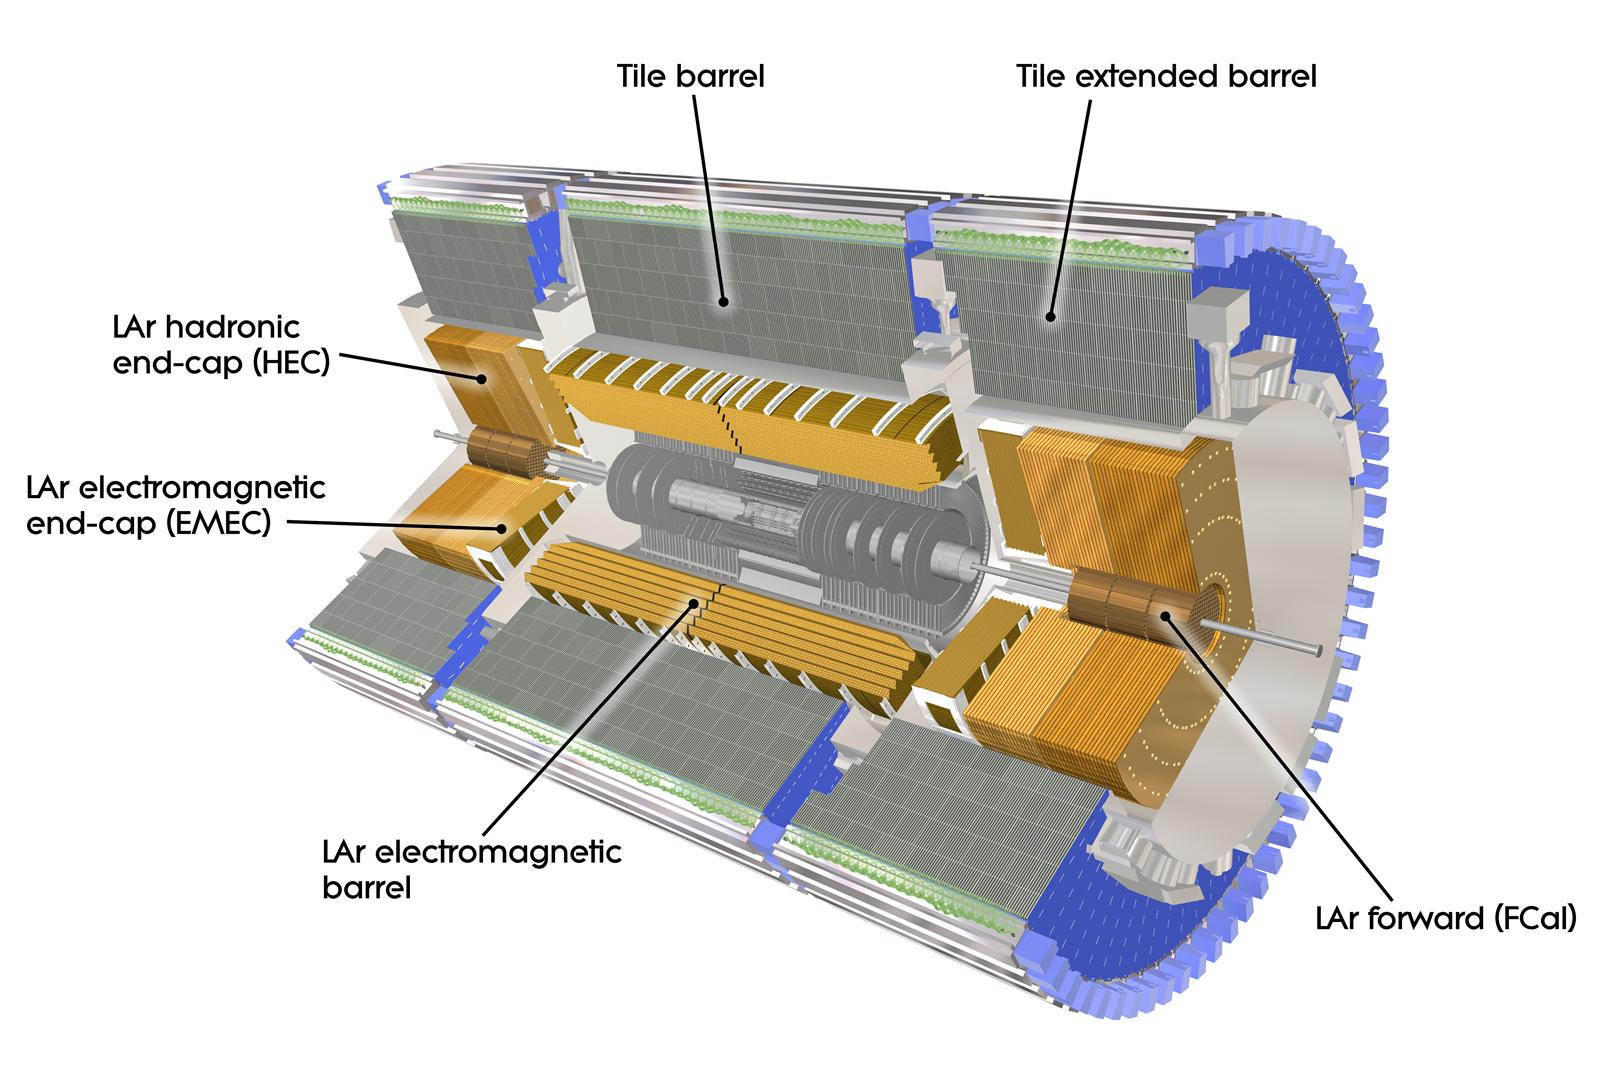
\includegraphics[scale=0.5]{figs/ch3/calorimeters.jpg}
  \caption{  Illustration of the entire HCAL system in ATLAS. \cite{atlas}}
\label{fig:3.12}
\end{figure}

\subsection{The Muon System}

The final system is the muon spectrometer which is designed to detect charged particles exiting the calorimeters 
and to measure their momentum. Muons lose minimal energy when traversing through matter and therefore are depositing minimal energy in 
the \gls{ecal}. The muon system triggers on particles with the pseudorapidity of $|\textrm{η}| < \textrm{2.4}$ and can track up to $|\textrm{η}| < \textrm{2.7}$.
The system consists of three concentric cylindrical shells of gas-filled detectors around the beam axis with radii of 5 m, 7.5 m, and 10 m.
The two end-caps of the muon chambers form large wheels, perpendicular to the \textit{z}-axis and are located 
at $|\textrm{\textit{z}}| \approx \textrm{7.4 m}$, 10.8 m, 14 m and 21.5 m from the collision point \cite{atlas}.
Figure \ref{fig:muon_sys} shows the overall arrangements in two cross-sections of the muon system. The muon trajectories are bent 
using large superconducting toroidal magnets with a generated field mostly perpendicular to the traversing muons.  
\par
The muon gas chambers are filled with 93\% Argon gas and 7\% carbon dioxide, inside the chambers are Monitored Drift Tubes (\gls{mdt}) that perform the precision momentum measurements. The layers consist of three to eight layers 
of \gls{mdt}s and can achieve an average drift resolution 80 µm per tube. In the forward region, $\textrm{2} < |\textrm{η}| < \textrm{2.7}$, Cathode-Strip Chambers (\gls{csc})
are installed within the innermost tracking layer. These are used for their high rate capability and time resolution due to the increase of particle flux. The \gls{csc} have cathodes 
perpendicular to the \gls{mdt}s and the charge induced on the cathode is measured for the signal. The resolution of each chamber is 40 µm in the bending plane (due to the toroidal magnet) and 5 mm in the transverse plane. The muon system is completed with a high precision optical alignment system and is paired with track-based alignment algorithms. 

\begin{figure}[H]
  \centering
  \subfloat[\centering Cross-section of muon system perpendicular to the beam-axis]{{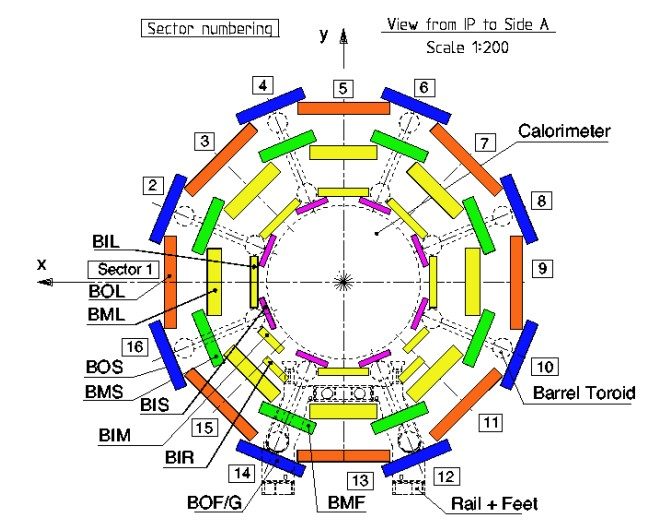
\includegraphics[scale=0.40]{figs/ch3/muon_xsec.jpg}}}%
  \qquad
  \subfloat[\centering Cross-section of muon system in a plane with the beam-axis]{{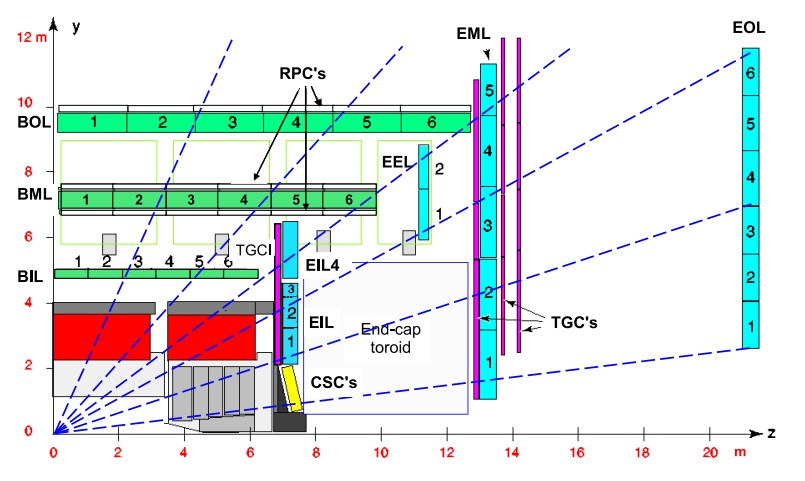
\includegraphics[scale=0.40]{figs/ch3/muon_plane.jpg}}}%
  \caption{Cross-sections of the muon system in the ATLAS detector. Figure (a) shows the three concentric cylindrical layers of 8 large and 8 small chambers. Outer diameter being 20 m. 
  Figure (b) shows a planar view of the muon system, non-bending muon tracks are shown with dashed lines \cite{atlas}}
  \label{fig:muon_sys}
\end{figure}

\subsection{Trigger and Data Acquisition}

\gls{pp} collision rate inside \gls{atlas} occurs at a very high frequency. Bunch crossings occur every 25 ns which equates to a rate of approximately 40 Mhz \cite{atlas}.
The amount of data produced in these \gls{pp} collisions exceeds the storage capabilities, additionally, most bunch crossings feature only low \gls{pp} momentum transfers and 
are therefore not interesting to analyze, let alone store. Therefore a complex selection system is implemented within \gls{atlas} called the Trigger and Data Acquisition (\gls{tdac})
system \cite{trigger}. This system is necessary to only store events that are of interest, reducing the necessity for storage facilities. 
\par
The trigger system consists of three levels of trigger systems. They are Level-1 (L1), Level-2 (L2), and event filter. The L2 and event filter triggers compose the 
High-Level Trigger (\gls{hlt}). The L1 trigger is implemented using custom-made hardware, while the \gls{hlt} is based on the latest software algorithms. The highest 
acceptance rate of the L1 trigger is 75 kHz and the decision making must reach the front-end electronics within 2.5 µs. This trigger mainly searches for signatures from 
high-$\textit{\textit{p}}_{\textrm{T}}$ muons, electrons, photons, jets, $\tau$-leptons that decay into hadrons, and \gls{met} using information collected by the calorimeters and muon 
spectrometer. Figure \ref{fig:3.14} shows a diagram for the L1 trigger. This information is passed to the L2 trigger which reduces the event rate to below 3.5 kHz. The L2 separates this information into Regions-of-Interest (RoI) 
based on coordinates, energy and types of signatures. The event filter uses offline analysis procedures to further reduce the dataset by down to approximately 200 Hz by making decisions 
on fully built events. However, the average acceptance rate of the \gls{hlt} is 1.2 kHz, corresponding to a data rate of 1.2 GB$\textrm{s}^{\textrm{-1}}$ to be written to disc \cite{trigger}. 

\begin{figure}[H]
  \centering
  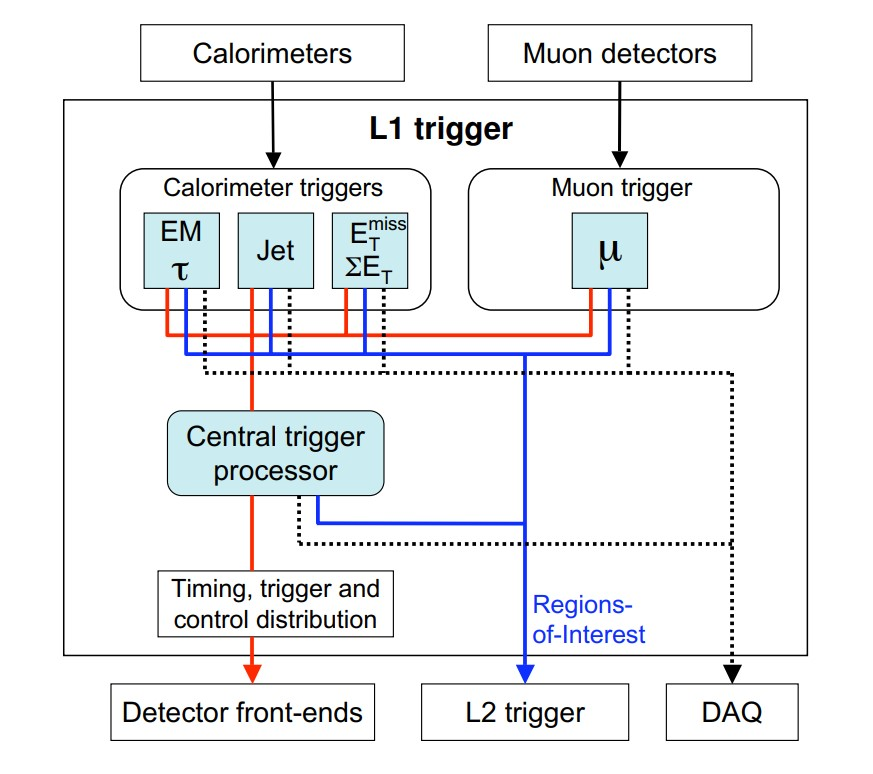
\includegraphics[scale=0.4]{figs/ch3/L1-diagram.jpg}
  \caption{ Block diagram of the L1 trigger in the ATLAS detector showing data paths to the front-end, L2 trigger and DAQs system. \cite{atlas}}
\label{fig:3.14}
\end{figure}

\section{The High-Luminosity LHC and the ATLAS Detector Upgrade}\label{sec:hllhc-itk}

There are two crucial factors in defining rare physics searching capabilities, one is the \gls{cme} and the other is integrated luminosity. The \gls{cme} dictates the 
production cross-section for each physics process, allowing for the produced particle to shift from off-shell (produced at a non-theorized mass) to on-shell (produced at 
theorized mass). Increasing the luminosity equates to increasing the total data production, therefore increasing the amount of rare events one may be looking for. The \gls{lhc} was 
initially designed to run at a \gls{cme} of 14 TeV in which it has obtained a value of 13.6 TeV during Run 3. The current luminosity obtained as been 140 f$\textrm{b}^{\textrm{-1}}$
during Run 2 and an estimated 300 f$\textrm{b}^{\textrm{-1}}$ during the course of the ongoing Run 3. 
\par
The \gls{hllhc} is aimed to fully utilize the capabilities of the \gls{lhc} with a running lifetime of 12 years (called Run 4). It is designed to increase the number of collisions per bunch 
crossing from $\langle \upmu \rangle$ = $\textrm{33.7}$ to $\langle \upmu \rangle$ = $\textrm{200}$. The expected peak luminosity achieved by the \gls{hllhc} is $\textrm{5} \times \textrm{10}^{\textrm{34}} \ \textrm{cm}^{\textrm{-2}}\textrm{s}^{\textrm{-1}}$
The expected integrated luminosity of each year is 250 f$\textrm{b}^{\textrm{-1}}$, with a total of 3000 f$\textrm{b}^{\textrm{-1}}$ after the 12 year run time \cite{hllhc-tech}.
This massive upgrade to the \gls{lhc} requires systems to be upgraded and some to be fully exchanged since these systems are vulnerable to breaking down due to high radiation 
exposure. This increase in radiation is also taken into account within the \gls{atlas} detector, realizing the current infrastructure within the detector is unable 
to withstand this amount of radiation for the running time of Run 4. This high information dense environment now imposes a few new challenges, such as maintaining high 
granularity data readout and the ability for the electronics to maintain this operative power under such high radiation doses. In order to obtain this new feat, the \gls{id} 
will be completely replaced with a new detector sub-system called the Inner Tracker (\gls{itk}) as a part of the \gls{atlas} Upgrade. Part of the work in this thesis 
focuses on preliminary studies of the latest particle identification algorithms implementing the new geometry imposed by the \gls{itk} through computer simulations.

\subsection{The Inner Tracker}

The new tracking detector is designed for a 10 year life span of operation at instantaneous luminosity of 
7.5$\times \textrm{10}^{\textrm{34}}\textrm{cm}^{\textrm{-2}}\textrm{s}^{\textrm{-1}}$, 25 ns per bunch crossing and a total 
integrated luminosity of 3000 f$\textrm{b}^{\textrm{-1}}$ over the entire lifetime \cite{itk-tech}. The current solenoid magnet being used will remain in place and 
provide a magnetic field of 2T as per the previous runs. One of the major improvements (besides being radiation hard) is that the new design will allow 
data collection of quality events of up to $|\textrm{η}| < \textrm{4.0}$. This is achieved through a complex system of silicon barrel layers and disks or rings along with 
inclined pixel modules to have better coverage between the barrel and the end-caps of the \gls{itk}. The barrel will extend $\textrm{η} \approx\pm \textrm{1}$ 
in which the current \gls{id} barrel only has a $\textrm{η} \approx\pm \textrm{0.6}$ coverage.

\subsubsection{ITk Layout}

In the central area in the \gls{itk} barrel, sensors are arranged in cylinders around the beam axis. The first five layers are pixel modules followed by two short-strip layers 
of stereo modules then followed by two even longer strip stereo modules. The forward η regions will be covered using six strip disks on either side and several pixel 
rings. 

\begin{figure}[H]
  \centering
  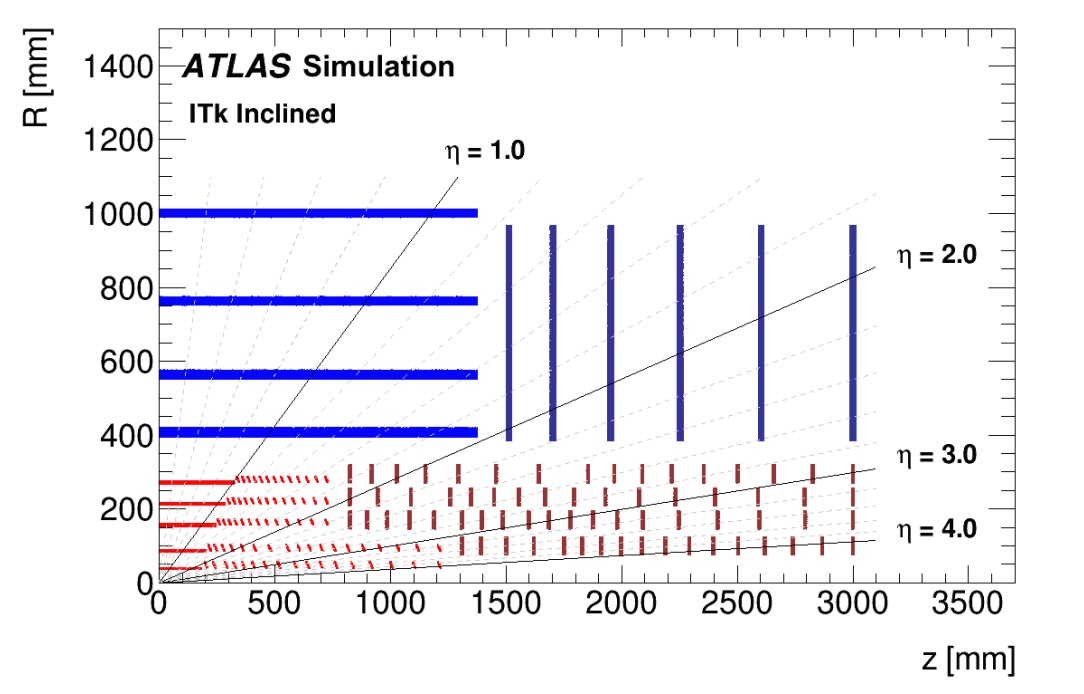
\includegraphics[scale=0.6]{figs/ch3/itk-layout.jpg}
  \caption{ The ITk layout. The pixel detectors are shown in red and the strip Detector in blue.  \cite{itk-tech}}
\label{fig:3.15}
\end{figure}

The strip detectors seen in blue in Figure \ref{fig:3.15} consists of four-layer barrel sections and one end-cap on each side containing six disks. 
This strip system covers $\textrm{η} \approx\pm \textrm{2.7}$ in the barrel region and sits $\pm$ 1400 mm along the \textit{z}-axis. 
The inner layer strips extend a length of 24.1 mm while the outer layer strips are 48.2 mm. All strips within the \gls{itk} have a pitch of 75.5 µm.
Table \ref{table:itk-strip} shows layout parameters of the strip detectors within the detector barrel. 
\par

\begin{table}[t]
  \centering 
  \begin{tabular}{ |c |c |c |c |c |c |}
      \hline
      \multicolumn{6}{|c |}{ITk Barrel Strip Detector Layout Parameters}\\
      \hline\hline
      Layer& Radius [mm]& Channels in $\upphi$& Strip Pitch [mm]& Strip Length [mm]& Tilt Angle [◦]\\
      \hline
      0 & 405 & 28$\times$1280 & 75.5 & 24.1 & 11.5 \\
      1 & 562 & 40$\times$1280 & 75.5 & 24.1 & 11.5 \\
      2 & 762 & 56$\times$1280 & 75.5 & 48.2 & 10 \\
      3 & 1000 & 72$\times$1280 & 75.5 & 48.2 & 10 \\
      \hline
\end{tabular}
\caption{Layout Parameters of the ITk Strip Detector barrel. Each strip is 2.8 m long. \cite{itk-tech}.}
\label{table:itk-strip}
\end{table}

The strips in the six end-cap wheels on each side are radially distributed, pointing towards the \textit{z}-axis. The 
strips vary in length within these end-caps to optimize total strip occupancy, starting at 19.0 mm closer to 
the beam axis, varying up to 60.1 mm in the outermost regions. The exact locations of the end-cap disks and 
strips are shown in table \ref{table:itk-strip-EC}.
\par
Aside from the strip detectors within the \gls{itk}, there are pixel detectors as shown in red in Figure \ref{fig:3.15}. The pixel detector consists of five barrel layers and 
four end-cap ring layers. The layout provides a full eta coverage of  $|\textrm{η}| = \textrm{4}$. The design of the pixel detector allows it to be operating the full lifetime of
12 years. The barrel layer of pixel sensors are placed tangentially of the constant radius of the cylindrical barrel shape. The sensors in the forward parts of the barrel 
are inclined at an angle of 56$^\circ$. Currently, each pixel size is nominally set to 50$\times$50 µ$\textrm{m}^{\textrm{2}}$ with a thickness of 100 µm for the two most inner 
barrel layers and 150 µm for the outer two for simulation. 

\subsection{B-Tagging and Vertex Reconstruction for the ITk}

Event reconstruction is crucial to the integrity of all physics conducted at the \gls{lhc}. In order to effectively reconstruct events, the energy deposition and associated 
tracks must be recorded for the specified event to be rebuilt. As stated earlier, at the \gls{hllhc} it is expected to obtain a pile-up of $\langle \upmu \rangle$ = $\textrm{200}$.
This means the mean separation of primary vertices will be approximately less than 1 mm within the space of the \gls{itk} barrel. Meaning it's not possible for all primary 
vertices of each event to be reconstructed independently. Therefore, it's crucial that all high energetic events coming from a common vertex must be identified to a 
high efficiency. Vertex reconstruction within such an environment imposed strict requirements on tracking resolution close to the particle interaction points. The goal 
is to have reconstructed vertices for $t\overbar{t}$ events to be greater than 0.95 and that the $t\overbar{t}$ decay product is associated to the correct vertex 
at a rate greater than 0.90. The b-tagging versus light-jet rejection should be optimized for each layout and at minimum should match the performance of the \gls{id}.
There is a much more in depth discussion on particle identification and event simulation in chapters~\ref{sec:track-reco} and \ref{sec:event-sim} respectively. 

\subsection{High Granularity Timing Detector}\label{sec:hgtd}

The High Granularity Timing Detector (\gls{hgtd}) is a disc shaped detector that will be placed outside the \gls{itk}. It will be added in front to the end cap and forward calorimeters at 
$|\textrm{\textit{z}}|$= 3.5m. It is composed of two forward and backwards disks with central half rings and stave concepts with a total area of 6 $\textrm{m}^{\textrm{2}}$ of silicon sensors.
The \gls{hgtd} offers a new and powerful technique to overcome the obstacle of pile-up. It takes advantage of the time spread of interactions that occur close in space but spread apart over time. 
This provides a time resolution with a precision measurement of up to 30 ps and will cover an $\textrm{2.4} < |\textrm{η}| < \textrm{4.0}$ where pile-up is rejected \cite{hgtd}.
Figure \ref{fig:3.16} shows the assembly diagram of the \gls{hgtd}

\begin{figure}[ht]
  \centering
  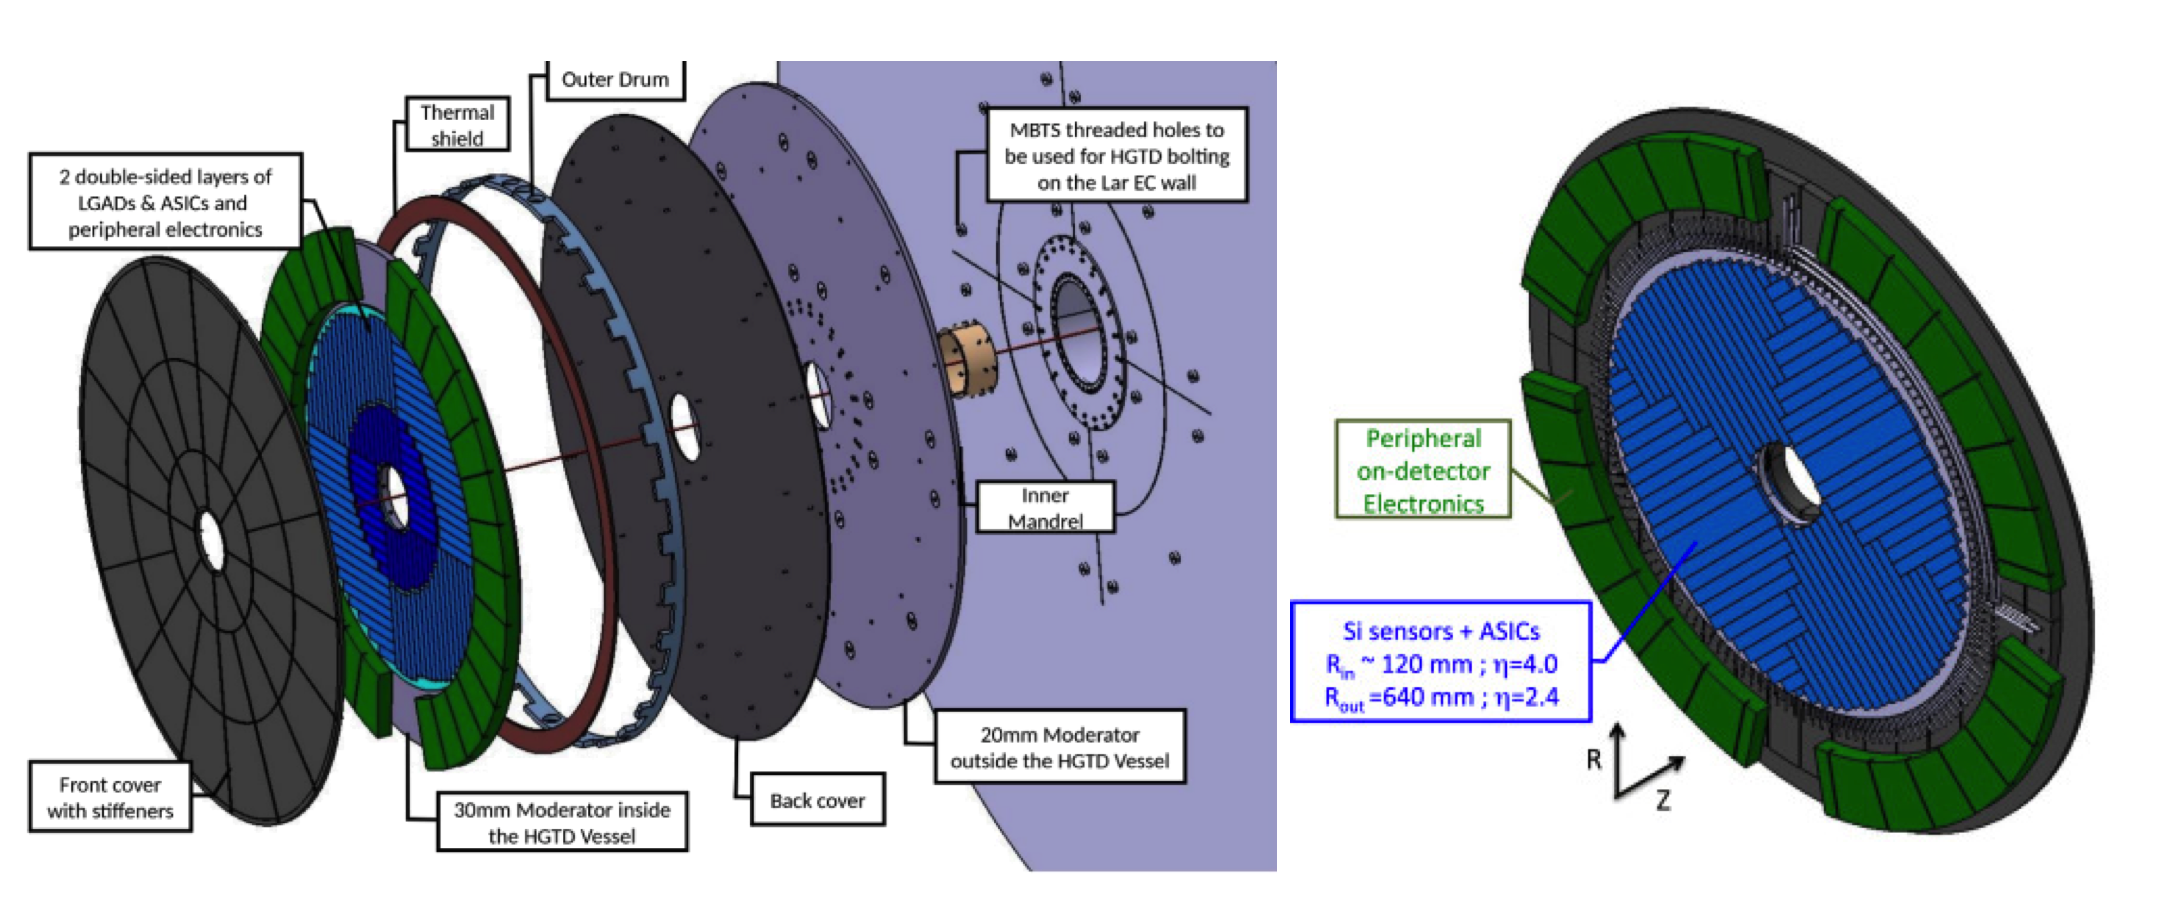
\includegraphics[scale=0.4]{figs/ch3/hgtd_assem.png}
  \caption{ The assembly of the HGTD detector\cite{hgtd}}
\label{fig:3.16}
\end{figure}

The sensors that are built within the \gls{hgtd} are referred to as Low Gain Avalanche Detectors (\gls{lgad}s). 
These sensors will have an active thickness of 50 µm and the pixel area covers 1.3 $\times$ 1.3 $\textrm{mm}^{\textrm{2}}$. The 
sensors will be integrated to an electronic circuit that is currently being developed to meet the requirements of the necessary 
timing resolution and radiation hardness \cite{hgtd}. The \gls{lgad} sensors are n-on-p silicon detectors with an internal gain. 
To obtain this gain, a highly doped, p-layer is added just below the p-n junction. This doped region creates a very high electric 
field and will induce an avalanche of the electrons and thus creating additional electron-hole pairs. Figure~\ref{fig:3.17} shows an illustration 
of the \gls{hgtd}. The blue represents the active \gls{lgad} region and the green is an inactive off-detector region.

\begin{figure}[H]
  \centering
  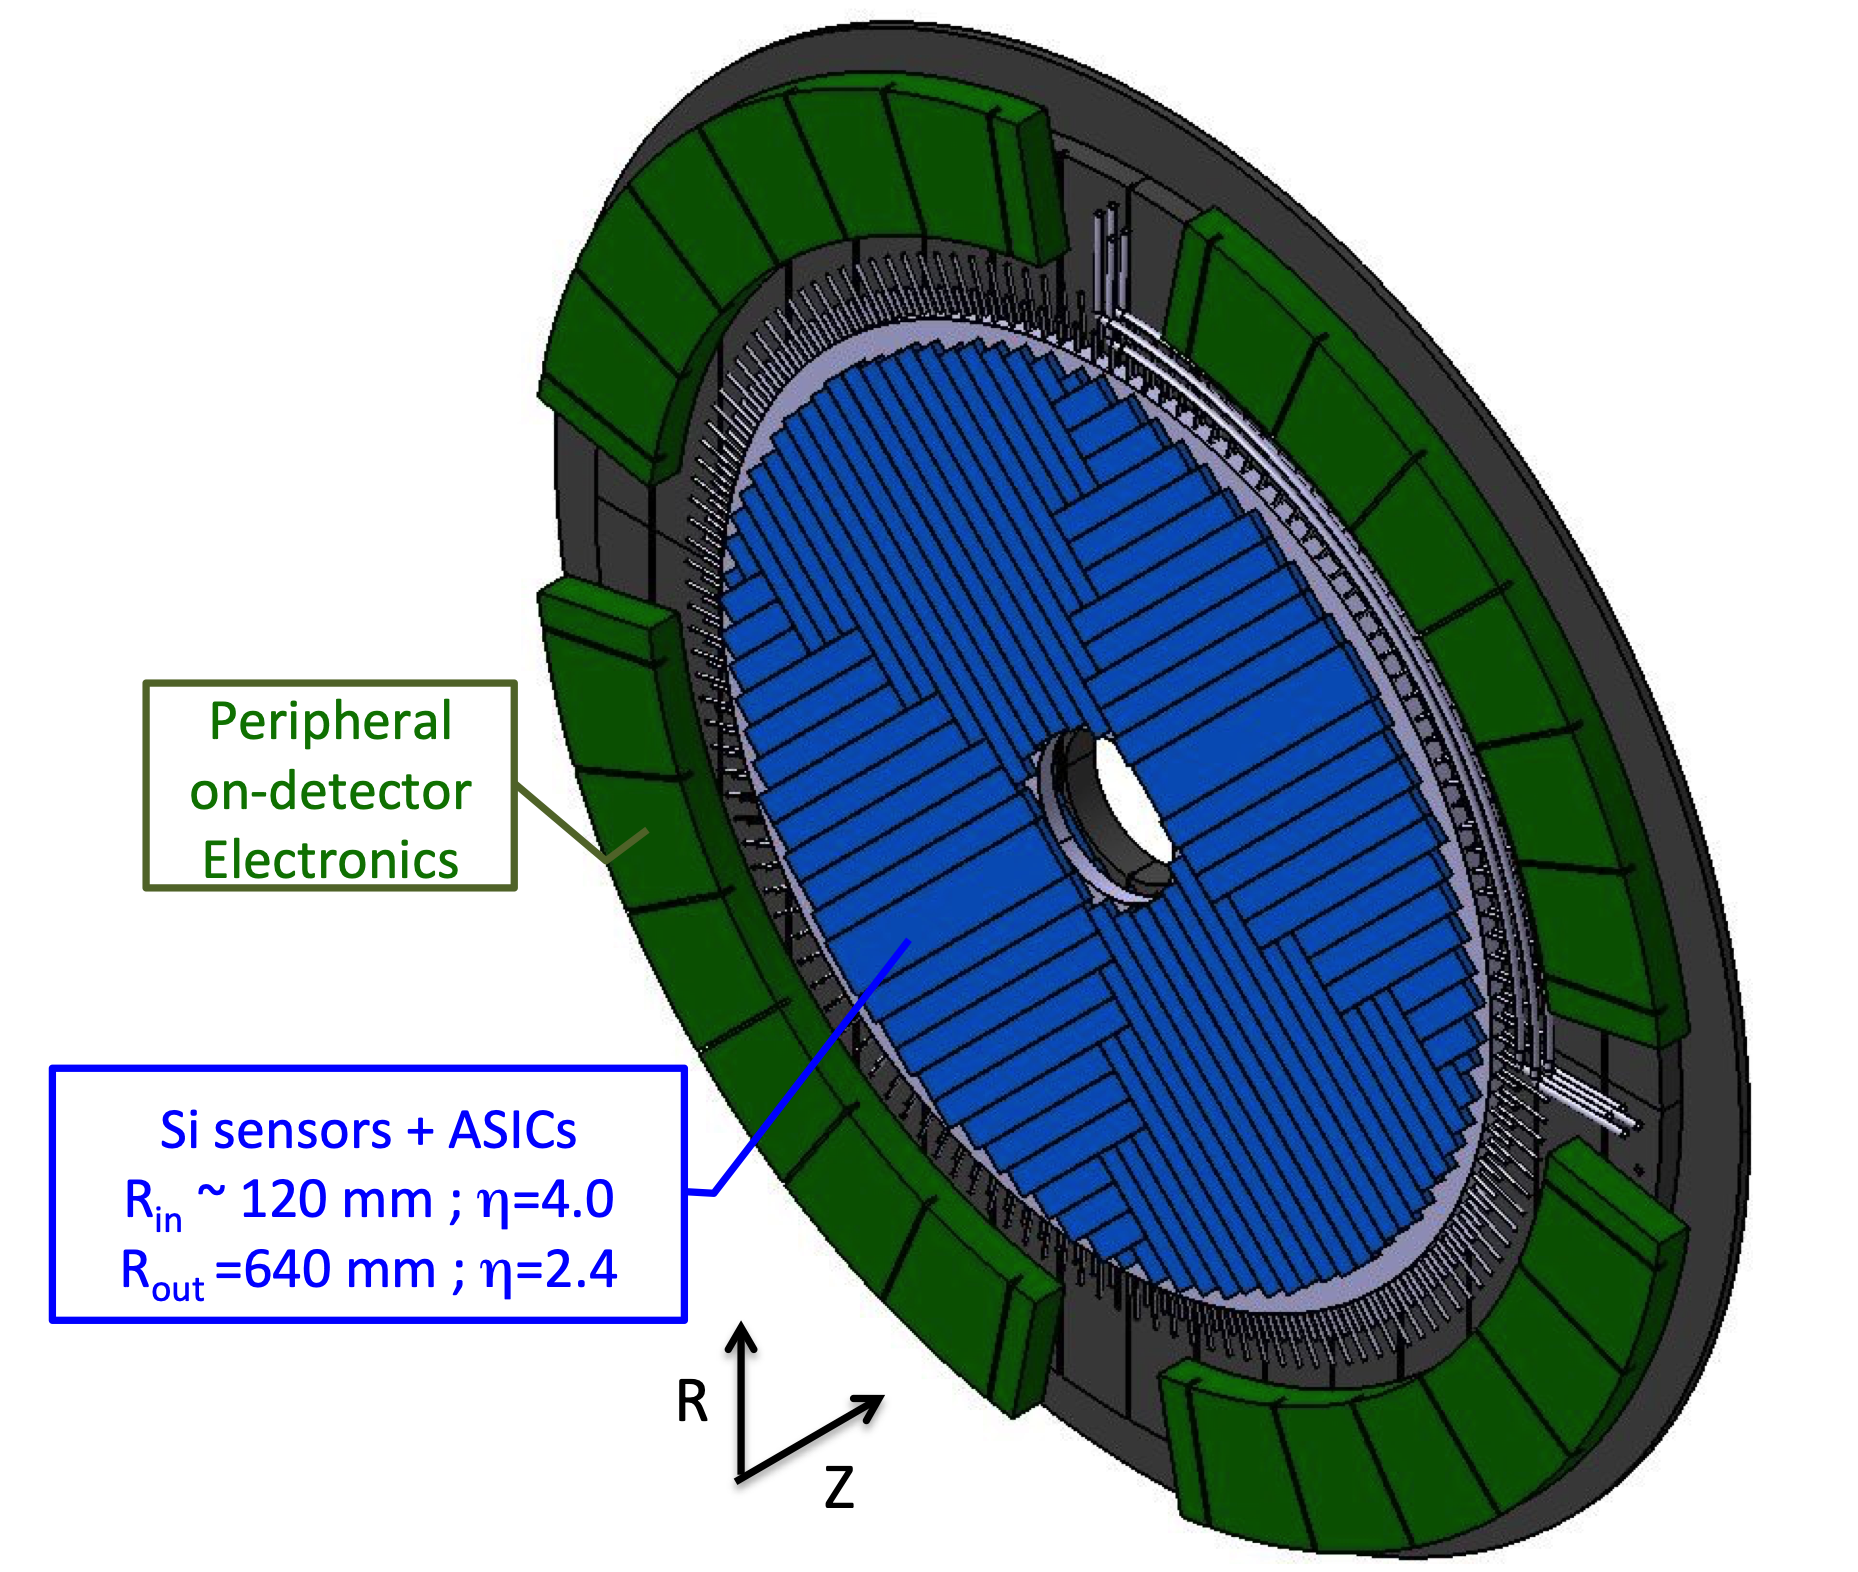
\includegraphics[scale=0.4]{figs/ch3/hgtd_disc.png}
  \caption{ An illustration of the HGTD showing the LGAD sensors (blue) and an inactive region off-detector (green) \cite{hgtd}}
\label{fig:3.17}
\end{figure}

\begin{table}[H]
  \centering 
  \begin{tabular}{ |c |c |c |c |}
      \hline
      \multicolumn{4}{|c |}{ITk Barrel Strip Detector Layout Parameters}\\
      \hline\hline
      Ring/Row & Inner Radius [mm]& Strip Pitch [mm]& Strip Length [mm]\\
      \hline
      Ring 0 Row 0 & 384.5 & 75.0 & 19 \\
      Ring 0 Row 1 & 403.5 & 79.2 & 24 \\
      Ring 0 Row 2 & 427.5 & 74.9 & 29 \\
      Ring 0 Row 3 & 456.4 & 80.2 & 32 \\
      \hline
      Ring 1 Row 0 & 489.8 & 69.9 & 18.1 \\
      Ring 1 Row 1 & 507.9 & 72.9 & 27.1 \\
      Ring 1 Row 2 & 535   & 75.6 & 24.1 \\
      Ring 1 Row 3 & 559.1 & 78.6 & 15.1 \\
      \hline
      Ring 2 Row 0 & 575.6 & 75.7 & 30.8 \\
      Ring 2 Row 1 & 606.4 & 79.8 & 30.8 \\
      \hline
      Ring 3 Row 0 & 638.6 & 71.1 & 32.2 \\
      Ring 3 Row 1 & 670.8 & 74.3 & 26.2 \\
      Ring 3 Row 2 & 697.1 & 77.5 & 26.2 \\
      Ring 3 Row 3 & 723.3 & 80.7 & 32.2 \\
      \hline
      Ring 4 Row 0 & 756.9 & 75.0 & 54.6 \\
      Ring 4 Row 1 & 811.5 & 80.3 & 54.6 \\
      \hline
      Ring 5 Row 0 & 867.5 & 76.2 & 40.2 \\
      Ring 5 Row 1 & 907.6 & 80.5 & 60.2 \\
      \hline
\end{tabular}
\caption{Main layout parameters for the strip detector end-caps. \cite{itk-tech}.}
\label{table:itk-strip-EC}
\end{table}
\begingroup
\clearpage% Manually insert \clearpage
\let\clearpage\relax% Remove \clearpage functionality
\vspace*{-16pt}% Insert needed vertical retraction
\chapter[OBJECT RECONSTRUCTION AND EVENT SIMULATION IN ATLAS]{OBJECT RECONSTRUCTION AND EVENT SIMULATION IN ATLAS}
\label{ch4}
\endgroup

The previous chapter went into detail on how the \gls{atlas} detector works through its various sub-detectors and and systems. Collisions occur at the beam axis, creating a shower 
of particles into the detector, depositing energy on an object's corresponding detector and having its tracks mapped by several systems within the \gls{id}. These recorded signals 
from \textit{triggered} events are used to reconstruct the event using complex algorithms. 
\par
Figure 18 shows a slice of the \gls{atlas} sub-detectors with several different objects from a single event depositing energy in corresponding sensors. The trajectories 
of charged particles (tracks) are reconstructed using the \gls{id} \cite{atlas}. Muons are reconstructed using associated tracks measured within the muon spectrometer and 
tracks left within the \gls{id} \cite{muon-reco}. Electrons are reconstructed using tracks detected within the \gls{id} along with energy deposits within the \gls{ecal} \cite{e-y_performance}.
Photons will also deposit their energy within the \gls{ecal}, but do not leave any tracks, thus being able to separate both electromagnetic objects. 
\par
From these collision events are objects known as jets, i.e., hadron cones due to hadronization of quarks and gluons as seen in Figure \ref{fig:4.1} as the red deposits in the blue \gls{hcal}.
Due to hadronization, multiple tracks are associated with jets which is why jets are reconstructed and not individual hadrons. Jets can be caused by several different hadrons 
and so we separate these types into, what we call, flavors. Jets caused by \textit{b}-hadrons are called \textit{b}-jets, and likewise, \textit{c}-hadrons cause \textit{c}-jets. 
The lighter quarks (up, down and strange as discussed in Section \ref{sect:standard_model}) are difficult to differentiate due to their similar size in mass. We group these hadrons 
into a single category of jets called \textit{light}-jets. As jets propagate outward they create a cone like shape within the \gls{hcal}, covering an angular 
area. Jets that cover a large angular area are considered large-radius jets \cite{large-r-jets} which contain interesting physics and are a focused object for the preliminary 
analysis in the last chapter of this thesis. 

\begin{figure}[h]
    \centering
    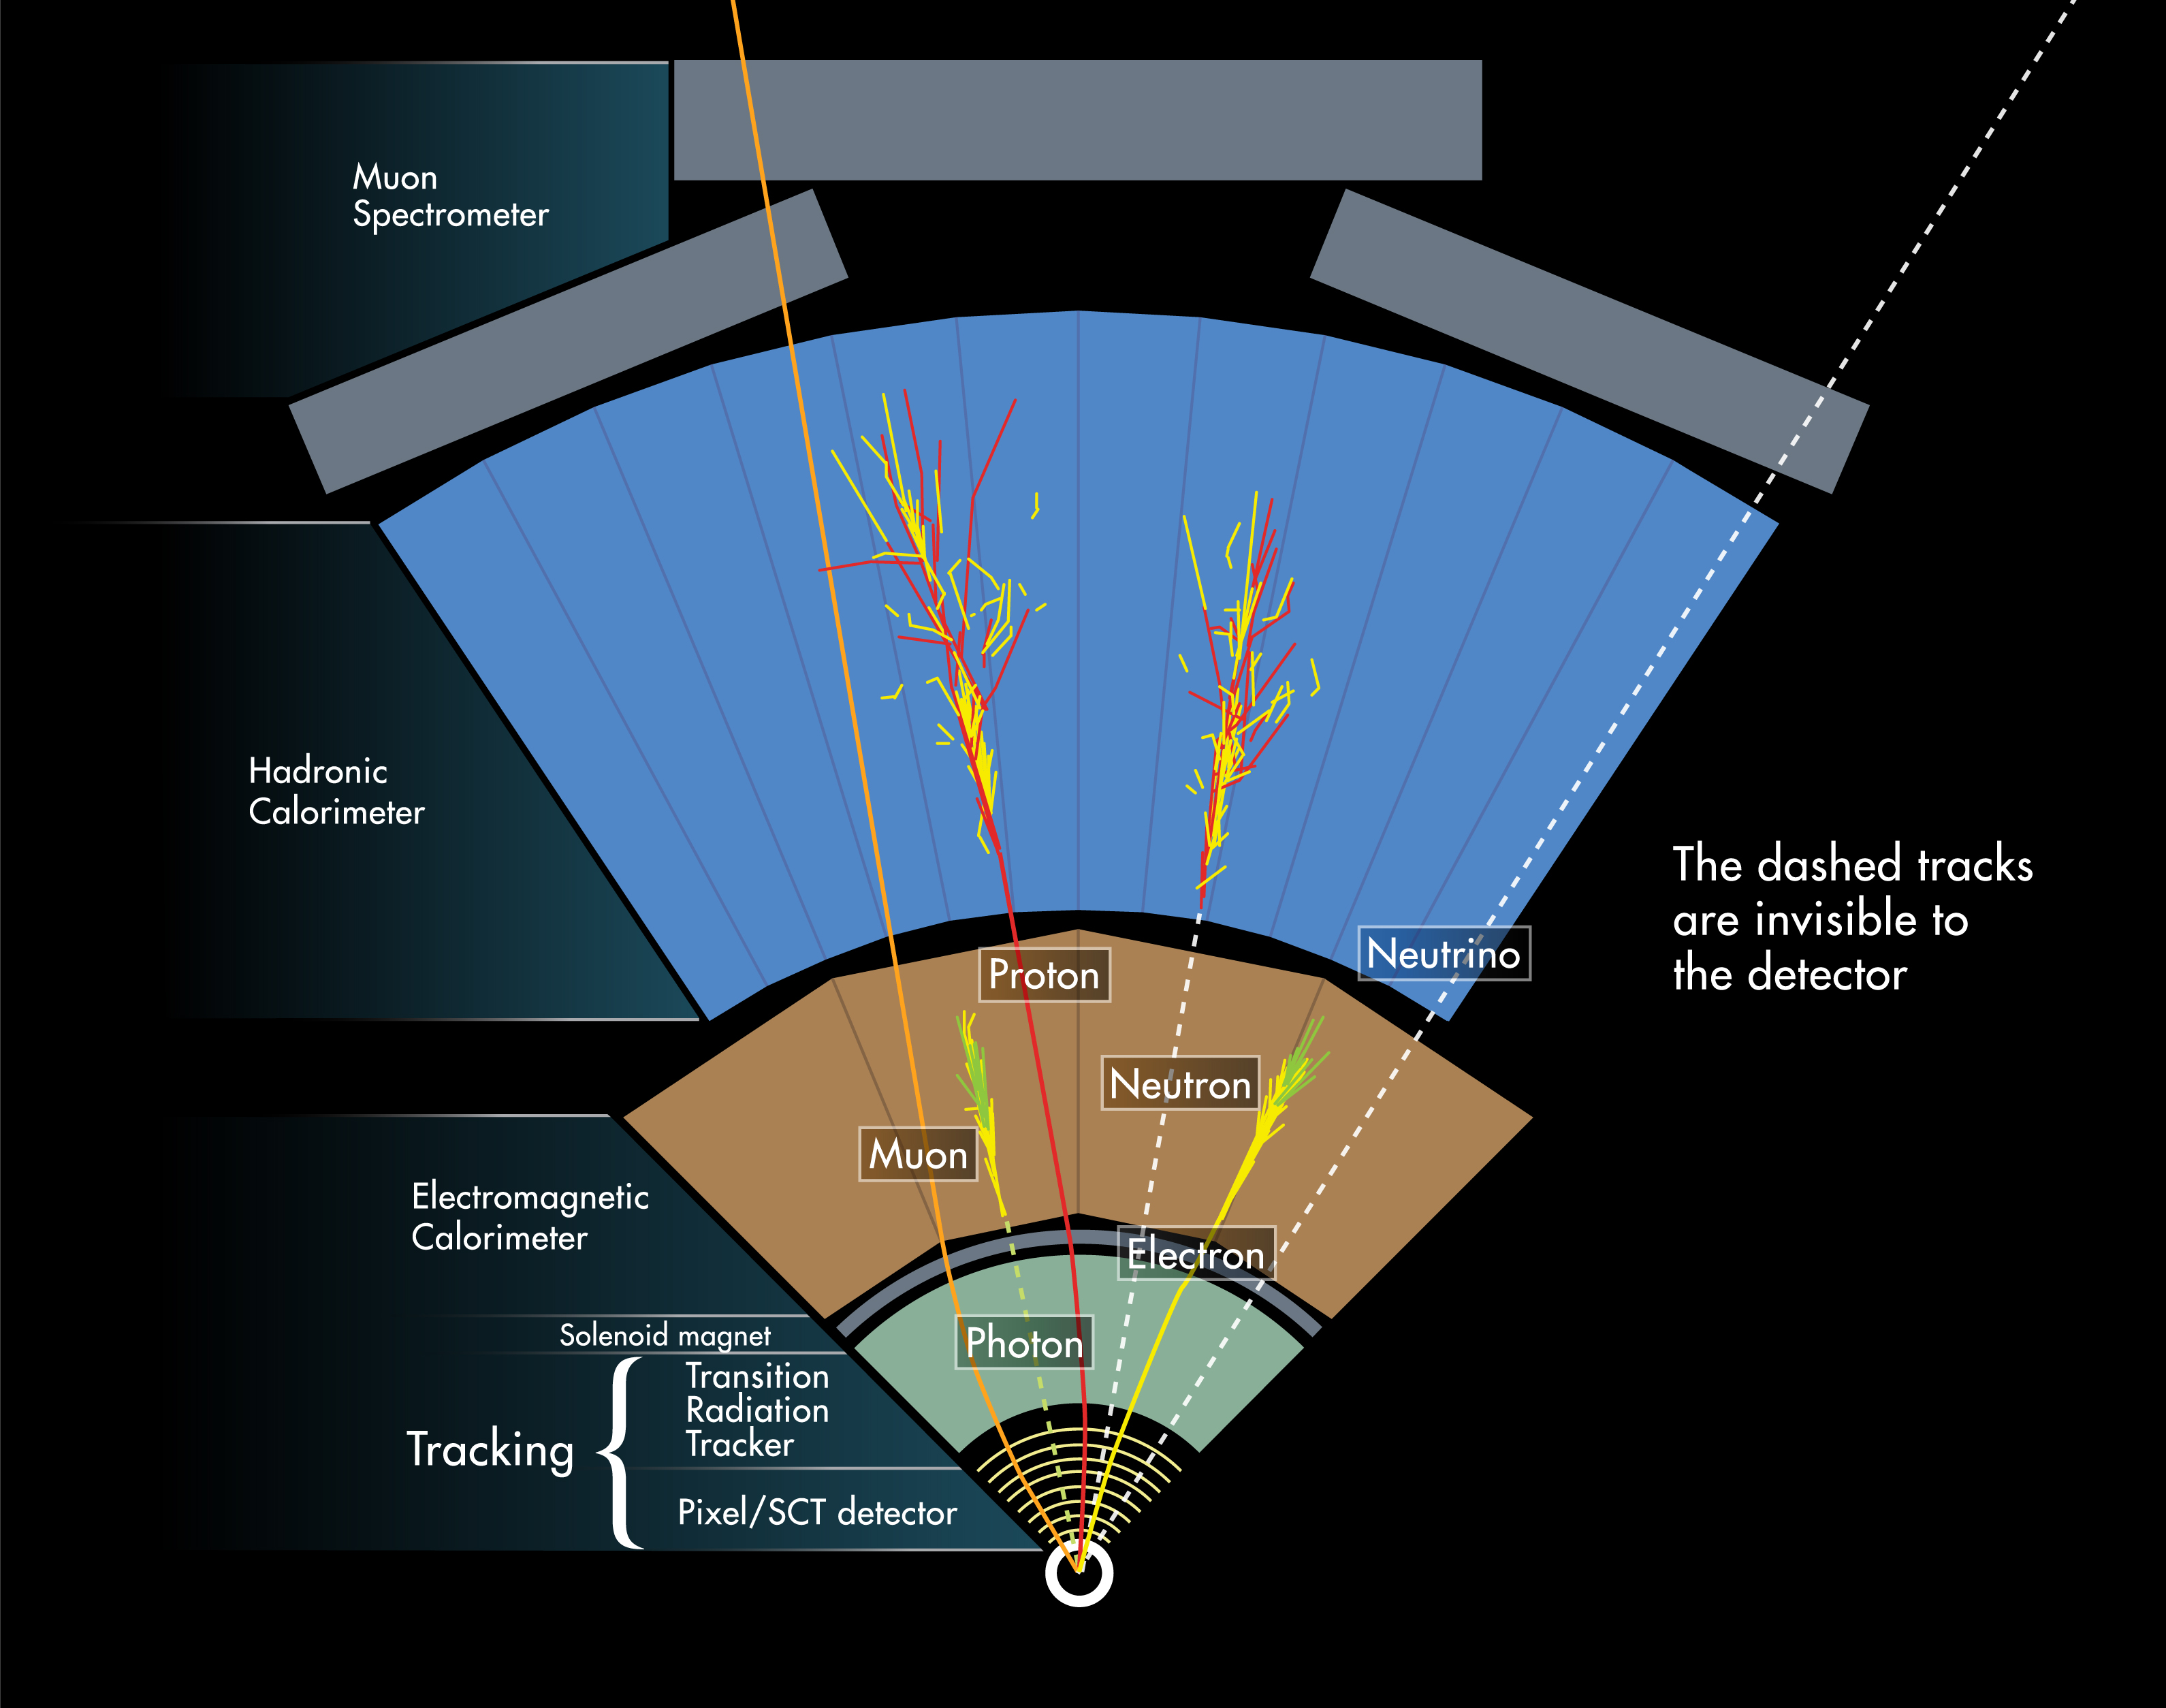
\includegraphics[scale=0.6]{figs/ch4/ATLAS-tracks.jpg}
    \caption{ Planar slice of the ATLAS detector showing different energy deposits of several physics objects \cite{atlas-detects}.}
\label{fig:4.1}
\end{figure}

\section{Track and Vertex Reconstruction}\label{sec:track-reco}

Almost all physics objects detected by \gls{atlas} deposit small amounts of energy within the \gls{id} sensors, each \textit{hit} is then used to reconstruct the object's 
track(s). Tracks are seeded by groups of three, one from the \gls{ibl}, another from the pixel detector and lastly the \gls{sct} \cite{track-reco}. Within the pixel and \gls{sct}
detectors, the track association begins with clustering raw measurements. A connected component analysis (\gls{cca}) \cite{cca} groups pixels and strip detectors together that share
a common edge or corner if energy has deposited on them above a certain threshold. These combined clusters are then referred to as \textit{space-points}. The average size of a
pixel cluster is about 2 pixels in the \textit{r}-$\phi$ plane and 1 to 3 pixels in the longitudinal direction with increasing η. Clusters from single charged particles are 
\textit{single-particle} clusters, clusters from multiple charged particles are referred to as \textit{merged} clusters and clusters from multiple tracks that are not 
compatible are called \textit{shared} clusters. A Kalman filter \cite{kalman} is applied to these \textit{merged} 
clusters to maximize track purity for objects of interest. Particles often share a hit, in this case a quality score is assigned to each track candidate. The score is 
determined by the number of \gls{id} layers with a hit, a track fit $\chi^{\textrm{2}}$ and the logarithm of the track momentum to suppress low $\textit{\textit{p}}_{\textrm{T}}$ 
track objects \cite{track-reco,newt}. For clusters assigned to multiple tracks in the merged clusters category, an ambiguity solver is applied. For the track selection criteria,
a track cannot be associated to no more than two shared clusters, cannot be over $\textit{\textit{p}}_{\textrm{T}} > \textrm{400 MeV}$ and $|\textrm{η}| < \textrm{2.5}$.
Using the hits in the \gls{trt}, the final track candidates are mapped out and a final selection occurs through track fitting. 
\par
Through the multiple \gls{pp} collisions in a bunch crossing, there is typically a single collision that yields objects of interest, this is called the hard-scatter. 
The main vertex of the hard-scatter and the secondary vertices from its decay products are mapped through the tracking procedure by applying track criteria. Multiple vertices
are found on the \textit{z}-axis from luminous peaks, called seed vertices. Here is where the track algorithm and its criteria are applied to find the primary vertex 
of the hard-scatter.

\section{Electrons}\label{sec:ele-reco}

Electrons are reconstructed using the energy deposits within the \gls{ecal} and tracks within the \gls{id}. The reconstruction comes in several steps. The first is combining the 
energy clusters within the \gls{ecal} into \gls{em}-topo clusters. Tracks are then matched to these clusters, creating superclusters. Electrons are then defined from these 
superclusters \cite{ele-reco}. 
\par
Proto-clusters are first defined within the \gls{ecal} and \gls{hcal} using a set of noise thresholds to discriminate from background noise. The clusters found in the \gls{hcal}
are not used in the electron reconstruction process, but are used to reduce background noise from pile-up. The cell clusters are required to 
have a significance $|\zeta^{\textrm{EM}}_{\textrm{cell}}| \ge \textrm{4}$ as defined in Eq. \ref{eq:4.1} \cite{ele-reco}:
%
\begin{equation}\label{eq:4.1}
    \zeta^{\textrm{EM}}_{\textrm{cell}} = \frac{\textrm{\textit{E}}^{\textrm{EM}}_{\textrm{cell}}}{\sigma^{\textrm{EM}}_{\textrm{noise,cell}}} 
\tag{4.1}
\end{equation}
%
$\textrm{\textit{E}}^{\textrm{EM}}_{\textrm{cell}}$ is the cell energy deposition and $\sigma^{\textrm{EM}}_{\textrm{noise,cell}}$ is the expected cell noise. This noise is 
the known electronics noise and an estimate of the pile-up noise corresponding to the instantaneous luminosity of Run 2. The algorithm then iterates through these clusters,
ignoring the first of the \gls{ecal} in order to suppress noise. These proto-clusters are then paired with neighboring clusters with a significance of $|\zeta^{\textrm{EM}}_{\textrm{cell}}| \ge \textrm{2}$.
These neighbors are then used as seed clusters of the next iteration to further find neighboring cells within the cluster. Once all the neighboring clusters with
$|\zeta^{\textrm{EM}}_{\textrm{cell}}| \ge \textrm{2}$ are found, they are then merged into a larger cluster. Proto-clusters with more than two or more local energy maxima, 
they are split into separate clusters. A maxima is considered when it has $\textrm{\textit{E}}^{\textrm{EM}}_{\textrm{cell}} >$ 500 MeV and at least four neighbors with 
smaller signal.   
\par
Tracks are then matched to the proto-clusters using information from the \gls{id} as described in Section \ref{sec:track-reco} \cite{ele-reco-2015}. Electrons lose a significant portion of their energy 
within the \gls{id} compared to other charged particles. To ensure efficiency in electron reconstruction, a loose track association criteria is applied. The conditions are 
$|\textrm{η}_{\textrm{track}} - \textrm{η}_{\textrm{cluster}}| <$ 0.05 and $-\textrm{0.10} < \textrm{\textit{q}}(\phi_{\textrm{track}} - \phi_{\textrm{cluster}}) <$ 0.05 where 
\textit{q} refers to the charge of the track. An ordering is applied to cases when multiple tracks are matched to a single cluster. Tracks found in the pixel detector are the most 
preferred, then tracks within the \gls{sct} with none in the pixel detector. Then the best $∆\mathrm{\textrm{R}}$ between the tracks and the cluster chosen. The track with the best score 
is then matched to the \gls{ecal} cluster and is used in the further steps of electron reconstruction.
\par
Superclusters are then defined from these chosen \gls{em} topo-clusters. The seeds chosen to form the superclusters are selected by requiring 
$\textit{E}_{\textrm{T}} = \sqrt{\textrm{\textit{m}}^{\textrm{2}}+\textit{\textit{p}}_{\textrm{T}}^{\textrm{2}}} \ge$ 1 GeV and matched track fulfilling quality criteria.
These superclusters are then extended by adding topo-clusters within $∆\textrm{η} \times ∆\phi =$ 0.075 $\times$ 0.125, these are considered \textit{satellite} clusters 
and are assumed to be secondary \gls{em} showers from the initial electron or photon. But for electrons, this distance is extended to $∆\textrm{η} \times ∆\phi =$ 0.125 $\times$ 0.3
 and the seed and the adjacent topo-cluster must share a matched track. These steps rely heavily on tracking information to discriminate between radiative photons or low energy 
 electrons from pile-up or noise. 
 \par
Once the superclusters are built, an initial energy calibration and position correction are applied to them. Tracks are matched to these supercluster while conversion vertices 
are matched to photons since they do not leave tracks within the \gls{id}. There are events with clear cut identification of electrons and photons, i.e., superclusters with 
defined tracks (electrons) and superclusters with no defined tracks (photons). But there are cases when there is ambiguity between both objects, when this occurs a classification 
process is applied to determine the type of object. The initial suepercluster calibration occurs before the track matching and relies on energy calibrations of the
electrons and photons to simulations \cite{ele-cali}. This process is referred to as energy scale calibration. The energy resolution of electrons found in data are used 
to calibrate simulations of $\textrm{\textit{Z}} \rightarrow \textrm{\textit{ee}}$ events. These simulated events are then used to derive the energy scale and resolution calibration 
factors. The invariant mass of two electrons in data and within these simulated events after the energy resolution is applied can be found in Figure \ref{fig:4.2} with good agreement.

\begin{figure}[h]
    \centering
    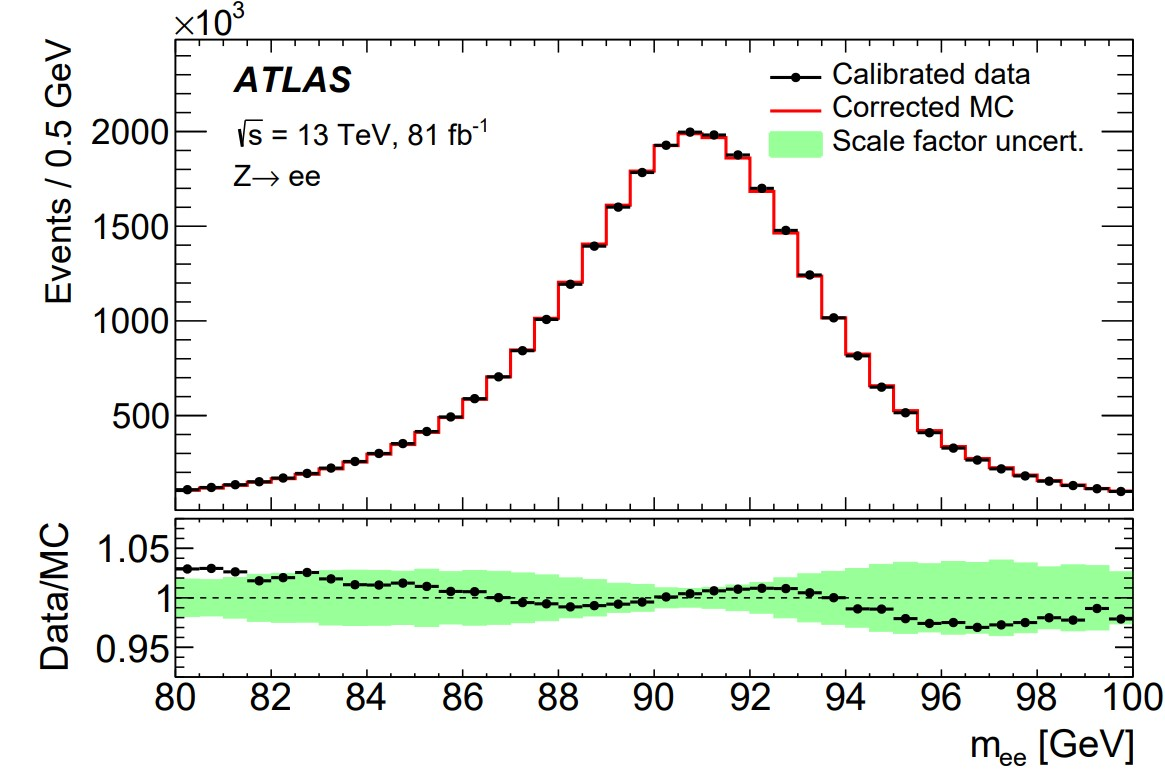
\includegraphics[scale=0.38]{figs/ch4/JES-ele.jpg}
    \caption{ Comparisons of simulated events and data after calibration and resolution corrections applied for electrons \cite{ele-reco}.}
\label{fig:4.2}
\end{figure}

\section{Muons}\label{sec:muon-reco}

Muons deposit little energy as it transverses the \gls{atlas} detector, thus its reconstruction relies heavily on associated tracks left within the \gls{id} and the (\gls{ms}) 
along with characteristic energy deposits in the calorimeters. The track reconstruction is for the \gls{ms} is independent of the track reconstruction in the \gls{id} as described 
in section \ref{sec:track-reco}, though the reconstructed muon depends on both \cite{muon-reco}.
\par  
Tracks within the \gls{ms} are identified as short straight-line local segments reconstructed from hits in individual stations. These segments are identified through a process 
known as a Hough transform \cite{Hough}. These segments are combined into preliminary track candidates using a loose constraint of the impact parameter (\gls{ip}, discussed in Section~\ref{sec:ip-algo}) and a parabolic trajectory that includes the first-order approximation of the track bending due to the magnetic field. These calculations are combined with precision 
information of a second coordinate from the trigger detectors, creating a three-dimensional track. This track then has a global fit $\chi^{\textrm{2}}$ fit of the muon trajectory
through the magnetic fields within the \gls{ms}. The hits that are not contained within the fit of the muon trajectory are removed. Hits are added onto the fit trajectory that 
were not originally there, from these aligned hits, another $\chi^{\textrm{2}}$ fit is applied. Less quality tracks are removed when they share a fraction of hits with a high 
quality track in order to resolve ambiguities. The final track is then re-fitted with a \gls{ip} constraint that takes into account the energy loss in the calorimeters and 
an extrapolated trajectory back to the beam line \cite{muon-reco}. 
\par
This fitting procedure using hits within the \gls{ms} and \gls{id} are applied in several different reconstruction strategies.

\begin{itemize}
    \item Combined (CB): Combined muons are identified by matching \gls{ms} to \gls{id} tracks and applying a combined fit as previously discussed. For muons with 
    $|\textrm{η}| >$ 2.5, \gls{ms} track segments are combined with hits from the pixel detector and \gls{sct} detector. These boosted muons are considered a subset called 
    silicon-associated forward (SiF) muons
    \item Inside-Out Combined (IO): Muons reconstructed using this method uses an algorithm which extrapolates the \gls{id} hits to the \gls{ms} and searches for at minimum three
    loosely associated hits. Between these loosely associated hits, the small energy loss within the calorimeters are used to verify. A Combined track fit is then applied.
    \item Muon-Spectrometer Extrapolated (ME): These are muon tracks within the \gls{ms} but cannot be associated with any hits within the \gls{id}. If this is the case, the tracks
    are extrapolated all the way back to the beam line. Because of this, this extends the \gls{ms} coverage to $|\textrm{η}| =$ 2.7.  
    \item Segment-Tagged (ST): ST requires at least one \gls{ms} segment to be associated with an extrapolated \gls{id} track. 
    \item Calorimeter-Tagged {CT}: These muons are identified by taking the extrapolated tracks in the \gls{id} through the calorimeters. Muons deposit minimum-ionizing 
    energy in the calorimeters. If CT was used to identify the muon, the parameters are obtained directly through the track fit. 
\end{itemize}

After reconstruction, high quality muon candidates are then selected using criteria utilizing the sub-detectors. The set of requirements on the identified muons given its type as 
stated above is referred to as its selection \textit{working point} (\gls{wp}). The definition of muon \gls{wp}s depends on the type of analysis involving final state muons. 
The standard \gls{wp}s designed to cover needs of most analyses vary in increasing purity and decreasing muon tagging efficiency. The \gls{wp}s are \textit{loose}, \textit{medium},
and \textit{tight}. Here, muons passing the \textit{medium} \gls{wp} is a subset of the \textit{loose} \gls{wp}. These were defined to help optimize different physics analyses. 
The \textit{medium} \gls{wp} is suitable for most general analyses where the \textit{loose} was optimized for Higgs boson decays into a four muon final state \cite{muon-reco}.
\par
Muon correction factors are obtained through simulation events of $\textrm{\textit{Z}} \rightarrow \textrm{\textit{µµ}}$ and $\textrm{\textit{J}}/\psi \rightarrow \textrm{\textit{µµ}}$. The momenta
in the simulation are corrected to those obtained through data. Multiplicative correction factors are obtained to correct for reconstruction, identification, and isolation 
efficiencies of simulation to data. 

\section{Jets}

Most \gls{pp} collision events result is quarks or gluons. Due to quark confinement within \gls{qcd}, these partons cannot exist independently and undergo 
a process called hadronization, resulting in color-less cone-like sprays of hadrons. The cones, or jets, are reconstructed using tracks from the \gls{id} and energy 
depositions with the \gls{hcal}. The energy deposition and correlated tracks undergo the same topo-cluster algorithm defined for electrons that was discussed in section \ref{sec:ele-reco}.
Two types of jets are defined depending on the radii of the cone. There are small-radius (\gls{sr}) jets and large-radius (\gls{lr}) jets.
Figure \ref{fig:4.1} shows two jets deposited in the blue colored \gls{hcal}, one from a proton, the other from a neutron. 

\subsection{Jet Definition}\label{sec:jet-def}

Since quarks cannot exist independently due to quark confinement, jet reconstruction must rely on complex algorithms exploiting jet kinematics in order to identify the 
initial quark. The jet reconstruction algorithm must allow for reliable comparison to theory and experiment \cite{antikt}. In order to identify jets associated to the hard-scatter 
event, the jet algorithm must be insensitive to soft (low momentum) and collinear (low angle) hadrons. 
\par
The current \gls{atlas} standard of such algorithms is called the anti-$\textrm{\textit{k}}_{\textrm{T}}$ algorithm \cite{antikt}. This process identifies hadronic energy depositions as inputs and forms 
jets through sets of criteria. First it chooses some object \textit{i} in a list of objects, calculates the distance $\textrm{d}_{\textrm{\textit{i}}\textrm{\textit{j}}}$
between two objects within the list and then it calculates the distance $\textrm{d}_{\textrm{\textit{i}}\textrm{\textit{B}}}$ between object \textit{i} and the beam (\textit{B}).
This is shown in Eq. \ref{eq:4.2} .
%
\begin{equation}\label{eq:4.2}
\begin{split}
    \textrm{d}_{\textrm{\textit{i}}\textrm{\textit{j}}} = \textrm{min}(\textrm{\textit{p}}^{\textrm{2\textit{p}}}_{\textrm{T,\textit{i}}},\textrm{\textit{p}}^{\textrm{2\textit{p}}}_{\textrm{T,\textit{j}}}) \frac{∆^{\textrm{2}}_{\textrm{\textit{i,j}}}}{\textrm{R}^{\textrm{2}}} \ ,\\
    \textrm{d}_{\textrm{\textit{i}}\textrm{\textit{B}}} = \textrm{\textit{p}}^{\textrm{2p}}_{\textrm{\textit{ti}}}
\end{split}
\tag{4.2}
\end{equation}
%
Where:
%
\begin{equation}\label{eq:4.3}
    ∆^{\textrm{2}}_{\textrm{\textit{i,j}}} = (\textrm{\textit{y}}_{\textrm{\textit{i}}}-\textrm{\textit{y}}_{\textrm{\textit{j}}})^{\textrm{2}} + (\phi_{\textrm{\textit{i}}}-\phi_{\textrm{\textit{j}}})^{\textrm{2}}
\tag{4.3}
\end{equation}
%
and $\textrm{\textit{p}}_{\textrm{T,\textit{i}}}$, \textit{y}$_{\textrm{\textit{i}}}$ and $\phi_{\textrm{\textit{i}}}$ are respectively the momentum, rapidity, and azimuthal 
angle of object \textit{i}. The radius of the jet cone is denoted as \textit{R} and the parameter \textit{p} is to help govern relative power of the energy. For the anti-$\textrm{\textit{k}}_{\textrm{T}}$ 
algorithm the parameter \textit{p} is set to $-$1. The algorithm then finds the minimum between $\textrm{d}_{\textrm{\textit{i}}\textrm{\textit{j}}}$ and $\textrm{d}_{\textrm{\textit{i}}\textrm{\textit{B}}}$.
if the minimum is the distance between the two objects \textit{i} and \textit{j}, then the four momenta of the objects are combined. Whereas, if the  $\textrm{d}_{\textrm{\textit{i}}\textrm{\textit{B}}}$
is the minimum, object \textit{i} is regarded as a jet. This procedure continues as long as objects remain on the list. 
\par
Due to the inverse dependence on $\textrm{\textit{p}}_{\textrm{T}}$, soft objects are combined with close-by hard objects (high momentum) before two soft objects are combined \cite{antikt}.
Jets tend to have a conical shape around the hardest object \textit{i} when using anti-$\textrm{\textit{k}}_{\textrm{T}}$ algorithm for reconstruction. However, when two hard objects are within a relative 
distance of $∆(\textit{i},\textit{j}) \le \textrm{2}\textrm{R}$ of one another, it's difficult to differentiate the jet substructure of either jet. If the two hard objects are within 
$\textrm{R} < ∆(\textit{i},\textit{j}) \le \textrm{2}\textrm{R}$ then the anti-$\textrm{\textit{k}}_{\textrm{T}}$ algorithm forms two jets. The shapes of these two hard object jets depends on the transverse 
momenta of both, ending in one shape to be conical where the other is partially cone-shaped. If two hard objects are found within $∆(\textit{i},\textit{j}) < \textrm{R}$, a single 
jet is formed and the shape is defined by the momenta of the two hard objects. If the momenta are similar, the jet is can be constructed of two cones (with radii lower than R)
inside one larger cone. Figure \ref{fig:antikt} shows several jets classified using the anti-$\textrm{\textit{k}}_{\textrm{T}}$ algorithm, along with a large-radius jet containing two small-radius jets. 
\par 
Two types of jets are presented in this thesis. Both are the previously stated \gls{sr} and \gls{lr} jets. The cone radii for these types correspond to R = 0.4 for \gls{sr} and 
R = 1.0 for \gls{lr}. More about these two types are explained in the following sections.

\begin{figure}[H]
    \centering
    \subfloat[\centering ]{{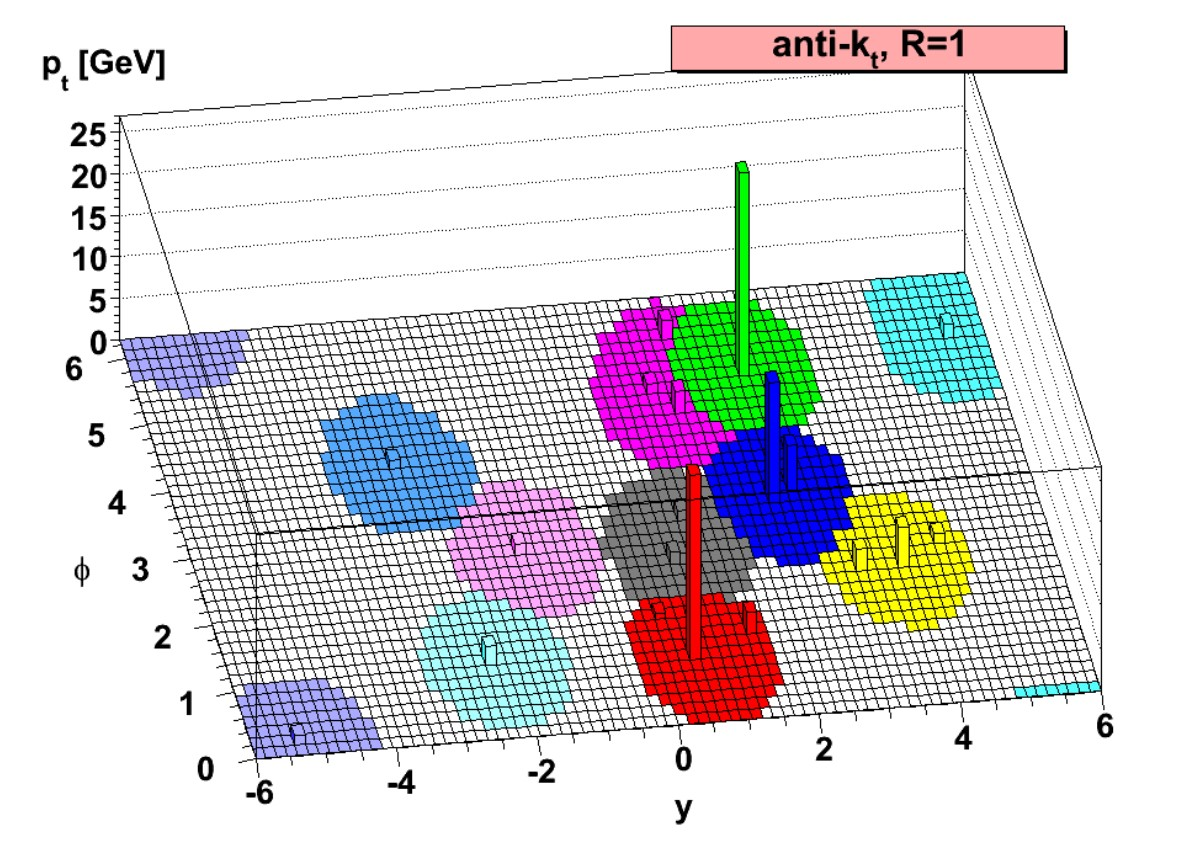
\includegraphics[scale=0.25]{figs/ch4/antikt.jpg}}}%
    \qquad
    \subfloat[\centering ]{{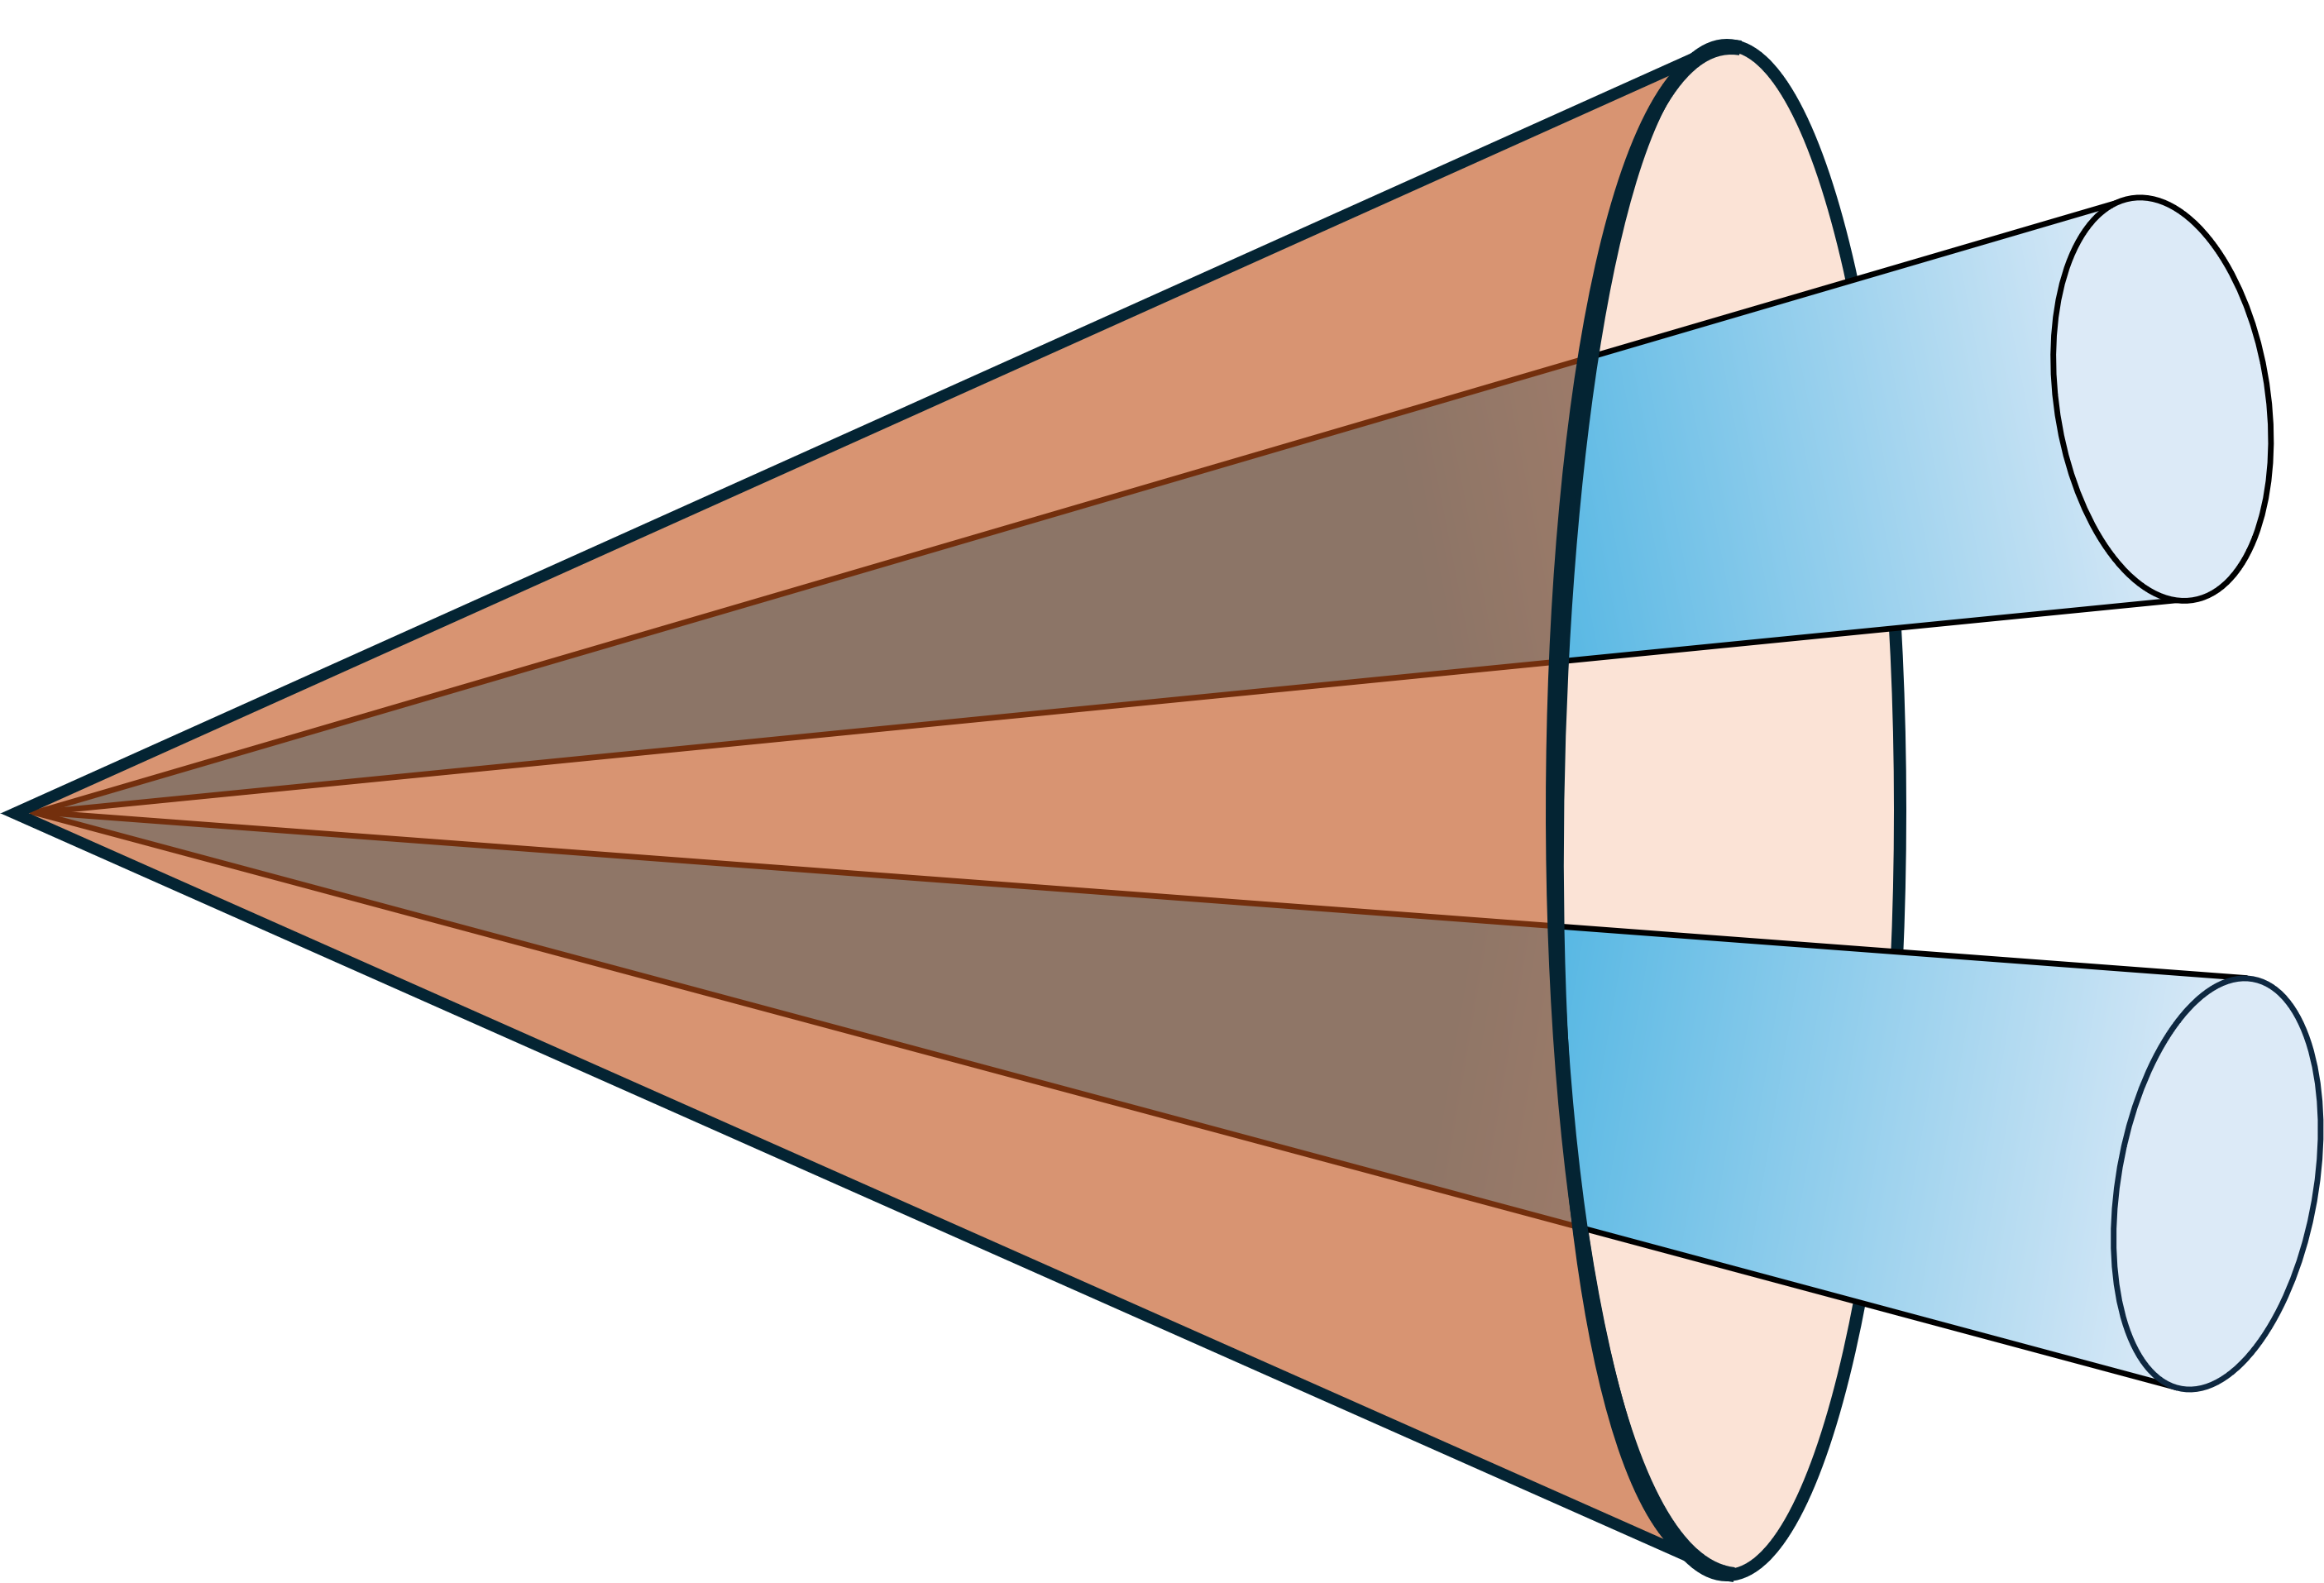
\includegraphics[scale=0.25]{figs/ch4/LR_jet.png}}}%
    \caption{(a) Shapes and the substructures of jets formed using the anti-$\textrm{\textit{k}}_{\textrm{T}}$ algorithm in the $\phi$ -\textit{y} plane \cite{antikt}. The height in the \textit{z}-axis corresponds to the momentum of the hard objects. 
    Figure (b) Substructure of a large-radius jet containing two small-radius jets of similar $\textrm{\textit{p}}_{\textrm{T}}$ }
    \label{fig:antikt}
  \end{figure}

\subsection{Small Radius Jets}\label{sec:small-R}

There are several approaches to defining a \gls{sr} jet. The jets used in this thesis, and are currently ATLAS standard objects, are called \textit{particle flow} or \textit{PFlow}.
PFlow objects are the building blocks of PFlow jets. These objects are clusters within the calorimeters and their constituted tracks \cite{pflow,jes}. Proto-clusters as previously defined in 
Section \ref{sec:ele-reco} are standard PFlow objects \cite{ele-reco}. The energy depositions in the \gls{ecal} and \gls{hcal} used to form these proto-clusters are calibrated 
to the \gls{em} scale in order to get a correct measurement of the showers \cite{jes}. A weighted mean of the cluster cells is calculated. This value is used to assign 
$\phi$ and η coordinates, as well as the energy deposited \cite{topo-cluster}. From here, it's assumed this cluster points to the origin of the coordinate system of the detector.
The proto-cluster is taken as a particle of zero mass and has its four-momentum calculated \cite{topo-cluster}. All the weighted clusters are assumed to be produced from objects
originating from the hard-scatter, an origin correction is then applied \cite{jes}, altering the momentum values to point towards the primary vertex. 
\par
\gls{sr} are defined as these corrected calorimeter proto-clusters with their associated tracks. A previously used jet class called \textit{EMTopo} jets was used. But this class 
only utilized the proto-cluster energy depositions and didn't use the track information from the \gls{id}. The \gls{id} has very precise momentum resolution for low 
momentum tracks, combining these to the calorimeter energy depositions greatly increased jet energy resolution in low energy jets. Giving jets improvements in its energy and 
direction while also lessening dependence on the number of pile-up interactions \cite{jes}.
\par
Tracks defined as PFlow objects but adhere to a tighter criteria than previous cases. A crucial energy subtraction procedure is performed to prevent double counting of energy 
contributions of charged particles leaving tracks in the \gls{id} and energy deposited in the calorimeters \cite{pflow,jes}. Energy that can be associated to a PFlow track is 
subtracted out of the clusters. A distance metric is applied between the center of the cluster and its possibly associated track as defined in Eq. \ref{eq:4.4}.

\begin{equation}\label{eq:4.4}
    ∆\textit{R'} = \sqrt{\left(\frac{∆\phi}{\sigma_{\phi}}\right)^{\textrm{2}}+\left(\frac{∆\textrm{η}}{\sigma_{\textrm{η}}}\right)^{\textrm{2}}}
\tag{4.4}
\end{equation}

Where $\sigma_{\phi}$ and $\sigma_{\textrm{η}}$ represent the angular topo-cluster width, calculated as the standard deviation of the displacements, $\phi$ and $\textrm{η}$, of the 
cluster cell center \cite{pflow}. Taking the smallest $∆\textit{R'}$ to be matched to a track succeeds in virtually 
all particles with $\textrm{\textit{p}}_{\textrm{T}} >$ 5 GeV. If no topo-cluster is found in a cone with $∆\textit{R'}$ = 1.64, it is assumed the particle did not form a cluster 
in the calorimeter and no momentum procedure is applied \cite{pflow}. 
\par
For each track matched to a cluster, the energy deposited by the particle is evaluated using simulated events. After a charged particle traversed the \gls{id}, it is possible that 
it would leave more than one topo-cluster in the calorimeters. If this is the case and the topo-cluster has energy below the expected amount, clusters within $∆\textit{R'}$ = 0.2
of the track are combined. Once the track-to-cluster matching occurs, energy is subtracted from the calorimeter topo-clusters. Energy deposits around the subtracted clusters 
that are found within reasonable shower fluctuations are also subtracted. The final PFlow object is considered the total subtracted energy from the calorimeter and the matched 
tracks that are compatible to the primary vertex. 

\subsection{Large Radius Jets}

As the momentum of massive particles (e.g. W, Z, Higgs, or the top-quark) increases, they become more Lorentz boosted. When these particles decay, their decay products are also 
highly Lorentz boosted, collimating them in a single direction. It is advantageous, in this case, to adjust the radius parameter \textit{R} from the small-R jets and to increase it in 
order to contain all the collimated decay products. The parameter for large-R jets is increased to \textit{R} = 1.0. By increasing the radius parameter, multi-pronged jet 
substructure from two-body or three-body decays is much more effectively captured \cite{LR-jets}.  
\par
The reconstruction of \gls{lr} jets is complicated due to the presence of soft radiation, i.e. energy deposition from underlying pile-up and uncorrelated jets. These degrade the 
reconstruction performance, \gls{lr} jet mass resolution and other sub-structure quantities. \gls{lr} jets are typically reconstructed using the anti-$\textrm{\textit{k}}_{\textrm{T}}$ algorithm and historically 
have been based solely on calorimeter energy measurements which have provided excellent energy resolution. By only using energy depositions in the calorimeters, it is difficult 
to reconstruct separate particles within the \gls{lr} jet radius of \textit{R} = 1.0, especially where the calorimeter resolution is coarse. It is important to distinguish the 
\gls{lr} jet sub-structure and therefore several PFlow algorithms are implemented to extract this information. A variant of the PFlow algorithm called Track-CaloClusters (\gls{tcc})
was designed to reconstruct jet sub-structure even at the highest transverse momenta. The structures identified using \gls{tcc}s and PFlow is called Unified Flow Objects, or 
\gls{ufo}s. Pile-up mitigation techniques are also implemented such as constituent subtraction, Voroni subtraction, SoftKiller, and pile-up per particle identification (PUPPI).
\par
A trimming procedure is enacted inside the \gls{lr} jet to reduce the sub-structure constituents that may be related to soft radiation. Several criteria are implemented in this 
trimming procedure, such as using the ratio of the $\textrm{\textit{p}}_{\textrm{T}}$ of the sub-jet constituents. This trimming procedure uses the $\textrm{\textit{k}}_{\textrm{t}}$ algorithm to create sub-jets 
inside the large radius, creating jet objects with a radius parameter $\textrm{\textit{R}}_{\textrm{sub}}$. Any sub-jets with $\textrm{\textit{p}}_{\textrm{T}_{\textrm{i}}}/\textrm{\textit{p}}_{\textrm{T}}^{\textrm{jet}} < \textrm{f}_{\textrm{cut}}$.
Where $\textrm{\textit{p}}_{\textrm{T}_{\textrm{i}}}$ is the transverse momentum of the $\textrm{i}^{\textit{\textrm{th}}}$ sub-jet, and $\textrm{f}_{\textrm{cut}}$ is the cut parameter.
The optimized parameters used for this trimming procedure are $\textrm{f}_{\textrm{cut}}$ = 0.3 and $\textrm{\textit{R}}_{\textrm{sub}}$ = 0.2. Figure \ref{fig:trim} shows a diagram of a trimmed jet.

\begin{figure}[h]
    \centering
    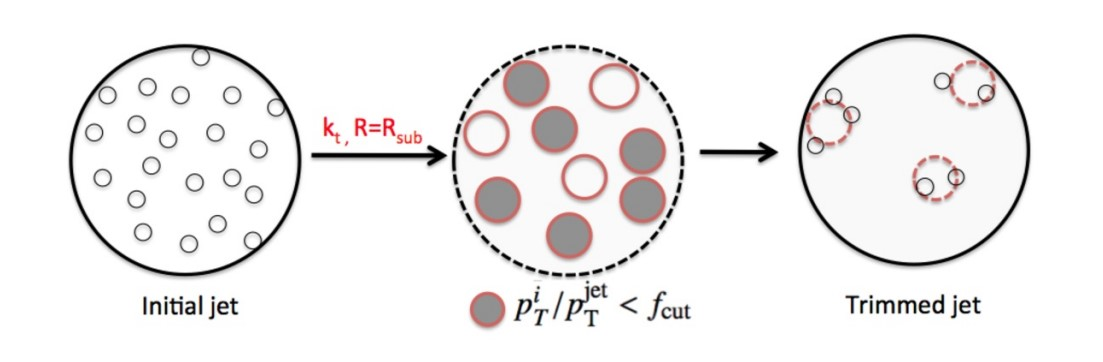
\includegraphics[scale=0.50]{figs/ch4/LR_trim.jpg}
    \caption{ Diagram illustrating the LR jet trimming procedure \cite{LR-jets-opt}.}
\label{fig:trim}
\end{figure}

Mass is then assigned to each trimmed jet according to their four-momentum squared. To improve trimmed jet mass resolution for high-$\textrm{\textit{p}}_{\textrm{T}}$ \gls{lr} jets,
an additional mass ($\textrm{\textit{m}}_{\textrm{TA}}$) is added based on tracks associated with the jet, calculated using Eq. \ref{eq:4.5}. Tracks are associated to sub-jets through a technique called ghost-association. A 
pseudo-particle is reconstructed for each track, having the same coordinates and direction as the track. These pseudo-particles are input into the anti-$\textrm{\textit{k}}_{\textrm{T}}$ algorithm along with 
the energy clusters in the calorimeter. These pseudo-particles are very soft and therefore do not alter the resulting sub-jets. A track is associated to a sub-jet if a corresponding 
pseudo-particle is clustered into the sub-jet. This technique of using ghost-association allows for irregular shaped jets, resulting in an occasional non-cone shaped jet. 

\begin{equation}\label{eq:4.5}
    \textrm{\textit{m}}_{\textrm{TA}} = \frac{\textrm{\textit{p}}_{\textrm{T}}^{\textrm{jet}}}{\textrm{\textit{p}}_{\textrm{T}}^{\textrm{track}}}\textrm{\textit{m}}_{\textrm{track}}
\tag{4.5}
\end{equation}

Where $\textrm{\textit{p}}_{\textrm{T}}^{\textrm{jet}}$ is the transverse momentum of the \gls{lr} jet, $\textrm{\textit{p}}_{\textrm{T}}^{\textrm{track}}$ is the transverse 
momenta of a trimmed anti-$\textrm{\textit{k}}_{\textrm{T}}$ \gls{lr} jet formed from the tracks associated to the jet and $\textrm{m}_{\textrm{track}}$ is the mass of the track jet. The $\textrm{m}_{\textrm{track}}$
is multiplied by this ratio to include energy from the track of the sub-jet. To further improve the jet mass resolution, a combined mass is calculated from a weighted average of the 
two masses as shown in Eq. \ref{eq:4.6}
%
\begin{equation}\label{eq:4.6}
    \textrm{\textit{m}}_{\textrm{comb}} = \textrm{\textit{a}} \cdot \textrm{\textit{m}}_{\textrm{jet}} + \textrm{\textit{b}} \cdot \textrm{\textit{m}}_{\textrm{TA}}
\tag{4.6}
\end{equation}
%
The weights of \textit{a} and \textit{b} must satisfy \textit{a} $+$ \textit{b} = 1 and are derived from resolutions of $\textrm{\textit{m}}_{\textrm{jet}}$ and
$\textrm{\textit{m}}_{\textrm{TA}}$. The final calculated value of $\textrm{\textit{m}}_{\textrm{comb}}$ is the mass of the \gls{lr} jet.
\par
Energy and mass for the trimmed \gls{lr} jets are calibrated in data and simulation to equal values found at particle level in simulated di-jet events \cite{LR-jets-opt}. 
These calibrations are referred to as jet energy scale (\gls{jes}) and jet mass scale (\gls{jms}). The \gls{jes} is corrected first and subsequently the \gls{jms}. In-situ 
calibrations are taken to account for imperfect detector simulations are derived for \gls{jes}, \gls{jer}, and \gls{jms} \cite{LR-jets-cali}. These are performed on all three values of mass from Eq. \ref{eq:4.6}, 
$\textrm{\textit{m}}_{\textrm{jet}}$, $\textrm{\textit{m}}_{\textrm{TA}}$ and $\textrm{\textit{m}}_{\textrm{comb}}$

\subsection{PFlow Object Calibration}

The built PFlow objects are used as input into the anti-$\textrm{\textit{k}}_{\textrm{T}}$ algorithm as discussed in Section \ref{sec:jet-def} \cite{antikt} with \textit{R} = 0.4 to define \gls{sr} jets.
These jets undergo a multi-step calibration. The energy of a reconstructed jet is corrected to match the reconstructed jet at particle level \cite{jes}. This step is known as 
jet energy scale (\gls{jes}). 
\par
Pile-up particles produced in \gls{pp} collisions can deposit energy that may alter the kinematics of the defined \gls{sr} jet. These contributions are subtracted in the 
first step of the \gls{jes} calibration. The energy is compared to di-jet events at particle level from simulation, correcting the four-momentum vectors \cite{jes}.
The next step is referred to as the global sequential calibration (\gls{gsc}). This step corrects dependent parameters such as particles initiating a jet, shower fluctuations, 
and possible showers not detected by the calorimeters or caught in the muon spectrometer. These corrections are evaluated again by using simulated di-jet events.
The final step is to find additional correction factors to mitigate remaining discrepancies to jets from data. The corrections are called in-situ \gls{jes} calibration factors 
and are obtained by evaluating events that contain jets and well calibrated objects, such as electrons, muons or photons. Using momentum balance between these objects, correction 
factors and calculated and applied \cite{jes}. Systematic uncertainties associated with these correction factors arise from modeling in the simulation
\par 
The jet energy resolution (\gls{jer}) is also calibrated. The resolution of an object in the detector depends on background noise of the electronics and energy deposits from 
pile-up. The corrections are found comparing the \gls{jer} from simulated di-jet events to that of data. The correction factors are derived from these di-jet events and 
are applied by smearing the energy distribution to match that of data. Systematic uncertainties are obtained in this calibration step. 

\subsection{Jet Vertex Tagger}

Taggers are tools developed by the \gls{atlas} Flavor Tagging (\gls{ftag}) group to help identify which hadron flavor reconstructed jets originate from. 
The jet vertex tagger (\gls{jvt}) is a tagger used to help identify if tracks are associated to the primary vertex of the hard-scatter \cite{jvt}. There are many \gls{pp} collision that 
occur in a bunch crossing which is the reason for pile-up. So to correctly identify tracks of the collision of interest is crucial. The \gls{jvt} is a multivariate tagger 
algorithm that uses the jet $\textrm{\textit{p}}_{\textrm{T}}$ and its associated tracks. It uses the likelihood of the track being associated to a different collision vertex 
as a discriminating variable. This tagger is only used on jets within $|\textrm{η}| < $ 2.5, for any object that are more forward, a different algorithm is used called the 
forward jet vertex tagger (\gls{fjvt}) \cite{fjvt}.
\par
The \gls{jvt} and \gls{fjvt} efficiencies are measured in data and simulation \cite{jvt,fjvt}. These are determined through simulated events of $\textrm{\textit{Z}} \rightarrow \textrm{a} + \textrm{jets}$,
employing a tag and probe method. Scale factors are derived to correct for discrepancies in the efficiency measurements of data and simulation. 

\section{Heavy-Flavor Tagging}\label{sec:heavyFlavorTagging}

Identifying heavy flavors of quarks plays a crucial role in particle physics analyses. Many interesting physics analyses have b- or c-quarks in their final state. Such as the 
$\textrm{SH} \rightarrow b \bar{b} b \bar{b}$ final state which is discussed in the final part of this thesis.
Flavor tagging (\gls{ftag}) helps discriminate background processes from signal events. Therefore, this process has an important role in not just finding new physics, but also 
precision measurements. 
Since quarks undergo hadronization and cannot exist independently, the quarks themselves cannot be tagged, but rather a color neutral states, b- and c-hadrons. The b-hadrons 
have a lifetime of around 1.5 ps \cite{review-of-hep}, thus decaying after traversing the length of 2.5 mm when it has about 30 GeV. The b-hadron is also associated with a high decay multiplicity of 
an average of five charged particles. Figure \ref{fig:bjet-plots} (a) shows the charged particle decay count from a b-hadron ($\textrm{B}^{\textrm{0}}$), where (b) shows the $\textrm{\textit{p}}_{\textrm{T}}$
fraction the b-hadron carries within the jet which peaks at about 70\%. This results in another important property of a b-jet, it has a high semi-leptonic decay fraction. The typical 
b-jet looks like Figure \ref{fig:bjet-cartoon}. The b-hadron has a decay length L and is indicated by the red dotted line. This leads to a secondary vertex. The decay products from the secondary 
vertex may lead to a tertiary vertex, especially if it's a c-hadron. The displacement of the secondary vertex with respect to the primary vertex is given by a parameter called 
the decay length. The displacement of a track with respect to the primary vertex is parameterized with impact parameters (\gls{ip}s) denoted as $\textrm{d}_{\textrm{0}}$ in 
the figure. This $\textrm{d}_{\textrm{0}}$ \gls{ip} tends to be large for b-hadrons due to the long decay lifetime and large mass (5 GeV). 
\par

\begin{figure}[H]
    \centering
    \subfloat[\centering ]{{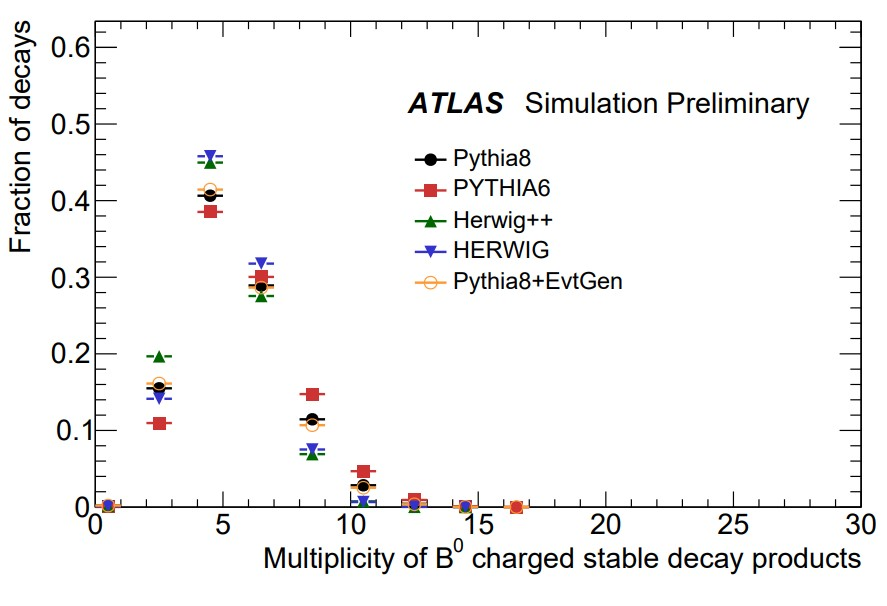
\includegraphics[scale=0.32]{figs/ch4/bjet-stable.jpg}}}%
    \qquad
    \subfloat[\centering ]{{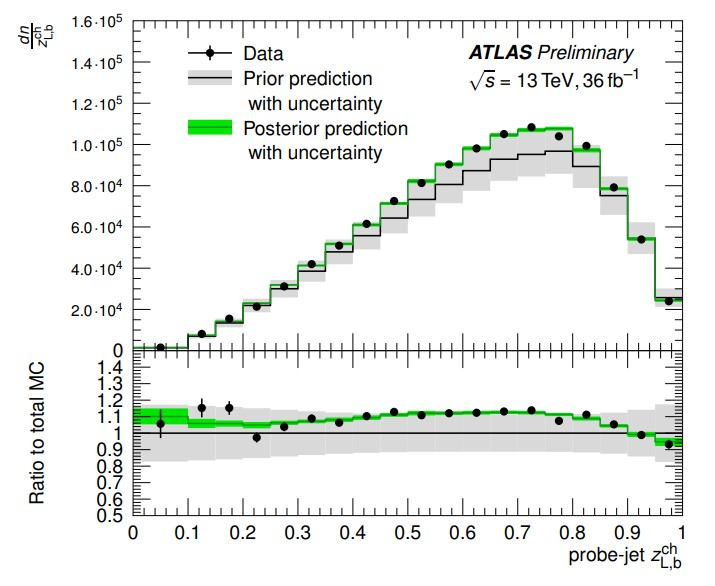
\includegraphics[scale=0.42]{figs/ch4/bjet-pt.jpg}}}%
    \caption{ (a) Decay multiplicity of the b-hadron $\textrm{d}_{\textrm{0}}$ into stable charged products with compared MC generators.
    (b) Fragmentation of b-hadron $\textrm{\textit{p}}_{\textrm{T}}$ }
\label{fig:bjet-plots}
\end{figure}

\begin{figure}[h]
    \centering
    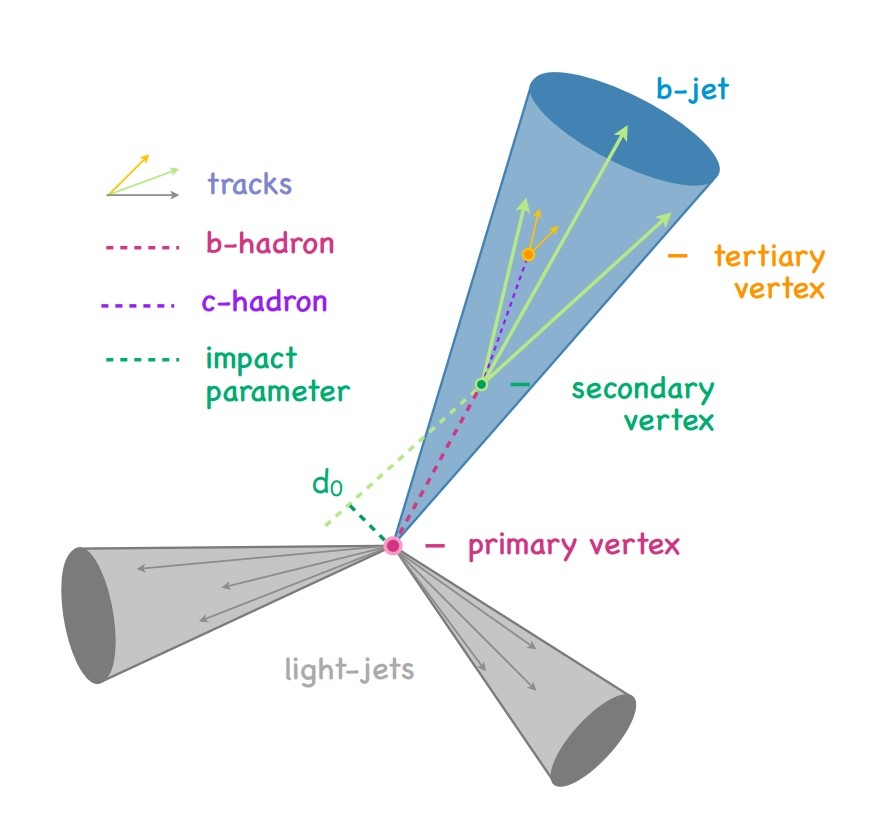
\includegraphics[scale=0.5]{figs/ch4/bjet-cartoon.jpg}
    \caption{ Diagram view of a b-jet with a first, second, and third vertex labeled.}
\label{fig:bjet-cartoon}
\end{figure}

C-hadrons tend to have less stable charged particle multiplicity, shorter decay lengths (resulting in a smaller $\textrm{d}_{\textrm{0}}$) and are lighter. This results in 
similar jet topologies, but not identical. Light-jets originate from lighter quarks which results in tracks being associated with the hadronization itself. These properties 
of c- and light-jets make them separable from b-jets. All these unique b-jet properties are targeted by \gls{ftag} tools developed to \textit{tag} a b-hadron. There are several 
b-tagging algorithms, all attempting to extract specific features of the b-hadron's information. These baseline algorithms can be categorized into three categories:
the \gls{ip} based algorithms called Impact parameter 2(3) Dimensional (\gls{ip2d}, \gls{ip3d}), Recurrent Neural Network \gls{ip} (\gls{rnnip}) and Deep Impact Parameters (\gls{dips});
the vertex-based algorithms of Secondary Vertex (\gls{sv1}) and JetFitter; lastly the soft-muon tagger (\gls{smt}).
\par
These baseline taggers are then combined \textit{high-level taggers} such as a multivariate boosted-decision tree (\gls{mv2}), deep-learning based DL1 (\gls{dl1}), and a graph 
neural network (\gls{nn}) tagger (\gls{gn1}). \gls{dl1} is studied for the \gls{hllhc} in chapter \ref{ch5} and the following sections will describe its related baseline taggers.
Figure \ref{fig:ftag-diagram} is a diagram showing the baseline input for each of the high-level taggers. 

\begin{figure}[h]
    \centering
    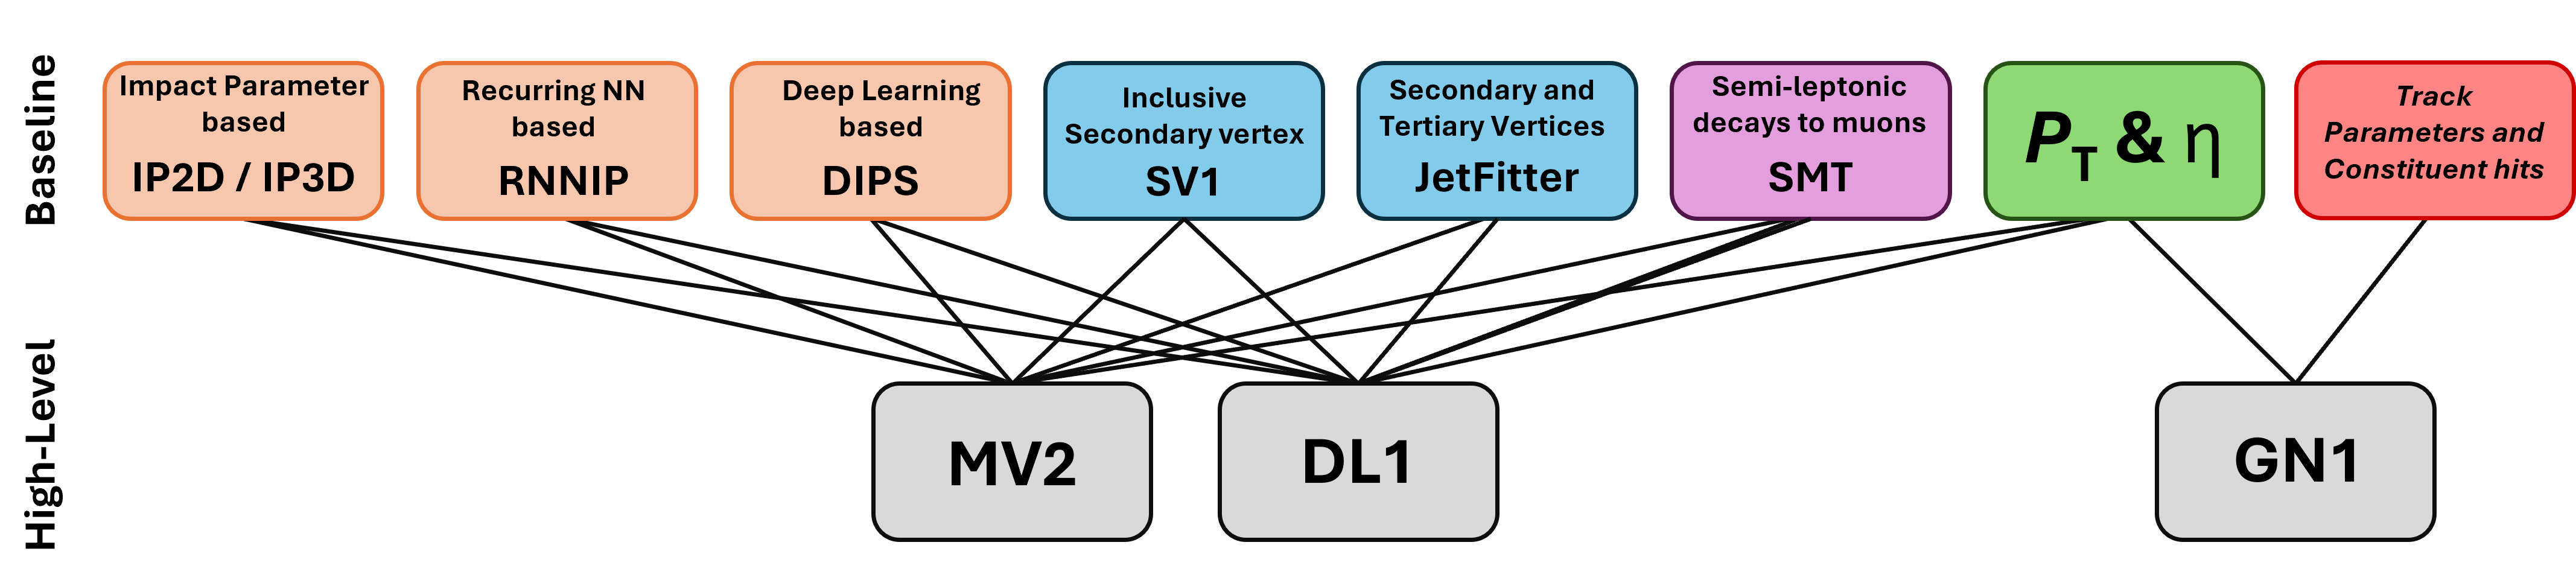
\includegraphics[scale=0.5]{figs/ch4/ftag-diagram.png}
    \caption{ Diagram of FTAG baseline and high-level taggers.}
\label{fig:ftag-diagram}
\end{figure}

\subsection{Impact Parameter Algorithms}\label{sec:ip-algo}

A b-hadron has the longest lifetime of any quarks which results in a long decay length and a displaced secondary vertex. The \gls{ip} is the point of closest approach of 
tracks from the b-hadron decay to the primary vertex. This parameter can be split into two parts, the $\textrm{d}_{\textrm{0}}$ as seen in Figure \ref{fig:bjet-cartoon}, and 
a longitudinal part $\textrm{\textit{z}}_{\textrm{0}} \textrm{sin}{\theta}$. A variable of the \gls{ip} is the signed lifetime significances $\textrm{s}_{\textrm{d}_{\textrm{0}}}$ 
= $\frac{\textrm{d}_{\textrm{0}}}{\sigma_{\textrm{d}_{\textrm{0}}}}$ and $\textrm{s}_{\textrm{\textit{z}}_{\textrm{0}}}$ = $ \frac{\textrm{\textit{z}}_{\textrm{0}} \textrm{sin}{\theta}}{\sigma_{\textrm{\textit{z}}_{\textrm{0}} \textrm{sin}{\theta}}}$.
are calculated corresponding to the \gls{ip} divided by its uncertainty, as shown in Figure \ref{fig:ip-sig}. The sign of this variable is assigned by extrapolating the track back to the 
primary vertex. This value is negative if the jet axis has to be extended backwards from the primary vertex to cross the track or its projection, otherwise it's positive. 
The \gls{ip} algorithms are used to satisfy certain criteria such as: $\textrm{\textit{}}_{\textrm{T}}^{\textrm{track}} >$ 1 GeV, the \gls{ip}s have to fulfill  $|\textrm{d}_{\textrm{0}}| < $ 
1 mm, and $|\textrm{\textit{z}}_{\textrm{0}} \textrm{sin}{\theta}| <$ 1.5 mm. Additional requirements are required for the number of hits in the silicon layers: $\textrm{N}_{\textrm{hits}}^{\textrm{Si}}
\geq$ 7 as well as an upper limit of silicon and pixel layer holes  $\textrm{N}_{\textrm{holes}}^{\textrm{Si}} \leq$ 2 and  $\textrm{N}_{\textrm{holes}}^{\textrm{pixel}} \leq$ 1.
The following sections briefly describes the IPxD baseline taggers and the \gls{dips} tagger. The \gls{rnnip} tagger will not be described as it is outside the scope of this thesis.
\begin{figure}[H]
    \centering
    \subfloat[\centering ]{{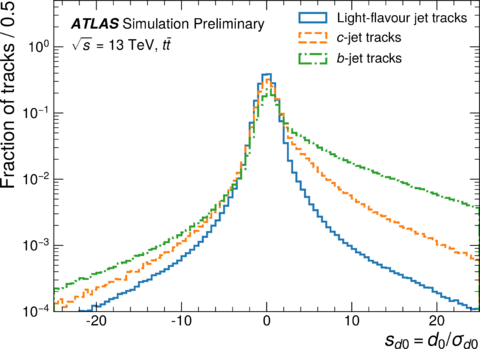
\includegraphics[scale=0.45]{figs/ch4/signed_d0.png}}}%
    \qquad
    \subfloat[\centering ]{{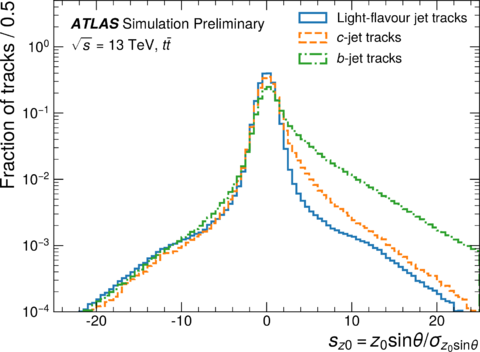
\includegraphics[scale=0.45]{figs/ch4/signed_z0.png}}}%
    \caption{ The signed IP significances variable shown for b-, c-, and light-jets for (a) transverse and (b) longitudinal components in $t\bar{t}$ events }
\label{fig:ip-sig}
\end{figure}

\subsubsection{IPxD}

The IPxD taggers comprise of two algorithms: the \gls{ip2d} which only uses the transverse \gls{ip} $\textrm{d}_{\textrm{0}}$ variable which tends to be less sensitive to pile-up, and 
the \gls{ip3d} tagger which uses both the transverse $\textrm{d}_{\textrm{0}}$ and $\textrm{\textit{z}}_{\textrm{0}} \textrm{sin}{\theta}$ variables \cite{btag-opt-2016}. The track categorization is based on 
pixel layer hit patterns as pre-defined by reference templates for b, c, and light hadrons. The final discriminant is a Log-Likelihood ratio (\gls{llr}) of probabilities of 
being any of the three hadrons. This \gls{llr} is described by Eq.~\ref{eq:4.7}.

\begin{equation}\label{eq:4.7}
    \textrm{IPxD}_{\textrm{l,c,cl}} = \sum_{\textrm{i}\in \textrm{tracks}} \textrm{log}\left(\frac{\textrm{P}^{\textrm{i}}_{\textrm{b,b,c}}}{\textrm{P}^{\textrm{i}}_{\textrm{l,c,l}}}\right)
\tag{4.7}
\end{equation}

The probability density functions to calculate $\textrm{P}_{\textrm{b}}$, $\textrm{P}_{\textrm{c}}$ and $\textrm{P}_{\textrm{l}}$ are extracted from \gls{mc} simulations.
Table \ref{tab:ipxd-variables} shows the six different variables for the IPxD tagger used to tag jets. The IPxD baseline taggers are used as input into the high-level taggers such as 
MV2 and DL1.

\begin{table}[t]
    \centering 
    \begin{tabular}{ |m{4em} |m{6cm} |}
        \hline
        \multicolumn{2}{|c |}{IPxD Discriminating Variables}\\
        \hline\hline
        Variable & Description \\
        \hline
         & LLR based on signed significance \\
         $\textrm{IPxD}_{\textrm{l}}$ & b- from light flavor jets \\
         $\textrm{IPxD}_{\textrm{c}}$ & b- from c-jets \\
         $\textrm{IPxD}_{\textrm{cl}}$ & c- from light flavor jets \\
         \hline
    \end{tabular}
    \caption{Variables for the IP2D and IP3D taggers (3 each)}
    \label{tab:ipxd-variables}
\end{table}

\subsubsection{DIPS}\label{sec:dips}

The \gls{dips} is a machine-learned algorithm that uses the \gls{ip} variables as input for a Deep Sets architecture \cite{Deep_sets}, treating the elements as a set without any specific order. 
The formalism of \gls{dips} has $\textit{\textrm{p}}_{\textit{\textrm{i}}}$ which is the vector representation of the inputs associated with the $\textit{\textrm{i}}^{\textit{\textrm{th}}}$ 
track in the jet, then the Deep Sets architecture applies its weight $\phi$ to each track. Tracks are then summed over and has additional processing in the form of a feed forward 
\gls{nn} (\textit{F}) as described in Eq. \ref{eq:4.8}.
%
\begin{equation}\label{eq:4.8}
    \mathcal{O}({\textit{\textrm{p}}_{\textrm{1}},...,\textit{\textrm{p}}_{\textit{\textrm{n}}}}) = \textrm{\textit{F}}\left(\sum^{\textrm{n}}_{\textit{\textrm{i}}=\textrm{1}}\phi (\textrm{\textit{p}}_{\textit{\textrm{i}}})\right)
\tag{4.8}
\end{equation}
%
where $\mathcal{O}({\textit{\textrm{p}}_{\textrm{1}},...,\textit{\textrm{p}}_{\textit{\textrm{n}}}})$ represents the b-, c-, and light- class probabilities. The architecture 
bisects the problem into operations over the inputs and over the sets. The track network $\phi$ extracts the relevant track information and the forwarding jet-network \textit{F} 
accounts for the correlations between the tracks \cite{DIPS}. Permutation invariance of the set is encoded using the sum operation. Since \gls{dips} encodes this permutation 
invariance, a much more natural representation of the data is made, allowing the machine learning (\gls{ml}) algorithm to be trained more effectively. This algorithm outperforms 
IPxD and \gls{rnnip} algorithms. 
\par
The \gls{ml} model of \gls{dips} outputs class probabilities of b-, c- and light-jets ($\textit{\textrm{p}}_{\textit{\textrm{b}}}, \textit{\textrm{p}}_{\textit{\textrm{c}}}, \textit{\textrm{p}}_{\textit{\textrm{l}}}$).
A discriminant is made from a combination of these three probabilities dictating whether a jet is b-tagged or not, this discriminant is given by Eq. \ref{eq:4.9}.
%
\begin{equation}\label{eq:4.9}
    \textit{\textrm{D}}_{\textit{\textrm{b}}} = \textrm{log} \frac{\textit{\textrm{p}}_{\textit{\textrm{b}}}}{(\textrm{1}-\textit{\textrm{f}}_{\textit{\textrm{c}}})\textit{\textrm{p}}_{\textit{\textrm{l}}}+\textit{\textrm{f}}_{\textit{\textrm{c}}}\textit{\textrm{p}}_{\textit{\textrm{c}}}}
\tag{4.9}
\end{equation}
%
where $\textit{\textrm{f}}_{\textit{\textrm{c}}}$ is a free parameter that helps balance the rejection rate between light-jets and c-jets for a given b-tagging efficiency. This 
is optimized post-training. A few input variables for \gls{dips} are scaled and shifted due to a mean that is not close to zero, this process is described in reference \cite{DIPS}. 
A list of \gls{dips} input features can be seen in Table \ref{tab:dips-variables}. The features that required additional preprocessing are noted.

\begin{table}[ht]
    \centering 
    \begin{tabular}{ |m{8em} |m{10cm} |m{5em} |}
        \hline
        \multicolumn{3}{|c |}{DIPS Input Features}\\
        \hline\hline
        Input & Description & Preprocessed\\
        \hline
         $\textrm{s}_{\textrm{d}_{\textrm{0}}}$ & $\textrm{d}_{\textrm{0}}$/$\sigma_{\textrm{d0}}$: Transverse IP significance &  \\
         $\textrm{s}_{\textrm{z}_{\textrm{0}}}$ & $\textrm{\textit{z}}_{\textrm{0}}\textrm{sin}\theta$/$\sigma_{\textrm{\textit{z}}\textrm{0sin}\theta}$: Longitudinal IP significance & \\
         $\textrm{log}\textrm{\textit{p}}_{\textrm{T}}^{\textrm{frac}}$ & $\textrm{log}\textrm{\textit{p}}_{\textrm{T}}^{\textrm{frac}}$ /$\textrm{\textit{p}}_{\textrm{T}}^{\textrm{jet}}$: Logarithm of fraction of the jet $\textrm{\textit{p}}_{\textrm{T}}$ & \checkmark \\
          & carried by the track &  \\
         $\textrm{log}∆\textrm{R}$ & Logarithm of opening angle between the track & \checkmark \\
          & and the jet axis & \\
         IBL hits & Number of hits in the IBL: could be 0, 1, or 2& \\
         PIX1 hits & Number of hits in the next-to-innermost pixel layer: could be 0, 1. or 2& \\
         shared IBL hits & shared IBL hits & \\
         split IBL hits & Number of split hits in the IBL& \checkmark \\
         nPixHits & Combined number of hits in the pixel layers& \\
         shared pixel hits & Number of shared hits in the pixel layers & \\
         split pixel hits & Number of split hits in the pixel layers& \\
         nSCTHits & Combined number of hits in the SCT layers& \checkmark \\
         shared SCT hits & Number of shared hits in the SCT layers& \\
         \hline
    \end{tabular}
    \caption{Input variables for DIPS}
    \label{tab:dips-variables}
\end{table}



\subsection{Secondary Vertex Algorithm}

The secondary vertex \gls{sv1} algorithm reconstructs a single displaced vertex in a jet using tracks. Due to hardware constraints, sometimes the track resolution in the \gls{id}
is not always able to resolve the entire decay cascade of a hadron in every jet. Therefore the criteria of reconstruction is only a single vertex, which is a good approximation
for a b-jet. The first step matches all two-track vertices, rejecting vertices that are compatible with tracks associated with long-lived particles, photon conversions or hadronic 
interactions with detector material. The next step is combine each accepted two-tracks into secondary vertices while removing all rejected tracks. Important information can 
be extracted from \gls{sv1} such as the vertex mass, decay length and its significance, number of associated tracks as well as the $∆\textrm{R}$ between the jet and the 
secondary vertex. Table \ref{tab:sv1} shows an overview of the variables for \gls{sv1}.

\begin{table}[ht]
    \centering 
    \begin{tabular}{ |m{5em} |m{14cm} |}
        \hline
        \multicolumn{2}{|c |}{SV1 Variables}\\
        \hline\hline
        Variable & Description \\
        \hline
         $\textrm{N}^{\textrm{SV1}}_{\textrm{trkAtVtx}}$ & Number of tracks associated to the SV \\
         $\textrm{N}^{\textrm{SV1}}_{\textrm{2trkAtVtx}}$ & Number of reconstructed two-track vertices candidates within the jet \\
         $\textrm{m}^{\textrm{SV1}}_{\textrm{inv}}$ & Invariant mass of the SV calculated from the associated tracks\\
         $\textrm{f}^{\textrm{SV1}}_{\textrm{E}}$   & Energy fraction of the SV associated tracks with respect to all tracks of the jet\\
         $∆\textrm{R}(\textrm{jet, SV})$    & $∆\textrm{R}$ between the jet axis and the secondary vertex relative to the primary vertex\\
         $\textrm{L}^{\textrm{SV1}}_{\textrm{xy}}$  & Reconstructed SV transverse decay length \\
         $\textrm{L}^{\textrm{SV1}}_{\textrm{xyz}}$ & Reconstructed SV decay Length \\
         $\textrm{S}^{\textrm{SV1}}_{\textrm{xyz}}$ & Decay Length significance \\
         \hline
    \end{tabular}\hfill
    \caption{ Variable overview for the SV1 algorithm \cite{btag-opt-2016}}
    \label{tab:sv1}
\end{table}

\subsection{JetFitter}

The decay chain multi-vertex reconstruction algorithm, a.k.a. JetFitter, is the second displaced vertex finder algorithm behind \gls{sv1} \cite{btag-opt-2016}. This algorithm 
aims to reconstruct the decay cascade topology of weakly decaying b- and c- hadrons. It assumes the primary, secondary, and the tertiary vertices are aligned in one line in the 
direction of the hadron's trajectory. The goal of this assumption is to cope with the finite track resolution. After an initial track selection of removing tracks associated to 
the primary vertex using a Kalman Filter \cite{kalman}. The resulting variables of JetFitter are shown in Table \ref{tab:jf-btag}. 
\par
This algorithm allows for special variables for the c-hadron exploiting the fact that the JetFitter vertex would be close to the primary vertex. These are chosen to differentiate 
the topologies between the b- and c- hadron. C-hadrons have lower decay multiplicity than the b-hadron due to their lower mass, thus decay products carry a larger momentum 
percentage along with a larger rapidity with respect to the jet axis. These variables are shown in Table \ref{tab:jf-ctag}.

\begin{table}[ht]
    \centering 
    \begin{tabular}{ |m{6em} |m{12cm} |}
        \hline
        \multicolumn{2}{|c |}{JetFitter Variables}\\
        \hline\hline
        Variable & Description \\
        \hline
         $\textrm{m}^{\textrm{JF}}_{\textrm{inv}}$ & Invariant mass of tracks associated to one or more displaced vertices \\
         $\textrm{f}^{\textrm{JF}}_{\textrm{E}}$ & Charged jet energy fraction in the secondary vertex \\
         $\textrm{S}^{\textrm{JF}}_{\textrm{xyz}}$ & Decay length significance of the displaced vertex\\
         $\textrm{N}^{\textrm{JF}}_{\textrm{1-trk vertices}}$   & Number of 1-track displaced vertices\\
         $\textrm{N}^{\textrm{JF}}_{\leq \textrm{2-trk vertices}}$ & Number of vertices with more than one track\\
         $∆\textrm{R}^{\textrm{JF}} (\textrm{P}_{\textrm{jet}}, \textrm{P}_{\textrm{vtx}})$     & $∆\textrm{R}$  between jet axis and the vectorial sum of all track momenta\\
         $\textrm{N}^{\textrm{JF}}_{\textrm{trks}}$  & Number of tracks associated to SV \\
         $\textrm{N}^{\textrm{JF}}_{\textrm{vertices}}$ & Number of reconstructed vertices \\
         \hline
    \end{tabular}\hfill
    \caption{ Variable overview of JetFitter algorithm for b-tagging \cite{btag-opt-2016}}
    \label{tab:jf-btag}
\end{table}

\begin{table}[H]
    \centering 
    \begin{tabular}{ |m{7em} |m{10cm} |}
        \hline
        \multicolumn{2}{|c |}{JetFitter C-Hadron Variables}\\
        \hline\hline
        Variable & Description \\
        \hline
         $\textrm{L}^{\textrm{\textrm{JF}}}_{\textrm{xyz}}$ & Displacement of SV from the primary vertex \\
         $\textrm{L}^{\textrm{\textrm{JF}}}_{\textrm{xy}}$ &  Transverse displacement of SV from the primary vertex\\
         $\textrm{min}(\textrm{Y}^{\textrm{JF}}_{\textrm{trk}})$ & Minimal rapidity of tracks within the jet \\
         $\textrm{max}(\textrm{Y}^{\textrm{JF}}_{\textrm{trk}})$ & Maximum rapidity of tracks within the jet \\
         $\textrm{avg}(\textrm{Y}^{\textrm{JF}}_{\textrm{trk}})$ & Average rapidity of tracks within the jet\\
         $\textrm{min}(\textrm{Y}^{\textrm{JF}}_{\textrm{trk, SV}})$ & Minimal rapidity of SV tracks\\
         $\textrm{max}(\textrm{Y}^{\textrm{JF}}_{\textrm{trk, SV}})$ & Maximum rapidity of SV tracks\\
         $\textrm{avg}(\textrm{Y}^{\textrm{JF}}_{\textrm{trk, SV}})$ & Average rapidity of SV tracks\\
         $\textrm{m}^{\textrm{JF}}_{\textrm{inv}} $ & Invariant mass of tracks associated to the SV\\
         $∆\textrm{E}^{\textrm{JF}}$     & Energy of tracks associated to SV\\
         $\textrm{f}^{\textrm{JF}}_{\textrm{E}}$  & Charged jet energy fraction of SV \\
         $\textrm{N}^{\textrm{JF}}_{\textrm{trks}}$ & Number of tracks associated to the SV \\
         \hline
    \end{tabular}\hfill
    \caption{ Variable overview of JetFitter algorithm for c-tagging \cite{btag-opt-2016}}
    \label{tab:jf-ctag}
\end{table}

\section{High-Level Taggers}

Baseline taggers are optimized for single properties of b-hadron decays. High-level taggers are multivariate taggers comprised of the baseline taggers previously described 
and as seen in Figure \ref{fig:ftag-diagram}. There are three high-level taggers that are currently deployed in ATLAS: the boosted decision tree (\gls{bdt}) based tagger MV2, 
the deep learning based DL1 and the graph \gls{nn} GN1. Currently, DL1 is the standard tagger within \gls{atlas}, but GNN based taggers have proven to be more effective and are currently being developed to replace it. DL1 is 
explored in higher detail in chapter \ref{ch5}. 

\subsection{Working Points}

As briefly discussed in Section \ref{sec:muon-reco}, \gls{wp}s are deployed for the high-level taggers to cover various needs in physics analyses. These \gls{wp}s are defined using 
the b-tagging efficiency on $t\bar{t}$ \gls{mc} samples. These single cut \gls{wp}s are used since having a full continuous b-tagging discriminant would require a continuous 
calibration in extremely fine efficiency bins. This task would take enormous time and require immense complexity. The tagging efficiency is described in Eq. \ref{eq:4.10}
%
\begin{equation}\label{eq:4.10}
    \varepsilon^{\textrm{j}} = \frac{\textrm{N}^{\textrm{j}}_{\textrm{pass}}(\mathcal{D} > \textrm{T}_\textrm{f})}{\textrm{N}^{\textrm{j}}_{\textrm{total}}} 
\tag{4.10}
\end{equation}
%
where $\textrm{N}^{\textrm{j}}_{\textrm{pass}}(\mathcal{D} > \textrm{T}_\textrm{f})$ are the number of jets of flavor \textit{j} passed the cut $\textrm{T}_{\textrm{f}}$ on the tagger 
discriminant $\mathcal{D}$ and $\textrm{N}^{\textrm{j}}_{\textrm{total}}$ are all jets of flavor j before the cut. The \gls{wp}s are defined based on b-jet efficiency $\varepsilon^{\textrm{j}}$
evaluated on $t\bar{t}$ \gls{mc} samples. In \gls{atlas} there are four \gls{wp}s defined as seen in Table \ref{tab:bjet-eff}. The inverse of each \gls{wp} characterizes the c- and light- jet rejection rate.
Misidentification improves with lower signal efficiency, therefore rejecting more background, trading off lower signal statistics. Within a physics analysis, every jet that passes a 
\gls{wp} is considered a b-jet. Each high-level tagger that is described in the following sections have different rates of b-tagging efficiencies, meaning the number of tagged 
b-jets in an analysis will depend on which tagger is used. Therefore high tagging efficiencies are sought after, encouraging physicists to use the latest technological advances.
The \gls{bdt} based MV2 was the standard tagger until Deep Sets architectures overtook and shown to be much more efficient, thus DL1 has now become the new standard. 
Recent developments in the past year has shown that graph \gls{nn}s can exploit track information much more profoundly, resulting in much higher tagging efficiencies than 
the DL1 tagger and is expected to take its place.

\begin{table}[ht]
    \centering 
    \begin{tabular}{ |m{6em} |m{4cm} |}
        \hline
        \multicolumn{2}{|c |}{Working Points for B-Tagging in ATLAS}\\
        \hline\hline
        Cut & b-tagging efficiency \\
        \hline
        loose & 85\% \\
        medium & 77\% \\
        tight & 70\% \\
        very tight & 60\% \\
        \hline
    \end{tabular}\hfill
    \caption{ Summary of b-tagging single cut WPs}
    \label{tab:bjet-eff}
\end{table}


\subsection{MV2}

The high-level tagger MV2 used to be the recommended tagger for EMTopo jets for Run 2 of ATLAS. This tagger used 24 inputs from the baseline taggers as input for the \gls{bdt}
training as well as $\textrm{\textit{p}}_{\textrm{T}}$ and $|\textrm{η}|$. Training the MV2 tagger used what is called a \textit{hybrid} sample which is a mixture of $t\bar{t}$ and Z' 
events. This is to ensure there is a large coverage of the $\textrm{\textit{p}}_{\textrm{T}}$ spectrum. The \gls{bdt} used b-jets as the signal class and c- and light- jets as a background class.
To balance the performance between the c-jet and light-jet rejection, a c-jet fraction $\textrm{f}_{\textrm{c}}$ was set to 7\% and therefore a light jet fraction of 93\%. The end result 
was named MV2c10. Figure \ref{fig:mv2_eff} shows the performance of the MV2, DL1 and baseline taggers in terms of background rejection as a function of b-tagging efficiency.

\begin{figure}[H]
    \centering
    \subfloat[\centering ]{{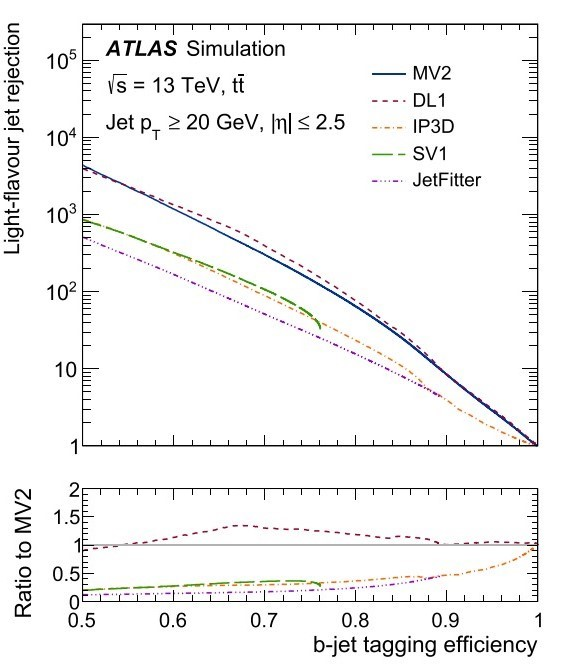
\includegraphics[scale=0.5]{figs/ch4/mv2_effu.jpg}}}%
    \qquad
    \subfloat[\centering ]{{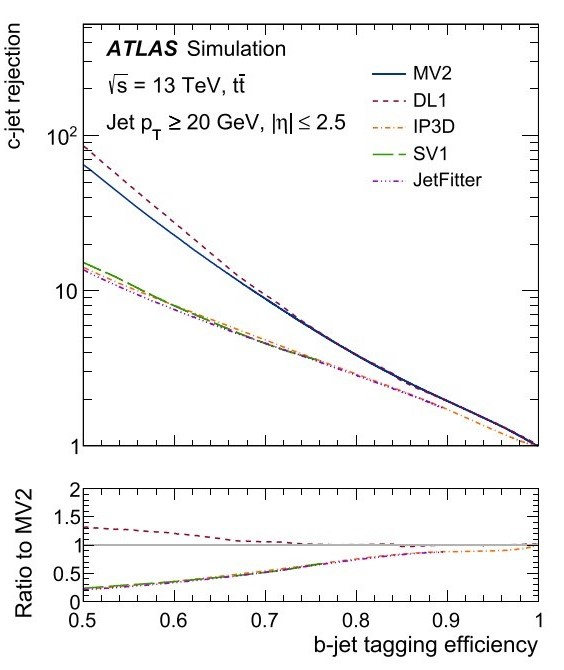
\includegraphics[scale=0.5]{figs/ch4/mv2_effb.jpg}}}%
    \caption{ The (a) light-jet and (b) c-jet rejections versus the b-jet tagging efficiency for the baseline taggers IP3D, SV1, JetFitter and the high level taggers MV2 and DL1. Evaluated on $t\bar{t}$ MC events \cite{btag-iden-eff}}
\label{fig:mv2_eff}
\end{figure}

\subsection{DL1}\label{sec:DL1-ch4}

The high-level DL1 tagger is a deep feed-forward \gls{nn} with three output nodes that correspond to the b-, c-, and light- flavor jet probabilities. The ReLU activation function is used 
for each layer while the last layer uses the softmax activation function. Using the softmax function for the output layer allows the output to be interpreted as probabilities. 
The final b-tagging log-likelihood discriminant score is calculated from the multi-class output using Eq. \ref{eq:4.11}.
%
\begin{equation}\label{eq:4.11}
    \mathcal{D}_{\textrm{b}}(\textrm{f}_{\textrm{c}}) = \textrm{log}\left(\frac{\textrm{p}_{\textrm{b}}}{\textrm{f}_{\textrm{c}} \cdot \textrm{p}_{\textrm{c}} + (\textrm{1}-\textrm{f}_{\textrm{c}}) \cdot \textrm{p}_{\textrm{l}} }\right)
\tag{4.11}
\end{equation}
%
where $\textrm{p}_{\textrm{b}}$, $\textrm{p}_{\textrm{c}}$ and $\textrm{p}_{\textrm{l}}$ are the output scores of DL1 representing the probabilities for the jet to be a b-jet, c-jet 
or a light-jet, respectively. The c-jet fraction $\textrm{f}_{\textrm{c}}$ allows tuning to balance the performance of the c-jet and light-jet rejection. The c-jet rejection increases 
as a function of $\textrm{f}_{\textrm{c}}$ and light-flavor decreases as a function of $\textrm{f}_{\textrm{c}}$. An advantage of using the DL1 compared to MV2 is that the 
discriminant can be rewritten to perform c-jet tagging with b-jet rejection. This new rewritten discriminant can be seen in Eq.~\ref{eq:4.12}
%
\begin{equation}\label{eq:4.12}
    \mathcal{D}_{\textrm{c}}(\textrm{f}_{\textrm{b}}) = \textrm{log}\left(\frac{\textrm{p}_{\textrm{c}}}{\textrm{f}_{\textrm{b}} \cdot \textrm{p}_{\textrm{b}} + (\textrm{1}-\textrm{f}_{\textrm{b}}) \cdot \textrm{p}_{\textrm{l}} }\right)
\tag{4.12}
\end{equation}
%
where  $\textrm{f}_{\textrm{b}}$ is a floating value for the b-jet fraction. DL1 has shown many positives over MV2. The tagger is effectively maintained with much less person power,
while also fewer variables have to be calculated and stored, saving computing power. The DL1 tagger is a family of high-level multivariate taggers. These taggers differ from the 
baseline tagger inputs, they are as follows: baseline DL1, DL1r, DL1rmu, and DL1d. The DL1 baseline uses the same variables as MV2 with the additional JetFitter variables for c-jet 
identification. DL1r configuration uses the \gls{rnnip} instead of the baseline IPxD taggers. The DL1rmu exploits the soft-muon information. Lastly, the DL1d uses the baseline taggers 
SV1, JetFitter but uses the \gls{dips} instead of the baseline IPxD. More information is given on the DL1d tagger in Chapter \ref{ch5}.


\subsection{GN1}\label{sec:gn1}

The GN1 tagger is currently the latest and greatest particle identification algorithm. It differs from the previously described high-level taggers in a few ways. GN1 does not make 
use of the underlying baseline taggers but instead exploits the internal structure of the jet through the use of two auxiliary training objectives: the grouping of tracks originating 
from a common vertex, and the prediction of the underlying physics processes \cite{gnn-ftag}. The graph neural network takes 2 kinematic and 21 track variables as training input. Using auxiliary 
tasks removes the need to add the baseline taggers, therefore simplifying the training process and allowing the tagger to be more versatile in training phase space. The algorithm 
is trained on \textit{truth-information} obtained through simulations. 
\par
The GN1 combines a graph neural network architecture with auxiliary training objectives. Initially, the two jet inputs (transverse momentum and signed pseudorapidity) are fed 
into a per-track initialization network with three hidden layers, each containing 64 neurons. These three layers are a Deep Sets architecture such as the technique used by DL1.
A fully connected graph is built from the outputs of these three Deep Set layers. Each node $\textrm{\textit{h}}_{\textrm{i}}$ in the graph represents a single track in the jet, 
characterizing a feature vector. The output nodes from the Deep Set architecture are used to populate the graph. Outputs from each graph layer are aggregated features of each node 
$\textrm{\textit{h}}_{\textrm{i}}$ and neighboring nodes $\textrm{\textit{N}}_{\textrm{i}}$. The feature vectors of each node are fed into a fully connected \gls{nn} layer that 
produces updated values of the vector. These updated features are used to compute edge scores of each node (scores calculated from neighboring nodes). A non-linear activation 
function is used while a softmax function calculates weights for each pair of nodes using the edge scores. Finally, an updated node representation is computed by taking the 
weighted sum over each updated node representation. After the graph network is implemented, these outputs are used in a node classification network to predict track truth origin. 
A diagram of the entire network architecture is seen in Figure \ref{fig:gnn-diagram}. The track and jet kinematic input variables for the \gls{gn1} tagger are listed in Table~\ref{tab:gn1-var} within the Appendix \ref{appendix:gn1-upgrade}. The next version of \gls{gn1} is called GN2 and is currently expected to replace its predecessor. 

\begin{figure}[h]
    \centering
    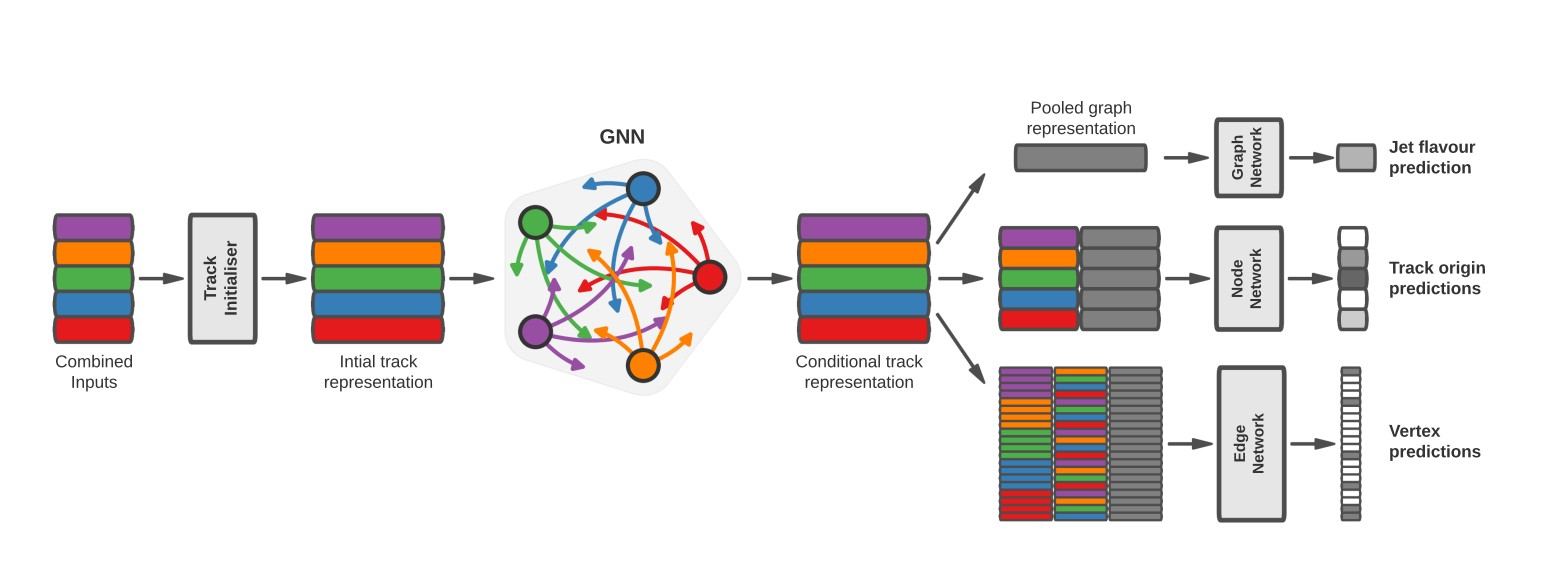
\includegraphics[scale=0.38]{figs/ch4/GNN-diagram.jpg}
    \caption{ The network diagram of GN1. First, a Deep Sets architecture is used to populate node features in a GNN. The GNN outputs are used to predict jet flavor, track origins, and track-pair vertex compatibility. \cite{gnn-ftag}}
\label{fig:gnn-diagram}
\end{figure}



\section{Event Simulation}\label{sec:event-sim}

Simulated \gls{pp} events are used in every physics analysis while also being vital in event reconstruction calibrations. They also play an important role in simulating \gls{bsm} 
models which are used to help define new phases spaces for the chance of detecting new physics. Simulated events are used later in this thesis as \gls{ml} input and are vital 
in deploying efficient particle identification algorithms. \gls{bsm} simulations are also used in the Anomaly Detection analysis in Chapter~\ref{ch6} to show separation 
between standard \gls{sm} events and the anomalous \gls{bsm} events. 
\par
Event simulations not only simulate kinematics of particles within the \gls{sm} (or beyond of it) but are also used to show how simulated particles would interact with the 
\gls{atlas} detector. Due to the complexity of integral emerging from \gls{qft} calculations, Monte Carlo \gls{mc} techniques are used in the simulations \cite{workman}.

\subsection{Monte Carlo Generators}


Every event generation is typically divided into two parts: the matrix element generation that describes the hard scatter and secondly the parton showering and hadronization modeling 
which includes the initial state radiation (\gls{isr}) and the final state radiation (\gls{fsr}). The matrix element and the parton shower can be calculated mostly perturbatively, other 
calculations cannot. There are several common mathematical models used to simulate hadronization: the Lund string model and the cluster model. In the Lund string model, the connection 
between a quark and an antiquark is modeled as a string, assuming the potential between the two to be linearly increasing with distance. These strings then split according to a 
Fragmentation function forming a new quark-antiquark pair. This process continues until only stable hadrons remain \cite{Lund-string}. The cluster model is based on \gls{qcd} confinement where 
neighboring partons build color clusters which then decay into two hadrons who also will decay until stable hadrons are formed \cite{Jan-cluster}. Figure \ref{fig:mc-diagram} shows a simplified \gls{mc} simulation.
\par
The steps of calculated the matrix elements, parton showers, hadronization and the underlying soft radiation can all be simulated by the common generators \texttt{PYTHIA8} \cite{pythia-stefan}, \texttt{HERWIG7} \cite{herwig},
\texttt{SHERPA} \cite{sherpa-enrico}, \texttt{POWHEGBOX} \cite{powheg}, and \texttt{MADGRAPH5\_@aMCNLO} \cite{madgraph}. A few drawbacks to some of these generators are: \texttt{PYTHIA8} provides mainly leading order calculations which are typically not sufficient since next-to-leading 
order (\gls{nlo}) corrections would have to be applied and these can be fairly large. \texttt{HERWIG7} is only used for parton showering even though it does include \gls{nlo}s, the fraction 
of negative event weights can be very large. The generators of \texttt{POWHEGBOX} and \texttt{MADGRAPH5\_@aMCNLO} are used to provide higher order calculations while also being able to 
be interfaced into \texttt{PYTHIA8} and \texttt{HERWIG7} to calculate the parton showering. To describe models that use non-perturbative processes, parameters must be tuned using 
collision data. The most common used parameters in \gls{atlas} are the A14 \cite{pythia-para} parameters for \texttt{PYTHIA8} or the H7UE \cite{herwig-para} parameters for \texttt{HERWIG7}.

\subsection{Detector Simulation}

The last step of simulation is to simulate the \gls{atlas} detector. \gls{mc} generators don't take into account the detector, the final state output needs to be translated to a 
signal that represents the detector's output. A full \gls{atlas} detector simulation is done in two parts. The first step is to incorporate the detector geometry, this is done 
by a program called \texttt{GEANT4} \cite{geant4}, this provides highly precise modeling of particle interactions with each sub-detector. This process is so precise that it takes a large 
fraction of computing power that \gls{atlas} uses. Therefore techniques have been developed to decrease this computational power by mimicking the output of \texttt{GEANT4} in the 
use of fast simulator algorithms \cite{fastsim}. These algorithms use thousands of individual parametrizations of calorimeter response. This process uses a lot less computational resources with 
a trade-off of precision. These fast simulations are widely used by \gls{atlas}.

\begin{figure}[H]
    \centering
    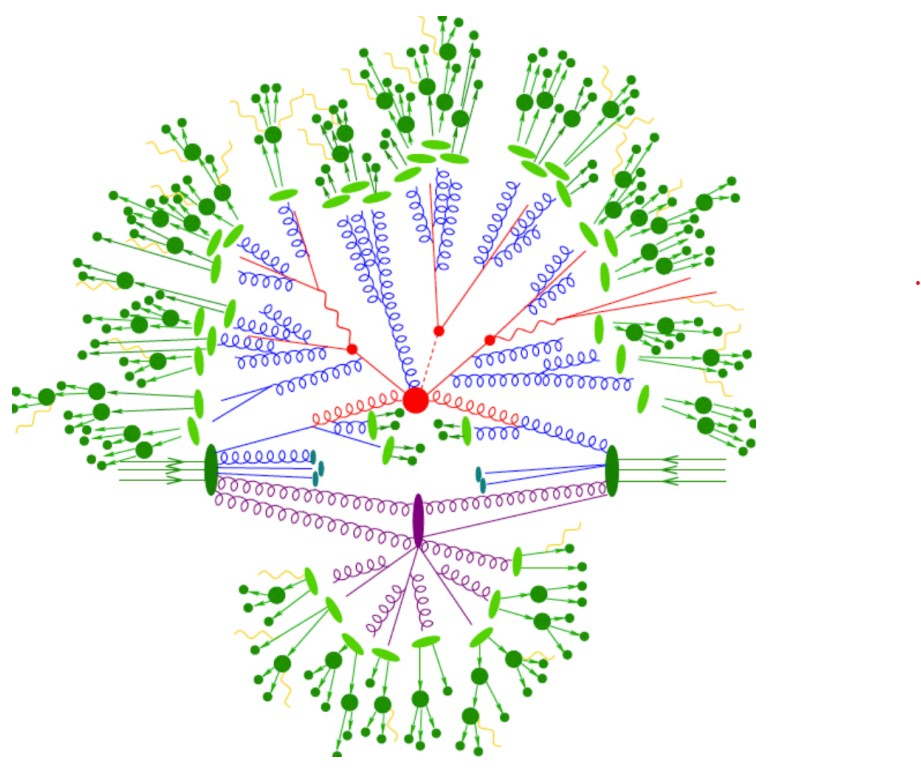
\includegraphics[scale=0.65]{figs/ch4/mc-diagram.jpg}
    \caption{ Illustration of a hadron-hadron collision simulated by a MC generator. The center red circle signifies the hard scatter collision while the purple oval represents underlying soft-scatter events. The red and blue tree-like structures depict QCD bremsstrahlung simulated by parton showering. The other elements are hadronization (light green), hadron decays (dark green), and photon radiation (yellow). \cite{parton-showering}}
\label{fig:mc-diagram}
\end{figure}

\begingroup
\clearpage% Manually insert \clearpage
\let\clearpage\relax% Remove \clearpage functionality
\vspace*{-16pt}% Insert needed vertical retraction
\chapter[DEEP LEARNING MODEL TRAINING FOR THE HL-LHC]{DEEP LEARNING MODEL TRAINING FOR THE HL-LHC}
\label{ch5}
\endgroup

The high-level tagger \gls{dl1} was introduced during Run 2 of the \gls{atlas} detector as the second high-level tagger beside \gls{mv2} and originally used \textit{EMPTopo} jets. 
The tagger was designed to combine the base-line taggers as discussed in \ref{sec:heavyFlavorTagging} into a final discriminant score as seen in Eq. \ref{eq:5.1}. Introducing 
the human-designed detector level base-line taggers into a machine learned algorithm brought several benefits such its multi-class output of the probabilities for each 
flavor of jet (b-jet, c-jet and light-jet). Creating a \gls{nn} brings flexibility and customization which is why they are preferred over \gls{bdt}s.
\par
This next chapter discusses the training of the \gls{dl1} tagger using the \gls{dips} base-line tagger, creating the DL1d high-level tagger. This model was trained using simulations 
of the \gls{atlas} detector with its new geometry after its upgrade to transition into Run 4. Implementing the \gls{itk} detector as discussed in Chapter 3, Section \ref{sec:hllhc-itk}.
These simulations include the increased pile-up from the \gls{hllhc} of $\langle \upmu \rangle$ = $\textrm{200}$. The jet structure used are the \textit{PFlow} discussed in 
Section \ref{sec:small-R}. 

\section{DL1 Design}

The underlying structure the the \gls{dl1} tagger is a deep feed-forward \gls{nn} with three output nodes corresponding to b-, c-, and light-flavor probabilities as seen in Figure \ref{fig:dl1-arch}.
The \gls{relu} activation function is used for each hidden layer while the output layer utilizes the softmax activation 
function to ensure the output can be interpreted as probabilities. These multi-class outputs are then used to calculate a final discriminant score as seen in the 
reintroduced \gls{dl1} discriminant log-likelihood function \ref{eq:5.1}.
%
\begin{equation}\label{eq:5.1}
    \mathcal{D}_{\textrm{b}}(\textrm{f}_{\textrm{c}}) = \textrm{log}\left(\frac{\textrm{p}_{\textrm{b}}}{\textrm{f}_{\textrm{c}} \cdot \textrm{p}_{\textrm{c}} + (\textrm{1}-\textrm{f}_{\textrm{c}}) \cdot \textrm{p}_{\textrm{l}} }\right)
\tag{5.1}
\end{equation}
%
Here $\textrm{p}_{\textrm{b}}$, $\textrm{p}_{\textrm{c}}$, and $\textrm{p}_{\textrm{l}}$ are the multi-class probability outputs for b-, c-, and light-flavor jets. The $\textrm{f}_{\textrm{c}}$
is an introduced c-jet fraction tunable parameter which can give emphasis to the c-jet or light-jet rejection performance. This parameter is expected to be tuned for each tagger 
as its value depends on the needs of the physics analyses. As previously discussed, this fraction can gives rise to the ability to flip the \gls{dl1} tagger to focus on b-jet and 
light-jet rejection, requiring the reintroduced log-likelihood discriminant equation \ref{eq:5.2}.  
%
\begin{equation}\label{eq:5.2}
    \mathcal{D}_{\textrm{c}}(\textrm{f}_{\textrm{b}}) = \textrm{log}\left(\frac{\textrm{p}_{\textrm{c}}}{\textrm{f}_{\textrm{b}} \cdot \textrm{p}_{\textrm{b}} + (\textrm{1}-\textrm{f}_{\textrm{b}}) \cdot \textrm{p}_{\textrm{l}} }\right)
\tag{5.2}
\end{equation}
%
Here there are the same multi-class probability scores as seen in \ref{eq:5.1} but the tunable parameter has now changed to a b-jet fraction, $\textrm{f}_{\textrm{b}}$. Due to its 
ease of training and maintainability, the \gls{dl1} tagger requires less man-power and creates reliable tagging scores that reduce the amount of necessary stored information, saving 
on memory. 
%
\begin{figure}[h]
    \centering
    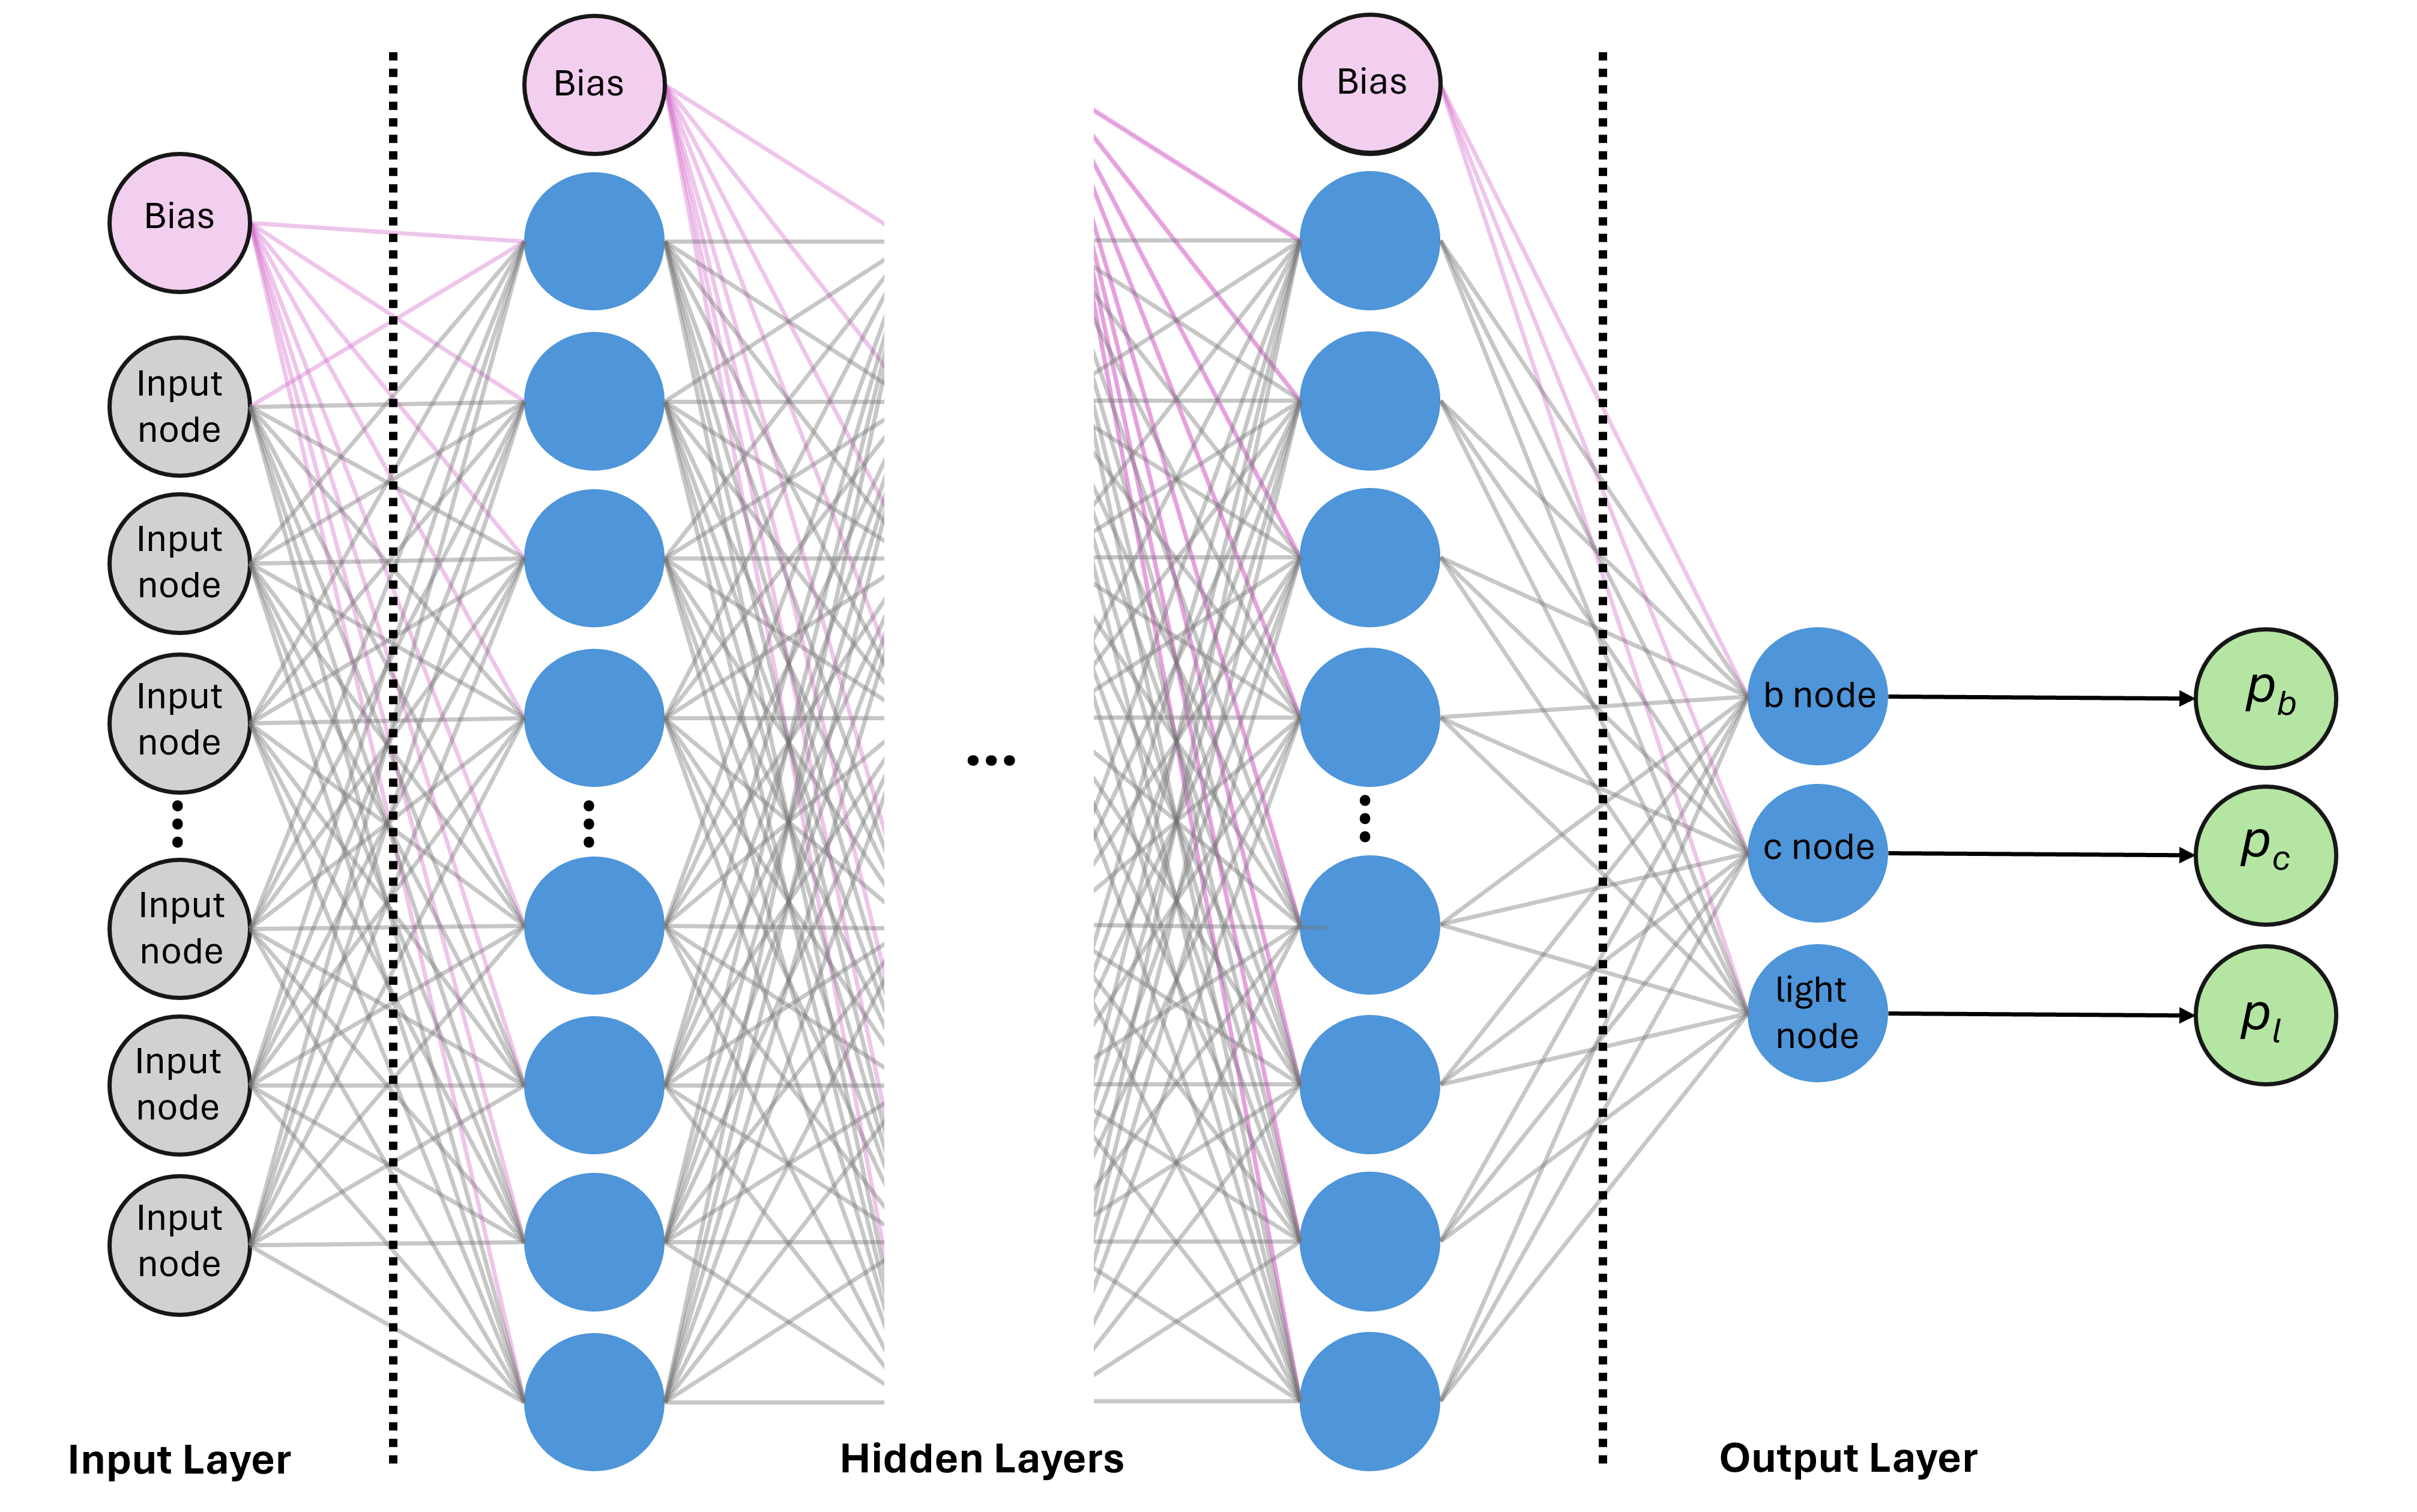
\includegraphics[scale=0.5]{figs/ch5/DL1-arch.png}
    \caption{ Deep feed-forward architecture of DL1 with unspecified number of nodes}
\label{fig:dl1-arch}
\end{figure}
%
As discussed previously, the \gls{dl1} family contains four different types of taggers that utilize different baseline information. The first is the baseline \textit{DL1} that 
uses the same input baseline tagger variables as MV2 (as seen in \ref{tab:ipxd-variables}, \ref{tab:sv1},\ref{tab:jf-btag}) with the additional JetFitter variables for c-tagging 
as seen in table \ref{tab:jf-ctag}. From there the baseline \textit{DL1} is used with additional \gls{nn} inputs. \textit{DL1r} uses the baseline \textit{DL1} with additional 
flavor probabilities from the \gls{rnnip} algorithm. \textit{DL1rmu} exploits the soft-muon information from the muon spectrometer while also including the inputs from the 
\textit{DL1r}. Lastly, the latest tagger is the \textit{DL1d} which is the baseline \textit{dl1} that includes an additional feed-forward \gls{nn} called \gls{dips} that was 
previously discussed in Section \ref{sec:dips}. A diagram of the \gls{dl1} family is seen in Figure \ref{fig:dl1-fam}.

\begin{figure}[h]
    \centering
    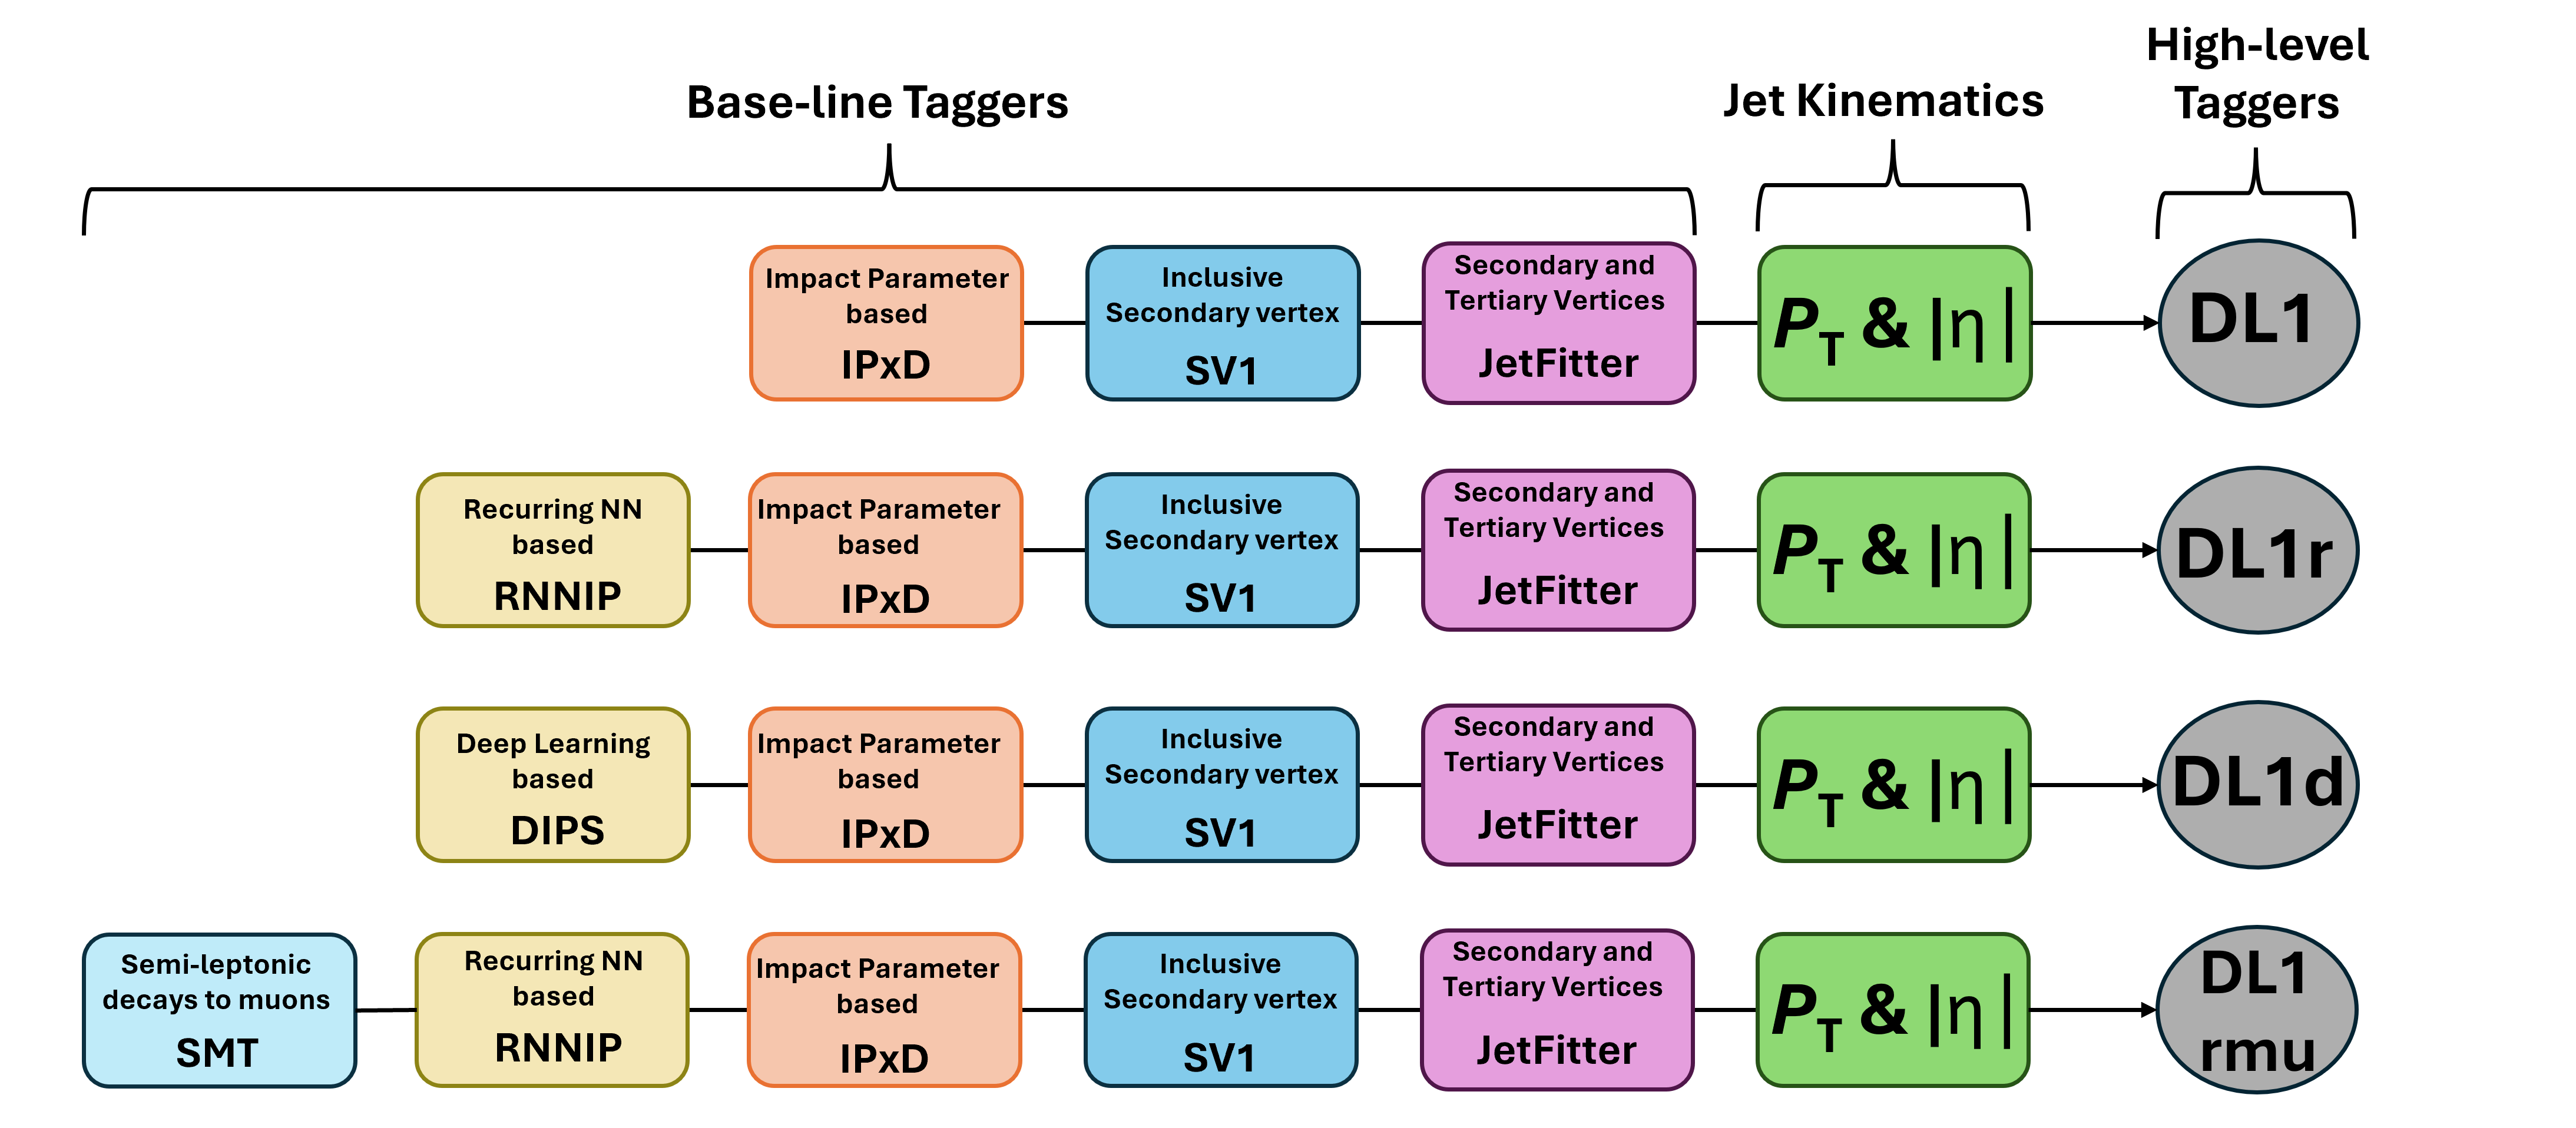
\includegraphics[scale=0.5]{figs/ch5/dl1_fam.png}
    \caption{ Structures of the DL1 tagger family, differing in NN input variables }
\label{fig:dl1-fam}
\end{figure}

\subsection{DL1d design}

In the following sections, training of the DL1d model for the \gls{hllhc} is described. Since the DL1d utilizes the deep learning model \gls{dips}, its design if fairly more complex than the 
other DL1 models in the family. The architecture design can be seen in Figure \ref{fig:dl1d-design}. Notice there are two sub-networks $\upphi$ and \texttt{F} which correspond to the \gls{dips} architecture. The 
\gls{dips} model is trained using track variables described in Table \ref{tab:dips-variables}. Each track in a jet is first processed through the network $\upphi$. In the next step, all \texttt{n}
track networks, corresponding to the number of tracks in a jet, are summed up and further processed via the network \texttt{F}. This can be summarized via an equation as seen:
%
\begin{equation}\label{eq:5.3}
    \overrightarrow{\textrm{P}}_{\textrm{i}} = \texttt{F}\left(\sum_{i=1}^{n}\upphi({\overrightarrow{x}_{\textrm{i}}^{\textrm{t}}})\right)
\tag{5.3}
\end{equation}
%
where $\overrightarrow{x}_{\textrm{i}}^{\textrm{t}}$ are the track input features and $\overrightarrow{\textrm{P}_{\textrm{i}}}$ is the vector of the b-, c-, and light flavor jet class probabilities
corresponding to the \gls{dips} output.

\begin{figure}[h]
    \centering
    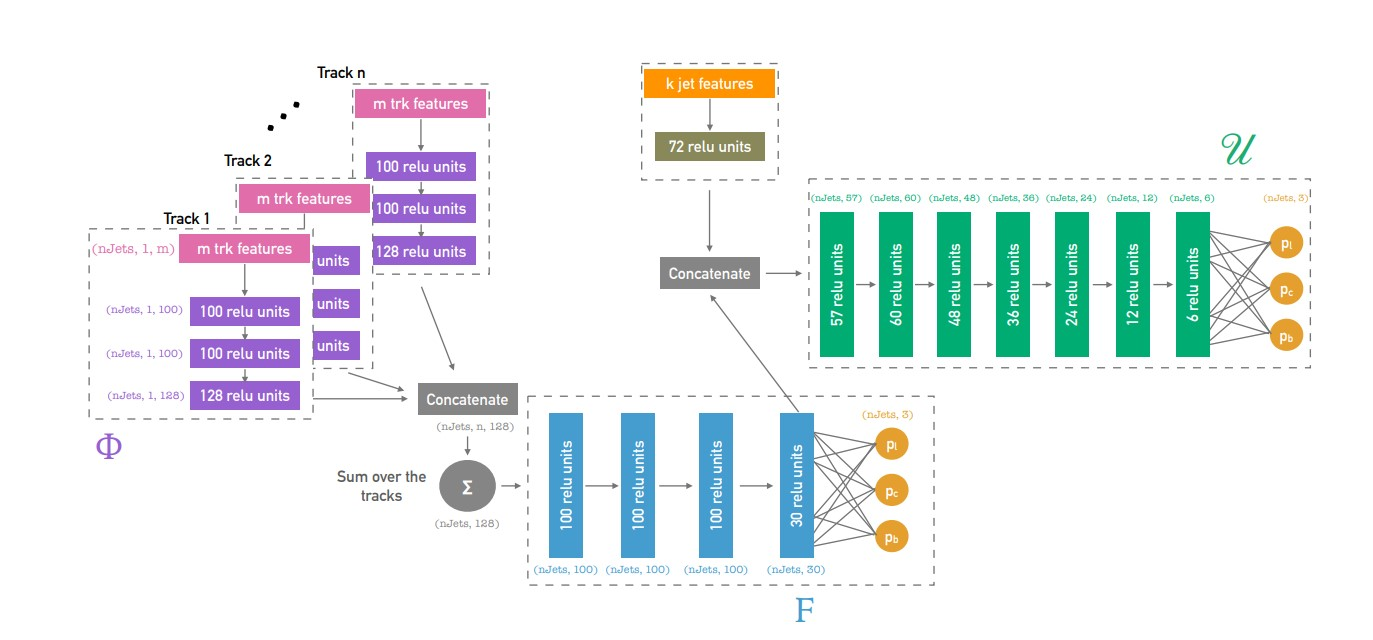
\includegraphics[scale=0.5]{figs/ch5/dl1d-design.jpg}
    \caption{ Architecture of DL1d combining the DIPS $\upphi$ and \texttt{F} networks to the DL1 feed-forward nodes \textit{$\mathscr{U}$} }
\label{fig:dl1d-design}
\end{figure}

The \gls{dips} networks,$\upphi$ and \texttt{F}, are joined to the DL1d feed-forward architecture denoted as \textit{$\mathscr{U}$}. A joint architecture allows the passing of more information into the \gls{dl1} 
\gls{nn} \textit{$\mathscr{U}$}. In the case of Figure \ref{fig:dl1d-arch}, a layer of 30 nodes is concatenated with the other jet features that are processed through a network containing 72 nodes. 
A full back-propagation up to all the track \gls{nn}s $\upphi$ is done during the training allowing a joint optimization of all three networks. The \gls{dips} networks have intermediate losses 
which are used to determine the performance and optimization of the \gls{dips} model prior to being used as input to the \gls{dl1} network. The final feed-forward \gls{dl1} architecture \textit{$\mathscr{U}$}
has three output nodes to calculate the multi-class probabilities. Both networks have dedicated losses. While the loss of the final \textit{$\mathscr{U}$} network \textit{L}($\mathscr{U}$) is sensitive 
to track features and jet kinematics, the loss of \textit{F} network \textit{L}(\textit{F}) is only sensitive to tracks. The overall optimization is performed over the combined loss, as shown:

\begin{equation}\label{eq:5.4}
    \textrm{\textit{L}}(\textrm{comb.}) = \textrm{\textit{L}}(\textit{$\mathscr{U}$}) + \lambda \cdot \textrm{\textit{L}}(\textrm{\textit{F}})
\tag{5.4}
\end{equation}


\section{Software Chain}

The software chain from training the \gls{dl1} tagger to validation and deployment in the \gls{atlas} software \texttt{ATHENA} are unassociated. The training of the \gls{nn} 
is based on the industry-standard open-sourced coding language Python3.6~\cite{python}. The packages numpy~\cite{numpy} and pandas~\cite{pandas} are used for data handling
while it's formatted in the HDF5 format~\cite{hdf5}. The \gls{atlas} software package developed to convert root datasets into HDF5 format is called the Training Dataset Dumper (\gls{tdd})
The code structure is configured using human-readable formats such as JSON~\cite{json} and yaml to ensure user compatibility.
For the \gls{nn} training, Tensorflow~\cite{tensorflow} is used with a Keras2~\cite{keras} frontend. These packages are used to create a user-friendly framework for deep learning training 
called Umami which handles the preprocessing and training steps. For visualization, the package matplotlib~\cite{matplotlib}  and tools from 
scikit-learn~\cite{scikit} are included in the training scripts. These tools are compiled into a convenient tool in the Umami family named Puma. The full workflow (Umami and Puma) can be 
performed using a Docker image~\cite{docker} which allows the software to be ran 
from any computer without the need to install the necessary environment. The output model is then transformed into a format called LightWeight Tagger Neural Network~\cite{lwtnn} (\gls{lwtnn})
which integrates the model into the \gls{atlas} software \texttt{ATHENA}.

\section{Preprocessing}

The first step before training a \gls{dl1} model is preparing the input in a step called \textit{preprocessing}. To ensure robustness of a model to perform properly over a large 
$\textrm{\textit{p}}_{\textrm{T}}$ spectrum, two simulated samples are combined into a \textit{hybrid sample}. One sample is of $t\bar{t}$ events and the other is of a \gls{bsm} particle 
called $\textrm{Z}'$. An example $\textrm{\textit{p}}_{\textrm{T}}$ spectrum of these two samples can be seen in Figure \ref{fig:hybrid-noscale} in (a). The $\textrm{Z}'$ allows a flat $\textrm{\textit{p}}_{\textrm{T}}$ spectrum of up to 4.5 TeV with a 
total range up to 6 TeV. This $\textrm{Z}'$ sample is known as an \textit{extended $\textrm{Z}'$} sample since the normal distribution of a $\textrm{Z}'$ is up to about $\approx$4 TeV. The $t\bar{t}$ sample populates the lower $\textrm{\textit{p}}_{\textrm{T}}$ spectrum, ensuring there are enough statistics for a proper model to be trained while the $\textrm{Z}'$ populates 
larger $\textrm{\textit{p}}_{\textrm{T}}$ to increase tagging efficiencies for heavier particles. This sample, along with all that is included in this thesis, are using PFlow objects. 
The object selection within the $t\bar{t}$ sample is of the following:
%
\[
 t\bar{t} \ \textrm{selection :} \begin{cases}
       \textrm{b-jets} & \textrm{b-hadron} \ \textrm{\textit{}}_{\textrm{T}} < \textrm{250 GeV}\\ 
       \textrm{c-jets} & \textrm{jet} \ \textrm{\textit{p}}_{\textrm{T}} < \textrm{250 GeV}\\
       \textrm{light-jets} & \textrm{jet} \ \textrm{\textit{p}}_{\textrm{T}} < \textrm{250 GeV}\\
\end{cases}\]
%
As noted here, the b-jet selection uses b-hadron $\textrm{\textit{p}}_{\textrm{T}}$. The sample fraction of $t\bar{t}$ and $\textrm{Z}'$ can be adjusted, in the following example plots, 
the fraction is adjusted to 70\% $t\bar{t}$ and 30\% $\textrm{Z}'$. The merged \textit{hybrid sample} can be seen in (b) of Figure \ref{fig:hybrid-noscale}.

\begin{figure}[h]
    \centering
    \subfloat[\centering ]{{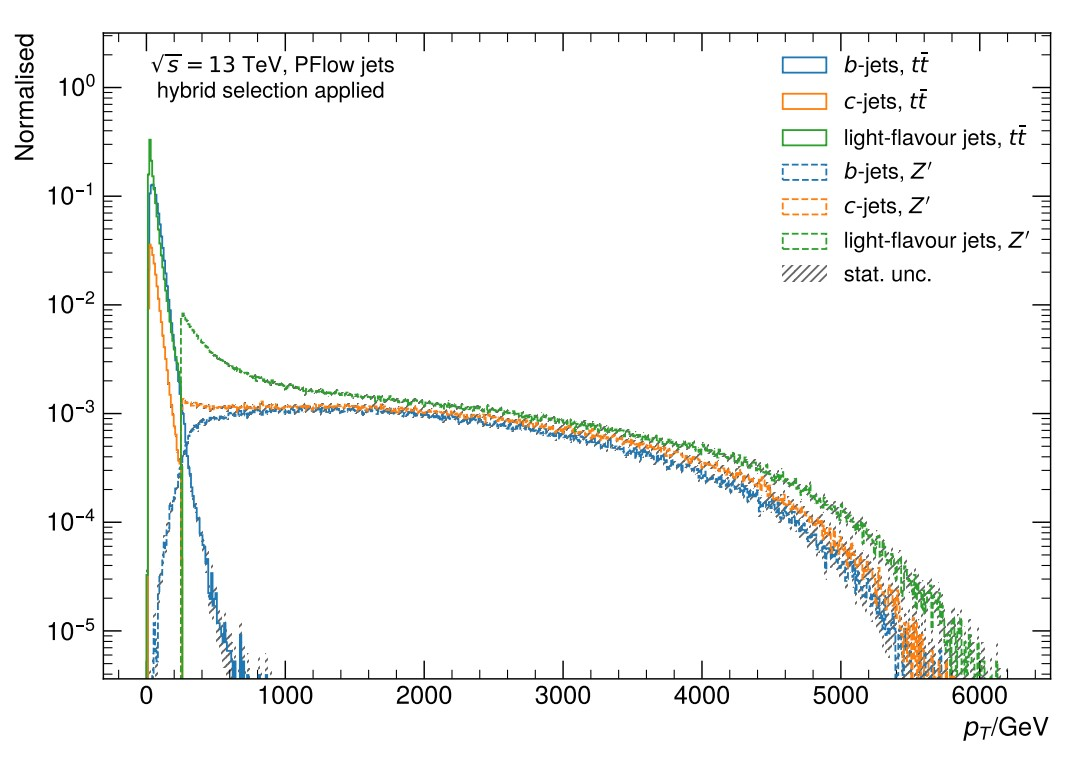
\includegraphics[scale=0.29]{figs/ch5/nohybrid_noscale.jpg}}}%
    \subfloat[\centering ]{{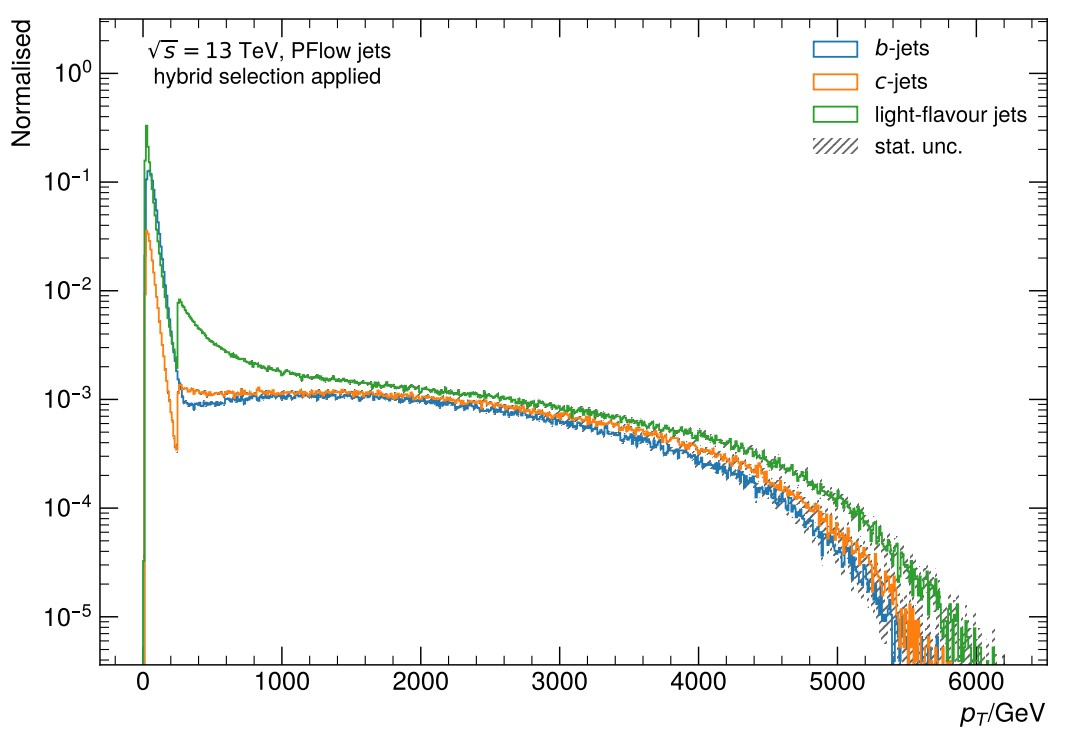
\includegraphics[scale=0.29]{figs/ch5/hybrid_noscale.jpg}}}%
    \caption{  (a) $\textrm{\textit{p}}_{\textrm{T}}$ distribution of $t\bar{t}$ sample (solid lines) and a Z$'$ sample (dashed lines). The $t\bar{t}$ b-jet distribution is normalized to unity and all other distributions are normalized to the b-jet distribution. (b) Samples from (a) merged into one distribution normalized to b-jet distribution }
\label{fig:hybrid-noscale}
\end{figure}

The goal of the \gls{dl1} tagger is to differentiate between hadron flavors. As seen in Figure \ref{fig:sample_fractions}, the flavor composition is imbalanced towards light-flavor 
jets. In order to avoid kinematic and count biases within the tagger, a resampling step must be applied. This also helps mitigate discontinuity between the two 
combined samples. Kinematic correlations are important for the baseline taggers, the goal for the high-level tagger is to avoid differences in kinematics and attempt to tag hadrons 
by jet-by-jet classification. Instead of weighting each sample fraction to match a chosen distribution, a resampling method is deployed to avoid instabilities in the model training 
steps. There are two methods of resampling. There is \textit{undersampling} where single jets are removed from the majority classes to fit a distribution of a minority class or 
there is \textit{oversampling} where jets from minority classes are duplicated to match a given distribution. Figure \ref{fig:resampling_diagram} shows a diagram of both methods. A combined method called 
Importance Sampling with Replacement, also referred to as \textit{PDF} sampling, undersamples and oversamples distributions to match a middle target distribution while enforcing the 
same shape. As seen in Figure \ref{fig:sample_fractions}, b-jets are a middle distribution, therefore the PDF sampling is used in the preprocessing step of the following work.

\begin{figure}[h]
    \centering
    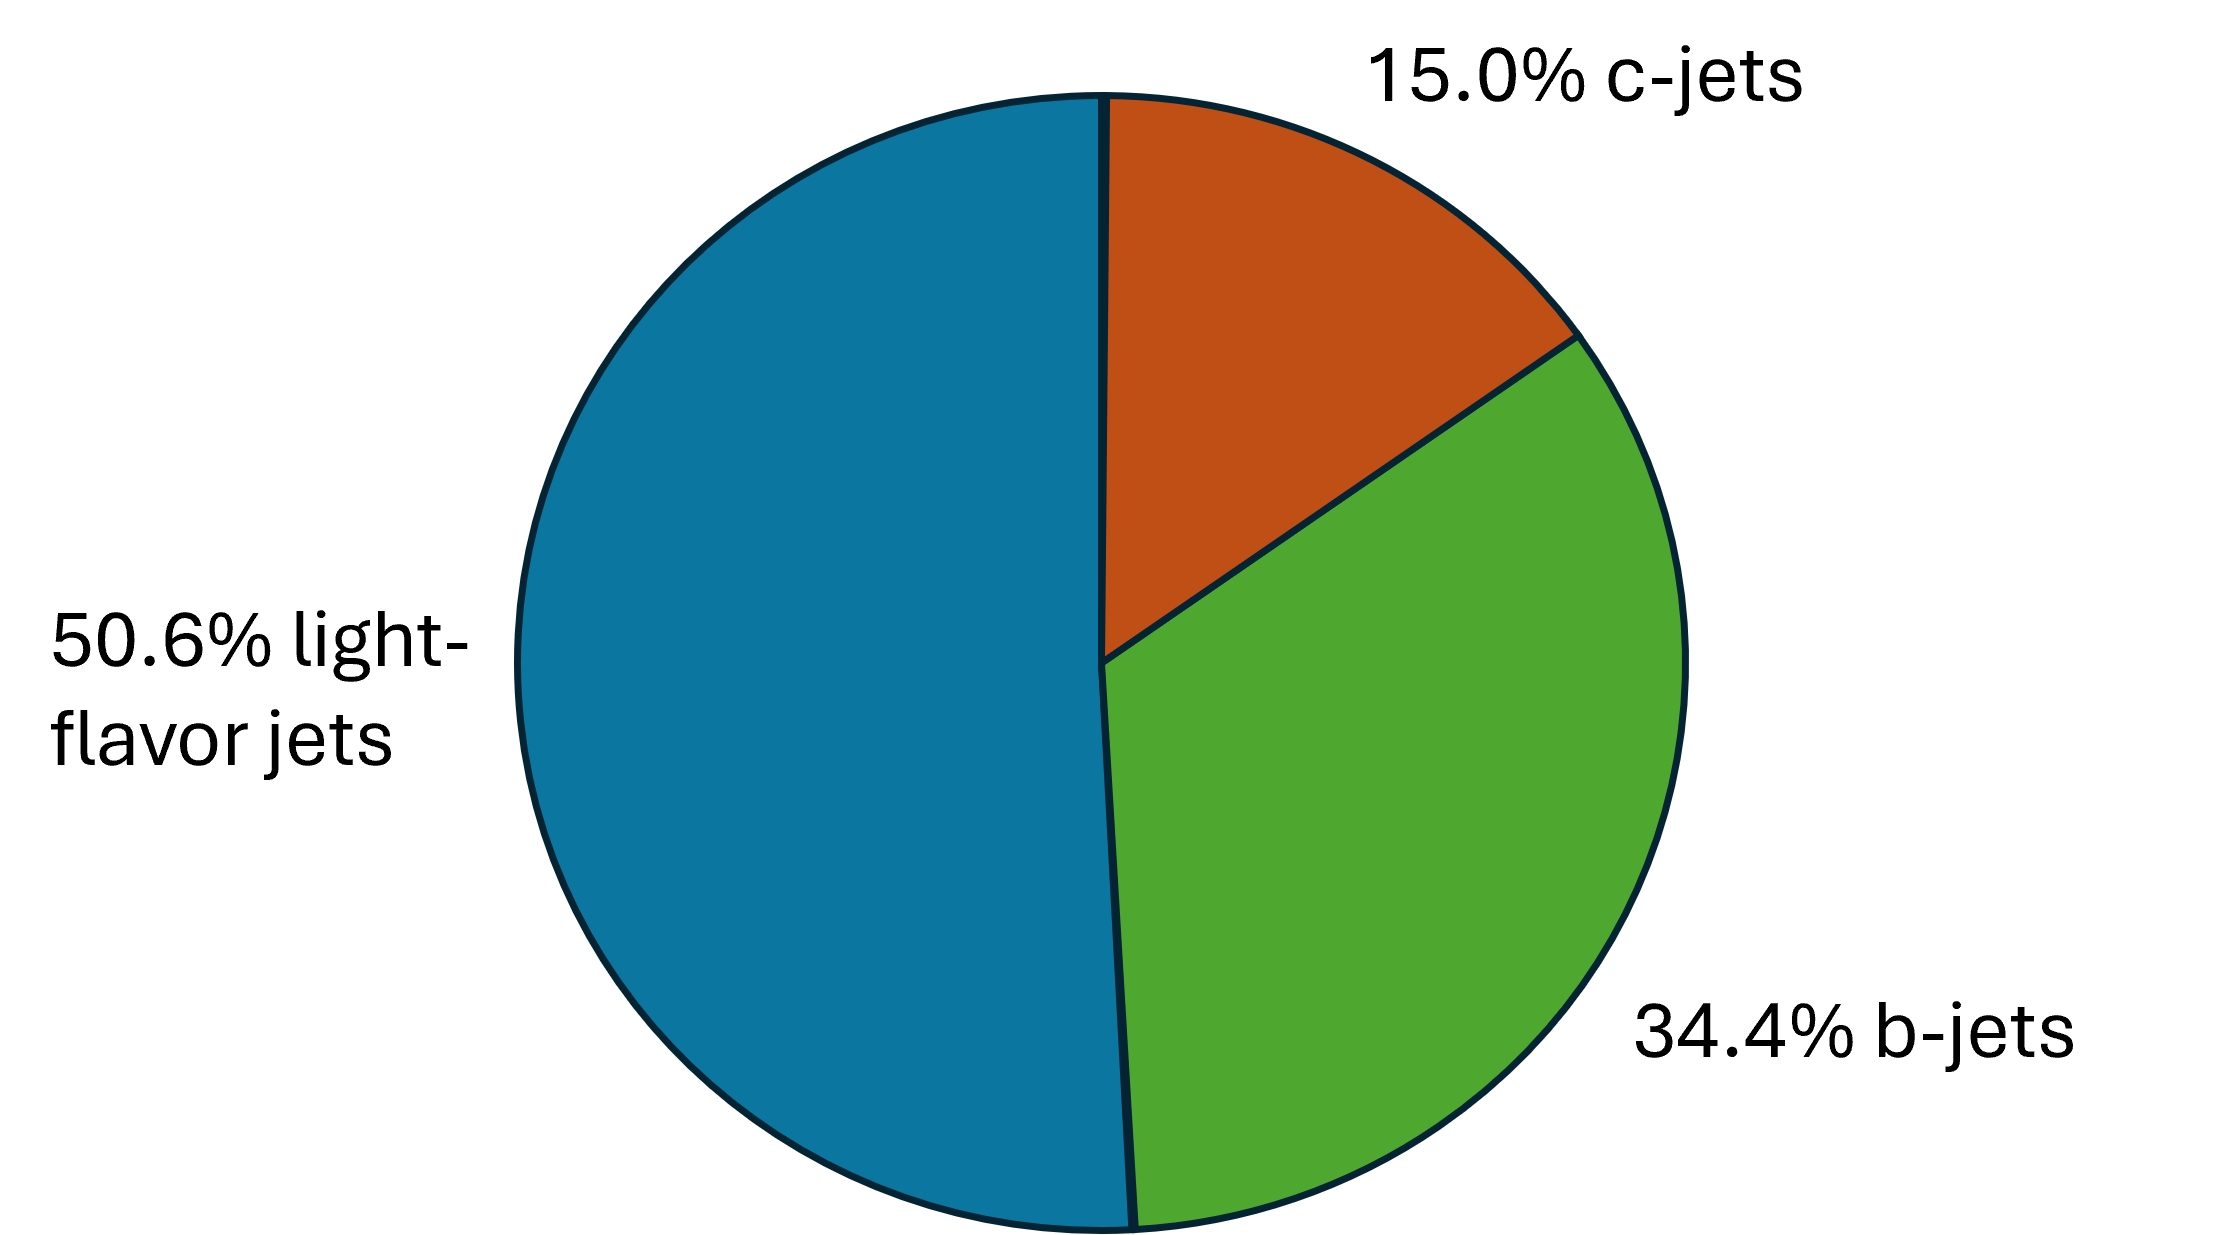
\includegraphics[scale=0.6]{figs/ch5/ex_comp_pie.png}
    \caption{ Hybrid sample hadron fractions.}
\label{fig:sample_fractions}
\end{figure}

\begin{figure}[h]
    \centering
    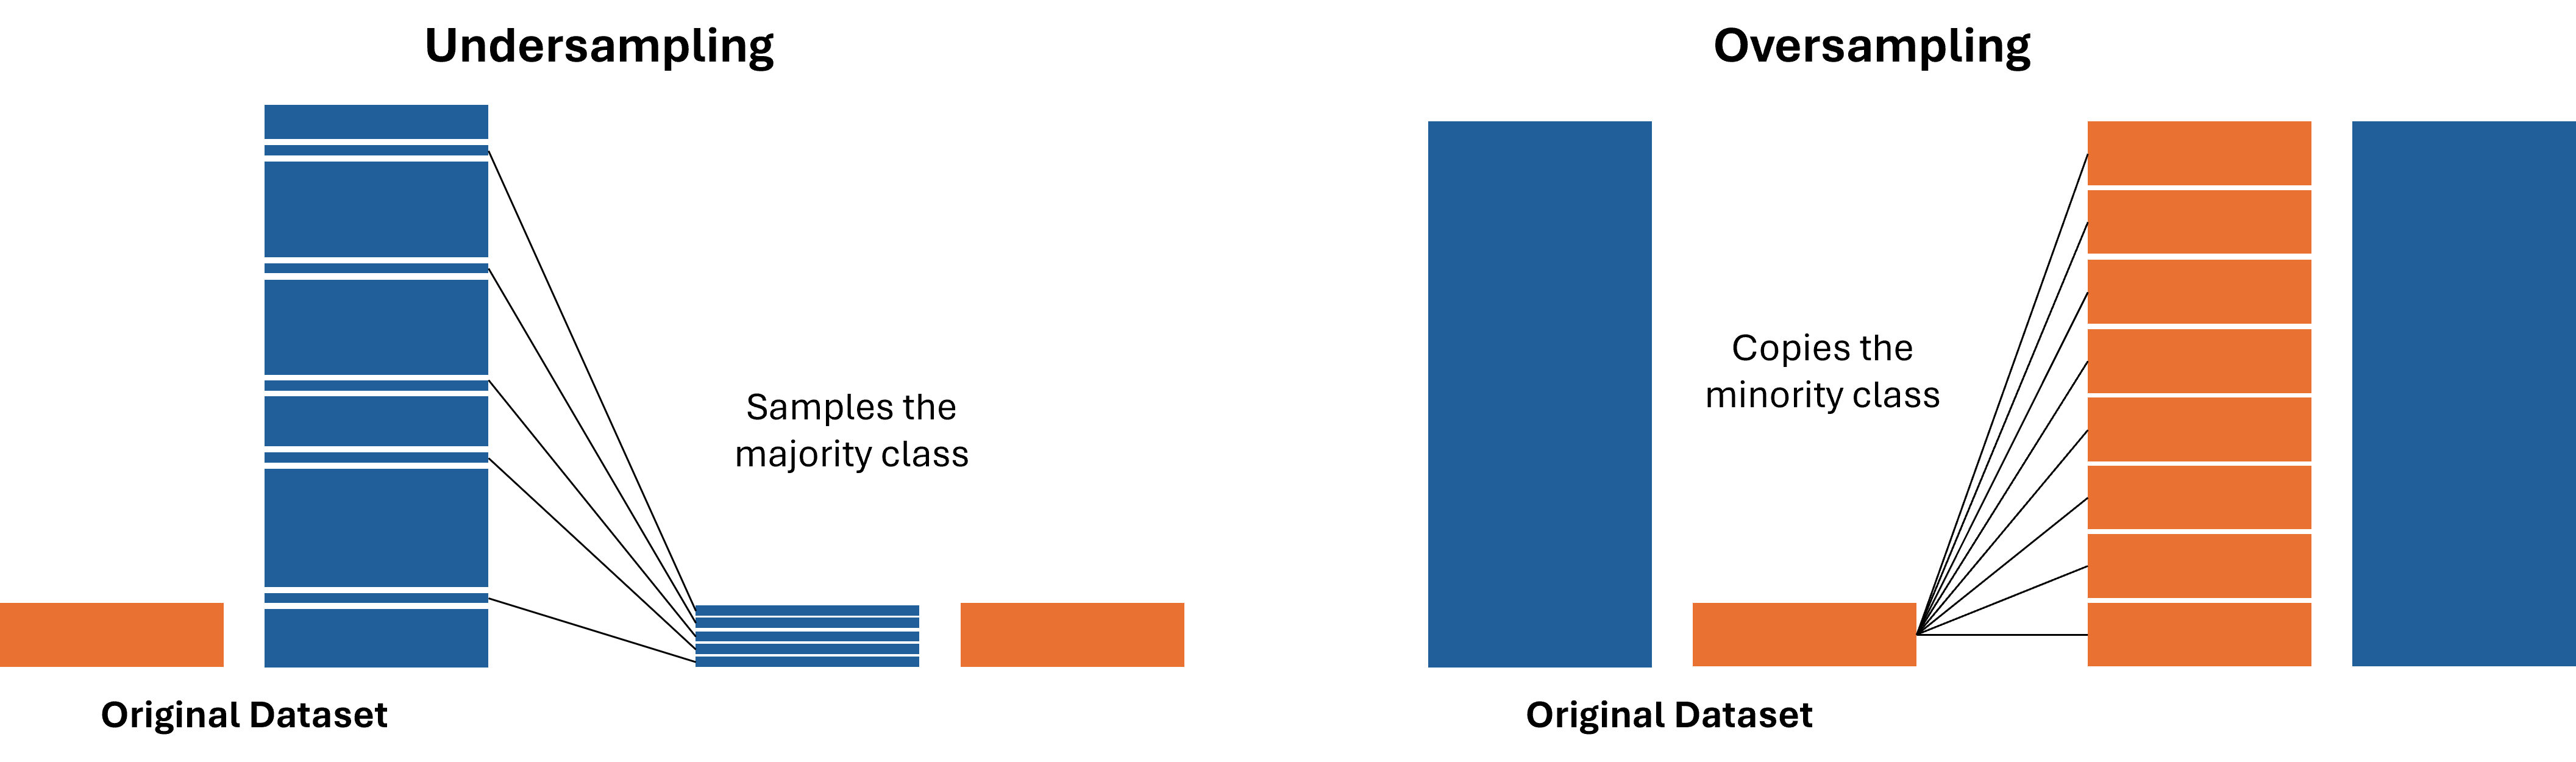
\includegraphics[scale=0.5]{figs/ch5/Sampling-diagram.png}
    \caption{ Diagram of the resampling methods to ensure balanced model training.}
\label{fig:resampling_diagram}
\end{figure}

The obvious issue that is present in these sampling methods is the duplication of events during oversampling a minority distribution. This may cause 
a bias due to the lack of diversity of statistics in the minority groups. Luckily, the samples are \gls{mc} produced and therefore the statistics can be
simply increased by producing more samples through event generators. However, a resampling procedure referred to as the \textit{count method} was studied as a comparison
to the PDF method. The count method strictly only undersamples to the lowest distribution, thus drastically decreasing statistics in favor of bias possibilities. 
The $\textrm{\textit{p}}_{\textrm{T}}$ and $|\textrm{η}|$ b-jet distributions are taken as 
reference and the c-jet and light-jet flavor are resampled to match them. The binning used for the undersampling procedure tends to be more granular, especially 
in the lower $\textrm{\textit{p}}_{\textrm{T}}$ region where the sample transition bins are, while at higher $\textrm{\textit{p}}_{\textrm{T}}$ the bins are wider. This can 
be seen by resampling the example distribution from Figure \ref{fig:hybrid-noscale} in Figure \ref{fig:hybrid-scaled}.

\begin{figure}[h]
    \centering
    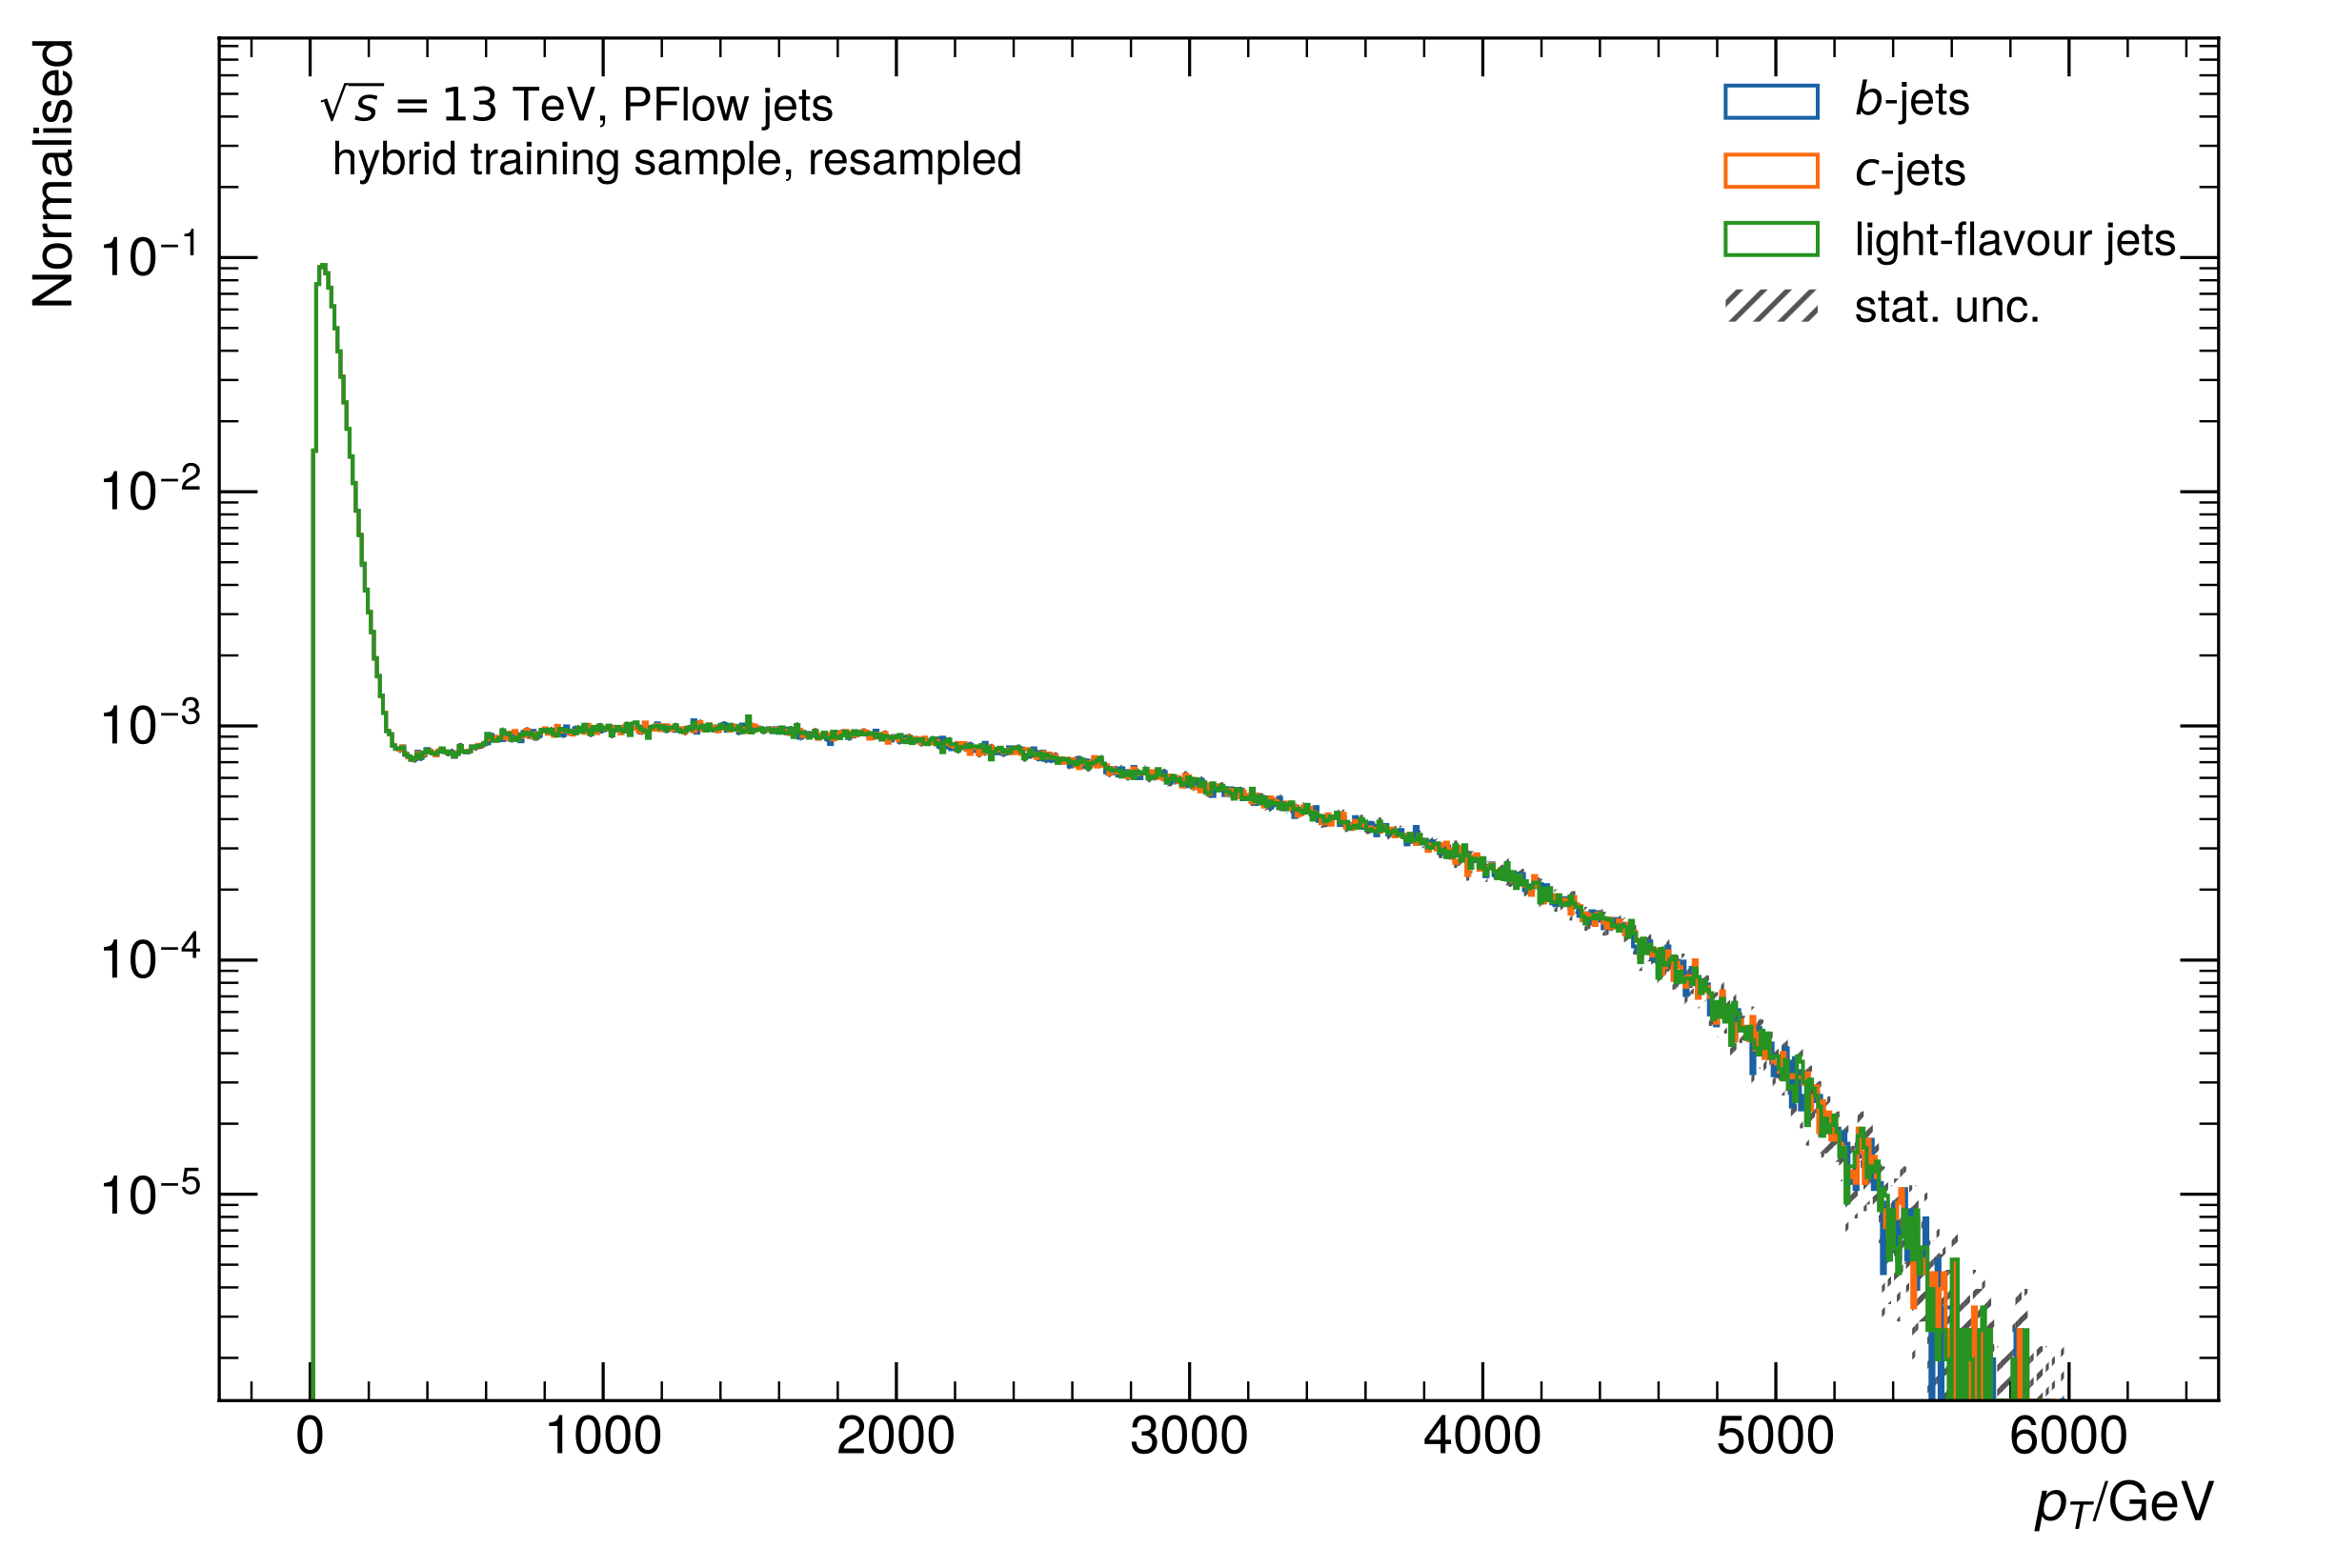
\includegraphics[scale=0.35]{figs/ch5/hybrid-scaled.png}
    \caption{ Resampled example flavor distributions.}
\label{fig:hybrid-scaled}
\end{figure}

Lastly before training, the ranges of the input variables need to be balanced so that they're all in the same order of magnitude, otherwise certain 
variables would carry more weight in the model training procedure. Therefore, all the variables are shifted to a mean of zero and a standard deviation 
of one, with the exception of binary check variables. Also, extremely anomalous events originating from obscure phase spaces within the samples are 
removed to secure an undisturbed training process.

\section{ HL-LHC Samples}

The current versions of these heavy-flavor taggers have been trained using simulated samples from Run 2. The latest versions that are being implemented as of 2023 have been 
optimized for Run 3 and are trained on the latest Run 3 samples. In the scope of this thesis, preliminary trainings for the DL1 tagger have been conducted using samples 
simulated using the \gls{itk} from Run 4 that starts in 2029 in order to see how well the new geometry can increase tagging efficiency with the main focus on the increase 
of $|\textrm{η}| \le$ 4. All objects simulated in these samples are PFlow objects as discussed in Section \ref{sec:small-R}.

\subsection{Object Selections}

The most important features for training effective taggers are tracks, therefore it's vital to simulate tracks through the new \gls{itk} detector with precision. These tracks represent 
trajectories of charged particles reconstructed from hits in the \gls{itk} pixels and strip sensors. The η-dependent variables underwent a combination of selections based on general track quality criteria and requirements 
specific to flavor tagging algorithms. The variables used in the baseline taggers (found in tables \ref{tab:ipxd-variables}, \ref{tab:sv1}, \ref{tab:jf-btag}) have adjusted criteria due to the 
pseudorapidity extension of the \gls{itk} detector. Only jets with $\textrm{\textit{p}}_{\textrm{T}} >$ 20 GeV and $|\textrm{η}| \le$ 4 are considered. A generator-level overlap removal with electrons 
and muons from W boson decays are also applied. Pile-up jet rejection algorithms are still under development for the \gls{hllhc}, so the selected jets are required to be matched within $∆\textrm{R} >$
0.3 with truth-jets built from hard-scatter stable particles that are clustered with the anti-$\textrm{\textit{k}}_{\textrm{T}}$ algorithm with R=0.4. The selected reconstructed primary vertex is required to be within 1 mm 
of the hard scatter vertex. Tracks are associated to jets using $\textrm{\textit{p}}_{\textrm{T}}$-dependent matching criteria, with a cone size of $∆\textrm{R} \approx$ 0.45 for jets with $\textrm{\textit{p}}_{\textrm{T}}$
= 20 GeV to $∆\textrm{R} \approx$ 0.25 for jets with $\textrm{\textit{p}}_{\textrm{T}} >$ 200 Gev. In cases where multiple tracks pass the criteria, the closest track is chosen. Jet flavor labels are assigned 
based on generator-level presence of b- or c-hadrons, or $\tau$ hadronic decays. If a b-hadron with $\textrm{\textit{p}}_{\textrm{T}} >$ 5 GeV is found within $∆\textrm{R}$ = 0.3, the jet is labeled a b-jet. 
This procedure is repeated for c-hadrons and $\tau$ hadronic decay products. Jets that have no labels by the end of this iteration are assumed to originate from light-flavor quarks and 
are labeled light-jets. Table \ref{tab:itk-req} shows the new requirements imposed on the jets due to the implementation of the \gls{itk} detector.

\begin{table}[ht]
    \centering 
    \begin{tabular}{ |c | c | c| c |}
        \hline
        \multicolumn{4}{|c |}{New Flavor Tagging Requirements for ITk}\\
        \hline\hline
        Requirements & \multicolumn{3}{|c|}{Pseudorapidity interval} \\ \cline{2-4}
                     & $|\textrm{η}|<$ 2 & 2.0 $< |\textrm{η}|<$ 2.6 & 2.6 $<|\textrm{η}|<$ 4.0 \\ 
        \hline
        pixel + strip hits & $\geq$ 9 &  $\geq$ 8 & $\geq$ 7 \\
        pixel hits & $\geq$ 1 & $\geq$ 1 & $\geq$ 1 \\
        pixel + strip holes & $\leq$ 2 & $\leq$ 2 & $\leq$ 2 \\
        $\textrm{\textit{p}}_{\textrm{T}}$ [MeV] & $>$ 900 & $>$ 500 & $>$ 500 \\
        $|\textit{\textrm{d}}_{\textrm{0}}|$ [mm] & $\leq$ 2.0 & $\leq$ 2.0 & $\leq$ 3.5 \\
        $|\textit{\textrm{z}}_{\textrm{0}}\textrm{sin}\theta|$ [mm] & $\leq$ 5.0 & $\leq$ 5.0 & $\leq$ 5.0 \\
        \hline
    \end{tabular}
    \caption{Training samples used for DL1d for HL-LHC studies \cite{run4-ftag}}
    \label{tab:itk-req}
\end{table}


\subsection{Sample Preprocessing}


The following samples consist of the necessary $t\bar{t}$ and $\textrm{Z}'$ samples for training with a \gls{cme} of 14 TeV which aligns with the predicted \gls{hllhc} beam energy. A small
sample of only 100,000 events is also used that include thes \gls{hgtd} (briefly discussed in Section \ref{sec:hgtd}) detector within the simulation step and is used for a few studies that are 
mentioned later in this chapter. These three samples are listed in table \ref{tab:dl1-samples}.


\begin{table}[ht]
    \centering 
    \begin{tabular}{ |c | c | c| c |c |}
        \hline
        \multicolumn{5}{|c |}{HL-LHC DL1 Training Samples}\\
        \hline\hline
        Sample & \multicolumn{0}{c}{Container} & & $\langle \upmu \rangle$ & \# of Events\\
        \hline
        $t\bar{t}$    & \multicolumn{1}{l}{mc15\_14TeV.600012.PhPy8EG\_A14\_ttbar\_hdamp258p75} & & 200 & 4,374,000\\
         & \multicolumn{0}{l}{\_nonallhad.recon.AOD.e8185\_s3654\_s3657\_r12573} & &  &   \\
        $\textrm{Z}'$ & \multicolumn{1}{l}{mc15\_14TeV.800030.Py8EG\_A14NNPDF23LO\_flatpT} & &   200 & 1,605,205 \\
         & \multicolumn{0}{l}{\_Zprime\_Extended.recon.AOD.e8185\_s3654\_s3657\_r12574}  & & & \\
         HGTD & \multicolumn{1}{l}{mc15\_14TeV.600012.PhPy8EG\_A14\_ttbar\_hdamp258p} & &   200 & 100,000 \\
         & \multicolumn{0}{l}{75\_nonallhad.recon.AOD.e8185\_s3770\_s3773\_r13618}  & & & \\
        \hline
    \end{tabular}
    \caption{Training samples used for DL1d for HL-LHC studies}
    \label{tab:dl1-samples}
\end{table}

The values corresponding to the letters in the latter half of the container names correspond to certain production versions. Table \ref{tab:sample-nomen} shows the nomenclature for these values.
\hspace{-3mm}
\begin{table}[H]
    \centering 
    \begin{tabular}{ |c | c | c| c |}
        \hline
        \multicolumn{4}{|c |}{Sample Production Nomenclature}\\
        \hline\hline
        Prod. Step Name & Prod. Step Tag & \multicolumn{0}{c}{Definition} & \\
        \hline
        evgen & e & \multicolumn{0}{l}{Event generation tag. MC generation of quark-gluon } & \\
         & & \multicolumn{0}{l}{interactions to parton showering and hadronization} & \\
        simul & s & \multicolumn{0}{l}{Simulation tag corresponds to simulated detector} & \\
         & & \multicolumn{0}{l}{hits when using MC simulations} &  \\
        digit & d & \multicolumn{0}{l}{Digitization tag is turning the simulated energy} & \\
         & & \multicolumn{0}{l}{deposits into detector response that resembles raw data} & \\
        recon & r & \multicolumn{0}{l}{Reconstruction tag corresponds to the offline reconstruction} & \\
         & &  \multicolumn{0}{l}{algorithm release used to build physics objects} & \\
        deriv & p & \multicolumn{0}{l}{Derivation p-tag refers to a derivation framework used} & \\
         & &  \multicolumn{0}{l}{to obtain useful physics objects} &  \\
        \hline
    \end{tabular}
    \caption{Training samples used for DL1d for HL-LHC studies}
    \label{tab:sample-nomen}
\end{table}

In order to finalize the preparation of these samples, they had to be prepared and resampled due to their imbalance of hadron flavors. The imbalance in both of the upgrade samples are
shown in Figure \ref{fig:comp-pie}. In order to prepare these samples, both of them were combined into a hybrid sample consisting of 70\% $t\bar{t}$ and 30\% $\textrm{Z}'$ events.
Next, the dataset is split into three different sets. The first is the training set, this one is the largest of the three 
in order to maximize training statistics. The other two sets are the validation set used to validate the model and lastly is the testing set which tests the model afterwards. 
The resampling process of PDF, as previously described in the last section, was used to match the b-hadron distribution whereas the count method undersamples to the lowest 
distribution which happens to be c-jets. Table \ref{tab:training-stats} breaks down the sample statistics for each dataset and resampling method. 

\begin{figure}[h]
    \centering
    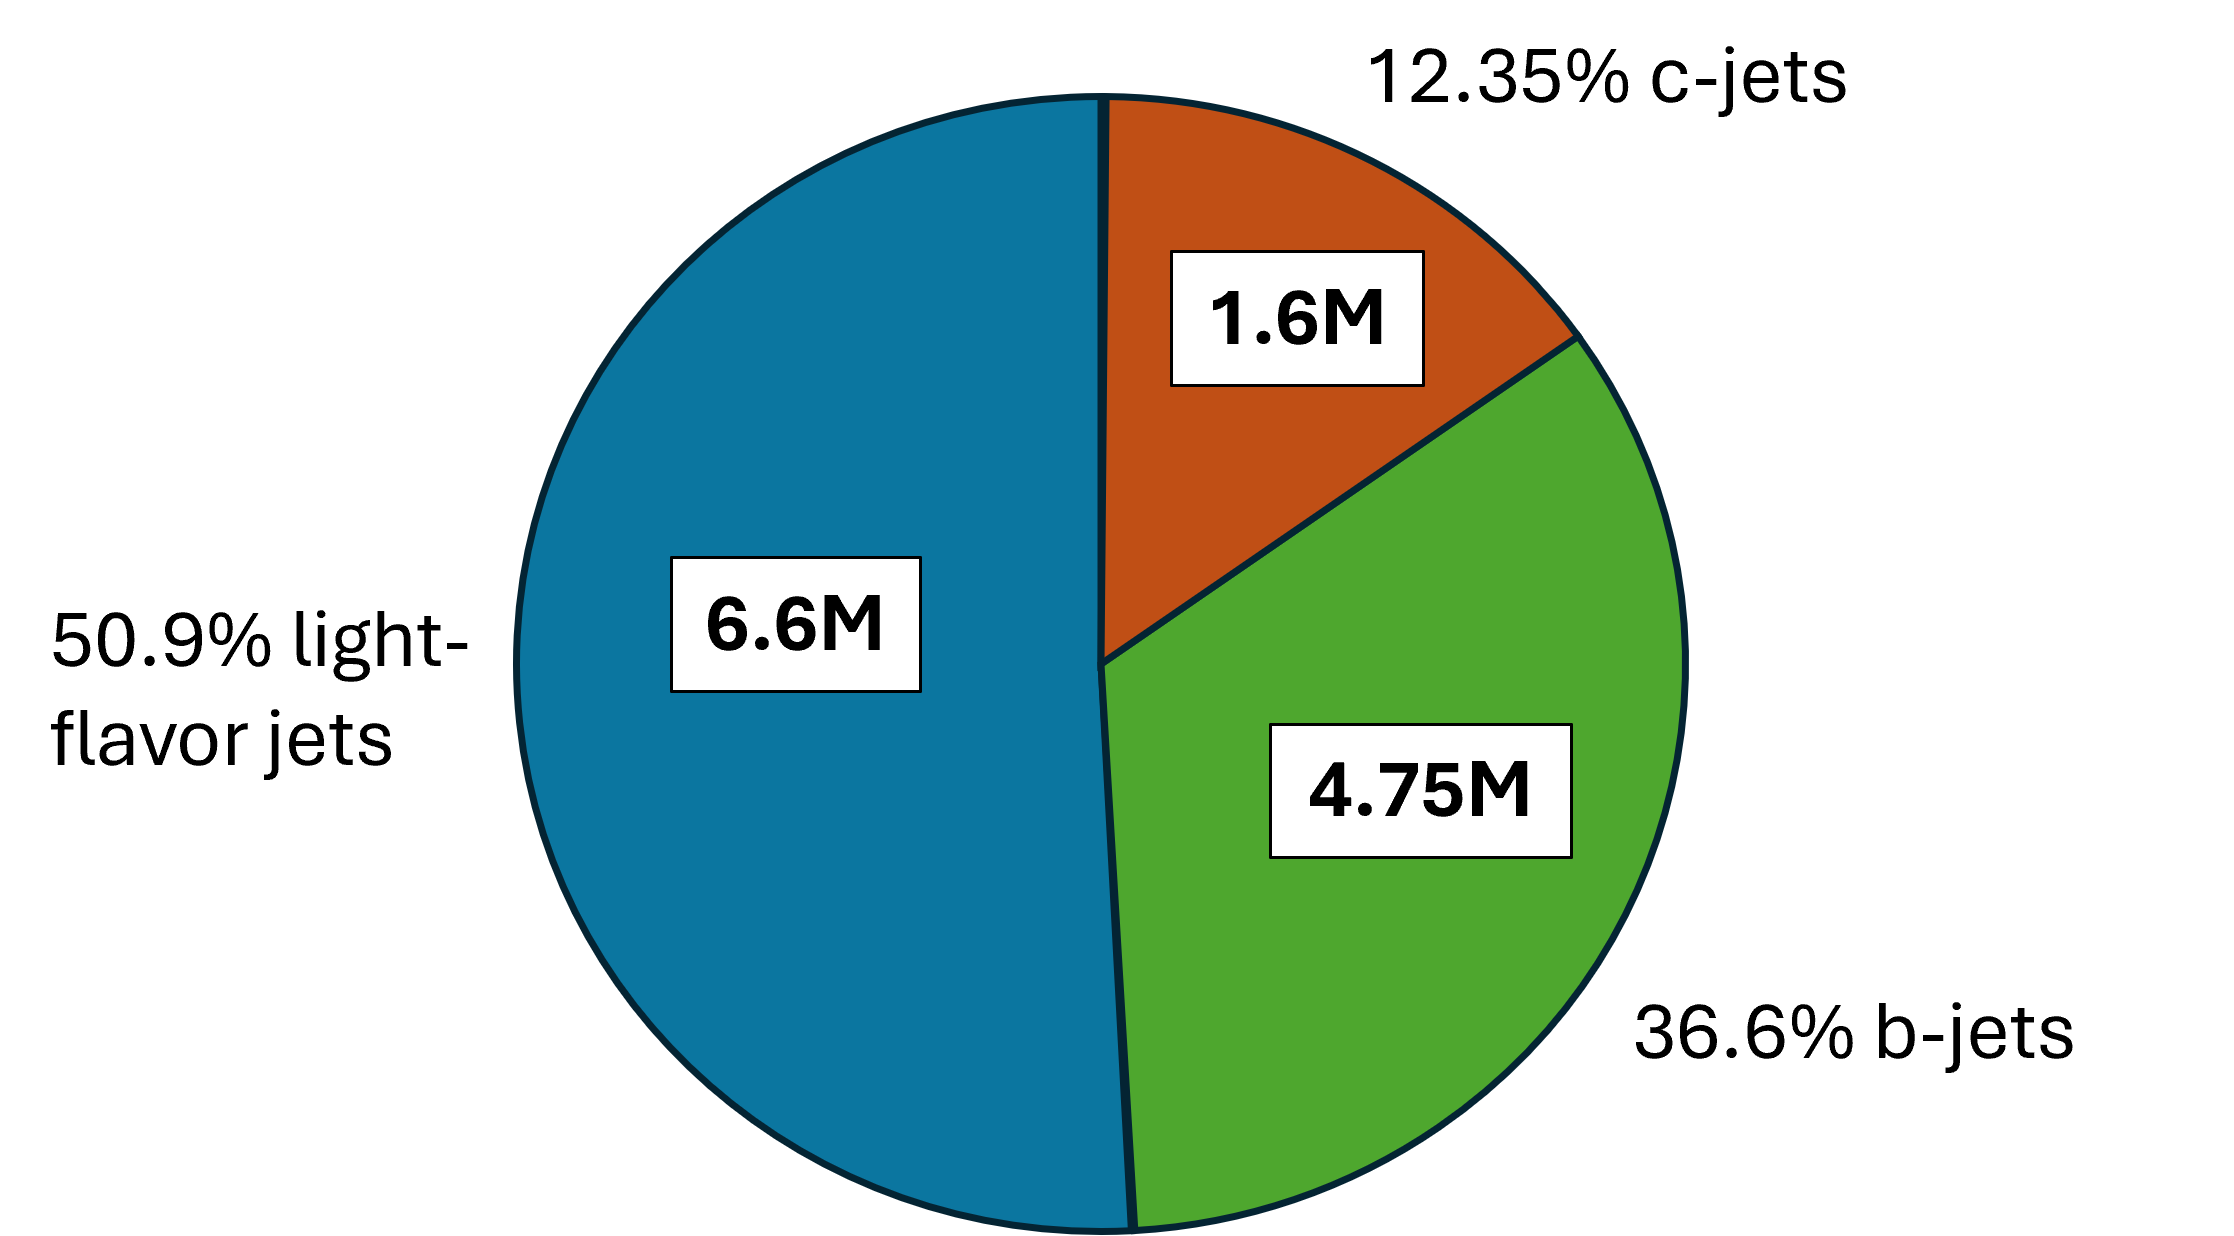
\includegraphics[scale=0.4]{figs/ch5/comp_pie.png}
    \caption{ Diagram of hadron composition in the HL-LHC MC samples.}
\label{fig:comp-pie}
\end{figure}

\hspace{-3mm}
\begin{table}[H]
    \centering 
    \begin{tabular}{ |c | c | c| c|}
        \hline
        \multicolumn{4}{|c |}{Dataset Compositions and Statistics}\\
        \hline\hline
        Dataset & Total Types of Jets & From: $t\bar{t}$ & From: $\textrm{Z}'$  \\
        \hline
        Training set & 4.75M b-jets & 4.1M & 650K \\
                     & 1.6M c-jets  & 900K & 700K \\
                     & 6.6M light-jets & 5.1M & 1.1M \\
        Validation set &    &  2.6M & 1.1M \\
        Testing sets   &    & 2.6M  & 1.1M  \\
        \hline
        \hline
        \multicolumn{2}{|c|}{PDF Resampling Method} & \multicolumn{2}{|c|}{Count Resampling Method} \\
        \hline
        \multicolumn{2}{|c|}{15M Training Jets} & \multicolumn{2}{|c|}{4.8M Training Jets} \\
        \hline
    \end{tabular}
    \caption{Dataset statistics used for training DL1d for the HL-LHC}
    \label{tab:training-stats}
\end{table}

\subsection{Training DL1d}

The training of the DL1d tagger for the \gls{hllhc} is only preliminary where the final version will have more of a dedicated optimization and increased statistics. The \gls{dips} tagger that is 
used as input for this preliminary version of DL1d for Upgrade was trained by a fellow graduate student and was trained using two electron selections. Within \gls{atlas}, four fixed values
of the electron discriminant are defined (similar to the \gls{wp} defined for b-tagging).
These \gls{wp}s for the electron selection cuts are referred to as \textit{VeryLoose}, \textit{Loose}, \textit{Medium}, \textit{Tight} cuts. These cuts are set by the efficiencies for 
identifying a prompt electron with $\textrm{E}_{\textrm{T}}$ = 40 GeV are 93\%, 88\%, 80\% for \textit{Loose}, \textit{Medium}, \textit{Tight} respectively \cite{ele-cut}. One \gls{dips} model contains a tighter 
\gls{wp} selection cut, and the other a loose \gls{wp} selection cut.  Therefore, four DL1d models are trained in total, two models trained using both of these cuts and 
being resampled via the count method and the other two using the PDF method. The DL1d architecture follows the deep feed-forward architecture shown in Figure \ref{fig:dl1-arch} but with specified nodes.
A diagram showing the specified node architecture can be seen in Figure \ref{fig:dl1d-arch}.

\begin{figure}[h]
    \centering
    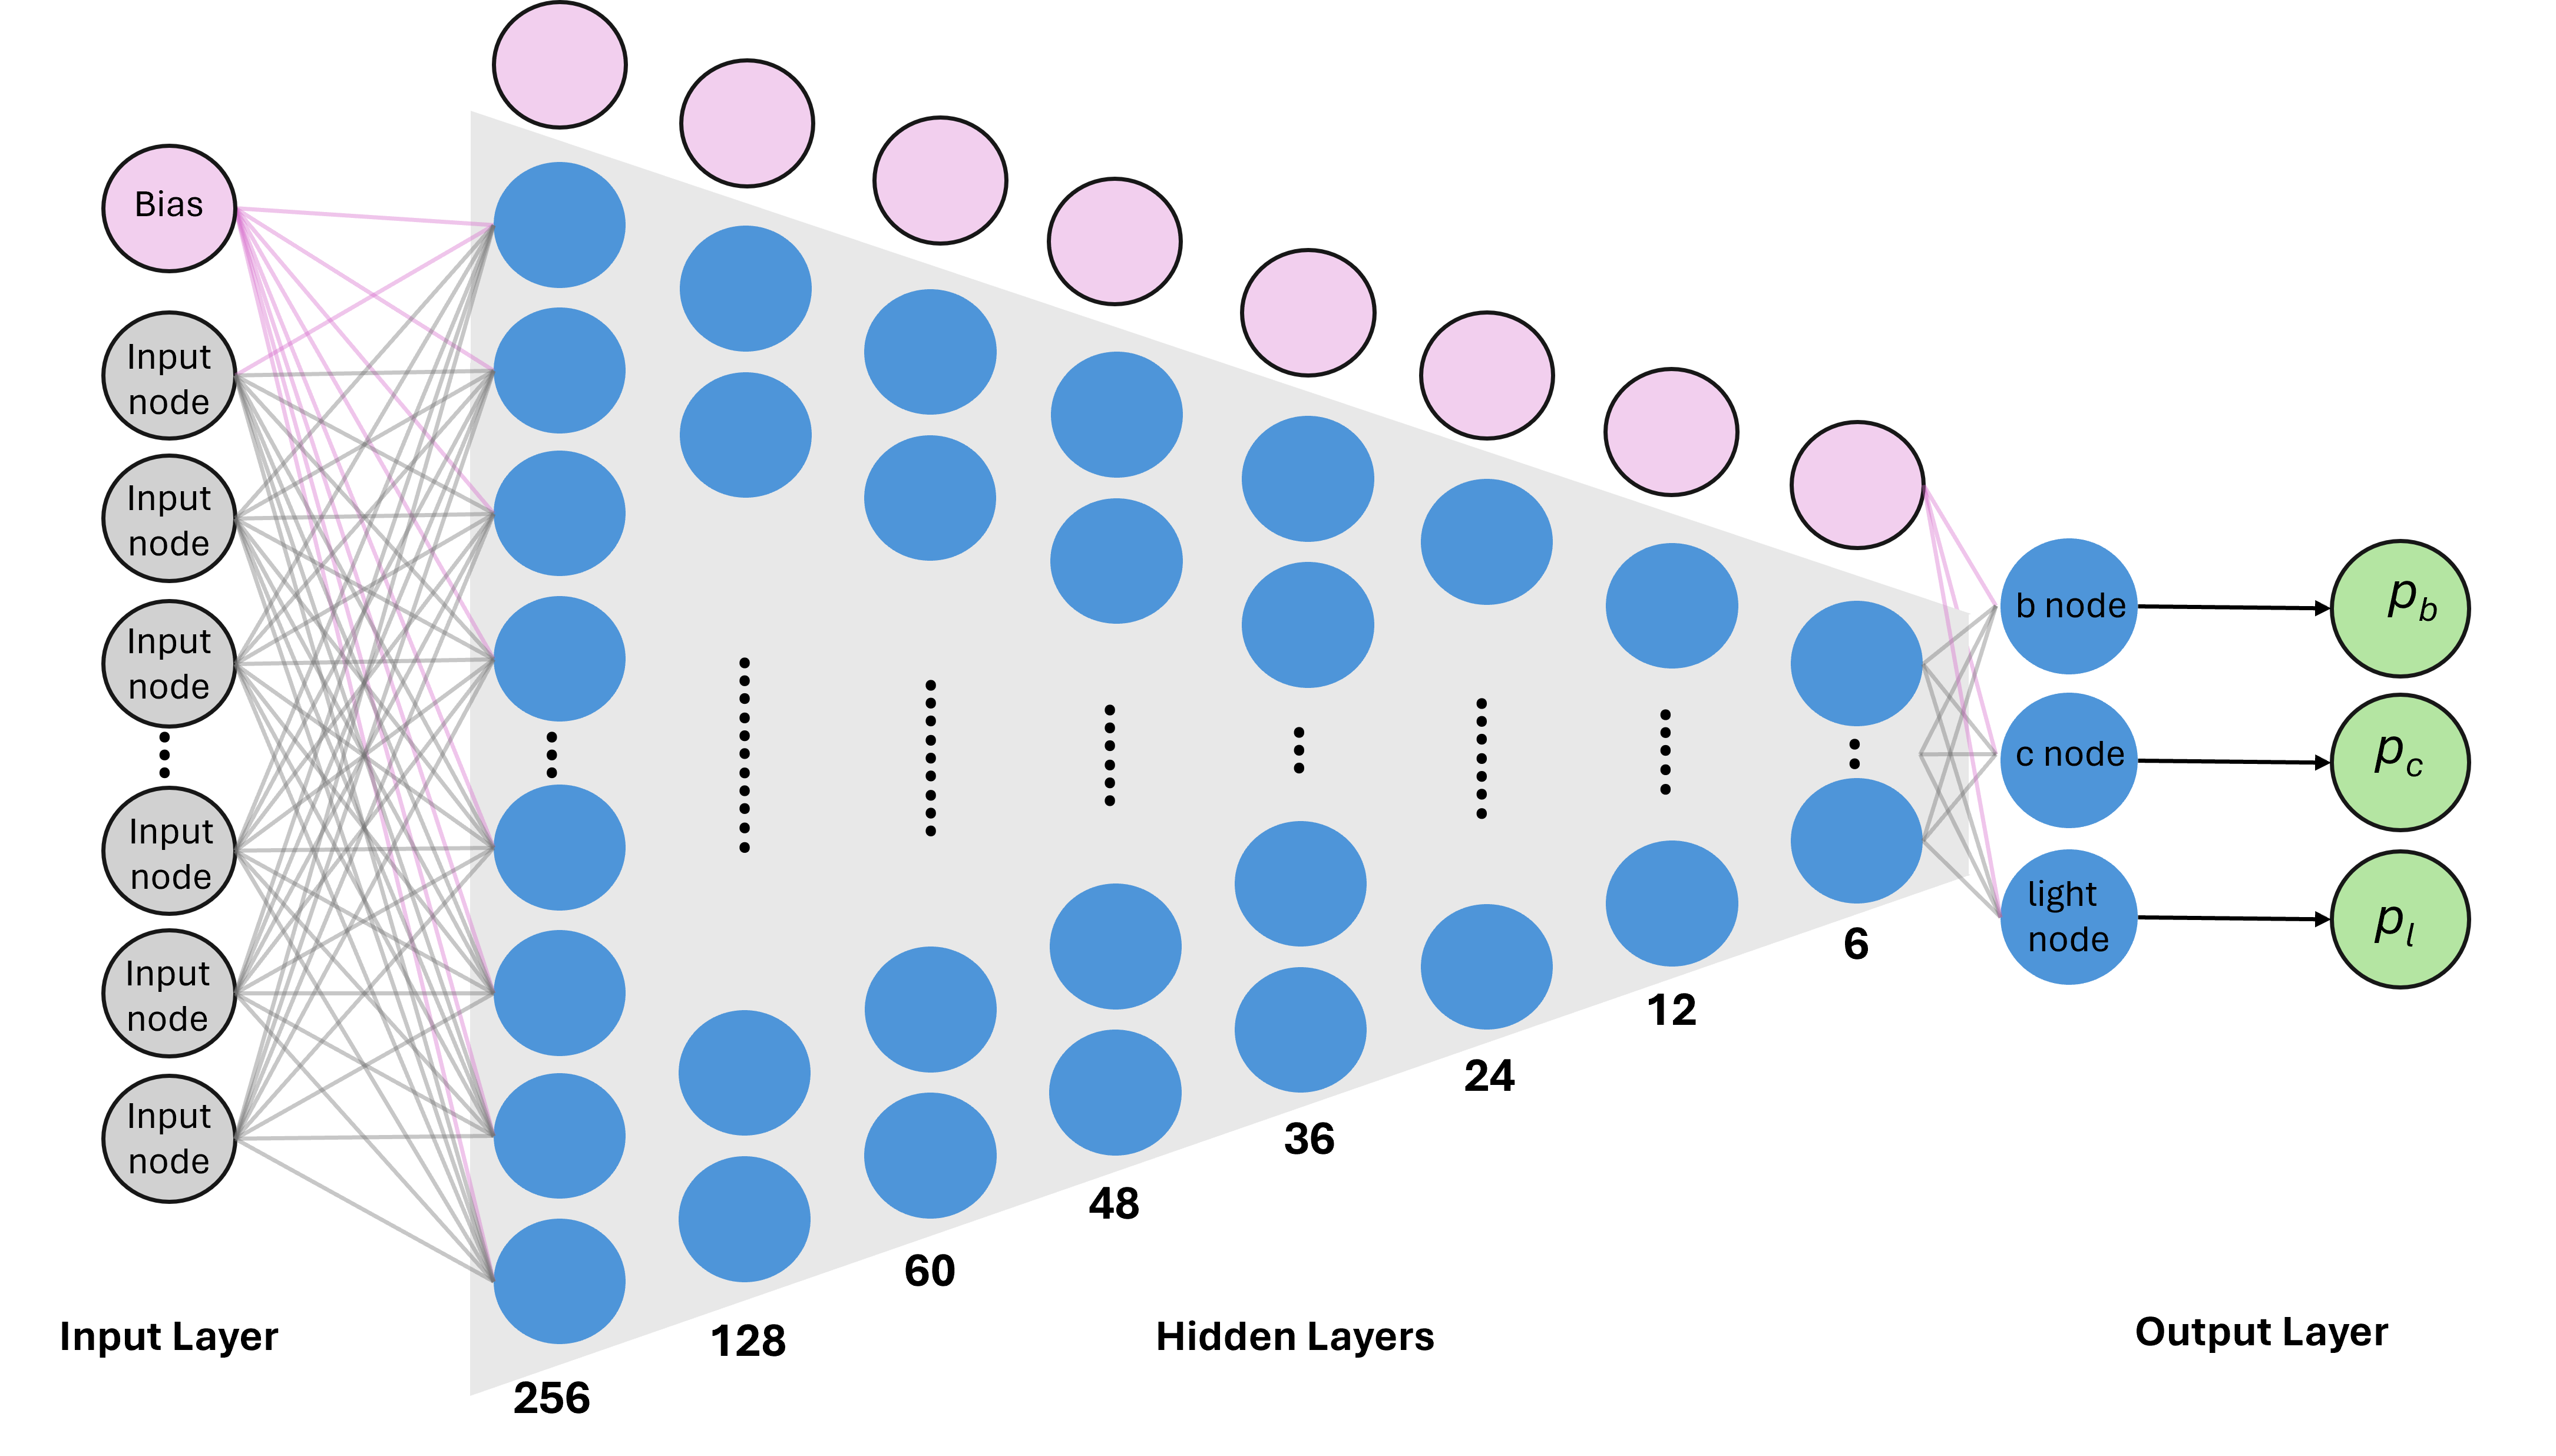
\includegraphics[scale=0.5]{figs/ch5/dl1d-arch.png}
    \caption{ Deep feed-forward architecture used for preliminary Upgrade DL1d model.}
\label{fig:dl1d-arch}
\end{figure}

Using the loss function described in Eq. \ref{eq:5.4}, the loss value is recorded per training epoch and plotted in Figure \ref{fig:vepoch} while 
also showing the loss of the associated \gls{dips} model used in the DL1d architecture. The loss is shown for the $t\bar{t}$ sample,
$\textrm{Z}'$ sample and the combined hybrid sample. Since the training is done on the hybrid sample, the loss function converges 
much quicker than just on the single samples. Figures \ref{fig:vepocha} and Figure \ref{fig:vepochb} shows the loss per epoch for both the PDF method and Count method, revealing 
that loss convergence stabilizes faster in the PDF method than the count. This is due to the increase of statistics, letting the model 
training being able to reliably find underlying patterns at a faster rate. Figures \ref{fig:vepochc} and \ref{fig:vepochd} shows the light-jet rejection rate with 
respect to the training epoch. This reveals the increase of effectiveness between the \gls{dips} model and the DL1d. Adding jet 
kinematic information from the baseline taggers to the underlying track structures from \gls{dips} massively increases light-jet 
rejection rate. Using the PDF resampling increases this rejection rate as seen between plots (c) and (d) in Figure \ref{fig:vepoch}. The convergence 
in the undersampling method Count takes about 100 more epochs, substantiating that the PDF resampling method is the superior approach. All 
these figures used the 77\% \gls{wp} for b-tagging. 


\begin{figure}[H]
    \centering
    \begin{subfigure}{0.45\textwidth}
        \centering
        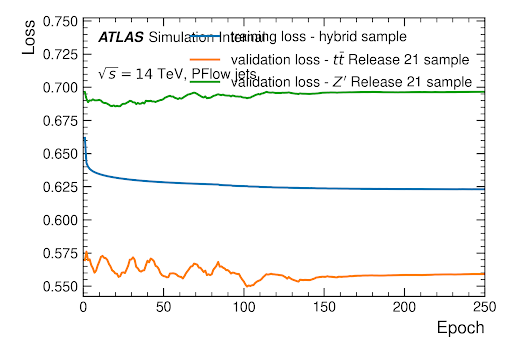
\includegraphics[width=\textwidth]{figs/ch5/lossvepoch_pdf.png}
        \caption{Loss per training epoch using PDF}
        \label{fig:vepocha}
    \end{subfigure}
    \begin{subfigure}{0.45\textwidth}
        \centering
        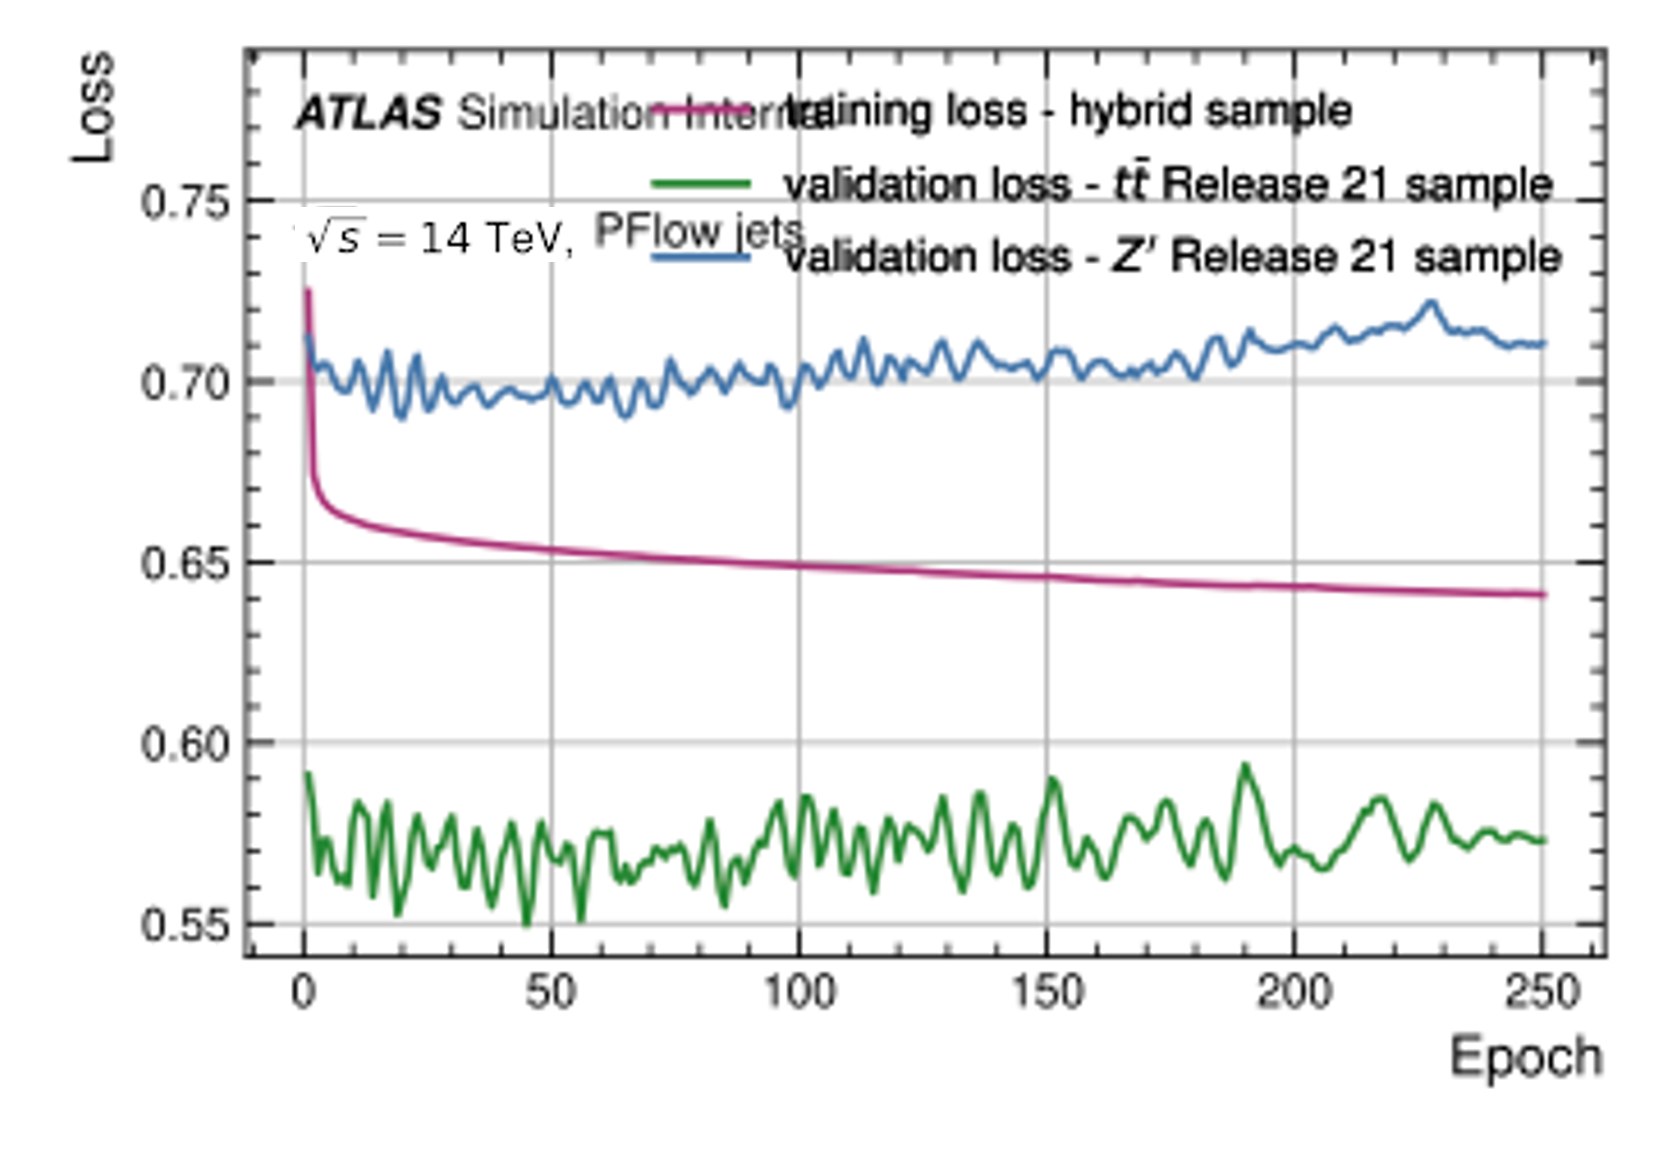
\includegraphics[width=\textwidth]{figs/ch5/lossvepoch_count.png}
        \caption{Loss per training epoch using Count}
        \label{fig:vepochb}
    \end{subfigure}
    \begin{subfigure}{0.45\textwidth}
        \centering
        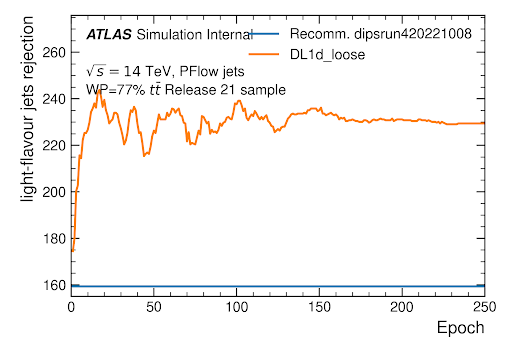
\includegraphics[width=\textwidth]{figs/ch5/rejvepoch_pdf.png}
        \caption{PDF light-jet rejection rate per epoch}
        \label{fig:vepochc}
    \end{subfigure}
    \begin{subfigure}{0.45\textwidth}
        \centering
        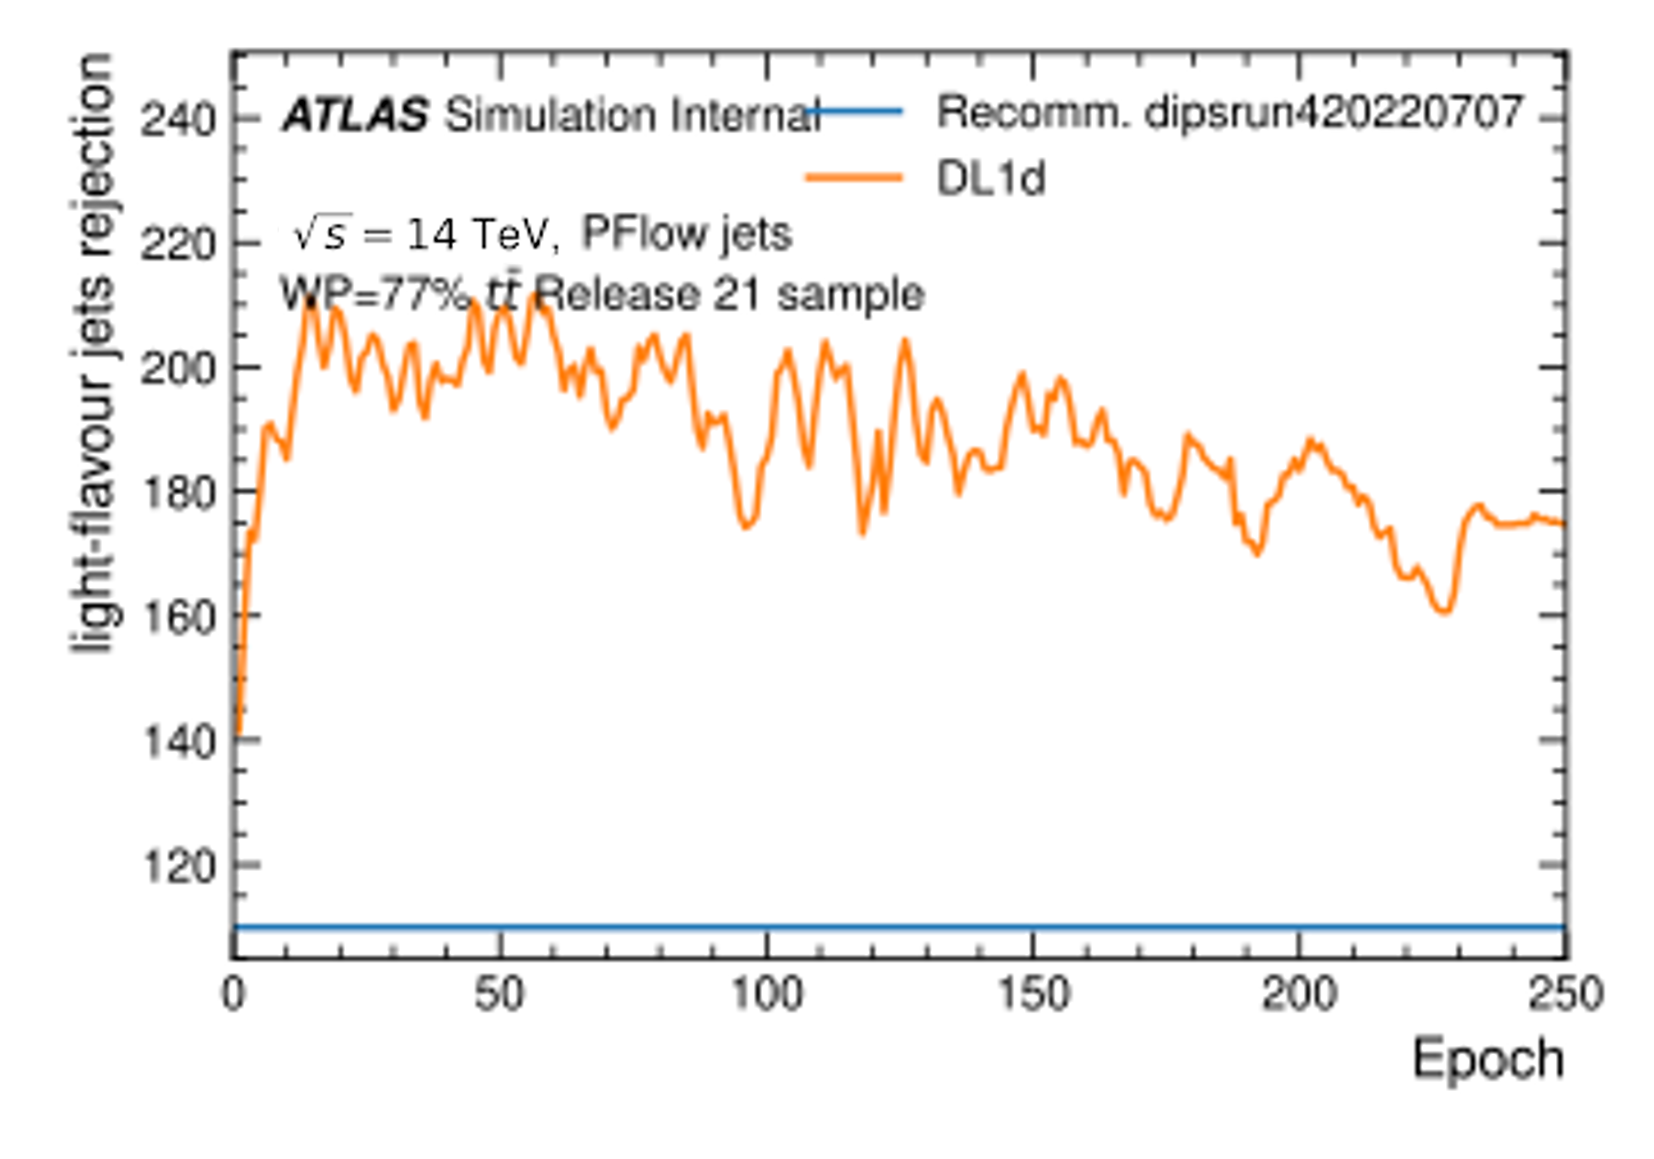
\includegraphics[width=\textwidth]{figs/ch5/rejvepoch_count.png}
        \caption{Count light-jet rejection rate per epoch}
        \label{fig:vepochd}
    \end{subfigure}
    \caption{(a) Shows loss per training epoch using the PDF method for both DL1d and its associated DIPS model using the loose electron selection cut. 
    (b) Shows loss per training epoch using the count resampling method for both DL1d and its associated DIPS model using the loose electron selection cut.
    (c) Shows the light-jet rejection rate per training epoch using the PDF method. DL1d shows rejection at a higher efficiency. 
    (d) Shows the light-jet rejection rate per training epoch using the Count resampling method. DL1d outperform DIPS but does not has a lower rejection rate than using the PDF resampling method as seen in (c)}
    \label{fig:vepoch}
\end{figure}


In order to calculate the final discriminant scores, a fraction scan is implemented 
to find an effective c-jet fraction value for the float $\textrm{f}_{\textrm{c}}$ shown in Eq. \ref{eq:5.2}. Since light-jet rejection 
and c-jet rejection are both affected by the chosen floating value, it's optimized to have a balanced effect in the $t\bar{t}$ sample while 
favoring c-jet rejection in the $\textrm{Z}'$ sample. The fractions are taken at the 77\% \gls{wp}. The scan can be seen in Figure \ref{fig:cfrac}.
Table \ref{tab:c-perc} shows the actual percentage value of c-hadrons within each sample. The value of 9\% was chosen for $\textrm{f}_{\textrm{c}}$ 
and can be seen in Figure \ref{fig:cfrac} at the point marked by the red \textit{X}. 


\begin{table}[H]
    \centering 
    \begin{tabular}{ |c | c |}
        \hline
        \multicolumn{2}{|c |}{C Hadron Percentage}\\
        \hline\hline
        Dataset & percentage  \\
        \hline
        $t\bar{t}$ & 7\% \\
        $\textrm{Z}'$ & 9\% \\
        \hline
    \end{tabular}
    \caption{C-hadron percentages in both training samples prior to combining}
    \label{tab:c-perc}
\end{table}


\begin{figure}[h]
    \centering
    \subfloat[\centering ]{{\includegraphics[scale=0.35]{figs/ch5/cfrac_ttbar.png}}}%
    \qquad
    \subfloat[\centering ]{{\includegraphics[scale=0.35]{figs/ch5/cfrac_zp.png}}}%
    \caption{ C-jet fraction scans for the float value $\textrm{f}_{\textrm{c}}$. The balancing value chosen is marked by \textit{X} on both plots.
    The chosen value is 0.09, balancing the light-jet rejection and c-jet rejection in the $t\bar{t}$ sample while favoring c-jet rejection in the $\textrm{Z}'$ sample.}
\label{fig:cfrac}
\end{figure}

Since four models were trained using both resampling methods (PDF and Count) while using two different \gls{dips} models that use different electron cuts, they had to be compared to see which 
model outperforms the other three. While holding the optimized value of $\textrm{f}_{\textrm{c}}$ = 0.09, the b-jet tagging efficiency was checked for all the models. Figure \ref{fig:dl1d-comp} shows a Receiver Operating Characteristic (\gls{roc}) curve. This shows background rejection vs b-tagging efficiency. The goal for these models is to have the highest rate of b-tagging efficiency while 
rejecting the most amount of background. The bottom two plots below the \gls{roc} curve are two ratio plots showing the efficiency of the DL1d models with respect to the DL1d using the Count 
resampling method. The left plot validates the models on the $t\bar{t}$ sample while the right validates them on the $\textrm{Z}'$ sample. It's quite noticable on the $t\bar{t}$ sample plot that 
using the loose electron cut dramatically increases the DL1d performance b-tagging efficiency. As seen in pink on the right plots in Figure \ref{fig:dl1d-comp}, the model DL1d + the loose electron cut \gls{dips} 
model outperforms the other three while being comparable in the $t\bar{t}$ plot on the left. Therefore, the DL1d model with the loose electron selection cut was taken as the best model and was used 
in the following comparison plots for the rest of this section.

\begin{figure}[h]
    \centering
    \subfloat[\centering ]{{\includegraphics[scale=0.43]{figs/ch5/rejveff_ttbar.png}}}%
    \qquad
    \subfloat[\centering ]{{\includegraphics[scale=0.43]{figs/ch5/rejveff_zp.png}}}%
    \caption{ Comparison plots of all four DL1d trained models. Plot (a) shows the performance of each model using the $t\bar{t}$ sample. Both loose electron WPs outperform the tight WP. Plot (b) shows
    all four DL1d models validated on the $\textrm{Z}'$ sample. Again, both loose electron WPs models outperform the tight WPs while the PDF resampling method (pink) outperforms the Count method (green).
    The loose DL1d model using the PDF resampling method was chosen to be the superior trained model. }
\label{fig:dl1d-comp}
\end{figure}

Once the optimum model was chosen, the next step was to check on how the performance of it compares to the baseline \gls{dips} model. It is expected for the DL1d model to greatly outperform 
the \gls{dips} model simply due to the fact that the jet kinematics are added after the training of \gls{dips}, increasing the underlying pattern recognition from the excess of available information. 
This performance can be seen in Figure \ref{fig:dl1d-dips-comp}. As expected, the DL1d model outperforms the baseline \gls{dips} model by approximately 25\% in c-jet rejection vs b-tagging efficiency.

\begin{figure}[h]
    \centering
    \includegraphics[scale=0.75]{figs/ch5/rejveff_dl1dcdips.png}
    \caption{ Comparison plot for the DL1d model and the baseline DIPS. DL1d outperform DIPS as expected. The c-jet fraction for the DIPS model was taken to be $\textrm{f}_{\textrm{c}}$ = 0.17 whereas 
    this fraction was $\textrm{f}_{\textrm{c}}$ = 0.09 as previously stated. }
\label{fig:dl1d-dips-comp}
\end{figure}

Just as in testing the model's b-tagging efficiency, the c-tagging efficiency can also be checked using the discriminant seen in Eq. \ref{eq:5.2}. The following plots show the performance of both 
the DL1d and the baseline \gls{dips} tagger for c-tagging efficiency. The DL1d tagger outperforms the \gls{dips} as expected just as in the b-tagging study. For these plots, the \gls{hgtd} sample 
was used as listed in Table \ref{tab:dl1-samples}. Two performances are shown for two different floating b-jet fractions $\textrm{f}_{\textrm{b}}$ as seen in Eq. \ref{eq:5.2}. The left plot 
has a floating b-jet value of $\textrm{f}_{\textrm{b}}$=0.24 and the right plot has a value of $\textrm{f}_{\textrm{b}}$=0.45.

\begin{figure}[h]
    \centering
    \subfloat[\centering ]{{\includegraphics[scale=0.45]{figs/ch5/brej24c.png}}}%
    \qquad
    \subfloat[\centering ]{{\includegraphics[scale=0.45]{figs/ch5/brej45c.png}}}%
    \caption{ Light-jet rejection vs b-jet rejection (c-tagging). The left plot has a floating fraction of $\textrm{f}_{\textrm{b}}$=0.24 where as the right has $\textrm{f}_{\textrm{b}}$=0.45. The DL1d
    tagger outperforms DIPS as expected. The small HGTD sampled as listed in Table \ref{tab:dl1-samples} was used. }
\label{fig:dl1d-ctag}
\end{figure}

This DL1d tagger was the first of its kind to be trained on samples with the geometry of \gls{atlas} in Run 4. With the increase of luminosity within the \gls{hllhc} and the upgrades in timing 
resolution and granularity within the \gls{itk} and \gls{hgtd}, tagging efficiencies is expected to increase. It has proved to be difficult to train a preliminary tagger to outperform the current 
state-of-the-art taggers. Though, at the current state, this is to be expected for several reasons. One would expect the tagging efficiency to increase with the amount of available statistics to train on.
This preliminary DL1d using Upgrade samples had a total of $\approx$15 million jets to train on that include jets between the newly included eta range of 2.4 $<|\textrm{η}|<$ 4.0 (total range of 0 $<|\textrm{η}|<$ 4.0) 
which may not include well resolved jets. The current state-of-the-art DL1d tagger was trained using 120 million jets simulated using Run 2 \gls{atlas} geometry with well resolved jets between the 
eta range of  0 $<|\textrm{η}|<$ 2.4. The comparison of these two versions of DL1d can be seen in Figure \ref{fig:dl1d-mv2-comp}. This figure also includes the old high-level tagger of \gls{mv2} that was validated on 
samples with the inclusive eta range of 0 $<|\textrm{η}|<$ 4.0. In this comparison \gls{roc} plot, it is seen that the DL1d for Run 2 outperforms the preliminary DL1d for Upgrade up to the 77\% \gls{wp} but starts to under perform at the 85\% \gls{wp} in the light-jet rejection. This result is highly promising knowing the robustness of the Run 2 version. If a more refined DL1d for Upgrade model is trained using 
an increase in statistics, it would be expected to outperform the Run 2 DL1d at the 77\% \gls{wp}.

\begin{figure}[h]
    \centering
    \includegraphics[scale=0.75]{figs/ch5/rejveff_mv2.png}
    \caption{ ROC curve comparing the performance of the DL1d for Run 4, the current version of DL1d used for Run 2 and the MV2 high-level tagger.}
\label{fig:dl1d-mv2-comp}
\end{figure}

Adding the newly available eta region of 2.4 $<|\textrm{η}|<$ 4.0 through the calculated power of the \gls{itk} detector has physicists excited about the new 
aspects that this adds to their analyses and possible innovations in the future. Though, in order to effectively probe this region, the available \gls{ftag}
high-level taggers must be trained with robustness. Due to the decreasing resolution as particles become highly boosted in a more forward region of the detector,
it is expected for particle tagging efficiency to drop. Thus, requiring newer innovative tools and techniques to be implemented with the hopes to obtain the maximum efficacy of this new phase space. The high-level tagger DL1d has been state-of-the-art through the end of Run 2 and into Run 3 of the \gls{atlas} detector's 
campaign lifetimes. The question is how well will this tagger perform during Run 4 within the extended eta region. Figure \ref{fig:dl1d-eta-comp} shows its current performance 
in increasing eta intervals of one. The performance in the highly boosted region between 3 $<|\textrm{η}|<$ 4.0 shows the poorest performance but this is 
to be expected. The Upgrade DL1d model was also validated on jets that are only contained in the eta region 0 $<|\textrm{η}|<$ 2.5 to have a proper comparison 
between the current implemented Run 2 DL1d tagger. The ratio plot on Figure \ref{fig:dl1d-eta-comp} shows the performance between these two taggers. Similar performance is seen at 
the 77\% \gls{wp} with an increasing performance above this value. This result is very promising since the Run 4 version of the DL1d tagger was trained on a 
magnitude less of statistics.
\par
Overall, this first preliminary study of the high-level tagger DL1d using samples that simulate the Upgrade geometry of the \gls{atlas} detector during Run 4 
and the first implementation of the \gls{hllhc} shows very promising results.  
There are currently active efforts to develop a new state-of-the-art high-level tagger using a graph neural network on tracking information called \gls{gn1}. 
The architecture was briefly discussed in Section \ref{sec:gn1}. Preliminary studies of this new tagger were done using the same samples that 
were used in this study of Run 4 for DL1d. The results of this study are discussed in Appendix \ref{appendix:gn1-upgrade}. As seen from the results of this \gls{gn1} tagger,
it outperforms the DL1d tagger. Due to this, a graph neural based tagger is planned to be considered the new industry used tagger after the upgrade in 2029. Therefore, 
further studies of the DL1d tagger using larger Upgrade samples is not planned for and the model trained in this dissertation will be used at the DL1d baseline model for Upgrade. 

\newpage

\begin{figure}[H]
    \centering
    \includegraphics[scale=0.75]{figs/ch5/rejveff_eta.png}
    \caption{ ROC curve showing the performance of the DL1d tagger for Upgrade in four eta intervals of one. The Run 2 DL1d is also plotted for comparison in the ratio plot on the bottom.}
\label{fig:dl1d-eta-comp}
\end{figure}

\begingroup
\clearpage% Manually insert \clearpage
\let\clearpage\relax% Remove \clearpage functionality
\vspace*{-16pt}% Insert needed vertical retraction
\chapter[SEARCH FOR NEW PHYSICS USING UNSUPERVISED MACHINE LEARNING FOR ANOMALY DETECTION]{SEARCH FOR NEW PHYSICS USING UNSUPERVISED MACHINE LEARNING FOR ANOMALY DETECTION}
\label{ch6}
\endgroup

Anomaly detection methods are in their infant stages within the \gls{hep} community. This analysis was the first published general search using an unsupervised machine learning method 
within the \gls{atlas} collaboration. This method searches for new physics in two-body invariant masses in events with a single isolated lepton using all data from Run 2 (140$\textrm{fb}^{\textrm{-1}}$)
of $\sqrt{\textrm{s}}$ = 13 TeV collision data recorded by the \gls{atlas} detector. The invariant mass distributions are a phase space defined by an unsupervised deep-learning machine learning 
algorithm called the autoencoder (\gls{ae}). The di-object invariant masses, $\textrm{m}_{\textrm{jX}}$, are constructed from a leading jet \textit{j} and \textit{X} is a second jet, a b-jet, 
lepton, or a photon. Similarly, $\textrm{m}_{\textrm{bX}}$, is looked at where \textit{b} is a b-jet and \textit{X} is a jet, b-jet, lepton or a photon, totaling in nine different invariant mass combinations.
A search for di-object resonances was applied in the 
invariant mass range between 0.3 TeV to 6 TeV. The \gls{ae} was trained using a data-driven technique, therefore did not rely on \gls{mc} calculations. The invariant masses in the outlier phase 
space was set to a 95\% confidence level upper limits on cross-section times branching ratios for the production of decays of resonances as predicted by several new physics scenarios.  

\section{Strategy}

Due to the fact that this analysis was still paving the way to normalize anomaly detection methods and techniques, a few choices were fairly ambiguous and had to be thoroughly thought through 
in order to establish credibility. This method searching for signatures of \gls{bsm} physics is model agnostic, meaning no theory for new physics influenced any of the model training and therefore 
any signatures detected is purely data-driven. The idea is to perform unsupervised training on a \gls{ml} model that will be able to detect events that differ from the ``average'' \gls{sm} events,
i.e. anomalous events. The input representation and training procedure should not bias the signatures and create artificial peaks. The strategy is this:

\begin{itemize}
    \item Prepare the events into an input feature space that is general enough to cover a large range of possible \gls{bsm} signatures while also providing an unbiased depth in data representation and 
    \item Train an optimized \gls{ml} model with metrics that can be used to define an anomaly score in order to show separation between ``average'' \gls{sm} events and outliers.
    \item Define anomalous events using a chosen anomaly score and use a cut on this score to obtain an anomalous region of interest.
    \item Study these anomaly regions (\gls{ar}s) for possible new physics signatures.
\end{itemize}

The last step suggests that new two-body states may be produced within these \gls{ar}s and can be seen as excesses in these distributions, which can be found without using any \gls{mc} simulations 
for background modeling. 

\section{Event Selection and Object Definitions}

All the data used in this analysis is originated from the \gls{atlas} detector during the Run 2 period between the years 2015 to 2018. The data was recorded during stable beam conditions 
while all relevant subdetectors were fully operational. The event candidates selected was done by either single-electron triggers or single-muon triggers which range in transverse momenta, 
transverse energy, and quality and isolation thresholds. These \gls{grl} files, datasets and used triggers can be found within the appendix section \ref{appendix:hlt-triggers-ad}.
\par
Muon and electron criteria are key to this analysis since they are the trigger for event selections. The Muon and electron selection criteria are summarized in Table \ref{tab:muon-sel} and Table \ref{tab:ele-sel}, respectively. 

\begin{table}[ht]
    \centering 
    \begin{tabular}{ |m{5cm} |m{6cm} |}
        \hline
        \multicolumn{2}{|c |}{Muon Selection}\\
        \hline\hline
        Criteria & Value \\
        \hline
        Selection WP & medium \\
        Isolation WP & PflowTight\_FixedRad \\
        Momentum Calibration & Sagitta Correction Not Used \\
        $\textrm{\textit{p}}_{\textrm{T}}$ Cut & $>$ 20 GeV \\
        $|\textrm{η}|$ Cut & $<$ 2.7 \\
        $\textrm{d}_{\textrm{0}}$ Significance Cut & $<$ 3 \\
        $\textrm{\textit{z}}_{\textrm{0}}$ Cut & $<$ 0.5 \\
        \hline
    \end{tabular}\hfill
    \caption{Muon selections for this analysis}
\label{tab:muon-sel}
\end{table}

\begin{table}[ht]
    \centering 
    \begin{tabular}{ |m{5cm} |m{6cm} |}
        \hline
        \multicolumn{2}{|c |}{Electron Selection}\\
        \hline\hline
        Criteria & Value \\
        \hline
        Pseudorapidity Range & ($|\textrm{η}|\ < \ $1.27) || (1.52 $< \ |\textrm{η}| \ <$ 2.47) \\
        Energy Calibration & ``es2018\_R21\_v0'' (ESModel) \\
        Transverse Momentum &  $\textrm{\textit{p}}_{\textrm{T}} \ >$ 20 GeV\\
        Track-to-Vertex Association & |$\textrm{d}_{\textrm{0}}^{\textrm{BL}}(\sigma)| \ <$ 5\\
                                    & |$∆\textrm{z}_{\textrm{0}}^{\textrm{BL}}sin\theta| \ <$ 0.5 mm\\
        Selection WP  & Tight \\
        Isolation WP & FCTight \\
        \hline
    \end{tabular}\hfill
    \caption{Electron selections for this analysis}
\label{tab:ele-sel}
\end{table}

\subsection{Photon Selection and Reconstruction}

Photon energy depositions are found within the \gls{ecal} which have a $\textrm{\textit{p}}_{\textrm{T}} \ >$ 20 GeV and have $|\textrm{η}|\ < \ $2.37. The transition region between the \gls{ecal} and the 
barrel, 1.37 $< \|\textrm{η}|\ < \ $1.52, are excluded. There are two types of photons, one is a converted photon which are formed from \gls{ecal} clusters which are matched to a conversion vertex 
and then there are unconverted photons which are clusters that are not matched to any vertex. The energy depositions, i.e. shower shapes, undergo a strict criteria to pass selections that 
correspond to the \textit{Tight} identification \gls{wp} and \textit{Tight} isolation. These photons are used in the invariant masses, $\textrm{\textit{m}}_{\textrm{j}\gamma}$ and 
$\textrm{\textit{m}}_{\textrm{b}\gamma}$. 

\subsection{Jet Definition and Selection}

Jets are constructed using the anti-$\textrm{\textit{k}}_{\textrm{T}}$ algorithm with a distance parameter of R = 0.4. They are reconstructed from PFlow objects. In order to suppress pile-up, the \gls{jvt} technique is used, 
requiring at least 60\% of the tracks momentum to be associated with the hard scatter. The \gls{jvt} algorithm is applied to jets with $\textrm{\textit{p}}_{\textrm{T}} \ <$ 60 GeV and $|\textrm{η}|\ < \ $ 2.4.
The final jet cut selection requires $\textrm{\textit{p}}_{\textrm{T}} \ >$ 20 GeV and $|\textrm{η}|\ < \ $ 2.4. Table \ref{tab:jet-sel} shows the definition of jets used in this analysis. 

\begin{table}[ht]
    \centering 
    \begin{tabular}{ |m{5cm} |m{6cm} |}
        \hline
        \multicolumn{2}{|c |}{Jet Reconstruction Parameters}\\
        \hline\hline
        Parameter & Value \\
        \hline
        algorithm & anti-$\textrm{\textit{k}}_{\textrm{T}}$ \\
        R-parameter & 0.4 \\
        input constituent &  PFlow \\
        Analysis Release Number  & 21.2.177 \\
        \hline
        \multicolumn{2}{|c|}{Selection Requirements}\\
        \hline\hline
        Observable & Requirement \\
        \hline
        Jet Cleaning & LooseBad \\
        BatMan Cleaning & No \\
        $\textrm{\textit{p}}_{\textrm{T}}$ & $>$ 20 GeV \\
        $|\textrm{η}|$ & $<$ 2.47 \\
        JVT WP & Medium \\
        \hline
    \end{tabular}\hfill
    \caption{Jet definitions used in this analysis}
\label{tab:jet-sel}
\end{table}

\subsection{B-jet Selection}

The AntiKt4EMPFlow b-jets were selected from the 77\% \gls{wp} using the DL1r algorithm. The minimum jet $\textrm{\textit{p}}_{\textrm{T}}$ for pre-selection was 20 GeV. No optimizations of the 
\gls{wp}s were made based on the \gls{bsm} models used.

\subsection{Final Selection}\label{sec:final_sel}

After all the pre-selection requirements and stated in the previous sections were made, a final selection is applied to define our signal region. This region requires at least one 
isolated lepton with $\textrm{\textit{p}}_{\textrm{T}} \ >$ 60 GeV and at least one jet with $\textrm{\textit{p}}_{\textrm{T}} \ >$ 30 GeV. The pseudorapidity requirement is $|\textrm{η}|\ < \ $ 2.4 for jets, 
$|\textrm{η}|\ < \ $ 2.5 for muons and $|\textrm{η}|\ < \ $ 2.47 for electrons. The FCTight and PFlowTight isolation \gls{wp}s were used for electrons and muons respectively. This tight 
criteria imposed on leptons allows for consistent candidate definitions. The invariant masses, $\textrm{m}_{\textrm{jj}}$, $\textrm{m}_{\textrm{jb}}$, $\textrm{m}_{\textrm{bb}}$, are reconstructed 
using two jets from each event, either with a leading and sub-leading (b-)jets, or with a b-jet or anti-b-jet. The minimum value of the invariant mass was chosen to be 400 GeV. This decision 
was made, in short, because the lepton cut of $\textrm{\textit{p}}_{\textrm{T}} \ >$ 60 GeV is expected to distort the mass distributions of $\textrm{m}_{\textrm{je}}$ and $\textrm{m}_{\textrm{jμ}}$ 
between the range of 200 and 400 GeV. 

\section{Monte Carlo Simulations}

Even though this technique is considered a data-driven approach in order to not rely on \gls{mc} simulations. Simulations were still used to describe the background hypothesis for a proper 
fit procedure. \gls{mc} simulations were also produced for several benchmark \gls{bsm} models that were used to show how well the trained \gls{ae} could identify anomalous events that originate 
from new physics. A more in depth discussion on the types of \gls{mc} samples used for the background hypothesis can be found in appendix \ref{appendix:mc-ad}.

\subsection{Benchmark BSM Models}

The following \gls{bsm} models are used as benchmark signals to evaluate the efficacy of the unsupervised anomaly detection \gls{ml} model. The Feynman diagrams are shown in Figure~\ref{fig:bsm-feynman}. The motivation
of choosing these specific models are discussed in the following. 

\begin{figure}[h]
    \centering
    \begin{subfigure}[h]{0.4\linewidth}
    \includegraphics[scale=0.06]{figs/ch6/feynman/fig_01a.png}%
    \caption{Sequential Standard Model}
    \end{subfigure}
    \hfill
    \begin{subfigure}[h]{0.4\linewidth}
    \includegraphics[scale=0.06]{figs/ch6/feynman/fig_01b.png}%
    \caption{Simplified DM Model}
    \end{subfigure}
    \hfill
    \begin{subfigure}[h]{0.4\linewidth}
    \includegraphics[scale=0.06]{figs/ch6/feynman/fig_01c.png}%
    \caption{Radion Model}
    \end{subfigure}
    \hfill
    \begin{subfigure}[h]{0.4\linewidth}
    \includegraphics[scale=0.06]{figs/ch6/feynman/fig_01d.png}%
    \caption{Composite-lepton Model}
    \end{subfigure}
    \hfill
    \begin{subfigure}[h]{0.4\linewidth}
    \includegraphics[scale=0.16]{figs/ch6/feynman/fig_01e.png}%
    \caption{Charged Higgs Model}
    \end{subfigure}
    \hfill
    \caption{ Feynman diagrams of the benchmark BSM models.}
\label{fig:bsm-feynman}
\end{figure}

\subsection{Sequential Standard Model}

The Sequential Standard Model (\gls{ssm}) is an extended gauge model~\cite{ssm} which proposes heavy gauge bosons which are commonly denoted as $\textrm{W}'$ and $\textrm{Z}'$. 
The emission of a $\textrm{W}$ boson was considered from the s-channel production

\begin{equation}\label{eq:6.1}
	qq \rightarrow \textrm{W}' \rightarrow \textrm{W Z}' \rightarrow (\textrm{l}\nu)(\textrm{qq})
\tag{6.1}
\end{equation}

where $\textrm{Z}'$ is a new dijet resonance that is produced in association of the W boson~\cite{Zp}. The branching ratio $\textrm{W}'$ to $\textrm{Z}'\textrm{W}$ was set to 50\%, 
while 100\% branching from $Z\to jj$ was set to increase the efficiency of \gls{mc} production. 

\subsection{Simplified Dark Matter Model}

The simplified dark matter (\gls{dm}) models contain one or more stable, long-lived \gls{dm} particle along with an unstable mediator particle that interacts between \gls{dm} and 
the \gls{sm}. The model used in this analysis consists of a single spin-1 mediator denoted as $\textrm{Z}'$ created through a new U(1) gauge symmetry. The final states contain 
one or more leptons/

\subsection{Kaluza-Klein Bosons Decaying to Radions}

In order to solve the elector-weak hierarchy problem and flavor structure origin, some \gls{bsm} theories predict warped higher dimensional compactifications with bulk \gls{sm}. 
In the model used for this analysis, a Kaluza-Klein (\gls{kk}) excitation gauge boson may decay into a particle called the radion and a \gls{sm} gauge boson~\cite{wkk1,wkk2}. 

\begin{equation}\label{eq:6.2}
\textrm{Wkk} \to \textrm{W} + \varphi \to \textrm{l}\nu + \textrm{gg}  
\tag{6.2}
\end{equation}

where $\textrm{Wkk}$ denotes the \gls{kk} boson and the $\varphi$ is a radion decaying into two gluons. 

\subsection{Composite-Lepton Model}

Composite resonances breaking lepton flavor universality predicts a $\textrm{Z}'$ particle that decays into a composite lepton (\textit{E}) and a \gls{sm} lepton~\cite{comp-lep}. The 
composite lepton then decays into a lepton and a Higgs boson or Z boson. 

\begin{equation}\label{eq:6.3}
\textrm{Z}' \to \textrm{l} + \textrm{E}; \textrm{E} \to \textrm{e} + \textrm{Z/h}; \textrm{Z/h} \to \textrm{q}\bar{\textrm{q}}
\tag{6.3}
\end{equation}

\subsection{Charged Higgs Model}

Many \gls{bsm} models predict the existence of a charged Higgs boson. For this analysis, the simulated process assumes the charged Higgs boson is produced along with a top quark and 
a bottom quark~\cite{ch-higg1}. It then decays itself into a top and bottom quark. In the very boosted regime, such as $\textrm{H}^{+}$ masses above 1 TeV, a b-jet and a jet originated from a top quark 
form almost back-to-back, which would be reconstructed via the $\textrm{m}_{\textrm{jj}}$ distributions. For lower, non-boosted masses, the leading and non-leading jets lead to 
an approximate invariant mass of the $\textrm{H}^{+}$ and end in a rather broad resonance due to incomplete reconstruction of the decay products. 

\section{Event Input Representation}\label{sec:evnt-input-rep}

Now that the pre-selection has been chosen, the question is how to represent this as input for a machine learning model in order to maximize underlying 
correlations and pattern recognition. The overall goal of this analysis is to find anomalous dijet resonances, but the input must ensure that the model is not biased towards 
only kinematic anomalies. The approach that was taken for this analysis was to represent the input as a matrix that contains correlations between each object within the event.
This matrix is called the Rapidity Mass Matrix, or \gls{rmm}. Figure \ref{fig:rmm} shows an example of the \gls{rmm} with two object types, jets (\textit{j}) and muons (\textit{μ}). The 
maximum amount of objects is set to \textit{N}. The position (1,1) contains the event's missing transverse energy, or \gls{met}, and is scaled by the center of mass energy (1/$\sqrt{\textrm{s}}$)
where $\sqrt{\textrm{s}}$ is the center-of-mass energy. The diagonal cells contain the ratio $e_T(i_n)$ = $\textrm{E}_{\textrm{T}}(\textrm{\textit{i}}_{\textrm{1}})$/$\sqrt{\textrm{s}}$,
where $\textrm{E}_{\textrm{T}}(\textrm{\textit{i}}_{\textrm{1}})$ is the transverse energy of a leading object \textit{i} (a jet or \textit{μ}), and transverse energy imbalances

\begin{equation}\label{eq:6.4}
\delta e_T(i_n) = \frac{E_T(i_{n-1})-E_T(i_{n})}{E_T(i_{n-1})+E_T(i_{n})}, \quad n=2,\ldots, N,  
\tag{6.4}
\end{equation}

for a given object type \textit{i}. All objects are strictly order in transverse energy, i.e. $\textrm{E}_T(i_{n-1})>\textrm{E}_T(i_{n})$. The top row are the particle's transverse masses $\textrm{M}_T(i_n)$
for two-body decays, scaled by 1/$\sqrt{s}$, i.e.  $\textrm{m}_T(i_n)=\textrm{M}_T(i_n)/\sqrt{s}$.
The upper-right quadrant shown in red are the non-diagonal values of $\textrm{\textit{m}}(i_n,j_k)=\textrm{M}_{i,n,\> j,k}/\sqrt{s}$, where $\textrm{M}_{i,n,\> j,k}$ are two-particle invariant masses. 
The first column vector s $h_L(i_n) = C (\textrm{cosh}(y)-1)$, where $y$ is the rapidity of a particle $i_n$, and $C$ is a constant defined such that the average 
values of $h_L(i_n)$ can correspond to certain algorithms that may require values to have similar weights. The values in the bottom-left quadrant highlighted in green $h(i_n,j_k)=C( \textrm{cosh}(\Delta \textrm{y} / \textrm{2}  )-\textrm{1} )$ 
are constructed from the rapidity differences $\Delta y=y_{i_k} - y_{j_n}$ between \textit{i} and \textit{j}.

\begin{figure}[ht]
    \centering
    \includegraphics[scale=0.68]{figs/ch6/rmm/RMM.png}
    \caption{ Example of the Rapidity Mass Matrix using only two objects, jets (\textit{j}) and muons (\textit{μ}).}
\label{fig:rmm}
\end{figure}

Applying this idea to this analysis expounds this example \gls{rmm} into a larger representation. In the end, nine invariant masses were studied, therefore the \gls{rmm} had to contain all the objects that were 
used in combination for the invariant masses. The total objects per event varies event to event. In order to deal with this variable sizing, the events were ``mapped'' to a fixed data-structure and therefore 
implement zero-padding for missing data. The the standard topology of reconstructed objects was used while setting a maximum number for each object. In total, up to 10 jets, 10 b-jets, 5 electrons, 5 muons, 
5 photons and \gls{met} were allowed (total of 36 objects). In order to reduce biasing the \gls{ml} model on the di-object invariant masses of interest, the values that correspond these nine invariant masses are zero-padded 
for every event. This gives us a total amount of variables to feed the model of 1287 ($\textrm{36}^{\textrm{2}}$-9=1287). Figure~\ref{fig:zero-rmm} shows an example \gls{rmm} with all indices allotted for objects to be filled and 
shown as yellow, whereas the zero-padded indices are shown in blue. The indices corresponding to the nine invariant masses of interest are removed to reduce bias. Appendix shows examples of single events converted to \gls{rmm}s.

\begin{figure}[H]
    \centering
    \includegraphics[scale=0.82]{figs/ch6/rmm/make_0removal.pdf}
    \caption{ This RMM diagram shows the indices that allow values (yellow) and the zero-padded indices (blue). The nine invariant masses of interest are removed (blue). This diagram shows the average values of cells for 10000 events. The total of non-zero variables is 1287.}
\label{fig:zero-rmm}
\end{figure}

\section{Autoencoder Training}\label{sec:ae-training}

The \gls{ae} model was trained using \texttt{TensorFlow} \cite{tensorflow} with a Keras backend \cite{keras}. The \gls{ae} architecture is a deep-learning algorithm that is used
for high-dimensionality reconstruction. The architecture is split into three parts. The first part is called the ``encoder'' which is the initial compression neurons which compresses 
the input into lower dimensionality. The second part of this architecture is referred to as the ``latent layer'' and is considered the bottleneck. This is a single layer of neurons
that holds the compressed input. The final stage of this architecture is called the ``decoder'' which decompresses the latent layer in order to reconstruct the original input. The 
neural-network of the decoder typically mirrors that of the encoder. The chosen amount of neurons should for these layers are optimized for the goal of anomaly detection.
\par
The \gls{ae}s purpose is to reconstruct its input. When the input gets compressed and then decompressed by the \gls{ae}, there is a certain amount of data lost within the process. 
This value is determined by the loss function that the model is trained to minimize. The loss function used for this model is the mean squared error function (\gls{mse}) which can be 
seen in Eq.~\ref{eq:6.5}

\begin{equation}\label{eq:6.5}
    \textrm{\textit{Loss}} = \frac{1}{\textrm{\textit{n}}} \sum_{i=1}^{n=1287} (\textrm{\textit{x}}_{\textrm{\textit{i}}}-\hat{x}_{\textrm{\textit{i}}})^{\textrm{2}}
\tag{6.5}
\end{equation}

It is known for \gls{ae}s that it's possible to have exactly zero loss when decompressing the input. This zero loss is not the goal of this architecture for the value of the loss is chosen to be the score in 
which indicates anomalous events. Therefore, the optimized architecture must have a range of loss values while maximizing the separation between \gls{sm} events and \gls{bsm} events.  The architecture topology 
studies for this optimization can be found in Appendix~\ref{appendix:ae-topo-studies}. The resulting optimized architecture chosen is seen in Table~\ref{tab:ae-arch}. The total number of trainable weights is 2,863,087,
the activation function used is the ``leakyReLU'' and the loss function is minimized by the Adam Optimizer. The reconstruction loss is used as the anomaly score. 

\begin{table}[H]
    \begin{verbatim}
        _________________________________________________________________
        Layer (type)                 Output Shape              Param #
        =================================================================
        input_1 (InputLayer)         [(None, 1287)]            0
        _________________________________________________________________
        dense (Dense)                (None, 800)               1030400
        _________________________________________________________________
        dense_1 (Dense)              (None, 400)               320400
        _________________________________________________________________
        dense_2 (Dense)              (None, 200)               80200
        _________________________________________________________________
        dense_3 (Dense)              (None, 400)               80400
        _________________________________________________________________
        dense_4 (Dense)              (None, 800)               320800
        _________________________________________________________________
        dense_5 (Dense)              (None, 1287)              1030887
        =================================================================
        Total params: 2,863,087
        Trainable params: 2,863,087
        Non-trainable params: 0
        \end{verbatim}
        \caption{Optimized Autoencoder architecture chosen for the anomaly detection analysis. More neurons may have optimized it further but was limited due to computational power.}
        \label{tab:ae-arch}
\end{table}

Figure~\ref{fig:AE-arch} shows a schematic of the nominal \gls{ae} model with a sample input and output.
1\% of \gls{atlas} Run 2 data is randomly selected from different data-taking periods were used for training. 70\% were used for training while 30\% were used for validation. Early stopping was set to 30 epochs. 
\gls{mc} samples nor labels were used for training, thus making this approach a data-driven unsupervised learning. Figure~\ref{fig:training-stats} shows the training loss per epoch for both the training and validation sets. 

\begin{figure}[H]
    \centering
    \includegraphics[scale=0.48]{figs/ch6/AE-arch.png}
    \caption{A schematic representation of the nominal AE model with an example input and its output. It's composed of three parts, the encoder which compress the data, the latent layer which acts as the bottleneck
    and the decoder which decompresses the data in order to recreate the original input. Due to this compression and decompression, data is loss via the loss function calculation. This loss is used as the anomaly score.
    When an event that is the model hasn't seen goes through, the data loss is higher and thus can be tagged as anomalous.}
\label{fig:AE-arch}
\end{figure}

\begin{figure}[h]
    \centering
    \begin{subfigure}[h]{0.45\linewidth}
    \includegraphics[scale=0.45]{figs/ch6/epoch_vs_loss.pdf}%
    \caption{Loss per epoch (linear)}
    \end{subfigure}
    \hfill
    \begin{subfigure}[h]{0.45\linewidth}
    \includegraphics[scale=0.45]{figs/ch6/epoch_vs_loss_log.pdf}%
    \caption{Loss per epoch (log)}
    \end{subfigure}
    \hfill
    \caption{Training and validation loss as a function of epochs shown both linear and log y-scale.}
\label{fig:training-stats}
\end{figure}

Training \gls{ml} models have dependencies on several factors such as random seed values used for \gls{ae} initialization, the processing computer architecture, training/validation dataset splitting, etc.
In order to accommodate for these factors, 50 separate trainings were conducted with different random seed values. Figure~\ref{fig:loss_seed} shows these 50 trainings and the validation value in which the \gls{ae} was stopped training.
The median value of this validation loss is ln(\texttt{loss}) is -10.554. The trained model that stopped at this median value then became the nominal model used for the rest of the analysis. 
The two $\pm$RMS models are used for systematic studies in Appendix~\ref{appendix:ae-systematics}. 

\begin{figure}
    \begin{center}
       \subfloat[Using 1\% of data for training] {
        \includegraphics[width=0.8\textwidth]{figs/ch6/seedAEleakyRelu800_400_200_400_800.pdf}
        }
    \end{center}
    \caption{Validation stop loss values for 50 trainings with different seeds. Seed value and corresponding loss value is shown in the legend.
    ``Alter training'' shows different randomly selected training data from full Run 2 ATLAS data. (ROC curves can be found in Appendix~\ref{appendix:ae-systematics})
    Consistent loss values were achieved among different training sets.}
\label{fig:loss_seed}
\end{figure}

The trained nominal \gls{ae} model was used to process \gls{mc} events and \gls{bsm} events and is shown in Figure~\ref{fig:plot_loss_mc}. The ln(\texttt{loss}) value is taken to show anomalous separation.
10\% of randomly chosen data events from Run 2 were used to check the loss distribution 
to ensure that there is good separation between data and \gls{bsm}. It can be seen that in both (a) and (b) in Figure~\ref{fig:plot_loss_mc} that there is good separation between \gls{sm} and \gls{bsm} events. The year 
dependence is also checked since all of Run 2 is taken over several years. Figure~\ref{fig:loss_year} shows that there is no shape dependence on data-taking years.

\begin{figure}[H]
    \begin{center}
       \subfloat[MC for autoencoder trained with 1\% of data] {
       \includegraphics[width=0.45\textwidth]{figs/ch6/ar/plot_loss_mc.pdf}
       }
       \subfloat[Data for autoencoder trained with 1\% of data] {
       \includegraphics[width=0.45\textwidth]{figs/ch6/ar/plot_loss.pdf}
       }
    \end{center}
    \caption{Distributions of the loss values for the AE trained using 1\% of data.
    (a) The loss distribution for SM and BSM models; (b) The loss distribution for 10\% and BSM models. 
    The BSM models had 20,000 generated events for each mass point in the range 0.5 -- 6 TeV. 
    The larger the mass of the resonance, the further away the line is from the data distribution.
    All the distributions are normalized to the unit area. 
    }
\label{fig:plot_loss_mc}
\end{figure}

\begin{figure}[H]
    \begin{center}
        \includegraphics[width=0.8\textwidth]{figs/ch6/logloss_log}
    \end{center}
    \caption{
        Distributions of the loss values for 10\% Run 2 data, scaled by 10 to simulate the actual expected distribution.
        Distributions from each data taking year are shown as well (without multiplying by 10).
        To quantify the difference, the  AE value between individual-year and all-year shapes are computed; they are found to be 'Data 15': 0.485, 'Data 16': 0.491, 'Data 17': 0.505, 'Data 18': 0.502.
        Ratio pad shows the per year shape over full data (note that colors may not be precisely matched).
        They are all close to 0.5, suggesting that different data-taking conditions (e.g.\ pile-up) do not have a large impact on the method.
    }
\label{fig:loss_year}
\end{figure}

\subsection{Determination of Anomaly Region}

The definition of an anomaly region (\gls{ar}) is ambiguous and can be determined depending on the logical needs of the analysis. Within this analysis, the decision was based 
on the example \gls{bsm} models using their theoretical cross-sections times their branching ration (after their acceptances time efficiency corrections). 
The $\sigma \times BR \times Acc  \times  Eff$ were calculated for these models and can be seen in Table~\ref{tab:bsm-cross}. The range 
of these values are within a few hundredths to a few pico-barn. Three \gls{ar}s were defined to ensure sensitivity to a wide range of \gls{bsm} models. These three regions are 
event count bases ranging from 10 pb to 0.1 pb. 

\begin{itemize}
    \item \textbf{10 pb region:} This 10 pb \gls{ar} corresponds to 10 pb $\times \textrm{140} \textrm{fb}^{\textrm{-1}}$=1.4M events. This region has the largest acceptance 
    and is a reasonable choice for many models with leptons in the final state.
    \item \textbf{1 pb region:} This 1 pb \gls{ar} corresponds to 0.14M events of data. This region is less sensitive due to the decrease in statistics but it was expected  
    that the same fit function as the 10 pb \gls{ar} could be used. This assumption is justified since this region has less events and therefore an equation with the same 
    amount or less parameters as the first region should work.
    \item \textbf{0.1 pb region:} This is the third and last \gls{ar} definition and only corresponds to 14K events. This region was included since it corresponds to the upper 
    bound on published experimental limits for dijet mass (including masses with associated lepton or photons). The same fit function will be used for this region as was 
    used in the previous regions.
\end{itemize}    

Since these \gls{ar}s were defined using a count-based assumption, it was possible to define the anomaly score cut numerically. The values were found scanning the 
amount of events bin by bin on the log(\texttt{loss}) anomaly score distribution. The cut values for the 10 pb, 1 pb and the 0.1 pb \gls{ar}s are -9.10, -8.00 and -6.5 respectively and be seen within Table~\ref{tab:test-score-cut}.

\newpage

\begin{table}[H]
    \centering
    \begin{small}
    \begin{tabular}{ |m{2cm} |m{4cm} |m{7cm} |m{2cm} |}
        \hline
        \multicolumn{4}{|c |}{Theoretical Cross Sections times Branching ratios for BSM Models}\\
        \hline
        $\sigma \times \mathrm{BR}$ (pb) & $\sigma \times \mathrm{BR}  \times  Acc  \times  Eff$ (pb) & Model & Reference \\
        \hline\hline
            10       & 2.5                 &  Sequential Standard Model  &  ATLAS  \cite{dijet-res}        \\ 
            1.5      & 0.2                 &  Charged Higgs (hMSSM, $\tan(\beta)=1$)     &   ATLAS  \cite{dijet-res}       \\
            6        & 0.3                  &   Charged Higgs (hMSSM, $\tan(\beta)=0.5$)       &    ATLAS \cite{dijet-res}       \\                     
            0.5      & 0.14                  &   Simplified dark matter model        &    ATLAS  \cite{dijet-res}       \\
            8 (extr) & 1 (extr)           &   Composite lepton model (E=250 GeV) & ATLAS \cite{iso-lep-res}    \\ 
            1.5      & 0.4 (extr)           &   Composite lepton model (E=500 GeV) & ATLAS  \cite{iso-lep-res}    \\
            0.12     & 0.05               &   Technicolor model       &    ATLAS \cite{dijet-res}       \\
            4.5 (extr) & 0.7 (extr)           &   Radion model             &  ATLAS \cite{iso-lep-res}  \\ 
        \hline
    \end{tabular}
    \end{small}
    \caption{Theoretical cross-sections times branching ratios and after $Acc  \times  Eff$ corrections of multiple BSM models near the 400 GeV mass scale that include a single isolated lepton in the final state. The proposed ARs of 10 pb, 1 pb and 0.1 pb covers the cross-sections of most of these models.} 
\label{tab:bsm-cross}
\end{table}

\begin{table}[h!]
    \begin{small}
    %\vspace{5pt}
    \begin{center}	
\begin{tabular}{ |l|l| }
\hline
Cut values & Number of events   \\
\hline	
$-9.00$ & 1146820.0     \\ \hline
$-9.04$ & 1286950.0 \\ \hline
\textbf{$-9.10$} & \textbf{1382880.0}    \\ \hline
$-9.12$ & 1626590.0 \\ \hline
$-9.15$ & 1828930.0  \\ \hline
$-9.20$ & 1828930.0  \\ \hline
\end{tabular}
\begin{tabular}{ |l|l| }
\hline
Cut values & Number of events   \\
\hline
$-7.95$ & 132090.0  \\ \hline
\textbf{$-8.0$} & \textbf{143730.0}     \\ \hline
$-8.02$ & 157050.0     \\ \hline
$-8.10$ & 171040.0     \\ \hline
\end{tabular}
\begin{tabular}{ |l|l| }
\hline
Cut values & Number of events   \\
\hline
$-6.40$ & 11260.0    \\ \hline
$-6.45$ & 12450.0 \\ \hline
\textbf{$-6.50$}  & \textbf{13520.0}  \\ \hline
$-6.55$ & 14770.0   \\ \hline
$-6.60$ & 16020.0   \\ \hline
$-6.65$ & 17600.0   \\ \hline
\end{tabular}
\end{center}
\end{small}
\caption{Number of events after the anomaly score cut for each AR. The 10 pb BSM region is defined by the logarithm of the loss function > -9.10, the 1 pb is defined by the logarithm loss > -8.00, and likewise for the 0.1 pb logarithm loss > -6.50 }
\label{tab:test-score-cut}
\end{table}
\newpage

Multiple mass hypotheses of each example \gls{bsm} model was observed using these defined \gls{ar} regions in order to test the $\textrm{S}/\sqrt{\textrm{B}}$ after the anomaly score cut. Figure~\ref{fig:bsm-loss} shows comparisons for each five 
\gls{bsm} model previously described. These mass hypotheses of $\textrm{Z}' / \textrm{W}' / \textrm{H}^{+}$ range from 0.5 $-$ 6 TeV. The larger the mass resonance (closer to 6 TeV), the larger the loss from the 
\gls{ae} is expected. The number of events for each model were estimated using their cross-sections and the luminosity. Figure~\ref{fig:sb-comp} shows the integrated $\textrm{S}/\textrm{B}$ and $\textrm{S}/\sqrt{\textrm{B}}$ for all the \gls{bsm} signals stacked. 
The 10 pb cut happens to be near the most optimal $\textrm{S}/\sqrt{\textrm{B}}$ meaning the signal in the calculation is dominated by lower mass resonances. It is worthy to note that this optimal cut would adjust towards the right
from its current position if this calculation only includes higher mass resonances. The fact that the optimal cut is found to be at 10 pb for an inclusive mass resonance range indicates this method with the 
addition of the other two defined \gls{ar}s is a robust strategy.
\newpage

\begin{figure}[H]
    \centering
    \begin{subfigure}[h]{0.45\linewidth}
    \includegraphics[scale=0.35]{figs/ch6/ar/plot_loss_cut_complep.pdf}%
    \caption{Composite Leptons}
    \end{subfigure}
    \hfill
    \begin{subfigure}[h]{0.45\linewidth}
    \includegraphics[scale=0.35]{figs/ch6/ar/plot_loss_cut_dmsim.pdf}%
    \caption{Dark Matter}
    \end{subfigure}
    \hfill
    \begin{subfigure}[h]{0.45\linewidth}
    \includegraphics[scale=0.35]{figs/ch6/ar/plot_loss_cut_hsplus.pdf}%
    \caption{Charged Higgs}
    \end{subfigure}
    \hfill
    \begin{subfigure}[h]{0.45\linewidth}
    \includegraphics[scale=0.35]{figs/ch6/ar/plot_loss_cut_radion.pdf}%
    \caption{Radion}
    \end{subfigure}
    \hfill
    \begin{subfigure}[h]{0.45\linewidth}
    \includegraphics[scale=0.35]{figs/ch6/ar/plot_loss_cut_ssm.pdf}%
    \caption{Sequential SM}
    \end{subfigure}
    \hfill
    \caption{Distributions of the loss values using the trained nominal AE with different BSM models. The mass resonance range between 0.5 - 6 TeV with higher loss values for larger mass resonances. The data distribution uses 10\% of Run 2 data that is scaled by 10 to show the expected shape of the full Run 2 dataset. Two vertical lines shows the max and min AR regions (10 pb and 0.1 pb)}
\label{fig:bsm-loss}
\end{figure}


\begin{figure}[ht]
    \centering
    \begin{subfigure}[h]{0.45\linewidth}
    \includegraphics[scale=0.45]{figs/ch6/ar/BSMall_SoverB_vs_loss.pdf}%
    \caption{$\textrm{S}/\textrm{B}$ for stacked BSM models}
    \end{subfigure}
    \hfill
    \begin{subfigure}[h]{0.45\linewidth}
    \includegraphics[scale=0.45]{figs/ch6/ar/BSMall_ZA_vs_loss.pdf}%
    \caption{$\textrm{S}/\sqrt{\textrm{B}}$ for stacked BSM models}
    \end{subfigure}
    \hfill
    \caption{Integrated $\textrm{S}/\textrm{B}$ and $\textrm{S}/\sqrt{\textrm{B}}$ scans for the stack BSM models show in Figure~\ref{fig:bsm-loss}. S is calculated as the integral of the BSM signal from a given x value to $+$infinity; B is calculated as the integral of the data at a give value x to $+$infinity. The colored vertical lines show the positions of the AR cuts. }
\label{fig:sb-comp}
\end{figure}

\section{Analysis of Anomaly Regions}

The objects of interest are nine di-object invariant masses. These masses are:

\begin{enumerate}
    \item Invariant mass of 2-jets ($\textrm{m}_{\textrm{jj}}$)
    \item Invariant mass of a jet and a b-jet ($\textrm{m}_{\textrm{jb}}$)
    \item Invariant mass of two b-jets ($\textrm{m}_{\textrm{bb}}$)
    \item Invariant mass of a jet and an electron ($\textrm{m}_{\textrm{je}}$)
    \item Invariant mass of a jet and muon ($\textrm{m}_{\textrm{jμ}}$)
    \item Invariant mass of a jet and photon ($\textrm{m}_{\textrm{j}\gamma}$)
    \item Invariant mass of a b-jet and an electron ($\textrm{m}_{\textrm{be}}$)
    \item Invariant mass of a b-jet and a muon ($\textrm{m}_{\textrm{jμ}}$)
    \item Invariant mass of a b-jet and a photon ($\textrm{m}_{\textrm{j}\gamma}$)
\end{enumerate}

The approach here is to use \gls{mc} simulations of $t\bar{t}$ and W+jets (samples listed in Appendix~\ref{appendix:mc-ad}) combined with a data-driven multi-jet for \gls{sm} background estimations. With this background a fit function is applied to establish the 
estimated shape of this background. The function is then tested further using a variety of statistical tests and then finally cross-checked with a 10\% data sample (separate events from training) in a step 
called a stage-1 unblinding before being fully unblinded. 

\subsection{Background Modeling}

The bin widths of the invariant masses are chosen to match the \gls{jes} of the \gls{atlas} detector. The bin widths are approximately equal to the theorized model width at a given mass with increasing bin size 
that widen with increasing invariant mass from 13 GeV to 120 GeV. The fit procedure and function in this analysis follows the procedure outlined in \cite{fit-hypo}. This fit hypothesis (Eq.~\ref{eq:fit-function}) is used to establish the 
background shape.

\begin{equation}
    f(x) = p_1 (1 - x)^{p_2} x^{p_3 + p_4\ln x + p_5 \ln^2 x},
\label{eq:fit-function}
\tag{6.6}
\end{equation}

where $x \equiv $ \mjj$ /\sqrt{s}$ and the $p_i$\ are five free parameters to be estimated. Having fit function with up to five parameters allows for more flexibility at low \mjj. This fit function from herein 
is referred to as ``p5''. In addition, in addition ``p4'' ($p_5=0$) and ``p6'' functions (after multiplying the function by $x^{p_6 \ln^3 x}$) are studied. Using a function with more parameters, such
as the p6 can be dangerous as high parameter functions are more likely to absorb possible signal. Therefore, statistical tests are utilized to ensure the optimized amount of parameters are found while also 
testing the function on each invariant mass distribution since it's possible the fit could fail on a distribution with low statistics. 
\par
An alternative fit function is proposed to evaluate the systematic uncertainties related to the function to fit the background. The chosen alternative function can be seen in Eq.~\ref{eq:function_alt} as it resembles the used p5 fit 
function that is later used to estimate the background. This function has shown to give an alternative description of the tail in the \mjj distribution, compared to the p5 function \cite{alt-fit-hypo}. 

\begin{equation}
    f(x)^{alt} = p_1 (1 - x)^{p_2} x^{p_3 + p_4\ln x + p_5 /\sqrt{x}},
\label{eq:function_alt}
\tag{6.7}
\end{equation}

To fit the binned histograms, the Minuit/ROOT program was used. histograms with event yields were divided by the bin width, this was fed as inputs into the Minuit/ROOT program to obtain fit parameters. 
To ensure the most optimal minimization of the fit function, the following procedure was used. First, the fit parameters are initialized randomly and the fit is performed. The fit criteria requires a $\chi^{\textrm{2}}/\textrm{ndf}<$1.4
to be considered as the correct parameter space. If the fit doesn't converge to this criteria, a new fit trial begins starting from the parameters as the previous fit. 100 of these trials are then performed, if a 
fit cannot be found with a $\chi^{\textrm{2}}/\textrm{ndf}<$1.4, the parameters are then randomly initialized and the procedure starts over. This iterative fitting procedure is then repeated a maximum of 100 times
to obtain correct parameter space. If the criteria of $\chi^{\textrm{2}}/\textrm{ndf}<$1.4 is never obtained, then the claim is that this fit function is unable to describe the background shape.
/par
Additional tests are performed once reasonable fitting parameters are found via this method. To ensure the function isn't ``too flexible'', one of these tests are spurious signal tests which are 
conducted to help verify the chosen form of the function. This procedure is non-trivial due to the fact that the chosen number of parameters must work for all nine invariant mass background shapes. If there 
are not enough parameters, the shapes won't converge into a viable fit, whereas if there are too many variables, it's possible that an hints of resonances may be hidden within the fit. 

\subsection{Statistical Tests}

Several statistical tests are ran to ensure the quality of fit. These tests are ran on the normality of distributions of scaled residuals, $S_i = \frac{\text{yields} - \text{pred}}{\Delta \text{yields}}$, or commonly 
referred as ``pulls''. These pull values are then tested to verify that they follow a normal distribution with $\sigma$=1 and mean of 0. Seven tests are ran in all. These tests and their criteria are:

\begin{enumerate}
    \item $\chi^{\textrm{2}}/\textrm{ndf}<$1.4
    \item Kolmogorov-Smirnov (KS) test has a probability $>$ 0.3
    \item Gaussian fit of the pulls has a mean of 0 within the  1$\sigma$ statistical uncertainty
    \item Gaussian fit of the pulls has a standard deviation with the value of 1 (within the 1$\sigma$ uncertainty)
    \item Skewness value is 0 within the 1$\sigma$ uncertainty
    \item Kurtosis value is 0 within the 1$\sigma$ uncertainty
    \item Shapiro-Wilk's test shows the probability above 0.7
\end{enumerate}

First, as Gaussian fit to the pulls $S_i$ is performed to make sure that the peak and the width of the fitted Gaussian has a mean of 0 with a width of 1. A $\chi^{\textrm{2}}$ test is ran to verify that the Gaussian
fit of the $S_i$ is acceptable. The Shapiro-Wilk's test is used to detect all departures from normality without using the Gaussian fit. The Kolmogorov-Smirnov test is used to determine if the pull data is 
normally distributed. In addition, \textit{skewness} is checked that measures the relative size of both tails along with the \textit{kurtosis} test that measures whether if the distribution is heavy-tailed 
relative to the normal distribution. The skewness and Kurtosis tests are equal to zero for an normal distribution, so if the pull's tests are not close to zero then the test is considered failed. 
\par
To determine whether the number of chosen parameters for the function is optimized, the F-test is utilized. This test verifies if the default function against alternative, more complex options \cite{f-test}. If no significant 
improvements are seen for the \gls{mc} control regions, the function with lower complexity is prioritized since lower parameter functions lead to more stable fits and less likely to lead to spurious signals. 
All tests described here are performed on the \gls{sm} \gls{mc} plus the data-driven multi-jet background. In addition, the F-test is performed on real data in the 1 pb and the 0.1 pb to reduce parameters. 
\par
Once a fit function is tested and has proved to be viable for background estimation, a BumpHunter (\gls{bh}) statistical test is performed to check if there are any significant deviations from the background, 
i.e. possible \gls{bsm} resonances. This test is calculated by looking at the discrepancy in windows of varying width for all data bins and is sensitive to whether discrepancies in neighboring bins have sign outcome.
This test also reports a final \textit{p}-value as all possible locations for an excess is considered, choosing the lowest value. The frequentist approach that is used in this analysis involves calculating this \gls{bh} statistic for many 
pseudo-experiments, having the lowest \textit{p}-value outcome originate from different locations. The final \textit{p}-value is formed from the union of the smallest \textit{p}-values calculated from these pseudo-experiments. 
\par
When applying the \gls{bh} test to our \gls{ar}s, the procedure looks for each N possible intervals of \mjj, a local \textit{p}-value is calculated from a unique hypothesis test 
statistic. \gls{bh} then combines each of the N hypotheses for form a new hypothesis test, calculating the minimum \textit{p}-value amongst all the tests. These are then 
combined into a global \textit{p}-value and transformed into a significance assuming that the bin-by-bin distribution follows a Poisson distribution. Pseudo-experiments as 
described above are then used to determine the most significant local excess and a global significance. This test is used after a reasonable fit function is found to describe 
the background estimation in order to find any deviances after unblinding. 

\subsection{Background Fit Studies}\label{sec:bkg-fit-studies}

The background estimation in these studies are a combination of $t\bar{t}$, W+jets and the \gls{le-cr}. These 
figures show all nine invariant mass distributions in the 10 pb \gls{ar} (fit studies looking at the other \gls{ar}s, 1 pb and 0.1 pb, can be found in Appendices \ref{appendix:1pb-fit-studies} and \ref{appendix:01pb-fit-studies}).
Three fit functions were tested, a p4, p5 and a p6. The statistical tests and discussed in the previous section for the pull values are shown in Table~\ref{tab:stat-quantities-10PB-SMMCplusCR} for the 10 pb \gls{ar}
(Table~\ref{tab:stat-quantities-1PB-SMMCplusCR} and Table~\ref{tab:stat-quantities-01PB-SMMCplusCR} in Appendix for the other two \gls{ar}s). These studies show that the p5 performs the best. The three fit functions tested are:

\begin{itemize}
    \item $p4$: $f(x) = p_1 (1 - x)^{p_2} x^{p_3 + p_4\ln x}$;
    \item $p5$: $f(x) = p_1 (1 - x)^{p_2} x^{p_3 + p_4\ln x + p_5 \ln^2 x}$;
    \item $p6$: $f(x) = p_1 (1 - x)^{p_2} x^{p_3 + p_4\ln x + p_5 \ln^2 x + p_6 \ln^3 x}$.
\end{itemize}

To construct the \gls{mc}+\gls{le-cr}, the distribution of the \gls{le-cr} was scaled such that it fills the gap between data (before \gls{ar} cut) and the \gls{mc} 
predictions for $t\bar{t}$ and W+jets. The data used was 10\% of Run 2 and then scaled by 10 to show the full dataset shape as seen in Figure~\ref{fig:mjj-fit-data}. The scaling factor applied to the 
\gls{le-cr} is (\textit{data}-\textit{MC})/\textit{a}, where \textit{a} is the value of the integral of the \gls{le-cr}. After applying the 10 pb \gls{ar} cut to 
the combination of the \gls{mc}+\gls{le-cr}, the fitting procedure for all the tested functions was performed on each invariant mass. The results of the 
statistical tests for these three functions on the 10 pb \gls{ar} can be seen in Table~\ref{tab:stat-quantities-10PB-SMMCplusCR}. The studies on the 1 pb and 0.1 pb can be found in Appendix\ref{appendix:1pb-fit-studies}-\ref{appendix:01pb-fit-studies}. 

\begin{figure}[ht]
    \centering
    \begin{subfigure}[h]{0.4\linewidth}
    \includegraphics[scale=0.32]{figs/ch6/fit/mass_jj_mcCR_before_scale.pdf}%
    \caption{Before 10 pb AR cut}
    \end{subfigure}
    \hfill
    \begin{subfigure}[h]{0.45\linewidth}
    \includegraphics[scale=0.35]{figs/ch6/fit/mass_jj_mcCR_before_scale_residuals.pdf}%
    \caption{Pulls before 10 pb AR cut}
    \end{subfigure}
    \hfill
    \caption{The distribution of $\textrm{m}_{\textrm{jj}}$ before the 10 pb AR cut. The red dots show the MC+LE-CR data together with the p5 fit. }
\label{fig:mjj-fit-data}
\end{figure}

\begin{multicols}{3}
    \begin{itemize}
    \item Figure~\ref{fig:mjj-fit-pulls} 10pb \mjj
    \item Figure~\ref{fig:mjb-fit-pulls} 10pb \mjb
    \item Figure~\ref{fig:mbb-fit-pulls} 10pb \mbb
    \item Figure~\ref{fig:mje-fit-pulls} 10pb \mje
    \item Figure~\ref{fig:mjm-fit-pulls} 10pb \mjmu
    \item Figure~\ref{fig:mjg-fit-pulls} 10pb \mjph
    \item Figure~\ref{fig:mbe-fit-pulls} 10pb \mbe
    \item Figure~\ref{fig:mjm-fit-pulls} 10pb \mbmu
    \item Figure~\ref{fig:mbg-fit-pulls} 10pb \mbph
    \end{itemize}
 \end{multicols}

\newpage

\def\tableCaption{Statistical quantities for SM MC + CR fit}

\begin{table}[!htbp]
   \begin{center}
      \begin{scriptsize}
      \begin{tabular}{|c|c|c|c|c|c|c|c|c|c|c|c|}
         \hline
         {Mass} & {region} & {p} & {Fit $\chi^2$} & {Pull $\mu$} & {$\Delta\mu$} & {$\sigma$} & {$\Delta\sigma$} & {Gaus $\chi^2$} & {KS} & {Shapiro}  \\
         % \midrule
         % $\Mjj$ & 20 pb & 4 & 1.241783 & 0.372261 & 0.158871 & 1.061787 & 0.156896 & 0.814828 & 0.962140 & 0.958880 \\
         % $\Mjb$ & 20 pb & 4 & 1.348155 & 0.228527 & 0.130358 & 1.048940 & 0.133652 & 0.859302 & 0.614734 & 0.955352 \\
         % $\Mbb$ & 20 pb & 4 & 1.299993 & 0.494530 & 0.145545 & 0.869209 & 0.337489 & 1.286050 & 0.006117 & 0.935971 \\
         % $\Mje$ & 20 pb & 4 & 2.641893 & 0.195809 & 0.230595 & 1.684589 & 0.312043 & 0.920687 & 0.080787 & 0.991116 \\
         % $\Mjm$ & 20 pb & 4 & 0.935827 & 0.132905 & 0.087658 & 0.602263 & 0.095498 & 1.672907 & 0.811660 & 0.979955 \\
         % $\Mjg$ & 20 pb & 4 & 1.224005 & -0.151274 & 0.134722 & 1.097871 & 0.139473 & 0.637132 & 0.968877 & 0.993533 \\
         % $\Mbe$ & 20 pb & 4 & 0.937459 & 0.112502 & 0.151966 & 1.023924 & 0.167777 & 1.163444 & 0.893562 & 0.956552 \\
         % $\Mbm$ & 20 pb & 4 & 1.148871 & 0.363368 & 0.225413 & 1.220507 & 0.422497 & 1.190430 & 0.179341 & 0.981366 \\
         % $\Mbg$ & 20 pb & 4 & 0.860249 & 0.340316 & 0.106324 & 0.706506 & 0.108286 & 0.796108 & 0.323092 & 0.948463 \\
         % \midrule
         % $\Mjj$ & 20 pb & 5 & 0.939936 & 0.202880 & 0.167960 & 1.070181 & 0.183370 & 1.025595 & 0.991272 & 0.982271 \\
         % $\Mjb$ & 20 pb & 5 & 1.286332 & 0.177649 & 0.124803 & 1.012652 & 0.130596 & 0.898115 & 0.614734 & 0.983926 \\
         % $\Mbb$ & 20 pb & 5 & 1.093123 & 0.358919 & 0.158919 & 1.014795 & 0.165521 & 1.219283 & 0.057420 & 0.951658 \\
         % $\Mje$ & 20 pb & 5 & 1.257110 & 0.099816 & 0.177017 & 1.304808 & 0.189597 & 1.101121 & 0.308834 & 0.986169 \\
         % $\Mjm$ & 20 pb & 5 & 0.966783 & -0.034972 & 0.136980 & 0.981749 & 0.149815 & 0.679193 & 0.807649 & 0.982734 \\
         % $\Mjg$ & 20 pb & 5 & 0.950975 & 0.437368 & 0.129980 & 0.951766 & 0.134269 & 1.465126 & 0.078553 & 0.959805 \\
         % $\Mbe$ & 20 pb & 5 & 0.852128 & 0.381678 & 0.350013 & 1.311341 & 0.327514 & 1.426666 & 0.796893 & 0.967672 \\
         % $\Mbm$ & 20 pb & 5 & 1.103166 & 0.111524 & 0.231942 & 1.336972 & 0.227344 & 0.919342 & 0.137127 & 0.976889 \\
         % $\Mbg$ & 20 pb & 5 & 0.703805 & 0.070777 & 0.113688 & 0.797121 & 0.111281 & 0.854572 & 0.449807 & 0.980126 \\
         % \midrule
         % $\Mjj$ & 20 pb & 6 & 0.958736 & 0.248024 & 0.153579 & 1.036828 & 0.168795 & 1.024001 & 0.991272 & 0.977715 \\
         % $\Mjb$ & 20 pb & 6 & 1.281121 & 0.135524 & 0.126004 & 1.018146 & 0.140622 & 0.738419 & 0.785662 & 0.981597 \\
         % $\Mbb$ & 20 pb & 6 & 1.246056 & 0.126215 & 0.317241 & 1.564866 & 0.376284 & 1.878865 & 0.030365 & 0.958929 \\
         % $\Mje$ & 20 pb & 6 & 1.052496 & 0.000097 & 0.167781 & 1.193179 & 0.166497 & 0.745597 & 0.792332 & 0.990251 \\
         % $\Mjm$ & 20 pb & 6 & 0.967763 & 0.115453 & 0.177765 & 1.147995 & 0.185684 & 1.443809 & 0.864477 & 0.977291 \\
         % $\Mjg$ & 20 pb & 6 & 0.950110 & 0.218055 & 0.108876 & 0.846002 & 0.106625 & 1.128963 & 0.379200 & 0.966174 \\
         % $\Mbe$ & 20 pb & 6 & 0.882272 & 0.537800 & 0.354982 & 1.357165 & 0.294808 & 0.606337 & 0.610562 & 0.968305 \\
         % $\Mbm$ & 20 pb & 6 & 1.111754 & 0.252187 & 0.203130 & 1.177482 & 0.225574 & 1.173883 & 0.230690 & 0.985383 \\
         % $\Mbg$ & 20 pb & 6 & 0.712115 & 0.352343 & 0.198622 & 1.124331 & 0.230377 & 0.676621 & 0.509423 & 0.964623 \\
         \hline
         \mjj & 10 pb & 4 & 1.350225 & 0.188249 & 0.118766 & 1.000243 & 0.118738 & 0.668667 & 0.838354 & 0.967003 \\
         \mjb & 10 pb & 4 & 1.654758 & 0.288073 & 0.174609 & 1.184496 & 0.190722 & 1.266895 & 0.204681 & 0.947339 \\
         \mbb & 10 pb & 4 & 1.339481 & 0.259308 & 0.184551 & 1.060607 & 0.198495 & 1.115230 & 0.030365 & 0.931438 \\
         \mje & 10 pb & 4 & 1.882063 & 0.181406 & 0.190882 & 1.402343 & 0.218868 & 0.983200 & 0.122363 & 0.938806 \\
         \mjmu & 10 pb & 4 & 0.954052 & 0.267345 & 0.109163 & 0.742488 & 0.134621 & 0.777527 & 0.349305 & 0.945133 \\
         \mjph & 10 pb & 4 & 0.773106 & 0.002398 & 0.130570 & 1.014041 & 0.135647 & 0.469318 & 0.798588 & 0.983349 \\
         \mbe & 10 pb & 4 & 0.972373 & 0.545587 & 0.291598 & 1.414412 & 0.274838 & 0.768124 & 0.610562 & 0.970631 \\
         \mbmu & 10 pb & 4 & 1.494746 & 0.706422 & 0.423572 & 1.646267 & 0.487647 & 0.663357 & 0.103588 & 0.967773 \\
         \mbph & 10 pb & 4 & 0.824516 & 0.218063 & 0.156917 & 0.965077 & 0.163884 & 0.914854 & 0.200394 & 0.962123 \\
         \hline
         \mjj & 10 pb & 5 & 1.009592 & 0.145683 & 0.122463 & 0.986835 & 0.109409 & 0.841748 & 0.915870 & 0.978346 \\
         \mjb & 10 pb & 5 & 1.195392 & 0.167570 & 0.169755 & 1.194622 & 0.210126 & 1.141865 & 0.449203 & 0.991612 \\
         \mbb & 10 pb & 5 & 0.903178 & 0.314245 & 0.105781 & 0.800464 & 0.094230 & 0.515502 & 0.302650 & 0.954691 \\
         \mje & 10 pb & 5 & 1.226098 & 0.185050 & 0.126940 & 0.989509 & 0.112932 & 1.166452 & 0.455442 & 0.975749 \\
         \mjmu & 10 pb & 5 & 0.969384 & 0.402821 & 0.135216 & 0.923938 & 0.133419 & 0.808335 & 0.061480 & 0.936338 \\
         \mjph & 10 pb & 5 & 0.781334 & 0.028170 & 0.130375 & 1.004669 & 0.138376 & 0.590685 & 0.630669 & 0.983825 \\
         \mbe & 10 pb & 5 & 0.795931 & 0.331966 & 0.188702 & 1.092156 & 0.177057 & 0.671857 & 0.931749 & 0.973960 \\
         \mbmu & 10 pb & 5 & 1.115614 & 0.594871 & 0.411939 & 1.518365 & 0.440538 & 0.744476 & 0.365553 & 0.976348 \\
         \mbph & 10 pb & 5 & 0.696946 & 0.063387 & 0.120639 & 0.860113 & 0.104889 & 0.402123 & 0.926549 & 0.987653 \\
         \hline
         \mjj & 10 pb & 6 & 0.954477 & 0.166474 & 0.114638 & 0.936988 & 0.106383 & 0.956339 & 0.974623 & 0.985057 \\
         \mjb & 10 pb & 6 & 1.397667 & 0.326289 & 0.174342 & 1.299782 & 0.192943 & 0.643885 & 0.614734 & 0.989053 \\
         \mbb & 10 pb & 6 & 0.950991 & 0.385546 & 0.109464 & 0.771136 & 0.096318 & 0.869510 & 0.236613 & 0.958079 \\
         \mje & 10 pb & 6 & 1.128457 & -0.030160 & 0.149119 & 1.124779 & 0.143738 & 0.824662 & 0.615372 & 0.983419 \\
         \mjmu & 10 pb & 6 & 0.978938 & 0.399265 & 0.135440 & 0.926759 & 0.147424 & 0.757382 & 0.061480 & 0.942393 \\
         \mjph & 10 pb & 6 & 0.796370 & 0.034736 & 0.125878 & 1.017938 & 0.116741 & 0.414805 & 0.798588 & 0.986012 \\
         \mbe & 10 pb & 6 & 0.833591 & 0.058978 & 0.135988 & 1.002012 & 0.120313 & 0.532795 & 0.882231 & 0.976117 \\
         \mbmu & 10 pb & 6 & 1.146550 & 0.162036 & 0.209187 & 1.297957 & 0.215131 & 0.492555 & 0.230690 & 0.979333 \\
         \mbph & 10 pb & 6 & 0.757415 & 0.081991 & 0.131751 & 0.905731 & 0.117748 & 0.488251 & 0.867562 & 0.983667 \\
         \hline
      \end{tabular}
   \end{scriptsize}
   \end{center}
   \caption{Statistical quantities for SM MC+LE-CR fit for the 10 pb AR}
   \label{tab:stat-quantities-10PB-SMMCplusCR}
\end{table}


\newpage

\begin{figure}[H]
    \centering
    \begin{subfigure}[h]{0.38\linewidth}
    \includegraphics[scale=0.3]{figs/ch6/fit/variable_nosmooth/p4/10PB/output_SMMCplusCR_Mjj_p4.pdf}%
    \caption{\mjj \ using MC+LE-CR, p4}
    \end{subfigure}
    \hfill
    \begin{subfigure}[h]{0.4\linewidth}
    \includegraphics[scale=0.32]{figs/ch6/fit/variable_nosmooth/p4/10PB/pull_SMMCplusCR_Mjj_p4.pdf}%
    \caption{pulls of \mjj \ in p4}
    \end{subfigure}
    \hfill
    \begin{subfigure}[h]{0.38\linewidth}
    \includegraphics[scale=0.3]{figs/ch6/fit/variable_nosmooth/p5/10PB/output_SMMCplusCR_Mjj_p5.pdf}%
     \caption{\mjj \ using MC+LE-CR, p5}
     \end{subfigure}
     \hfill
    \begin{subfigure}[h]{0.4\linewidth}
    \includegraphics[scale=0.32]{figs/ch6/fit/variable_nosmooth/p5/10PB/pull_SMMCplusCR_Mjj_p5.pdf}%
    \caption{pulls of \mjj \ in p5}
    \end{subfigure}
    \hfill
    \begin{subfigure}[h]{0.38\linewidth}
    \includegraphics[scale=0.3]{figs/ch6/fit/variable_nosmooth/p6/10PB/output_SMMCplusCR_Mjj_p6.pdf}%
    \caption{\mjj \ using MC+LE-CR, p6}
    \end{subfigure}
    \hfill
    \begin{subfigure}[h]{0.4\linewidth}
    \includegraphics[scale=0.32]{figs/ch6/fit/variable_nosmooth/p6/10PB/pull_SMMCplusCR_Mjj_p6.pdf}%
    \caption{pulls of \mjj \ in p6}
    \end{subfigure}
    \hfill
    \caption{The \mjj \ invariant masses with the p4, p5 and p6 fit functions in the BSM region after the 10 pb AR cut is applied. Pulls shown on the right.}
\label{fig:mjj-fit-pulls}
\end{figure}

\newpage

\begin{figure}[H]
    \centering
    \begin{subfigure}[h]{0.38\linewidth}
    \includegraphics[scale=0.3]{figs/ch6/fit/variable_nosmooth/p4/10PB/output_SMMCplusCR_Mjb_p4.pdf}%
    \caption{\mjb \ using MC+LE-CR, p4}
    \end{subfigure}
    \hfill
    \begin{subfigure}[h]{0.4\linewidth}
    \includegraphics[scale=0.32]{figs/ch6/fit/variable_nosmooth/p4/10PB/pull_SMMCplusCR_Mjb_p4.pdf}%
    \caption{pulls of \mjb \ in p4}
    \end{subfigure}
    \hfill
    \begin{subfigure}[h]{0.38\linewidth}
    \includegraphics[scale=0.3]{figs/ch6/fit/variable_nosmooth/p5/10PB/output_SMMCplusCR_Mjb_p5.pdf}%
     \caption{\mjb \ using MC+LE-CR, p5}
     \end{subfigure}
     \hfill
    \begin{subfigure}[h]{0.4\linewidth}
    \includegraphics[scale=0.32]{figs/ch6/fit/variable_nosmooth/p5/10PB/pull_SMMCplusCR_Mjb_p5.pdf}%
    \caption{pulls of \mjb \ in p5}
    \end{subfigure}
    \hfill
    \begin{subfigure}[h]{0.38\linewidth}
    \includegraphics[scale=0.3]{figs/ch6/fit/variable_nosmooth/p6/10PB/output_SMMCplusCR_Mjb_p6.pdf}%
    \caption{\mjb \ using MC+LE-CR, p6}
    \end{subfigure}
    \hfill
    \begin{subfigure}[h]{0.4\linewidth}
    \includegraphics[scale=0.32]{figs/ch6/fit/variable_nosmooth/p6/10PB/pull_SMMCplusCR_Mjb_p6.pdf}%
    \caption{pulls of \mjb \ in p6}
    \end{subfigure}
    \hfill
    \caption{The \mjb \ invariant masses with the p4, p5 and p6 fit functions in the BSM region after the 10 pb AR cut is applied. Pulls shown on the right.}
\label{fig:mjb-fit-pulls}
\end{figure}

\newpage

\begin{figure}[H]
    \centering
    \begin{subfigure}[h]{0.38\linewidth}
    \includegraphics[scale=0.3]{figs/ch6/fit/variable_nosmooth/p4/10PB/output_SMMCplusCR_Mbb_p4.pdf}%
    \caption{\mbb \ using MC+LE-CR, p4}
    \end{subfigure}
    \hfill
    \begin{subfigure}[h]{0.4\linewidth}
    \includegraphics[scale=0.32]{figs/ch6/fit/variable_nosmooth/p4/10PB/pull_SMMCplusCR_Mbb_p4.pdf}%
    \caption{pulls of \mbb \ in p4}
    \end{subfigure}
    \hfill
    \begin{subfigure}[h]{0.38\linewidth}
    \includegraphics[scale=0.3]{figs/ch6/fit/variable_nosmooth/p5/10PB/output_SMMCplusCR_Mbb_p5.pdf}%
     \caption{\mbb \ using MC+LE-CR, p5}
     \end{subfigure}
     \hfill
    \begin{subfigure}[h]{0.4\linewidth}
    \includegraphics[scale=0.32]{figs/ch6/fit/variable_nosmooth/p5/10PB/pull_SMMCplusCR_Mbb_p5.pdf}%
    \caption{pulls of \mbb \ in p5}
    \end{subfigure}
    \hfill
    \begin{subfigure}[h]{0.38\linewidth}
    \includegraphics[scale=0.3]{figs/ch6/fit/variable_nosmooth/p6/10PB/output_SMMCplusCR_Mbb_p6.pdf}%
    \caption{\mbb \ using MC+LE-CR, p6}
    \end{subfigure}
    \hfill
    \begin{subfigure}[h]{0.4\linewidth}
    \includegraphics[scale=0.32]{figs/ch6/fit/variable_nosmooth/p6/10PB/pull_SMMCplusCR_Mbb_p6.pdf}%
    \caption{pulls of \mbb \ in p6}
    \end{subfigure}
    \hfill
    \caption{The \mbb \ invariant masses with the p4, p5 and p6 fit functions in the BSM region after the 10 pb AR cut is applied. Pulls shown on the right.}
\label{fig:mbb-fit-pulls}
\end{figure}

\newpage

\begin{figure}[H]
    \centering
    \begin{subfigure}[h]{0.38\linewidth}
    \includegraphics[scale=0.3]{figs/ch6/fit/variable_nosmooth/p4/10PB/output_SMMCplusCR_Mje_p4.pdf}%
    \caption{\mje \ using MC+LE-CR, p4}
    \end{subfigure}
    \hfill
    \begin{subfigure}[h]{0.4\linewidth}
    \includegraphics[scale=0.32]{figs/ch6/fit/variable_nosmooth/p4/10PB/pull_SMMCplusCR_Mje_p4.pdf}%
    \caption{pulls of \mje \ in p4}
    \end{subfigure}
    \hfill
    \begin{subfigure}[h]{0.38\linewidth}
    \includegraphics[scale=0.3]{figs/ch6/fit/variable_nosmooth/p5/10PB/output_SMMCplusCR_Mje_p5.pdf}%
     \caption{\mje \ using MC+LE-CR, p5}
     \end{subfigure}
     \hfill
    \begin{subfigure}[h]{0.4\linewidth}
    \includegraphics[scale=0.32]{figs/ch6/fit/variable_nosmooth/p5/10PB/pull_SMMCplusCR_Mje_p5.pdf}%
    \caption{pulls of \mje \ in p5}
    \end{subfigure}
    \hfill
    \begin{subfigure}[h]{0.38\linewidth}
    \includegraphics[scale=0.3]{figs/ch6/fit/variable_nosmooth/p6/10PB/output_SMMCplusCR_Mje_p6.pdf}%
    \caption{\mje \ using MC+LE-CR, p6}
    \end{subfigure}
    \hfill
    \begin{subfigure}[h]{0.4\linewidth}
    \includegraphics[scale=0.32]{figs/ch6/fit/variable_nosmooth/p6/10PB/pull_SMMCplusCR_Mje_p6.pdf}%
    \caption{pulls of \mje \ in p6}
    \end{subfigure}
    \hfill
    \caption{The \mje \ invariant masses with the p4, p5 and p6 fit functions in the BSM region after the 10 pb AR cut is applied. Pulls shown on the right.}
\label{fig:mje-fit-pulls}
\end{figure}

\begin{figure}[H]
    \centering
    \begin{subfigure}[h]{0.38\linewidth}
    \includegraphics[scale=0.3]{figs/ch6/fit/variable_nosmooth/p4/10PB/output_SMMCplusCR_Mjm_p4.pdf}%
    \caption{\mjmu \ using MC+LE-CR, p4}
    \end{subfigure}
    \hfill
    \begin{subfigure}[h]{0.4\linewidth}
    \includegraphics[scale=0.32]{figs/ch6/fit/variable_nosmooth/p4/10PB/pull_SMMCplusCR_Mjm_p4.pdf}%
    \caption{pulls of \mjmu \ in p4}
    \end{subfigure}
    \hfill
    \begin{subfigure}[h]{0.38\linewidth}
    \includegraphics[scale=0.3]{figs/ch6/fit/variable_nosmooth/p5/10PB/output_SMMCplusCR_Mjm_p5.pdf}%
     \caption{\mjmu \ using MC+LE-CR, p5}
     \end{subfigure}
     \hfill
    \begin{subfigure}[h]{0.4\linewidth}
    \includegraphics[scale=0.32]{figs/ch6/fit/variable_nosmooth/p5/10PB/pull_SMMCplusCR_Mjm_p5.pdf}%
    \caption{pulls of \mjmu \ in p5}
    \end{subfigure}
    \hfill
    \begin{subfigure}[h]{0.38\linewidth}
    \includegraphics[scale=0.3]{figs/ch6/fit/variable_nosmooth/p6/10PB/output_SMMCplusCR_Mjm_p6.pdf}%
    \caption{\mjmu \ using MC+LE-CR, p6}
    \end{subfigure}
    \hfill
    \begin{subfigure}[h]{0.4\linewidth}
    \includegraphics[scale=0.32]{figs/ch6/fit/variable_nosmooth/p6/10PB/pull_SMMCplusCR_Mjm_p6.pdf}%
    \caption{pulls of \mjmu \ in p6}
    \end{subfigure}
    \hfill
    \caption{The \mjmu \ invariant masses with the p4, p5 and p6 fit functions in the BSM region after the 10 pb AR cut is applied. Pulls shown on the right.}
\label{fig:mjm-fit-pulls}
\end{figure}

\newpage

\begin{figure}[H]
    \centering
    \begin{subfigure}[h]{0.38\linewidth}
    \includegraphics[scale=0.3]{figs/ch6/fit/variable_nosmooth/p4/10PB/output_SMMCplusCR_Mjg_p4.pdf}%
    \caption{\mjph \ using MC+LE-CR, p4}
    \end{subfigure}
    \hfill
    \begin{subfigure}[h]{0.4\linewidth}
    \includegraphics[scale=0.32]{figs/ch6/fit/variable_nosmooth/p4/10PB/pull_SMMCplusCR_Mjg_p4.pdf}%
    \caption{pulls of \mjph \ in p4}
    \end{subfigure}
    \hfill
    \begin{subfigure}[h]{0.38\linewidth}
    \includegraphics[scale=0.3]{figs/ch6/fit/variable_nosmooth/p5/10PB/output_SMMCplusCR_Mjg_p5.pdf}%
     \caption{\mjph \ using MC+LE-CR, p5}
     \end{subfigure}
     \hfill
    \begin{subfigure}[h]{0.4\linewidth}
    \includegraphics[scale=0.32]{figs/ch6/fit/variable_nosmooth/p5/10PB/pull_SMMCplusCR_Mjg_p5.pdf}%
    \caption{pulls of \mjph \ in p5}
    \end{subfigure}
    \hfill
    \begin{subfigure}[h]{0.38\linewidth}
    \includegraphics[scale=0.3]{figs/ch6/fit/variable_nosmooth/p6/10PB/output_SMMCplusCR_Mjg_p6.pdf}%
    \caption{\mjph \ using MC+LE-CR, p6}
    \end{subfigure}
    \hfill
    \begin{subfigure}[h]{0.4\linewidth}
    \includegraphics[scale=0.32]{figs/ch6/fit/variable_nosmooth/p6/10PB/pull_SMMCplusCR_Mjg_p6.pdf}%
    \caption{pulls of \mjph \ in p6}
    \end{subfigure}
    \hfill
    \caption{The \mjph \ invariant masses with the p4, p5 and p6 fit functions in the BSM region after the 10 pb AR cut is applied. Pulls shown on the right.}
\label{fig:mjg-fit-pulls}
\end{figure}

\newpage


\begin{figure}[H]
    \centering
    \begin{subfigure}[h]{0.38\linewidth}
    \includegraphics[scale=0.3]{figs/ch6/fit/variable_nosmooth/p4/10PB/output_SMMCplusCR_Mbe_p4.pdf}%
    \caption{\mbe \ using MC+LE-CR, p4}
    \end{subfigure}
    \hfill
    \begin{subfigure}[h]{0.4\linewidth}
    \includegraphics[scale=0.32]{figs/ch6/fit/variable_nosmooth/p4/10PB/pull_SMMCplusCR_Mbe_p4.pdf}%
    \caption{pulls of \mbe \ in p4}
    \end{subfigure}
    \hfill
    \begin{subfigure}[h]{0.38\linewidth}
    \includegraphics[scale=0.3]{figs/ch6/fit/variable_nosmooth/p5/10PB/output_SMMCplusCR_Mbe_p5.pdf}%
     \caption{\mbe \ using MC+LE-CR, p5}
     \end{subfigure}
     \hfill
    \begin{subfigure}[h]{0.4\linewidth}
    \includegraphics[scale=0.32]{figs/ch6/fit/variable_nosmooth/p5/10PB/pull_SMMCplusCR_Mbe_p5.pdf}%
    \caption{pulls of \mbe \ in p5}
    \end{subfigure}
    \hfill
    \begin{subfigure}[h]{0.38\linewidth}
    \includegraphics[scale=0.3]{figs/ch6/fit/variable_nosmooth/p6/10PB/output_SMMCplusCR_Mbe_p6.pdf}%
    \caption{\mbe \ using MC+LE-CR, p6}
    \end{subfigure}
    \hfill
    \begin{subfigure}[h]{0.4\linewidth}
    \includegraphics[scale=0.32]{figs/ch6/fit/variable_nosmooth/p6/10PB/pull_SMMCplusCR_Mbe_p6.pdf}%
    \caption{pulls of \mbe \ in p6}
    \end{subfigure}
    \hfill
    \caption{The \mbe \ invariant masses with the p4, p5 and p6 fit functions in the BSM region after the 10 pb AR cut is applied. Pulls shown on the right.}
\label{fig:mbe-fit-pulls}
\end{figure}

\newpage


\begin{figure}[H]
    \centering
    \begin{subfigure}[h]{0.38\linewidth}
    \includegraphics[scale=0.3]{figs/ch6/fit/variable_nosmooth/p4/10PB/output_SMMCplusCR_Mbm_p4.pdf}%
    \caption{\mbmu \ using MC+LE-CR, p4}
    \end{subfigure}
    \hfill
    \begin{subfigure}[h]{0.4\linewidth}
    \includegraphics[scale=0.32]{figs/ch6/fit/variable_nosmooth/p4/10PB/pull_SMMCplusCR_Mbm_p4.pdf}%
    \caption{pulls of \mbmu \ in p4}
    \end{subfigure}
    \hfill
    \begin{subfigure}[h]{0.38\linewidth}
    \includegraphics[scale=0.3]{figs/ch6/fit/variable_nosmooth/p5/10PB/output_SMMCplusCR_Mbm_p5.pdf}%
     \caption{\mbmu \ using MC+LE-CR, p5}
     \end{subfigure}
     \hfill
    \begin{subfigure}[h]{0.4\linewidth}
    \includegraphics[scale=0.32]{figs/ch6/fit/variable_nosmooth/p5/10PB/pull_SMMCplusCR_Mbm_p5.pdf}%
    \caption{pulls of \mbmu \ in p5}
    \end{subfigure}
    \hfill
    \begin{subfigure}[h]{0.38\linewidth}
    \includegraphics[scale=0.3]{figs/ch6/fit/variable_nosmooth/p6/10PB/output_SMMCplusCR_Mbm_p6.pdf}%
    \caption{\mbmu \ using MC+LE-CR, p6}
    \end{subfigure}
    \hfill
    \begin{subfigure}[h]{0.4\linewidth}
    \includegraphics[scale=0.32]{figs/ch6/fit/variable_nosmooth/p6/10PB/pull_SMMCplusCR_Mbm_p6.pdf}%
    \caption{pulls of \mbmu \ in p6}
    \end{subfigure}
    \hfill
    \caption{The \mbmu \ invariant masses with the p4, p5 and p6 fit functions in the BSM region after the 10 pb AR cut is applied. Pulls shown on the right.}
\label{fig:mbm-fit-pulls}
\end{figure}

\newpage


\begin{figure}[H]
    \centering
    \begin{subfigure}[h]{0.38\linewidth}
    \includegraphics[scale=0.3]{figs/ch6/fit/variable_nosmooth/p4/10PB/output_SMMCplusCR_Mbg_p4.pdf}%
    \caption{\mbph \ using MC+LE-CR, p4}
    \end{subfigure}
    \hfill
    \begin{subfigure}[h]{0.4\linewidth}
    \includegraphics[scale=0.32]{figs/ch6/fit/variable_nosmooth/p4/10PB/pull_SMMCplusCR_Mbg_p4.pdf}%
    \caption{pulls of \mbph \ in p4}
    \end{subfigure}
    \hfill
    \begin{subfigure}[h]{0.38\linewidth}
    \includegraphics[scale=0.3]{figs/ch6/fit/variable_nosmooth/p5/10PB/output_SMMCplusCR_Mbg_p5.pdf}%
     \caption{\mbph \ using MC+LE-CR, p5}
     \end{subfigure}
     \hfill
    \begin{subfigure}[h]{0.4\linewidth}
    \includegraphics[scale=0.32]{figs/ch6/fit/variable_nosmooth/p5/10PB/pull_SMMCplusCR_Mbg_p5.pdf}%
    \caption{pulls of \mbph \ in p5}
    \end{subfigure}
    \hfill
    \begin{subfigure}[h]{0.38\linewidth}
    \includegraphics[scale=0.3]{figs/ch6/fit/variable_nosmooth/p6/10PB/output_SMMCplusCR_Mbg_p6.pdf}%
    \caption{\mbph \ using MC+LE-CR, p6}
    \end{subfigure}
    \hfill
    \begin{subfigure}[h]{0.4\linewidth}
    \includegraphics[scale=0.32]{figs/ch6/fit/variable_nosmooth/p6/10PB/pull_SMMCplusCR_Mbg_p6.pdf}%
    \caption{pulls of \mbph \ in p6}
    \end{subfigure}
    \hfill
    \caption{The \mbph \ invariant masses with the p4, p5 and p6 fit functions in the BSM region after the 10 pb AR cut is applied. Pulls shown on the right.}
\label{fig:mbg-fit-pulls}
\end{figure}

\newpage

The p4 fit shows several failures in the statistical tests. However, the p5 fit function shows good agreement for most of the invariant masses, though there 
are a few that should be pointed out. 

\begin{itemize}
    \item \mbb - Failed 4 tests (mean, sigma, skewness, kurtosis) while the other three tests are good. This is due to problems in \gls{mc} background that use the \gls{le-cr}.
    Though, this region shows good agreement with the p5 function when using stage-1 10\% unblinded data as seen in Appendix \ref{appendix:10data-fit-studies} (only fails two tests).
    \item \mjmu - Failed 4 tests (mean, KS, skewness, kurtosis), while the other three are good. This is mainly because the \gls{le-cr} does not contribute to the μ-channel, 
    essentially the fit is only applied to the MC simulations. The stage-1 10\% unblinded data in Appendix \ref{appendix:10data-fit-studies} passes all test but one. 
\end{itemize}

\newpage

\section{Results}

Now that the \gls{ar}s are defined and a reasonable, well tested fit function has been selected to describe the background hypothesis, results can be obtained by unblinding 
100\% of the Run 2 data to see if any anomalous resonant signatures are found using the \gls{bh} strategy. Figure~\ref{fig:loss-full-data} shows two plots using the full 100\% unblinded Run 2 data 
along with the five \gls{bsm} models (Figure\ref{fig:bsm-loss} shows the analogous 10\% of data with scaling). 

\begin{figure}[ht]
    \centering
    \begin{subfigure}[h]{0.4\linewidth}
    \includegraphics[scale=0.35]{figs/ch6/results/pub_loss_cut_all_sum_run2.pdf}%
    \caption{}
    \end{subfigure}
    \hfill
    \begin{subfigure}[h]{0.4\linewidth}
    \includegraphics[scale=0.35]{figs/ch6/results/pub_loss_cut_all_sum_run3.pdf}%
    \caption{}
    \end{subfigure}
    \hfill
    \caption{Distributions of anomaly scores in data and the five benchmark BSM models. (a) shows these BSM models each at the 2 TeV mass hypotheses scaled to the expected events 
    for 140 $\textrm{fb}^{\textrm{-1}}$. (b) shows these five BSM models at the 6 TeV mass hypothesis also scaled to the expected events 
    for 140 $\textrm{fb}^{\textrm{-1}}$. The vertical red lines on both show the three defined ARs.}
\label{fig:loss-full-data}
\end{figure}

Figure~\ref{fig:results-data-before} shows the results of the likelihood fit on 100\% unblinded Run 2 data for each of the nine invariant masses of interest. This figure is \textbf{before} any of 
the three \gls{ar} cuts are applied. The largest deviation found using the \gls{bh} strategy is in the \mjmu channel in the mass range of 0.44-0.48 TeV. The 
global \textit{p}-value is 0.057 which corresponds to Z = 1.5$\sigma$. The local significance of this mass range is found to be \textit{p}-value = 0.00022, corresponding to 
Z = 3.5$\sigma$. The yellow bands show the fit uncertainty ($\pm\sigma$). Figure~\ref{fig:results-data-after} shows the BumpHunter results for the fully unblinded Run 2 data within the 10 pb gls{ar}. 
\newpage

\begin{figure}[H]
    \centering
    \includegraphics[scale=0.8]{figs/ch6/results/pub_mass_BH_before_yellow.pdf}%
\caption{BumpHunter results for full unblinded Run 2 data for all nine invariant masses of interest before applying any of the three AR cuts. It also shows the result of the 
5p fit function to describe the background hypothesis. The lower panel shows the bin-by-bin fit significances with the largest deviation reported by BumpHunter noted by the 
vertical dashed lines with its global p-value shown.}
\label{fig:results-data-before}
\end{figure}

\newpage

\begin{figure}[H]
    \centering
    \includegraphics[scale=0.8]{figs/ch6/results/pub_mass_BH_10pb_yellow.pdf}%
\caption{BumpHunter results for full unblinded Run 2 data for all nine invariant masses of interest after applying the 10 pb AR cut. It also shows the result of the 
5p fit function to describe the background hypothesis. The lower panel shows the bin-by-bin fit significances with the largest deviation reported by BumpHunter noted by the 
vertical dashed lines with its global p-value shown.}
\label{fig:results-data-after}
\end{figure}

\newpage

The largest deviation that's worth discussing can be found in Figure~\ref{fig:results-data-after} in the \mjmu distribution on the bottom right. This deviance is found near 
the mass point 4.6-4.8 TeV. This has a local \textit{p}-value of 3.8$\times\textrm{10}^{\textrm{-5}}$ corresponding to a significance of Z = 3.9$\sigma$. Accounting for the 
look-elsewhere effect for the \mjmu distribution, the global \textit{p}-value is 0.013, corresponding to a global significance of Z = 2.2$\sigma$
\par
The metric of discovery sensitivity \cite{disc-sens} is briefly discussed in the Appendix~\ref{appendix:sb-improvements} and is defined in Eq.~\ref{eq:app:1.1}. This value
was calculated for each \gls{bsm} model and all their mass hypothesis. These values are and plotted in Figure~\ref{fig:results-data-sig} in the bin that's associated to its mass. This figure shows 
the increase of discovery sensitivity after the 10 pb \gls{ar} cut is applied. Some increases are as large as 200\% for some models. Some models, such as \gls{ssm}, show 
little (if any) improvement. This is due (in case of \gls{ssm}) to the fact that the signatures of these models are nearly identical to the \gls{sm} background. The two plots
that involve a photon (\mjph and \mbph) show almost no increase nor decrease. This is because none of the chosen \gls{bsm} benchmark models require a photon in the final state. 
There is also a noticeable trend that the discovery sensitivity generally increases as the mass hypotheses of these \gls{bsm} models increase. This makes sense since high mass 
particles tend to decay into more anomalous events and therefore will pass the \gls{ar} cuts. 

\begin{figure}[H]
    \centering
    \includegraphics[scale=0.8]{figs/ch6/results/pub_mass_BSM_significance_run.pdf}%
\caption{Bin-by-bin improvement in ΔZ discovery sensitivity after applying the 10 pb AR cut for all nine invariant masses of interest.
         Discovery sensitivity increases shown for all five benchmark BSM models and all their mass hypothesis.}
\label{fig:results-data-sig}
\end{figure}

\subsection{Limit Setting}

Most analyses are non-generic and have a specific \gls{bsm} model with a range of possible heavy masses that are studied. Limits are then able to be set on these masses generated 
from the model of interest once the background hypotheses is used to find deviations. This analysis is unique in the case that it is a generic search and only used \gls{bsm} models 
for benchmark metrics. It was decided in the end to set limits using Gaussian shapes placed at a large range of possible mass hypotheses. 
\par
The limits found in this analysis uses the frequentist method that is based on a profile likelihood ratio between the fit function, the estimated background, and the possible 
signature. In the case of upper limits, the statistical model $\textrm{\textit{f}}(\textrm{\textit{data}}|\textrm{μ},\alpha)$, where μ is the parameter representing a 
signal yield and $\alpha$ are the nuisance parameters. The profile likelihood from the fit function is used to generate different statistics to test alternative signal+background 
and background hypotheses. To reduce sensitivity, the confidence level (\gls{cl}) procedure adds an additional test statistic $\bar{q}_{\mu}$ used for upper limits~\cite{limit-setting}.
The \textit{p}-values for the μ(s+b) and μ=0 (background only) hypotheses are analyzed by a large ensemble of pseudo-experiments.
\par
The mean signal Gaussian shapes implemented for limit setting are defined as a hypothetical mass and have values in GeV at:

\begin{itemize}
    \item 300, 320, 340, 360, 380,
    \item 500, 530, 560, 590,
    \item 400, 420, 440, 460, 480,
    \item 620, 650, 680,
    \item 710, 750, 790,
    \item 830, 870,
    \item 910, 960,
    \item 1000, 1100, 1200, 1300, 1400, 1500, 1600, 1700, 1800, 1900,
    \item 2000, 2100, 2200, 2300, 2400, 2500, 2600, 2700, 2800, 2900,
    \item 3000, 3200, 3400, 3600, 3800,
    \item 4000, 4200, 4400, 4600, 4800,
    \item 5000, 5300, 5600, 5900,
    \item 6200, 6500, 6800,
    \item 7100, 7500, 7900
\end{itemize}

The \gls{cl} level was set to 95\% for the observe upper limits on the $\sigma \times BR \times Acc  \times  Eff$ for Gaussian shaped signal with various widths
are seen in Figure~\ref{fig:freq-limit}.

\newpage

\begin{figure}[H]
    \centering
    \includegraphics[scale=0.7]{figs/ch6/results/merge_gaus.pdf}%
\caption{The 95\% CL observed upper limits on cross-section times acceptance (A), efficiency ($\epsilon$) and branching ratio (B) for Gaussian signal shapes with various widths.
         Limits are calculated on events within the 10 pb AR. The $\pm \textrm{1}\sigma$ and $\pm \textrm{2}\sigma$ bands are shown for $\sigma_{\textrm{X}}/\textrm{m}_{\textrm{X}}$=0}
\label{fig:freq-limit}
\end{figure}

\begingroup
\clearpage% Manually insert \clearpage
\let\clearpage\relax% Remove \clearpage functionality
\vspace*{-16pt}% Insert needed vertical retraction
\chapter[PRELIMINARY NON-AGNOSTIC BSM MODEL ANOMALY SEARCH]{PRELIMINARY NON-AGNOSTIC BSM MODEL ANOMALY SEARCH}
\endgroup

After the success of the agnostic anomaly detection search discussed in Chapter~\ref{ch6}, it was decided to try to adapt this technique to look for a specific \gls{bsm} signal. 
The frameworks for the anomaly detection were already set in place, all they needed was to be adjusted for a different analysis. This short chapter discusses \textbf{very preliminary} 
plots for another anomaly detection study. Unfortunately, this analysis started on the last part of my degree and I didn't have the time to properly obtain results.
Though, the frameworks have been adapted and preliminary anomaly detection studies were conducted. This analysis is expected to be continued by a graduate colleague after my 
graduation.

\section{SH $\rightarrow b\bar{b}b\bar{b}$ Anomaly Detection }

This is a search for a massive scalar boson that decays to a light scalar and a Higgs boson in the four b-quark boosted topology. This model expects a massive scalar boson X 
decay into a lighter scalar boson Y and a \gls{sm} Higgs boson H through the process X$\rightarrow$SH$\rightarrow b\bar{b}b\bar{b}$. This search uses proton-proton collision 
data taken by the \gls{atlas} detector during Run 2 at a \gls{cme} of 13 TeV corresponding to a luminosity of 138 $\textrm{fb}^{\textrm{-1}}$. The search is dedicated to 
a range of mass hypotheses. For the massive X scalar, a range of 0.3-6 TeV is set, and for the lighter Y scalar, the range of 70-5000 GeV. Both the lighter scalar and the 
\gls{sm} Higgs boson are Lorentz-boosted and therefore their b quark-antiquark pair are collimated and are reconstructed using a single large-R jet structure. The invariant mass 
of one pair of the b quark-antiquark pairs is required to be compatible with the Higgs boson of 125 GeV. The approach to find possible resonances and to set limits on these 
masses will be very similar to the previous anomaly detection technique that was applied in Chapter~\ref{ch6} for agnostic \gls{bsm} signals. 

\subsection{Event Selection}

Since the final topology requires 2 b quark-antiquark pairs, the ideal boosted large-R events contain two double b-tagged large-R jets. The choice of minimum $\textit{P}_{\textrm{T}}$ 
must be sufficient to contain the possibility of having a heaviest massive scalar boson mass hypotheses of 4 TeV. Due to the uniqueness of the required topology, it is crucial 
to ensure there is enough training statistics for a proper \gls{ml} model while also not biasing it on signal events. The minimum chosen $\textit{P}_{\textrm{T}}$ for the leading 
large-R jet is taken to be 450 Gev while the second leading large-R jet is required to have a minimum of 250 GeV ($\textit{P}_{\textrm{T}}$(j1(j2))$>$450(250) GeV), an 
$|\textrm{η}| < \textrm{2.0}$, and a jet mass of $\textrm{m}_j>$50 GeV. These large-R jets undergo a b-tagging criteria using the \gls{ftag} Xbb2020v3 tagger at the 70\% \gls{wp}.
This tagger is much like the DL1d tagger than can identify between b-, c-, and light-quarks up to a certain efficiency, but instead of a single quark, the Xbb tagger can 
identify large-R jets that may contain two b-jets up to a certain efficiency. These events that contain a single large-R jet that is double b-tagged as a 1bb-tagged and 
events with two large-R jets that are both double-tagged as 2bb-tagged (events may contain other non-b-tagged jets). Figure X shows the cutflow and the chosen \gls{nn} training sample statistics. 
Using events that just contain a single 1bb-tagged large-R jet would lead to insufficient statistics to train a proper \gls{ae} model, therefore the training sample was chosen 
using the $\textit{P}_{\textrm{T}}$(j1(j2))$>$450(250) GeV cut. 

\begin{figure}[ht]
    \centering
    \begin{subfigure}[h]{0.45\linewidth}
    \includegraphics[scale=0.35]{figs/ch7/cutflow.png}%
    \caption{}
    \end{subfigure}
    \hfill
    \begin{subfigure}[h]{0.45\linewidth}
    \includegraphics[scale=0.35]{figs/ch7/debug.png}%
    \caption{}
    \end{subfigure}
    \hfill
    \caption{(a) Shows the cutflow for Run 2 events. The last cut is on (j1(j2))$>$450(250) GeV. This cut equates to about 240M events. (b) Shows this 240M events that make the
             base cut and then shows how many are 1bb-tagged and 2bb-tagged. This equates to 1M events for 1bb-tagged and 6.2K for 2bb-tagged.}
\label{fig:sh4b-cutflow}
\end{figure}

\section{Event Representation}

Following the example in the anomaly detection analysis, a modified \gls{rmm} representation was chosen as the input to the deep-learning autoencoder (\gls{ae}) architecture. 
Since the events only contain \textit{x} amount of large-R jets and \textit{y} amount of double b-tagged large-R jets, the amount of input variables allowed within 
this representation decreases from the original layout. It was chosen to allow up to 5 large-R jets and up to 4 double b-tagged large-R jets. This layout contains a total 
of 100 input variables for the \gls{ae} (including one row and column of zeroes separating the large-R jets and the double b-tagged large-R jets). Figure X shows a diagram 
of this representation. The information layout is the same as the previous version discussed in Section~\ref{sec:evnt-input-rep}. Figure X shows two examples of this \gls{rmm}
representation. The left figure shows a single event containing three large-R jets and no double b-tagged large-R jets. The right plot shows all the events stacked into a single matrix.
This plot reveals there are events with 5 large-R jets. 

\begin{figure}[ht]
    \centering
    \includegraphics[scale=0.45]{figs/ch7/sh4b_rmm.png}%
    \caption{The Rapidity Mass Matrix representation for the SH $\rightarrow$ 4b analysis. This layout allows up to 5 large-R jets and 4 double b-tagged large-R jets. This 
    topology equates to 100 variables used for training the Autoencoder (included a row and column of zeroes).}
\label{fig:sh4b-rmm-diagram}
\end{figure}

\begin{figure}[ht]
    \centering
    \begin{subfigure}[h]{0.45\linewidth}
    \includegraphics[scale=0.29]{figs/ch7/rmm_event.png}%
    \caption{}
    \end{subfigure}
    \hfill
    \begin{subfigure}[h]{0.45\linewidth}
    \includegraphics[scale=0.4]{figs/ch7/validate_data_0.png}%
    \caption{}
    \end{subfigure}
    \hfill
    \caption{(a) Shows a single event that contains three large-R jets using this new RMM representation. (b) Shows all the events stacked into a single RMM. This plot shows 
    there are events that contain 5 large-R jets. The row and column for the second double b-tagged large-R jet show to be almost empty, this is due to the fact that there are only 
    6.2K with respect to a total of 240M events shown in the first few rows and columns.}
\label{fig:sh4b-rmm-valid}
\end{figure}

\subsection{Autoencoder Training}

The preliminary \gls{ae} architecture can be seen in Figure~\ref{tab:ae-arch}. Just as previously discussed, this architecture contains an encoder, latent layer, and a decoder. This 
architecture compresses data from the input into the latent, then decompresses it using the decoder. The loss value calculated by the loss function is recorded and used 
for the anomaly score as the form of log(\textit{loss}). This model was training using 1\% of Run 2 large-R jet data, equating to 2.4M events with a 7:3 ratio for training 
and validation respectively. There requires many more studies in order to optimize this architecture but this was used for preliminary loss distribution studies. 

\begin{figure}[ht]
    \centering
    \includegraphics[scale=0.7]{figs/ch7/ae-arch.png}%
    \caption{Autoencoder architecture diagram for preliminary studies for the SH$\rightarrow$4b analysis. The first part of this architecture consists of an encoder that compresses 
    data into the latent layer, the decoder then decompresses the data and attempts to reconstruct the original input. The number of neural nodes are shown on the bottom.}
\label{fig:sh4b-ae-arch}
\end{figure}

\section{Preliminary Loss Distribution Studies}

The data sample contains a total of 240M events consisting of large-R jets with that made the cut of $\textit{P}_{\textrm{T}}$(j1(j2))$>$450(250) GeV. This dataset consists 
of the entire Run 2 data-taking campaign that was taken over the years of 2015-2018. This dataset was then split into their respective years and plotted in order to see if 
there are any year dependence due to pile-up conditions. This can be seen in Figure~\ref{fig:sh4b-year-dep} (the ratio plot needs to be adjusted).

\begin{figure}[ht]
    \centering
    \includegraphics[scale=0.7]{figs/ch7/year-dep.png}%
    \caption{The log(\textit{loss}) distribution for all of Run 2 and its data-taking years. No yearly dependence is observed. The ratio plot needs to be adjusted}
\label{fig:sh4b-year-dep}
\end{figure}

The distribution in Figure~\ref{fig:sh4b-data-shapes} shows cascading of four peaks. This is due to the amount of objects allowed in the input representation. Figure X points out 
the origination of these peaks. The far most left peak is the least anomalous events which contain two large-R jets that are not double b-tagged. The second most left 
peak are events that contain three large-R jets. The third peak is then events that contain at least one large-R jet and one 1bb-tagged large-R jet. The final peak 
on the right is the events that contain 2bb-tagged large-R jets. There are other jets with odd combinations that do exist as can see in the validation \gls{rmm} plot on the 
right in Figure~\ref{fig:sh4b-rmm-valid} which are contained in or between these peaks. 
\newpage
\begin{figure}[ht]
    \centering
    \includegraphics[scale=0.6]{figs/ch7/data-shapes.png}%
    \caption{Diagram of data log(\textit{loss}) distribution showing the origination of its four peaks.}
\label{fig:sh4b-data-shapes}
\end{figure}

There are six mass hypotheses for the large scalar boson and the light scalar boson that was chosen to help with benchmarking the \gls{ae} model. These six mass hypotheses are:

\begin{enumerate}
    \item Large Scalar Mass X: \textbf{1 TeV}, Light Scalar Mass S: \textbf{500 GeV}
    \item Large Scalar Mass X: \textbf{3 TeV}, Light Scalar Mass S: \textbf{750 GeV}
    \item Large Scalar Mass X: \textbf{300 GeV}, Light Scalar Mass S: \textbf{70 GeV}
    \item Large Scalar Mass X: \textbf{6 TeV}, Light Scalar Mass S: \textbf{1 TeV}
    \item Large Scalar Mass X: \textbf{6 TeV}, Light Scalar Mass S: \textbf{5 TeV}
    \item Large Scalar Mass X: \textbf{750 GeV}, Light Scalar Mass S: \textbf{250 GeV}
\end{enumerate}

The loss distributions of these six models along with data are seen in Figure~\ref{fig:sh4b-bsm-data-nolog}. These models are not scaled to their expected event count from Run 2 luminosity, but they 
do demonstrate the separation power of the \gls{ae}.


\begin{figure}[ht]
    \centering
    \includegraphics[scale=0.6]{figs/ch7/loss_data1percent_nolog_BSM.png}%
    \caption{Log(\textit{loss}) for Run 2 data and six mass hypothesis for the large scalar boson X and the lighter scalar boson S. The BSM events are not scaled to their expected 
    event count with respect to the luminosity. The y-axis is not log scaled.}
\label{fig:sh4b-bsm-data-nolog}
\end{figure}

\subsection{Preliminary Anomaly Region Definition}

The previous anomaly detection analysis used a calculated \gls{bsm} event count defined from the benchmark \gls{bsm} models used within the studies. That is one approach to 
define the anomaly region. The two definitions that are currently used (subject to change) are based on the double b-tagged event counts. The first \gls{ar} is of those 
that contain a single 1bb-tagged large-R jet. A second region is based on the event count of those that contain 2bb-tagged large-R jets. The \gls{ar}s that contain the 
correlated event counts can be seen in Figure X as a red line and pink dashed line. 

\newpage



\section{Conclusion}

These studies are still in the preliminary stage and should not be taken as any final result. This work is showing promise and should end in an interesting result, especially 
when it gets to set limits on the mass hypotheses. 
\par
There needs to be many more studies on the finding the optimized \gls{ae} architecture. Also, is the current chosen \gls{rmm} representation the best choice? Is it preferred 
to choose a topology that won't discriminate between the number of objects within the event? The \gls{bsm} models originally required to have 2bb-tagged large-R jets, so maybe 
this discrimination may work out best. Should the \gls{ar} cuts be based on the event counts of 1bb and 2bb-tagged large-R jets or should it be based on the event counts of the 
\gls{bsm} models themselves. \gls{mc} background events were simulated but not yet studied for this analysis which are crucial to start looking into the fit procedure. 
These are but a few tasks that need to be studied. 
\newpage
\begin{figure}[ht]
    \centering
    \includegraphics[scale=0.6]{figs/ch7/loss_data1percent_BSM.png}%
    \caption{Log(\textit{loss}) for Run 2 data and the six mass hypotheses. Two AR cuts are used to using the event count for 1bb-tagged large-R jets and 2bb-tagged large-R 
    jets. BSM models integrals are scaled to 1. The 1bb-tagged AR is seen as a red line and the 2bb AR is seen as a pink dashed line.}
\label{fig:sh4b-bsm-data-}
\end{figure}
\begingroup
\clearpage% Manually insert \clearpage
\let\clearpage\relax% Remove \clearpage functionality
\vspace*{-16pt}% Insert needed vertical retraction
\chapter[CONCLUSION]{CONCLUSION}
\endgroup

The \gls{sm} of particle physics has proven to be one of the most successful theories that has ever been developed, standing firm through decades of research while being 
solidified more through the discovery of the Higgs boson. Even though its success is unprecedented, there are gaps that need to be filled in order to describe phenomena 
such as gravity and dark matter. As the field of High Energy Physics grows to help explain and fill these gaps, new detectors, techniques and tools are needed to be 
developed. This dissertation presents two studies that help this ever needed growth, along with a proposed non-generic anomaly detection search that is in its infant stage.
One presents preliminary studies of particle identification machine learning tools using 
simulated data of the \gls{atlas} detector with its upgrade that is being implemented in 2029 for the evolution of the \gls{hllhc}. The second study shows a full analysis 
that was the first of its kind using unsupervised machine learning for anomaly detection. A non-generic anomaly detection analysis with very preliminary plots is also discussed. 
\par
The DL1d tagger developed for the \gls{atlas} Upgrade for the \gls{hllhc} shows promising progress. This is known to be preliminary due to the fact that the training statistics,
which is crucial for its effectiveness, has a magnitude less than the current \gls{atlas} standard tagger for Run 2. Regardless of this fact, the trained DL1d tagger for Upgrade
shows to be as effective at higher working points while also allowing for the tagging of particles at $|\textrm{η}| \ge$ 2.4 due to the new implemented \gls{atlas} geometry. 
The DL1d tagger is in the works of being replaced by a tagger based on a graph neural network architecture and is planned to the standard used tagger once the Upgrade is complete 
in 2029. Therefore, as of right now, there is no plan to retrain the DL1d tagger for Upgrade and the one that is trained in this dissertation will be used as the industry baseline. 
\par
The final analysis shows a novel anomaly detection technique using unsupervised machine learning for anomaly detection training on 1\% of Run 2 data. The deep-learning architecture
of an \gls{ae} is used with its reconstruction loss defining the anomaly score. From here, anomaly regions are defined by using the anomaly score as cut on \gls{sm} events.
Bump hunting strategies are discussed and implemented on nine different di-object invariant mass distributions in order to find any deviations within these anomaly regions 
that may hint at signatures of new physics. The largest deviation found is within the \mjmu distribution in the mass range of 4.6-4.8 TeV. This deviation resulted in a 
local significance of 3.9$\sigma$ and a global significance of 2.2$\sigma$. Frequentist limits were taken for Gaussian shape signals with means at a ranges defined by 
benchmark \gls{bsm} models. 
\par
The beginning of a non-generic anomaly detection search using the strategy discussed in this analysis for a specific \gls{bsm} model of a heavy scalar boson is briefly mentioned. 
The plots shown are very preliminary. A fellow graduate student is expected to continue this analysis in hopes it may discover hints of new physics. 


% Include as many chapters as you would like! Add other lines like the following:
%\input{anotherchapter}
%\input{conclusions}
% But don't forget to make a TeX file for each in the same folder!

%%%%%%%%%%%%%%%%%%%%%%%%%%%%%%%%%%% NOTICE %%%%%%%%%%%%%%%%%%%%%%%%%%%%%%%%%%%
% This template is set up to use BiBTeX data and automatically generate the
% bibliography based ONLY on what references you cite, so you can have a large
% bib file and only pull what you need.
%
% If, however, you want all references in your BiBTeX file to be listed in the
% references section, EVEN IF THEY WERE NOT SPECIFICALLY CITED SOMEWHERE IN
% THE DISSERTATION, then you must uncomment the following line:

%\nocite{*}

%%%%%%%%%%%%%%%%%%%%%%%%%%%%%%%%%%%%%%%%%%%%%%%%%%%%%%%%%%%%%%%%%%%%%%%%%%%%%%

%%% You can use BibTeX generated references, or type references out yourself.
%%% You can download BibTeX information from MathSciNet and 
%%% insert it into the references.bib file. 

\bibliographystyle{osustyle.bst} % Other common styles: abbrv, amsalpha, ieeetr, alpha
\renewcommand\bibname{REFERENCES}

% Comment out the next line if you wish to do a manual bibliography:
\begingroup
\clearpage% Manually insert \clearpage
\let\clearpage\relax% Remove \clearpage functionality
\vspace*{-16pt}% Insert needed vertical retraction
\bibliography{references.bib}
\endgroup

% Uncomment the rest of this for a manual bibliography:
% \begin{thebibliography}{bg}
% \interlinepenalty=10000
% \bibitem{K1}
% R.  Adler, The Geometry of Random Fields, Wiley, Chichester, 1981.
% 
% \bibitem{ApostolAnalyticBook}
% V. Andrievskii, Weighted polynomial inequalities in the complex plane, J. Approx. Theory, 164 (2012), 1165--1183.
% 
% \bibitem{LiCai}
% A. Granville and I. Wigman, The zeros of random trignometric polynomials, Amer. J. Math. 133 (2011), 295--357.
% 
% \bibitem{HM}
% J. Hammersley, The zeros of a random polynomial, Proc. of the Third Berk. Sym. on Math. Stat. and Prob. 1954-1955 vol. II, University of Cal. Press, Berkeley and Los Angeles (1956) 89--111.
% 
% \end{thebibliography}

%%%%%%%%%%%%%%%%%%%%%%%%%%%%%%%%%%% NOTICE %%%%%%%%%%%%%%%%%%%%%%%%%%%%%%%%%%%
% You may comment out the following line if you do not have any appendices:
\appendix
%\addtocontents{toc}{\protect\setlength{\cftsecnumwidth}{7.5em}}%
%\protect\renewcommand*{\protect\cftsecpresnum}{APPENDIX }%

%\include{chapter-appendix}

\begingroup
\clearpage% Manually insert \clearpage
\let\clearpage\relax% Remove \clearpage functionality
\vspace*{-16pt}% Insert needed vertical retraction
\chapter*{\centerline{APPENDICES}}
\addcontentsline{toc}{chapter}{APPENDICES}
\endgroup

% \begin{center}
% {\bfseries Title of Appendix (Not Numbered)}
% \end{center}

\renewcommand{\thesection}{APPENDIX \Alph{section}:}
\addtocontents{toc}{\setlength{\cftsecnumwidth}{16ex}}
%\addtocontents{toc}{%
  %\renewcommand*\cftsecnumwidth{7.4em}%
%  \protect\setlength{\renewcommand*\cftsecnumwidth}{7.5cm}%
%}

\section{GN1 for Upgrade}
\label{appendix:gn1-upgrade}
%\addcontentsline{toc}{chapter}{GN1 for Upgrade}
\numberwithin{equation}{chapter}
\setcounter{equation}{0}

The \gls{gn1} high-level tagger is the newest and the first of the graph neural network architectures lineage. This tagger was designed and 
studied for Run 2, Run 3, and Run 4 (Upgrade) of the \gls{atlas} detector. This tagger's architecture was briefly described in Section \ref{sec:gn1}.
The input variables for this tagger can be seen in Table \ref{tab:gn1-var}. An even newer version of \gls{gn1} tagger has been developed and 
currently being studied for its correlated scale factors that utilizes auxiliary tasks. This newer version is called the GN2 tagger. 
\par
The \gls{gn1} tagger was studied using the same Upgrade samples listed in Table \ref{tab:dl1-samples} and had its performance comapred to 
the DL1d tagger that was trained for this thesis that can be found in Chapter \ref{ch5}. The following 
plots show the performance of the \gls{gn1} tagger to the DL1d and MV2 high-level taggers. The top plots show c-jet rejection and ligh-jet rejection 
using the $t\bar{t}$ sample from Table \ref{tab:dl1-samples}. The middle plots show all three taggers performances using the $\textrm{Z}'$
samples. The results show the clear superiority using the graph neural networks, increasing b-tagging performance 
within c-jet background and light-jet background of up to $~$2.5x. The last two plots show the performances on jetes 
with the new eta range that is available from the \gls{itk} detector. Again, the \gls{gn1} tagger massively 
outperforms the DL1d and MV2 taggers.
\newpage
\begin{figure}[H]
    \centering
    \subfloat[\centering ]{{\includegraphics[scale=0.15]{figs/app/gn1-comp-ttbar.png}}}%
    \qquad
    \subfloat[\centering ]{{\includegraphics[scale=0.15]{figs/app/gn1-comp-zp.png}}}%
    \qquad
    \subfloat[\centering ]{{\includegraphics[scale=0.15]{figs/app/gn1-eta.png}}}%
    \caption{ GN1, DL1d and the MV2 high-level tagger performances on the $t\bar{t}$ and $\textrm{Z}'$ samples list in Table \ref{tab:dl1-samples} \cite{dl1d-hllhc-ftag}.}
\label{fig:gn1-perf}
\end{figure}

\newpage
\begin{table}[H]
    \setlength\extrarowheight{-3pt}
    \centering 
    \begin{tabular}{ |m{5cm} |m{12cm} |}
        \hline
        \multicolumn{2}{|c |}{GN1 Input Variables}\\
        \hline\hline
        Jet Input & Description \\
        \hline
        $\textrm{P}_{\textrm{T}}$ & Jet transverse momentum \\ 
        $\textrm{η}$ & Signed jet pseudorapidity \\
        \hline\hline
        Track Input & Description \\
        \hline
         q/$\textrm{\textit{p}}$ & Track charge divided by momentum (measure of curvature) \\
         $\textrm{d}_{\textrm{η}}$ & Pseudorapidity of the track, relative to the jet η \\
         $\textrm{d}_{\phi}$ & Azimuthal angle of the track, relative to the jet $\phi$ \\
         $\textrm{d}_{\textrm{0}}$ & Closest distance from the track to the PV in the longitudinal plane \\
         $\textrm{\textit{z}}_{\textrm{0}}\textrm{sin}\theta$ & Closest distance from the track to the PV in the transverse plane \\
         $\sigma(q/\textrm{\textit{p}})$ & Uncertainty on q/$\textrm{\textit{p}}$\\
         $\sigma(\theta)$ & Uncertainty on track polar angle $\theta$\\
         $\sigma(\phi)$ & Uncertainty on track azimuthal angle $\phi$ \\
         s($\textrm{d}_{\textrm{0}}$) & Lifetime signed transverse IP significance\\
         s($\textrm{\textit{z}}_{\textrm{0}}\textrm{sin}\theta$) & Lifetime signed longitudinal IP significance\\
         nPixHits & Number of pixel hits \\
         nStripHits & Number of strip hits \\
         nInnermostPixHits & Number of hits from the innermost pixel layer \\
         nNextToInndermostPixHits & Number of hits from the next-to-innermost pixel layer \\
         nInnermostPixShared & Number of shared hits from the innermost pixel layer \\
         nInnermostPixSplit & Number of split hits from the innermost pixel layer \\
         nPixShared & Number of shared pixel hits \\
         nPixSplit & Number of split pixel hits \\
         nStripShared & Number of shared strip hits \\
         nPixHoles & Number of pixel holes \\
         nStripHoles & Number of strip holes \\
         \hline
    \end{tabular}\hfill
    \caption{ Input features to the GN1 model. Basic jet kinematics, along with information about the reconstructed track parameters and constituent hits are used \cite{dl1d-hllhc-ftag}.}
    \label{tab:gn1-var}
\end{table}

\newpage

\vspace*{0.6in}

\section{Run2 Datasets and HLT Lepton Triggers for Anomaly Detection}
\label{appendix:hlt-triggers-ad}
%\addcontentsline{toc}{chapter}{Run2 Datasets and HLT Lepton Triggers for Anomaly Detection}
\numberwithin{equation}{chapter}
\setcounter{equation}{0}

All the data used in this analysis is originated from the \gls{atlas} detector during the Run 2 period between the years 2015 to 2018. The dat was recorded during stable beam conditions 
while all relevant subdetectors were fully operational. The event candidates selected was done by either single-electron triggers or single-muon triggers which range in transverse momenta, 
transverse energy, and quality and isolation thresholds. The preselected data derive from the Good Run Lists (\gls{grl}) for 2015-2018 for release 21:
\\
\\
\begin{footnotesize}
\texttt{2015: data15\_13TeV.periodAllYear\_DetStatus-v89-pro21-02\_Unknown\_PHYS\_StandardGRL\_All\_Good\\\_25ns.xml} \\
\\
\texttt{2016: data16\_13TeV.periodAllYear\_DetStatus-v89-pro21-01\_DQDefects-00-02-04\_PHYS\_\\StandardGRL\_All\_Good\_25ns.xml} \\
\\
\texttt{2017: data17\_13TeV.periodAllYear\_DetStatus-v99-pro22-01\_Unknown\_PHYS\_StandardGRL\_All\\\_Good\_25ns\_Triggerno17e33prim.xml} \\
\\
\texttt{2018: data18\_13TeV.periodAllYear\_DetStatus-v102-pro22-04\_Unknown\_PHYS\_StandardGRL\_All\\\_Good\_25ns\_Triggerno17e33prim.xml}\\
\end{footnotesize}
\\
The files process from these \gls{grl} lists come in a format called DAOD\_STDM4 and required at least one lepton \gls{hlt} trigger for either electron or muon \gls{hlt}s. All saved objects 
within these files required at least a transverse momenta above 20 GeV for further preselection. The datasets in this STDM4 derivation format used for this analysis are:
\\
\\
\begin{footnotesize}
\texttt{data15\_13TeV.period[D-J].physics\_Main.PhysCont.DAOD\_STDM4.grp23\_v01\_p4238} \\
\texttt{data16\_13TeV.period[A-G,I,K,L].physics\_Main.PhysCont.DAOD\_STDM4.grp23\_v01\_p4238} \\
\texttt{data17\_13TeV.period[B-F,H,I,K].physics\_Main.PhysCont.DAOD\_STDM4.grp23\_v01\_p4238} \\
\texttt{data18\_13TeV.period[B-D,F,I,K-M,O,Q].physics\_Main.PhysCont.DAOD\_STDM4.grp23\_v01\_p4238} \\
\end{footnotesize}
\\
Mini-trees were created from these dataset containers using the framework xAODAnaHelpers (AnalysisBase,21.2.177) and the Wjet framework that was developed in release 21.2.177, selecting 
events with leptons that pass the \gls{hlt} triggers. The triggers in which dominate consistent efficiency over the data-taking period are the single lepton triggers with $\textrm{P}_{\textrm{T}}^{\textrm{l}} \ >$  60 GeV.
The naming convention for these triggers follows \texttt{HLT\_muNN[\_isoInfo]}, where \texttt{NN} specifies the $\textrm{P}_{\textrm{T}}$ threshold and the \texttt{isInfo} is the isolation requirement.
Similarly for electron, the trigger naming convention is such \texttt{HLT\_eNN\_IDinfo[\_lhInfo][\_isoInfo]} where the \texttt[IDinfo] is the information on the identification requirement,
\texttt{lhInfo} is an option requirement that enters the identification likelihood calculation and the \texttt{isoInfo} is the isolation requirement. 
The \gls{hlt} triggers used in this analysis for both electron and muons are as following:
\\
\\
\textbf{Muon Triggers}
\\
\begin{small}
\texttt{HLT\_mu24\_iloose     ||  HLT\_mu24ivarloose    ||  HLT\_24ivarmedium   ||} \\
\texttt{HLT\_mu26\_ivarmedium ||  HLT\_mu24imedium      ||  HLT\_mu26\_imedium HLT\_mu40  || HLT\_mu50}\\
\\
\end{small}
\textbf{Electron Triggers}
\\
\begin{small}
\texttt{HLT\_e26\_lhtight\_nod0\_ivarloose    ||  HLT\_e24\_lhmedium\_nod0\_iverloose  ||}\\
\texttt{HLT\_e60\_medium                      ||  HLT\_e60\_lhmedium\_nod60}\\
\end{small}

\newpage

\vspace*{0.5in}

\section{Monte Carlo Samples for the Background Hypothesis}
\label{appendix:mc-ad}
%\addcontentsline{toc}{chapter}{Monte Carlo Samples for the Background Hypothsis}
\numberwithin{equation}{chapter}
\setcounter{equation}{0}

The dominant source of background samples used for this analysis are $t\bar{t}$ and signle-top events along with W+jets simulated processes. Multi-jet processes are estimated using a loose 
lepton control region from data. The $t\bar{t}$ events are from the sample:
\\
{\footnotesize \texttt{mc16\_13TeV.410470.PhPy8EG\_A14\_ttbar\_hdamp258p75\_nonallhad.deriv.DAOD\_STDM4.\%p4237}}
\\
After requiring at least one lepton above 60 GeV, 25M events were left. 
\\
The single top samples used were:
\\
\\
\begin{footnotesize}
\texttt{mc16\_13TeV.410644.PowhegPythia8EvtGen\_A14\_singletop\_\%.DAOD\_STDM4.\%p4237}\\
\texttt{mc16\_13TeV.410646.PowhegPythia8EvtGen\_A14\_Wt\_DR\_inclusive\_top.\%.DAOD\_STDM4.\%p4237}\\
\texttt{mc16\_13TeV.410647.PowhegPythia8EvtGen\_A14\_Wt\_DR\_inclusive\_antitop.\%.DAOD\_STDM4.\%p4237}\\
\texttt{mc16\_13TeV.410658.PhPy8EG\_A14\_tchan\_BW50\_lept\_top.deriv.DAOD\_STDM4.\%p4237}\\
\texttt{mc16\_13TeV.410659.PhPy8EG\_A14\_tchan\_BW50\_lept\_antitop.deriv.DAOD\_STDM4.\%p4237}\\
\end{footnotesize}
\\
These include three different processes, single-top, \textit{l}+t, and W+t. All these are considered ``single-top'' processes within this analysis. 
The total amount of events from these datasets after requiring at least one lepton above 60 GeV is about 6M. 
\\
The W+jets samples are: 
\\
\\
\begin{footnotesize}
\texttt{mc16\_13TeV.361100.PowhegPythia8EvtGen\_AZNLOCTEQ6L1\_Wplusenu.deriv.DAOD\_STDM4.\%p4237}\\
\texttt{mc16\_13TeV.361103.PowhegPythia8EvtGen\_AZNLOCTEQ6L1\_Wminusenu.deriv.DAOD\_STDM4.\%p4237}\\
\texttt{mc16\_13TeV.361101.PowhegPythia8EvtGen\_AZNLOCTEQ6L1\_Wplusmunu.deriv.DAOD\_STDM4.\%p4237}\\
\texttt{mc16\_13TeV.361104.PowhegPythia8EvtGen\_AZNLOCTEQ6L1\_Wminusmunu.deriv.DAOD\_STDM4.\%p4237}\\
\end{footnotesize}
\\
After requiring at least one lepton above 60 GeV, these samples contained about 4M events. There are 140M events from the data taken in Run2 within the defined signal region after the 
final selection described in section \ref{sec:final_sel}. The total amount of Monte Carlo simulated events after the final selection is about 14M, so about 10\% of data. Once the 
loose lepton control region is added from the data, this gives sufficient amount of events to conclude a smooth falling background shape. 
These samples were processed using the full \gls{atlas} detector simulation based on Geant4 and the pile-up conditions were matched per data-taking year. 
\newpage

\vspace*{0.6in}

\section{RMM Event Examples}
\label{appendix:rmm-event-examples}
%\addcontentsline{toc}{chapter}{RMM Event Examples}
\numberwithin{equation}{chapter}
\setcounter{equation}{0}

Figure~\ref{fig:rmm-data1} - \ref{fig:rmm_tt5} shows single events converted to \gls{rmm}. The 9 invariant masses of interest are removed.

\begin{figure}[H]
    \begin{center}
        \includegraphics[width=0.9\textwidth]{figs/app/validate_event1_data.pdf}
    \end{center}
    \caption{
    A typical data event (from 2016) shown as RMM.
    The event has one jet, one electron and some (small) MET.
    }
\label{fig:rmm-data1}
\end{figure}

\begin{figure}[H]
    \begin{center}
        \includegraphics[width=0.9\textwidth]{figs/app/validate_event1_ttbar.pdf}
    \end{center}
    \caption{
    A typical $t\bar{t}$  event from a Monte Carlo simulation.
    The event has one jet, one $b$-jet, one muon and some  MET.
    }
    \label{fig:rmm_tt1}
\end{figure}

\begin{figure}[H]
    \begin{center}
        \includegraphics[width=0.9\textwidth]{figs/app/validate_event1_ssm.pdf}
    \end{center}
    \caption{
    A typical the sequential standard model $W'\to W Z' \to l\nu q\bar{q}$  event with $W'$ at 0.75 TeV and $Z'$ at 0.5 TeV 
    decaying to 2 jets, with the leptonic decay of $W$.
    The event has multiple jets, leptons and some  MET.
    }
    \label{fig:rmm_tt2}
\end{figure}

\begin{figure}[H]
    \begin{center}
        \includegraphics[width=0.9\textwidth]{figs/app/validate_event1_hsplus.pdf}
    \end{center}
    \caption{
    A typical event for the charged Higgs production in association with a top quark, $tbH^{+}$.
    The mass of $H^{+}$ is set to 2 TeV.
    decaying to 2 jets, with the leptonic decay of $W$.
    The event features many jets, $b-$jets, leptons and some  MET.
    }
    \label{fig:rmm_tt3}
\end{figure}

\begin{figure}[H]
    \begin{center}
        \includegraphics[width=0.9\textwidth]{figs/app/validate_event1_complep.pdf}
    \end{center}
    \caption{
    A typical event for a composite lepton $E$ from a decay of massive $Z'$ with various $Z'$ mass hypotheses.
    The mass of $Z'$ is set to 3 TeV.
    The event features jets, $b-$jets, 2 muons  and some  MET.
    }
\label{fig:rmm_tt4}
\end{figure}

\begin{figure}[H]
    \begin{center}
        \includegraphics[width=0.9\textwidth]{figs/app/validate_event1_radion.pdf}
    \end{center}
    \caption{
    A typical event for
    a Kaluza--Klein (KK) gauge boson, $W_{kk}$, with a SM $W$ boson and a radion.
    The mass of $W_{kk}$ is set to 4 TeV. 
    The event features many jets, $b-$jets, leptons and some  MET.
    }
\label{fig:rmm_tt5}
\end{figure}
\newpage

\vspace*{0.5in}

\section{Autoencoder Topology Studies}
\label{appendix:ae-topo-studies}
%\addcontentsline{toc}{chapter}{Autoecoder Topology Studies}
\numberwithin{equation}{chapter}
\setcounter{equation}{0}

Ten different topologies were studied for this analysis along with different types of \gls{ae}s such as variational \gls{ae} and the convolutional \gls{ae}. The optimization metrics that were focused on was the 
separation power between \gls{sm} and \gls{bsm} events, along with loss value range. Having a larger range of loss values indicates the every small nuance within the data representation plays a role in data 
separation, which is key for anomaly detection. The separation corresponed with the number of neurons within the dense layers of the encoder and decoder. The nominal architecture may have been increased but was capped 
due to available computational power. 
\par
Hand-made anomalies were created using the $\textrm{W}'$ / $\textrm{Z}'$ \gls{bsm} events with the mass of 4 TeV. Anomaly 1 is when all jets beyond the sub-leading jet were set to he photons and anomaly 2
is when all the jets beyond the sub-leading jet are set to b-jets. High multiplicity of photons and b-jets are considered rare within the \gls{sm} and are expected to be scored as anomalous. Figure~\ref{fig:RMM_SSM_anomaly}
shows each of these three cases. 

\begin{figure}[H]
    \begin{center}
        \subfloat[SSM model] {
            \includegraphics[width=0.33\textwidth]{figs/app/validate_ssm.pdf}
        }
        \subfloat[Anomaly 1] {
            \includegraphics[width=0.33\textwidth]{figs/app/validate_ssm_anomaly1.pdf}
        }
        \subfloat[Anomaly 2] {
            \includegraphics[width=0.33\textwidth]{figs/app/validate_ssm_anomaly2.pdf}
        }
    \end{center}
    \caption{
        An example RMM matrix of a random event from SSM (a), from which jets beyond the sub-leading jet are set to be photons (b) or $b$-jets (c).
    }
    \label{fig:RMM_SSM_anomaly}
\end{figure}

The nominal \gls{ae} architecture as seen in Table~\ref{tab:ae-arch} is ``800-400-200-400-800'' is used to predict the loss values for these samples in Figure~\ref{fig:SSM_losses}. The loss value take for scoring anomalies is the Logarithm of the 
loss value in order to obtain human friendly values while also having a larger distribution. Figure X shows the nominal architecture along with three others (``400-200-100-200-400'', ``200-100-50-100-200'', and ``100-50-25-50-100'') for 
comparison. The bottom two loss plots also show the two types of \gls{ae}s (VAE and CVAE). As seen from these figures, the nominal architecture shows the best separation between \gls{ssm} events (``Before anomaly'')
and the hand-made anomalies as discussed above. 

\begin{figure}[H]
    \begin{center}
        \subfloat[800-* topology] {
            \includegraphics[width=0.45\textwidth]{figs/app/800x400x200x400x800.pdf}
        }
        \subfloat[200-* topology] {
            \includegraphics[width=0.45\textwidth]{figs/app/200x100x50x100x200.pdf}
        } \\
        \subfloat[100-* topology] {
            \includegraphics[width=0.45\textwidth]{figs/app/100x50x25x50x100.pdf}
        }
        \subfloat[20-* topology] {
            \includegraphics[width=0.45\textwidth]{figs/app/20x10x5x10x20.pdf}
        } \\
        \subfloat[Variational AE topology] {
            \includegraphics[width=0.45\textwidth]{figs/app/mass_wzsim_data_anomaly_loss_vae.pdf}
        }
        \subfloat[Convolutional VAE topology] {
            \includegraphics[width=0.45\textwidth]{figs/app/mass_wzsim_data_anomaly_loss_cvae.pdf}
            \label{fig:SSM_losses_d}
        }
    \end{center}
        \caption{
            The loss distributions for the original SSM with 4 TeV Z' and for anomaly 1 and 2.
        }
\label{fig:SSM_losses}
\end{figure}

\newpage

\vspace*{0.5in}

\section{Alternative AE Models for Systematics}
\label{appendix:ae-systematics}
%\addcontentsline{toc}{chapter}{Alternative AE Models for Systematics}
\numberwithin{equation}{chapter}
\setcounter{equation}{0}

As discussed in Section~\ref{sec:ae-training}, three models were training using the optimized architecture after 50 trainings were conducted. The nominal refers to the mean 
loss model, the ``up'' and ``down'' models correspond to the slightly higher anad lower loss values. The performances of these three models are evaluated on \gls{bsm} signals in 
Figure~\ref{fig:roc_rms}. The outlier regions that are used will have low signal efficiency (low x on these plots). The performances are consistent.

\begin{figure}[H]
    \begin{center}
    \subfloat[Composite leptons low mass] {
        \includegraphics[width=0.45\textwidth]{figs/ch6/roc/ROC_CompLep_low.pdf}
    }
    \subfloat[Composite leptons high mass] {
        \includegraphics[width=0.45\textwidth]{figs/ch6/roc/ROC_CompLep_high.pdf}
    } \\
    \subfloat[Radion low mass] {
        \includegraphics[width=0.45\textwidth]{figs/ch6/roc/ROC_Radion_low.pdf}
    }
    \subfloat[Radion high mass] {
        \includegraphics[width=0.45\textwidth]{figs/ch6/roc/ROC_Radion_high.pdf}
    } \\
    \subfloat[W'/Z' low mass] {
        \includegraphics[width=0.45\textwidth]{figs/ch6/roc/ROC_WZprime_low.pdf}
    }
    \subfloat[W'/Z' high mass] {
        \includegraphics[width=0.45\textwidth]{figs/ch6/roc/ROC_WZprime_high.pdf}
    } \\
    \end{center}
    \caption{
        Background efficiency vs signal efficiency of various BSM models under different mass hypotheses, using the nominal and alternative AE models.
        Note there are some artificial lines due to plotting issues.
    }
\label{fig:roc_rms}
\end{figure}

\newpage

\vspace*{0.5in}

\section{S/B Improvement Example}
\label{appendix:sb-improvements}
%\addcontentsline{toc}{chapter}{Autoencoder S/B Improvement Example}
\numberwithin{equation}{chapter}
\setcounter{equation}{0}

There are many factors that determine the how well the S/B increases after an anomaly score cut, such as topology of the final states, the mass of heavy particles, the type of di-object invariant mass, the chosen \gls{ar}
working point, etc. It is expected that the more ``exotic'' the \gls{bsm} model is, the more it deviates from the \gls{sm} background. Therefore, it's expected that the heavier the \gls{bsm} resonance is, the higher 
the anomaly score will be given, resulting in a large S/B calculation. 
\par
The following is an example using the radion \gls{bsm} model due to its rather complex decay topology in two-body (even three-body) mass. The radion particle decays from a Kaluza-Klein boson Wkk into a 
radion denoted by $\varphi$ as seen in:

$$
Wkk \to W + \varphi \to l\nu + gg
$$

where the events should have \gls{met} as there is a neutrino due to the W decay. The invariant mass that's focused on within this example is the jet+electron ($\textrm{m}_{\textrm{je}}$) since the final state is 
a semi-leptonic decay. The mass resonance used for the Wkk boson is 2 TeV decaying to a $\varphi$ = 500 GeV. Figure X shows the signal event yields before and after the 10 pb \gls{ar} cut while also showing 
the \gls{mc} background yields that include the loose electron control region (\gls{le-cr}) which is a data-driven multi-jet estimation (discussed in Section X). Table~\ref{tab:signal-reduction-radion} shows the numerical values for these yields
after the 10 pb \gls{ar}. The $\textrm{S}/\textrm{B}$ is increased by \~500\%. The discovery sensitivity~\cite{disc-sens} is calculated using the Eq.~\ref{eq:app:1.1}.

\begin{equation}\label{eq:app:1.1}
    Z_A = \sqrt{2 \left(  (s+b)\ln \left( 1+\frac{s}{b} \right) -s \right)}
\end{equation}

is improved by $\textrm{Z}_{\textrm{A}}$= $\sim$80\%. After the 1 pb cut, the $\textrm{S}/\textrm{B}$ is incrased by $\sim$1100\% and $\textrm{Z}_{\textrm{A}}$= $\sim$12\%. 

\begin{figure}[H]
    \centering
    \begin{subfigure}[h]{0.32\linewidth}
    \includegraphics[scale=0.3]{figs/ch6/ar/mass_radion.pdf}%
    \caption{Radion before and after AR cut}
    \end{subfigure}
    \hfill
    \begin{subfigure}[h]{0.28\linewidth}
    \includegraphics[scale=0.25]{figs/ch6/ar/mass_je_mcCR_before_scale.pdf}%
    \caption{Before AR cut}
    \end{subfigure}
    \hfill
    \begin{subfigure}[h]{0.28\linewidth}
    \includegraphics[scale=0.25]{figs/ch6/ar/mass_je_mcCR_after_scale.pdf}%
    \caption{After AR cut}
    \end{subfigure}
    \hfill
    \caption{(a) 500 GeV radion model signal yields before and after the 10 pb AR cut is applied. (b)(c) Comparison background events for the jet+electron invarint mass before and after the 10 pb AR cut. }
\label{fig:sb-yields}
\end{figure}

\begin{table}[!htbp]
    \begin{footnotesize}
    \begin{center}
         \begin{tabular}{lr|rr|rr|rr}
             \hline
                  & {Before cut} &  {10 pb} & {10 pb / Before} &  {1 pb} & {1 pb / Before} &  {0.1 pb} & {0.1 pb / Before}\\
             \hline
             Radion 2 TeV     & 3356     & 1799    & 0.53           & 338        & 0.101       & 65        & 0.0193 \\
             Bkg              & 8999316  & 790230  & 0.087          & 72206      & 0.0080      & 7280      & 0.00081 \\
             $S/B$            & 0.00037  & 0.0022  & 6.10           & 0.0047     & 12.5         & 0.0089    & 24.1 \\
             $Z_A$            & 1.11     & 2.02    & {\bf 1.80}     & 1.25       & {\bf 1.12}       & 0.76      & {\bf 0.68} \\
             \hline
         \end{tabular}
    \end{center}
    \end{footnotesize}
    \caption{Sensitivity gain of the radion model with Wkk set to 2 TeV before and after applying the 10 pb and 1 pb AR cut. Event yields counted in the 400-800 GeV range for the invariant mass $\textrm{m}_{\textrm{je}}$.}
\label{tab:signal-reduction-radion}
 \end{table}

 \newpage

 \vspace*{0.5in}

\section{Statistical Fit Function Studies for 1pb AR}
\label{appendix:1pb-fit-studies}
%\addcontentsline{toc}{chapter}{Statistical Fit Function Studies for 1pb AR}
\numberwithin{equation}{chapter}
\setcounter{equation}{0}

Similar to Section~\ref{sec:bkg-fit-studies}, this appendix shows the studies conducted for the 1 pb \gls{ar}. Since the 5p function showed to be the reasonable out of the three 
tested functions int the 10 pb \gls{ar} region, only the 4p and 5p fit functions are studied for the 1 pb and 0.1 pb \gls{ar}. These plots show the functions in the 
\gls{mc}+\gls{le-cr}. This region has noticable less statistics than the 10 pb region, therefore it's prone to larger statistical fluctuations within the fit functions, 
especially when requiring a b-jet or photon. Due to the minimal amount of statistics, a reasonable fit function that could be used for all nine invariant masses was unable 
to be found. A summary for the 1 pb statistical tests can be found in Table X. The following figures show the fits of the p4 and p5 functions along with their pulls for 
all nine invariant masses. The fit studies for the 0.1 pb region can be found in Appendix X. 

\begin{multicols}{3}
    \begin{itemize}
    \item Figure~\ref{fig:mjj-fit-pulls-1pb} 1pb \mjj
    \item Figure~\ref{fig:mjb-fit-pulls-1pb} 1pb \mjb
    \item Figure~\ref{fig:mbb-fit-pulls-1pb} 1pb \mbb
    \item Figure~\ref{fig:mje-fit-pulls-1pb} 1pb \mje
    \item Figure~\ref{fig:mjm-fit-pulls-1pb} 1pb \mjmu
    \item Figure~\ref{fig:mjg-fit-pulls-1pb} 1pb \mjph
    \item Figure~\ref{fig:mbe-fit-pulls-1pb} 1pb \mbe
    \item Figure~\ref{fig:mjm-fit-pulls-1pb} 1pb \mbmu
    \item Figure~\ref{fig:mbg-fit-pulls-1pb} 1pb \mbph
    \end{itemize}
 \end{multicols}

 \newpage

 \def\tableCaption{Statistical quantities for SM MC + CR fit}

\begin{table}[!htbp]
   \begin{center}
      \begin{scriptsize}
      \begin{tabular}{|c|c|c|c|c|c|c|c|c|c|c|c|}
         \hline
         {Mass} & {region} & {p} & {Fit $\chi^2$} & {Pull $\mu$} & {$\Delta\mu$} & {$\sigma$} & {$\Delta\sigma$} & {Gaus $\chi^2$} & {KS} & {Shapiro}  \\
         \hline
         \mjj & 1 pb & 4 & 1.022132 & 0.105702 & 0.167736 & 1.053082 & 0.153271 & 0.839537 & 0.308644 & 0.978067 \\
         \mjb & 1 pb & 4 & 0.922279 & -0.074200 & 0.134272 & 0.997789 & 0.127777 & 1.371910 & 0.686471 & 0.985667 \\
         \mbb & 1 pb & 4 & 0.709970 & 0.156393 & 0.119468 & 0.883445 & 0.107321 & 0.206520 & 0.162686 & 0.981281 \\
         \mje & 1 pb & 4 & 1.111753 & 0.322995 & 0.114167 & 0.931633 & 0.147120 & 0.806860 & 0.304359 & 0.951957 \\
         \mjmu & 1 pb & 4 & 1.555536 & 0.876259 & 0.138686 & 0.854421 & 0.265782 & 1.496423 & 0.000015 & 0.910287 \\
         \mjph & 1 pb & 4 & 1.068962 & 0.312716 & 0.180434 & 1.165488 & 0.362410 & 1.419774 & 0.493023 & 0.973990 \\
         \mbe & 1 pb & 4 & 2.007666 & 0.964171 & 0.168553 & 0.979930 & 0.189254 & 1.267569 & 0.000000 & 0.898834 \\
         \mbmu & 1 pb & 4 & 1.281002 & 0.665929 & 0.129382 & 0.751723 & 0.227398 & 1.066046 & 0.004606 & 0.966401 \\
         \mbph & 1 pb & 4 & 1.282447 & 0.404946 & 0.129898 & 0.878308 & 0.168753 & 0.566677 & 0.050555 & 0.957157 \\
         \hline
         \mjj & 1 pb & 5 & 0.996736 & 0.206397 & 0.123558 & 1.000077 & 0.117074 & 0.624787 & 0.407666 & 0.978652 \\
         \mjb & 1 pb & 5 & 0.931768 & 0.026414 & 0.129550 & 1.018507 & 0.111694 & 0.889204 & 0.852813 & 0.988362 \\
         \mbb & 1 pb & 5 & 0.740004 & 0.254771 & 0.107926 & 0.790410 & 0.099640 & 0.741691 & 0.128867 & 0.979232 \\
         \mje & 1 pb & 5 & 1.079768 & 0.378016 & 0.095334 & 0.790995 & 0.095697 & 0.954058 & 0.223397 & 0.939962 \\
         \mjmu & 1 pb & 5 & 1.287571 & 0.365692 & 0.193126 & 1.091768 & 0.237806 & 1.412079 & 0.001635 & 0.928943 \\
         \mjph & 1 pb & 5 & 1.081601 & 0.520053 & 0.206680 & 1.157502 & 0.409198 & 1.705933 & 0.297592 & 0.972306 \\
         \mbe & 1 pb & 5 & 1.777508 & 0.801023 & 0.280586 & 1.518162 & 0.305243 & 1.128937 & 0.000001 & 0.925694 \\
         \mbmu & 1 pb & 5 & 1.305168 & 0.650556 & 0.144944 & 0.740383 & 0.263902 & 1.202923 & 0.001945 & 0.965139 \\
         \mbph & 1 pb & 5 & 1.252325 & 0.463297 & 0.137670 & 0.828874 & 0.276603 & 1.000151 & 0.070159 & 0.968573 \\
         \hline
      \end{tabular}
   \end{scriptsize}
   \end{center}
   \caption{Statistical quantities for SM MC+LE-CR fit for the 1 pb AR.}
   \label{tab:stat-quantities-1PB-SMMCplusCR}
\end{table}


 \newpage

 \begin{figure}[ht]
    \centering
    \begin{subfigure}[h]{0.38\linewidth}
    \includegraphics[scale=0.3]{figs/ch6/fit/variable_nosmooth/p4/1PB/output_SMMCplusCR_Mjj_p4.pdf}%
    \caption{\mjj \ using MC+LE-CR, p4}
    \end{subfigure}
    \hfill
    \begin{subfigure}[h]{0.4\linewidth}
    \includegraphics[scale=0.32]{figs/ch6/fit/variable_nosmooth/p4/1PB/pull_SMMCplusCR_Mjj_p4.pdf}%
    \caption{pulls of \mjj \ in p4}
    \end{subfigure}
    \hfill
    \begin{subfigure}[h]{0.38\linewidth}
    \includegraphics[scale=0.3]{figs/ch6/fit/variable_nosmooth/p5/1PB/output_SMMCplusCR_Mjj_p5.pdf}%
     \caption{\mjj \ using MC+LE-CR, p5}
     \end{subfigure}
     \hfill
    \begin{subfigure}[h]{0.4\linewidth}
    \includegraphics[scale=0.32]{figs/ch6/fit/variable_nosmooth/p5/1PB/pull_SMMCplusCR_Mjj_p5.pdf}%
    \caption{pulls of \mjj \ in p5}
    \end{subfigure}
    \caption{The \mjj \ invariant masses with the p4 and p5 fit functions in the BSM region after the 1 pb AR cut is applied. The MC processes are scaled to their cross sections, while the LE-CR is used to fill the missing event rate. Pulls shown on the right.}
\label{fig:mjj-fit-pulls-1pb}
\end{figure}

\newpage

\begin{figure}[ht]
    \centering
    \begin{subfigure}[h]{0.38\linewidth}
    \includegraphics[scale=0.3]{figs/ch6/fit/variable_nosmooth/p4/1PB/output_SMMCplusCR_Mjb_p4.pdf}%
    \caption{\mjb \ using MC+LE-CR, p4}
    \end{subfigure}
    \hfill
    \begin{subfigure}[h]{0.4\linewidth}
    \includegraphics[scale=0.32]{figs/ch6/fit/variable_nosmooth/p4/1PB/pull_SMMCplusCR_Mjb_p4.pdf}%
    \caption{pulls of \mjb \ in p4}
    \end{subfigure}
    \hfill
    \begin{subfigure}[h]{0.38\linewidth}
    \includegraphics[scale=0.3]{figs/ch6/fit/variable_nosmooth/p5/1PB/output_SMMCplusCR_Mjb_p5.pdf}%
     \caption{\mjb \ using MC+LE-CR, p5}
     \end{subfigure}
     \hfill
    \begin{subfigure}[h]{0.4\linewidth}
    \includegraphics[scale=0.32]{figs/ch6/fit/variable_nosmooth/p5/1PB/pull_SMMCplusCR_Mjb_p5.pdf}%
    \caption{pulls of \mjb \ in p5}
    \end{subfigure}
    \caption{The \mjb \ invariant masses with the p4 and p5 fit functions in the BSM region after the 1 pb AR cut is applied. The MC processes are scaled to their cross sections, while the LE-CR is used to fill the missing event rate. Pulls shown on the right.}
\label{fig:mjb-fit-pulls-1pb}
\end{figure}

\newpage

\begin{figure}[ht]
    \centering
    \begin{subfigure}[h]{0.38\linewidth}
    \includegraphics[scale=0.3]{figs/ch6/fit/variable_nosmooth/p4/1PB/output_SMMCplusCR_Mbb_p4.pdf}%
    \caption{\mbb \ using MC+LE-CR, p4}
    \end{subfigure}
    \hfill
    \begin{subfigure}[h]{0.4\linewidth}
    \includegraphics[scale=0.32]{figs/ch6/fit/variable_nosmooth/p4/1PB/pull_SMMCplusCR_Mbb_p4.pdf}%
    \caption{pulls of \mbb \ in p4}
    \end{subfigure}
    \hfill
    \begin{subfigure}[h]{0.38\linewidth}
    \includegraphics[scale=0.3]{figs/ch6/fit/variable_nosmooth/p5/1PB/output_SMMCplusCR_Mbb_p5.pdf}%
     \caption{\mbb \ using MC+LE-CR, p5}
     \end{subfigure}
     \hfill
    \begin{subfigure}[h]{0.4\linewidth}
    \includegraphics[scale=0.32]{figs/ch6/fit/variable_nosmooth/p5/1PB/pull_SMMCplusCR_Mbb_p5.pdf}%
    \caption{pulls of \mbb \ in p5}
    \end{subfigure}
    \caption{The \mbb \ invariant masses with the p4 and p5 fit functions in the BSM region after the 1 pb AR cut is applied. The MC processes are scaled to their cross sections, while the LE-CR is used to fill the missing event rate. Pulls shown on the right.}
\label{fig:mbb-fit-pulls-1pb}
\end{figure}

\newpage

\begin{figure}[ht]
    \centering
    \begin{subfigure}[h]{0.38\linewidth}
    \includegraphics[scale=0.3]{figs/ch6/fit/variable_nosmooth/p4/1PB/output_SMMCplusCR_Mje_p4.pdf}%
    \caption{\mje \ using MC+LE-CR, p4}
    \end{subfigure}
    \hfill
    \begin{subfigure}[h]{0.4\linewidth}
    \includegraphics[scale=0.32]{figs/ch6/fit/variable_nosmooth/p4/1PB/pull_SMMCplusCR_Mje_p4.pdf}%
    \caption{pulls of \mje \ in p4}
    \end{subfigure}
    \hfill
    \begin{subfigure}[h]{0.38\linewidth}
    \includegraphics[scale=0.3]{figs/ch6/fit/variable_nosmooth/p5/1PB/output_SMMCplusCR_Mje_p5.pdf}%
     \caption{\mje \ using MC+LE-CR, p5}
     \end{subfigure}
     \hfill
    \begin{subfigure}[h]{0.4\linewidth}
    \includegraphics[scale=0.32]{figs/ch6/fit/variable_nosmooth/p5/1PB/pull_SMMCplusCR_Mje_p5.pdf}%
    \caption{pulls of \mje \ in p5}
    \end{subfigure}
    \caption{The \mje \ invariant masses with the p4 and p5 fit functions in the BSM region after the 1 pb AR cut is applied. The MC processes are scaled to their cross sections, while the LE-CR is used to fill the missing event rate. Pulls shown on the right.}
\label{fig:mje-fit-pulls-1pb}
\end{figure}

\newpage

\begin{figure}[ht]
    \centering
    \begin{subfigure}[h]{0.38\linewidth}
    \includegraphics[scale=0.3]{figs/ch6/fit/variable_nosmooth/p4/1PB/output_SMMCplusCR_Mjm_p4.pdf}%
    \caption{\mjmu \ using MC+LE-CR, p4}
    \end{subfigure}
    \hfill
    \begin{subfigure}[h]{0.4\linewidth}
    \includegraphics[scale=0.32]{figs/ch6/fit/variable_nosmooth/p4/1PB/pull_SMMCplusCR_Mjm_p4.pdf}%
    \caption{pulls of \mjmu \ in p4}
    \end{subfigure}
    \hfill
    \begin{subfigure}[h]{0.38\linewidth}
    \includegraphics[scale=0.3]{figs/ch6/fit/variable_nosmooth/p5/1PB/output_SMMCplusCR_Mjm_p5.pdf}%
     \caption{\mjmu \ using MC+LE-CR, p5}
     \end{subfigure}
     \hfill
    \begin{subfigure}[h]{0.4\linewidth}
    \includegraphics[scale=0.32]{figs/ch6/fit/variable_nosmooth/p5/1PB/pull_SMMCplusCR_Mjm_p5.pdf}%
    \caption{pulls of \mjmu \ in p5}
    \end{subfigure}
    \caption{The \mjmu \ invariant masses with the p4 and p5 fit functions in the BSM region after the 1 pb AR cut is applied. The MC processes are scaled to their cross sections, while the LE-CR is used to fill the missing event rate. Pulls shown on the right.}
\label{fig:mjm-fit-pulls-1pb}
\end{figure}

\newpage

\begin{figure}[ht]
    \centering
    \begin{subfigure}[h]{0.38\linewidth}
    \includegraphics[scale=0.3]{figs/ch6/fit/variable_nosmooth/p4/1PB/output_SMMCplusCR_Mjg_p4.pdf}%
    \caption{\mjph \ using MC+LE-CR, p4}
    \end{subfigure}
    \hfill
    \begin{subfigure}[h]{0.4\linewidth}
    \includegraphics[scale=0.32]{figs/ch6/fit/variable_nosmooth/p4/1PB/pull_SMMCplusCR_Mjg_p4.pdf}%
    \caption{pulls of \mjph \ in p4}
    \end{subfigure}
    \hfill
    \begin{subfigure}[h]{0.38\linewidth}
    \includegraphics[scale=0.3]{figs/ch6/fit/variable_nosmooth/p5/1PB/output_SMMCplusCR_Mjg_p5.pdf}%
     \caption{\mjph \ using MC+LE-CR, p5}
     \end{subfigure}
     \hfill
    \begin{subfigure}[h]{0.4\linewidth}
    \includegraphics[scale=0.32]{figs/ch6/fit/variable_nosmooth/p5/1PB/pull_SMMCplusCR_Mjg_p5.pdf}%
    \caption{pulls of \mjph \ in p5}
    \end{subfigure}
    \caption{The \mjph \ invariant masses with the p4 and p5 fit functions in the BSM region after the 1 pb AR cut is applied. The MC processes are scaled to their cross sections, while the LE-CR is used to fill the missing event rate. Pulls shown on the right.}
\label{fig:mjg-fit-pulls-1pb}
\end{figure}

\newpage

\begin{figure}[ht]
    \centering
    \begin{subfigure}[h]{0.38\linewidth}
    \includegraphics[scale=0.3]{figs/ch6/fit/variable_nosmooth/p4/1PB/output_SMMCplusCR_Mbe_p4.pdf}%
    \caption{\mbe \ using MC+LE-CR, p4}
    \end{subfigure}
    \hfill
    \begin{subfigure}[h]{0.4\linewidth}
    \includegraphics[scale=0.32]{figs/ch6/fit/variable_nosmooth/p4/1PB/pull_SMMCplusCR_Mbe_p4.pdf}%
    \caption{pulls of \mbe \ in p4}
    \end{subfigure}
    \hfill
    \begin{subfigure}[h]{0.38\linewidth}
    \includegraphics[scale=0.3]{figs/ch6/fit/variable_nosmooth/p5/1PB/output_SMMCplusCR_Mbe_p5.pdf}%
     \caption{\mbe \ using MC+LE-CR, p5}
     \end{subfigure}
     \hfill
    \begin{subfigure}[h]{0.4\linewidth}
    \includegraphics[scale=0.32]{figs/ch6/fit/variable_nosmooth/p5/1PB/pull_SMMCplusCR_Mbe_p5.pdf}%
    \caption{pulls of \mbe \ in p5}
    \end{subfigure}
    \caption{The \mbe \ invariant masses with the p4 and p5 fit functions in the BSM region after the 1 pb AR cut is applied. The MC processes are scaled to their cross sections, while the LE-CR is used to fill the missing event rate. Pulls shown on the right.}
\label{fig:mbe-fit-pulls-1pb}
\end{figure}

\newpage

\begin{figure}[ht]
    \centering
    \begin{subfigure}[h]{0.38\linewidth}
    \includegraphics[scale=0.3]{figs/ch6/fit/variable_nosmooth/p4/1PB/output_SMMCplusCR_Mbm_p4.pdf}%
    \caption{\mbmu \ using MC+LE-CR, p4}
    \end{subfigure}
    \hfill
    \begin{subfigure}[h]{0.4\linewidth}
    \includegraphics[scale=0.32]{figs/ch6/fit/variable_nosmooth/p4/1PB/pull_SMMCplusCR_Mbm_p4.pdf}%
    \caption{pulls of \mbmu \ in p4}
    \end{subfigure}
    \hfill
    \begin{subfigure}[h]{0.38\linewidth}
    \includegraphics[scale=0.3]{figs/ch6/fit/variable_nosmooth/p5/1PB/output_SMMCplusCR_Mbm_p5.pdf}%
     \caption{\mbmu \ using MC+LE-CR, p5}
     \end{subfigure}
     \hfill
    \begin{subfigure}[h]{0.4\linewidth}
    \includegraphics[scale=0.32]{figs/ch6/fit/variable_nosmooth/p5/1PB/pull_SMMCplusCR_Mbm_p5.pdf}%
    \caption{pulls of \mbmu \ in p5}
    \end{subfigure}
    \caption{The \mbmu \ invariant masses with the p4 and p5 fit functions in the BSM region after the 1 pb AR cut is applied. The MC processes are scaled to their cross sections, while the LE-CR is used to fill the missing event rate. Pulls shown on the right.}
\label{fig:mbm-fit-pulls-1pb}
\end{figure}

\newpage

\begin{figure}[ht]
    \centering
    \begin{subfigure}[h]{0.38\linewidth}
    \includegraphics[scale=0.3]{figs/ch6/fit/variable_nosmooth/p4/1PB/output_SMMCplusCR_Mbg_p4.pdf}%
    \caption{\mbph \ using MC+LE-CR, p4}
    \end{subfigure}
    \hfill
    \begin{subfigure}[h]{0.4\linewidth}
    \includegraphics[scale=0.32]{figs/ch6/fit/variable_nosmooth/p4/1PB/pull_SMMCplusCR_Mbg_p4.pdf}%
    \caption{pulls of \mbph \ in p4}
    \end{subfigure}
    \hfill
    \begin{subfigure}[h]{0.38\linewidth}
    \includegraphics[scale=0.3]{figs/ch6/fit/variable_nosmooth/p5/1PB/output_SMMCplusCR_Mbg_p5.pdf}%
     \caption{\mjph \ using MC+LE-CR, p5}
     \end{subfigure}
     \hfill
    \begin{subfigure}[h]{0.4\linewidth}
    \includegraphics[scale=0.32]{figs/ch6/fit/variable_nosmooth/p5/1PB/pull_SMMCplusCR_Mbg_p5.pdf}%
    \caption{pulls of \mbph \ in p5}
    \end{subfigure}
    \caption{The \mbph \ invariant masses with the p4 and p5 fit functions in the BSM region after the 1 pb AR cut is applied. The MC processes are scaled to their cross sections, while the LE-CR is used to fill the missing event rate. Pulls shown on the right.}
\label{fig:mbg-fit-pulls-1pb}
\end{figure}

\newpage

\vspace*{0.5in}

\section{Statistical Fit Function Studies for 0.1pb AR}
\label{appendix:01pb-fit-studies}
%\addcontentsline{toc}{chapter}{Statistical Fit Function Studies for 0.1pb AR}
\numberwithin{equation}{chapter}
\setcounter{equation}{0}

Just as in Appendix~\ref{appendix:1pb-fit-studies}, only the p4 and p5 fit functions are studied. The results can be seen in Table X and the figures show the MC+LE-CR along with 
their pulls. This region only has 14K events, therefore finding a reasonable fit function was inconclusive, just as in the 1 pb \gls{ar}.

\begin{multicols}{3}
    \begin{itemize}
    \item Figure~\ref{fig:mjj-fit-pulls-01pb} 0.1pb \mjj
    \item Figure~\ref{fig:mjb-fit-pulls-01pb} 0.1pb \mjb
    \item Figure~\ref{fig:mbb-fit-pulls-01pb} 0.1pb \mbb
    \item Figure~\ref{fig:mje-fit-pulls-01pb} 0.1pb \mje
    \item Figure~\ref{fig:mjm-fit-pulls-01pb} 0.1pb \mjmu
    \item Figure~\ref{fig:mjg-fit-pulls-01pb} 0.1pb \mjph
    \item Figure~\ref{fig:mbe-fit-pulls-01pb} 0.1pb \mbe
    \item Figure~\ref{fig:mjm-fit-pulls-01pb} 0.1pb \mbmu
    \item Figure~\ref{fig:mbg-fit-pulls-01pb} 0.1pb \mbph
    \end{itemize}
 \end{multicols}

 \newpage

 
\begin{table}[!htbp]
   \begin{center}
      \begin{scriptsize}
      \begin{tabular}{|c|c|c|c|c|c|c|c|c|c|c|c|}
         \hline
         {Mass} & {region} & {p} & {Fit $\chi^2$} & {Pull $\mu$} & {$\Delta\mu$} & {$\sigma$} & {$\Delta\sigma$} & {Gaus $\chi^2$} & {KS} & {Shapiro}  \\
         \hline
         \mjj & 0.1 pb & 4 & 1.066981 & 0.439052 & 0.154240 & 1.066725 & 0.168530 & 0.520639 & 0.114105 & 0.982610 \\
         \mjb & 0.1 pb & 4 & 1.030326 & 0.478555 & 0.107806 & 0.706963 & 0.108466 & 1.092364 & 0.054007 & 0.913377 \\
         \mbb & 0.1 pb & 4 & 1.104344 & 0.476400 & 0.405565 & 1.478379 & 0.507329 & 0.607558 & 0.104235 & 0.967501 \\
         \mje & 0.1 pb & 4 & 0.988952 & 0.527118 & 0.087665 & 0.647729 & 0.091518 & 0.773745 & 0.008889 & 0.934337 \\
         \mjmu & 0.1 pb & 4 & 1.247852 & 0.688118 & 0.120311 & 0.710719 & 0.131556 & 0.958169 & 0.012524 & 0.894489 \\
         \mjph & 0.1 pb & 4 & 0.766672 & 0.325899 & 0.104514 & 0.712873 & 0.103878 & 0.994939 & 0.093205 & 0.958485 \\
         \mbe & 0.1 pb & 4 & 0.689806 & 0.222383 & 0.179162 & 0.911493 & 0.183285 & 0.341040 & 0.355303 & 0.965579 \\
         \mbmu & 0.1 pb & 4 & 0.994301 & 0.577633 & 1.529995 & 2.193773 & 1.597088 & 1.426726 & 0.091036 & 0.934948 \\
         \mbph & 0.1 pb & 4 & 0.532739 & 0.123343 & 0.153080 & 0.761905 & 0.157570 & 0.373211 & 0.509120 & 0.982694 \\
         \hline
         \mjj & 0.1 pb & 5 & 0.982026 & 0.323078 & 0.147239 & 1.053884 & 0.137738 & 0.611454 & 0.178563 & 0.984839 \\
         \mjb & 0.1 pb & 5 & 1.032755 & 0.424803 & 0.110022 & 0.755037 & 0.111329 & 0.853758 & 0.046379 & 0.911716 \\
         \mbb & 0.1 pb & 5 & 1.115241 & 0.510098 & 0.184014 & 1.048742 & 0.241893 & 0.562814 & 0.337324 & 0.970615 \\
         \mje & 0.1 pb & 5 & 0.996203 & 0.232937 & 0.133625 & 0.900851 & 0.117146 & 1.034730 & 0.002092 & 0.934982 \\
         \mjmu & 0.1 pb & 5 & 1.150431 & 0.443298 & 0.176520 & 0.758198 & 0.239118 & 0.846013 & 0.017779 & 0.889262 \\
         \mjph & 0.1 pb & 5 & 0.764039 & 0.158883 & 0.118088 & 0.817065 & 0.101391 & 0.592739 & 0.412045 & 0.969030 \\
         \mbe & 0.1 pb & 5 & 0.708264 & 0.186595 & 0.214779 & 0.993727 & 0.222814 & 0.713869 & 0.355303 & 0.965863 \\
         \mbmu & 0.1 pb & 5 & 0.985081 & 0.139081 & 0.285717 & 1.249059 & 0.346504 & 0.645550 & 0.723507 & 0.950681 \\
         \mbph & 0.1 pb & 5 & 0.619378 & 0.147059 & 0.163189 & 0.805034 & 0.202471 & 0.437407 & 0.329640 & 0.988531 \\
         \hline
      \end{tabular}
   \end{scriptsize}
   \end{center}
   \caption{Statistical quantities for SM MC+LE-CR fit for the 1 pb AR.}
   \label{tab:stat-quantities-01PB-SMMCplusCR}
\end{table}


 \newpage

 \begin{figure}[ht]
    \centering
    \begin{subfigure}[h]{0.38\linewidth}
    \includegraphics[scale=0.3]{figs/ch6/fit/variable_nosmooth/p4/01PB/output_SMMCplusCR_Mjj_p4.pdf}%
    \caption{\mjj \ using MC+LE-CR, p4}
    \end{subfigure}
    \hfill
    \begin{subfigure}[h]{0.4\linewidth}
    \includegraphics[scale=0.32]{figs/ch6/fit/variable_nosmooth/p4/01PB/pull_SMMCplusCR_Mjj_p4.pdf}%
    \caption{pulls of \mjj \ in p4}
    \end{subfigure}
    \hfill
    \begin{subfigure}[h]{0.38\linewidth}
    \includegraphics[scale=0.3]{figs/ch6/fit/variable_nosmooth/p5/01PB/output_SMMCplusCR_Mjj_p5.pdf}%
     \caption{\mjj \ using MC+LE-CR, p5}
     \end{subfigure}
     \hfill
    \begin{subfigure}[h]{0.4\linewidth}
    \includegraphics[scale=0.32]{figs/ch6/fit/variable_nosmooth/p5/01PB/pull_SMMCplusCR_Mjj_p5.pdf}%
    \caption{pulls of \mjj \ in p5}
    \end{subfigure}
    \caption{The \mjj \ invariant masses with the p4 and p5 fit functions in the BSM region after the 0.1 pb AR cut is applied. The MC processes are scaled to their cross sections, while the LE-CR is used to fill the missing event rate. Pulls shown on the right.}
\label{fig:mjj-fit-pulls-01pb}
\end{figure}

\newpage

\begin{figure}[ht]
    \centering
    \begin{subfigure}[h]{0.38\linewidth}
    \includegraphics[scale=0.3]{figs/ch6/fit/variable_nosmooth/p4/01PB/output_SMMCplusCR_Mjb_p4.pdf}%
    \caption{\mjb \ using MC+LE-CR, p4}
    \end{subfigure}
    \hfill
    \begin{subfigure}[h]{0.4\linewidth}
    \includegraphics[scale=0.32]{figs/ch6/fit/variable_nosmooth/p4/01PB/pull_SMMCplusCR_Mjb_p4.pdf}%
    \caption{pulls of \mjb \ in p4}
    \end{subfigure}
    \hfill
    \begin{subfigure}[h]{0.38\linewidth}
    \includegraphics[scale=0.3]{figs/ch6/fit/variable_nosmooth/p5/01PB/output_SMMCplusCR_Mjb_p5.pdf}%
     \caption{\mjb \ using MC+LE-CR, p5}
     \end{subfigure}
     \hfill
    \begin{subfigure}[h]{0.4\linewidth}
    \includegraphics[scale=0.32]{figs/ch6/fit/variable_nosmooth/p5/01PB/pull_SMMCplusCR_Mjb_p5.pdf}%
    \caption{pulls of \mjb \ in p5}
    \end{subfigure}
    \caption{The \mjb \ invariant masses with the p4 and p5 fit functions in the BSM region after the 0.1 pb AR cut is applied. The MC processes are scaled to their cross sections, while the LE-CR is used to fill the missing event rate. Pulls shown on the right.}
\label{fig:mjb-fit-pulls-01pb}
\end{figure}

\newpage

\begin{figure}[ht]
    \centering
    \begin{subfigure}[h]{0.38\linewidth}
    \includegraphics[scale=0.3]{figs/ch6/fit/variable_nosmooth/p4/01PB/output_SMMCplusCR_Mbb_p4.pdf}%
    \caption{\mbb \ using MC+LE-CR, p4}
    \end{subfigure}
    \hfill
    \begin{subfigure}[h]{0.4\linewidth}
    \includegraphics[scale=0.32]{figs/ch6/fit/variable_nosmooth/p4/01PB/pull_SMMCplusCR_Mbb_p4.pdf}%
    \caption{pulls of \mbb \ in p4}
    \end{subfigure}
    \hfill
    \begin{subfigure}[h]{0.38\linewidth}
    \includegraphics[scale=0.3]{figs/ch6/fit/variable_nosmooth/p5/01PB/output_SMMCplusCR_Mbb_p5.pdf}%
     \caption{\mbb \ using MC+LE-CR, p5}
     \end{subfigure}
     \hfill
    \begin{subfigure}[h]{0.4\linewidth}
    \includegraphics[scale=0.32]{figs/ch6/fit/variable_nosmooth/p5/01PB/pull_SMMCplusCR_Mbb_p5.pdf}%
    \caption{pulls of \mbb \ in p5}
    \end{subfigure}
    \caption{The \mbb \ invariant masses with the p4 and p5 fit functions in the BSM region after the 0.1 pb AR cut is applied. The MC processes are scaled to their cross sections, while the LE-CR is used to fill the missing event rate. Pulls shown on the right.}
\label{fig:mbb-fit-pulls-01pb}
\end{figure}

\newpage

\begin{figure}[ht]
    \centering
    \begin{subfigure}[h]{0.38\linewidth}
    \includegraphics[scale=0.3]{figs/ch6/fit/variable_nosmooth/p4/01PB/output_SMMCplusCR_Mje_p4.pdf}%
    \caption{\mje \ using MC+LE-CR, p4}
    \end{subfigure}
    \hfill
    \begin{subfigure}[h]{0.4\linewidth}
    \includegraphics[scale=0.32]{figs/ch6/fit/variable_nosmooth/p4/01PB/pull_SMMCplusCR_Mje_p4.pdf}%
    \caption{pulls of \mje \ in p4}
    \end{subfigure}
    \hfill
    \begin{subfigure}[h]{0.38\linewidth}
    \includegraphics[scale=0.3]{figs/ch6/fit/variable_nosmooth/p5/01PB/output_SMMCplusCR_Mje_p5.pdf}%
     \caption{\mje \ using MC+LE-CR, p5}
     \end{subfigure}
     \hfill
    \begin{subfigure}[h]{0.4\linewidth}
    \includegraphics[scale=0.32]{figs/ch6/fit/variable_nosmooth/p5/01PB/pull_SMMCplusCR_Mje_p5.pdf}%
    \caption{pulls of \mje \ in p5}
    \end{subfigure}
    \caption{The \mje \ invariant masses with the p4 and p5 fit functions in the BSM region after the 0.1 pb AR cut is applied. The MC processes are scaled to their cross sections, while the LE-CR is used to fill the missing event rate. Pulls shown on the right.}
\label{fig:mje-fit-pulls-01pb}
\end{figure}

\newpage

\begin{figure}[ht]
    \centering
    \begin{subfigure}[h]{0.38\linewidth}
    \includegraphics[scale=0.3]{figs/ch6/fit/variable_nosmooth/p4/01PB/output_SMMCplusCR_Mjm_p4.pdf}%
    \caption{\mjmu \ using MC+LE-CR, p4}
    \end{subfigure}
    \hfill
    \begin{subfigure}[h]{0.4\linewidth}
    \includegraphics[scale=0.32]{figs/ch6/fit/variable_nosmooth/p4/01PB/pull_SMMCplusCR_Mjm_p4.pdf}%
    \caption{pulls of \mjmu \ in p4}
    \end{subfigure}
    \hfill
    \begin{subfigure}[h]{0.38\linewidth}
    \includegraphics[scale=0.3]{figs/ch6/fit/variable_nosmooth/p5/01PB/output_SMMCplusCR_Mjm_p5.pdf}%
     \caption{\mjmu \ using MC+LE-CR, p5}
     \end{subfigure}
     \hfill
    \begin{subfigure}[h]{0.4\linewidth}
    \includegraphics[scale=0.32]{figs/ch6/fit/variable_nosmooth/p5/01PB/pull_SMMCplusCR_Mjm_p5.pdf}%
    \caption{pulls of \mjmu \ in p5}
    \end{subfigure}
    \caption{The \mjmu \ invariant masses with the p4 and p5 fit functions in the BSM region after the 0.1 pb AR cut is applied. The MC processes are scaled to their cross sections, while the LE-CR is used to fill the missing event rate. Pulls shown on the right.}
\label{fig:mjm-fit-pulls-01pb}
\end{figure}

\newpage

\begin{figure}[ht]
    \centering
    \begin{subfigure}[h]{0.38\linewidth}
    \includegraphics[scale=0.3]{figs/ch6/fit/variable_nosmooth/p4/01PB/output_SMMCplusCR_Mjg_p4.pdf}%
    \caption{\mjph \ using MC+LE-CR, p4}
    \end{subfigure}
    \hfill
    \begin{subfigure}[h]{0.4\linewidth}
    \includegraphics[scale=0.32]{figs/ch6/fit/variable_nosmooth/p4/01PB/pull_SMMCplusCR_Mjg_p4.pdf}%
    \caption{pulls of \mjph \ in p4}
    \end{subfigure}
    \hfill
    \begin{subfigure}[h]{0.38\linewidth}
    \includegraphics[scale=0.3]{figs/ch6/fit/variable_nosmooth/p5/01PB/output_SMMCplusCR_Mjg_p5.pdf}%
     \caption{\mjph \ using MC+LE-CR, p5}
     \end{subfigure}
     \hfill
    \begin{subfigure}[h]{0.4\linewidth}
    \includegraphics[scale=0.32]{figs/ch6/fit/variable_nosmooth/p5/01PB/pull_SMMCplusCR_Mjg_p5.pdf}%
    \caption{pulls of \mjph \ in p5}
    \end{subfigure}
    \caption{The \mjph \ invariant masses with the p4 and p5 fit functions in the BSM region after the 0.1 pb AR cut is applied. The MC processes are scaled to their cross sections, while the LE-CR is used to fill the missing event rate. Pulls shown on the right.}
\label{fig:mjg-fit-pulls-01pb}
\end{figure}

\newpage

\begin{figure}[ht]
    \centering
    \begin{subfigure}[h]{0.38\linewidth}
    \includegraphics[scale=0.3]{figs/ch6/fit/variable_nosmooth/p4/01PB/output_SMMCplusCR_Mbe_p4.pdf}%
    \caption{\mbe \ using MC+LE-CR, p4}
    \end{subfigure}
    \hfill
    \begin{subfigure}[h]{0.4\linewidth}
    \includegraphics[scale=0.32]{figs/ch6/fit/variable_nosmooth/p4/01PB/pull_SMMCplusCR_Mbe_p4.pdf}%
    \caption{pulls of \mbe \ in p4}
    \end{subfigure}
    \hfill
    \begin{subfigure}[h]{0.38\linewidth}
    \includegraphics[scale=0.3]{figs/ch6/fit/variable_nosmooth/p5/01PB/output_SMMCplusCR_Mbe_p5.pdf}%
     \caption{\mbe \ using MC+LE-CR, p5}
     \end{subfigure}
     \hfill
    \begin{subfigure}[h]{0.4\linewidth}
    \includegraphics[scale=0.32]{figs/ch6/fit/variable_nosmooth/p5/01PB/pull_SMMCplusCR_Mbe_p5.pdf}%
    \caption{pulls of \mbe \ in p5}
    \end{subfigure}
    \caption{The \mbe \ invariant masses with the p4 and p5 fit functions in the BSM region after the 0.1 pb AR cut is applied. The MC processes are scaled to their cross sections, while the LE-CR is used to fill the missing event rate. Pulls shown on the right.}
\label{fig:mbe-fit-pulls-01pb}
\end{figure}

\newpage

\begin{figure}[ht]
    \centering
    \begin{subfigure}[h]{0.38\linewidth}
    \includegraphics[scale=0.3]{figs/ch6/fit/variable_nosmooth/p4/01PB/output_SMMCplusCR_Mbm_p4.pdf}%
    \caption{\mbmu \ using MC+LE-CR, p4}
    \end{subfigure}
    \hfill
    \begin{subfigure}[h]{0.4\linewidth}
    \includegraphics[scale=0.32]{figs/ch6/fit/variable_nosmooth/p4/01PB/pull_SMMCplusCR_Mbm_p4.pdf}%
    \caption{pulls of \mbmu \ in p4}
    \end{subfigure}
    \hfill
    \begin{subfigure}[h]{0.38\linewidth}
    \includegraphics[scale=0.3]{figs/ch6/fit/variable_nosmooth/p5/01PB/output_SMMCplusCR_Mbm_p5.pdf}%
     \caption{\mbmu \ using MC+LE-CR, p5}
     \end{subfigure}
     \hfill
    \begin{subfigure}[h]{0.4\linewidth}
    \includegraphics[scale=0.32]{figs/ch6/fit/variable_nosmooth/p5/01PB/pull_SMMCplusCR_Mbm_p5.pdf}%
    \caption{pulls of \mbmu \ in p5}
    \end{subfigure}
    \caption{The \mbmu \ invariant masses with the p4 and p5 fit functions in the BSM region after the 0.1 pb AR cut is applied. The MC processes are scaled to their cross sections, while the LE-CR is used to fill the missing event rate. Pulls shown on the right.}
\label{fig:mbm-fit-pulls-01pb}
\end{figure}

\newpage

\begin{figure}[ht]
    \centering
    \begin{subfigure}[h]{0.38\linewidth}
    \includegraphics[scale=0.3]{figs/ch6/fit/variable_nosmooth/p4/01PB/output_SMMCplusCR_Mbg_p4.pdf}%
    \caption{\mbph \ using MC+LE-CR, p4}
    \end{subfigure}
    \hfill
    \begin{subfigure}[h]{0.4\linewidth}
    \includegraphics[scale=0.32]{figs/ch6/fit/variable_nosmooth/p4/01PB/pull_SMMCplusCR_Mbg_p4.pdf}%
    \caption{pulls of \mbph \ in p4}
    \end{subfigure}
    \hfill
    \begin{subfigure}[h]{0.38\linewidth}
    \includegraphics[scale=0.3]{figs/ch6/fit/variable_nosmooth/p5/01PB/output_SMMCplusCR_Mbg_p5.pdf}%
     \caption{\mjph \ using MC+LE-CR, p5}
     \end{subfigure}
     \hfill
    \begin{subfigure}[h]{0.4\linewidth}
    \includegraphics[scale=0.32]{figs/ch6/fit/variable_nosmooth/p5/01PB/pull_SMMCplusCR_Mbg_p5.pdf}%
    \caption{pulls of \mbph \ in p5}
    \end{subfigure}
    \caption{The \mbph \ invariant masses with the p4 and p5 fit functions in the BSM region after the 0.1 pb AR cut is applied. The MC processes are scaled to their cross sections, while the LE-CR is used to fill the missing event rate. Pulls shown on the right.}
\label{fig:mbg-fit-pulls-01pb}
\end{figure}

\newpage

\vspace*{0.5in}

\section{Fit Studies on 10\% of Data}
\label{appendix:10data-fit-studies}
%\addcontentsline{toc}{chapter}{Fit Studies on 10\% of Data}
\numberwithin{equation}{chapter}
\setcounter{equation}{0}

The 5p fit function was shown to be the best choice from the three functions studied. However, there were few cases that strained the function and required a further step 
to ensure that this 5p fir function is indeed the proper choice. It was recommended to select randomly a 10\% data sample and scale it by 10 to reproduce a realisitc 
event rate while also smoothing the distribution. The Savitzky-Golay filter \cite{smoothing} was used for smoothing. Figures \ref{fig:10data-fit-pulls-jj}-\ref{fig:10data-fit-pulls-be} show the smoothed and extrapolated 10\% of real data. 
Good agreements with the 5p fit function is observed, confirming to biases in the masses after the 10 pb \gls{ar}. 

\newpage

\begin{figure}[H]
    \centering
    \begin{subfigure}[h]{0.38\linewidth}
    \includegraphics[scale=0.3]{figs/app/10data/pub_mass_10per_extrapolate_jj.pdf}%
    \caption{jj 10\% data, 5p fit }
    \end{subfigure}
    \hfill
    \begin{subfigure}[h]{0.4\linewidth}
    \includegraphics[scale=0.32]{figs/app/10data/pub_mass_10per_extrapolate_residuals_jj.pdf}%
    \caption{pulls of jj in 5p fit}
    \end{subfigure}
    \hfill
    \begin{subfigure}[h]{0.38\linewidth}
    \includegraphics[scale=0.3]{figs//app/10data/pub_mass_10per_extrapolate_jb.pdf}%
     \caption{jb 10\% of data, 5p fit}
     \end{subfigure}
     \hfill
    \begin{subfigure}[h]{0.4\linewidth}
    \includegraphics[scale=0.32]{figs/app/10data/pub_mass_10per_extrapolate_residuals_jb.pdf}%
    \caption{pulls of jb in 5p fit}
    \end{subfigure}
    \hfill
    \begin{subfigure}[h]{0.38\linewidth}
    \includegraphics[scale=0.3]{figs//app/10data/pub_mass_10per_extrapolate_bb.pdf}%
    \caption{bb 10\% data, 5p fit}
    \end{subfigure}
    \hfill
    \begin{subfigure}[h]{0.4\linewidth}
    \includegraphics[scale=0.32]{figs/app/10data/pub_mass_10per_extrapolate_residuals_bb.pdf}%
    \caption{pulls of bb in 5p fit}
    \end{subfigure}
    \hfill
    \caption{Extrapolated invariant masses in 10\% data using the 5p fit functions in the 10 pb AR cut. The data was smoothed using the Savitzy-Golay filter. Pulls shown to the right.}
\label{fig:10data-fit-pulls-jj}
\end{figure}

\newpage

\begin{figure}[H]
    \centering
    \begin{subfigure}[h]{0.38\linewidth}
    \includegraphics[scale=0.3]{figs/app/10data/pub_mass_10per_extrapolate_je.pdf}%
    \caption{je 10\% data, 5p fit }
    \end{subfigure}
    \hfill
    \begin{subfigure}[h]{0.4\linewidth}
    \includegraphics[scale=0.32]{figs/app/10data/pub_mass_10per_extrapolate_residuals_je.pdf}%
    \caption{pulls of je in 5p fit}
    \end{subfigure}
    \hfill
    \begin{subfigure}[h]{0.38\linewidth}
    \includegraphics[scale=0.3]{figs/app/10data/pub_mass_10per_extrapolate_jm.pdf}%
     \caption{jm 10\% of data, 5p fit}
     \end{subfigure}
     \hfill
    \begin{subfigure}[h]{0.4\linewidth}
    \includegraphics[scale=0.32]{figs/app/10data/pub_mass_10per_extrapolate_residuals_jm.pdf}%
    \caption{pulls of jm in 5p fit}
    \end{subfigure}
    \hfill
    \begin{subfigure}[h]{0.38\linewidth}
    \includegraphics[scale=0.3]{figs//app/10data/pub_mass_10per_extrapolate_jg.pdf}%
    \caption{jg 10\% data, 5p fit}
    \end{subfigure}
    \hfill
    \begin{subfigure}[h]{0.4\linewidth}
    \includegraphics[scale=0.32]{figs/app/10data/pub_mass_10per_extrapolate_residuals_jg.pdf}%
    \caption{pulls of jg in 5p fit}
    \end{subfigure}
    \hfill
    \caption{Extrapolated invariant masses in 10\% data using the 5p fit functions in the 10 pb AR cut. The data was smoothed using the Savitzy-Golay filter. Pulls shown to the right.}
\label{fig:10data-fit-pulls-je}
\end{figure}
\newpage

\begin{figure}[H]
    \centering
    \begin{subfigure}[h]{0.38\linewidth}
    \includegraphics[scale=0.3]{figs/app/10data/pub_mass_10per_extrapolate_be.pdf}%
    \caption{bje 10\% data, 5p fit }
    \end{subfigure}
    \hfill
    \begin{subfigure}[h]{0.4\linewidth}
    \includegraphics[scale=0.32]{figs/app/10data/pub_mass_10per_extrapolate_residuals_be.pdf}%
    \caption{pulls of be in 5p fit}
    \end{subfigure}
    \hfill
    \begin{subfigure}[h]{0.38\linewidth}
    \includegraphics[scale=0.3]{figs/app/10data/pub_mass_10per_extrapolate_bm.pdf}%
     \caption{bm 10\% of data, 5p fit}
     \end{subfigure}
     \hfill
    \begin{subfigure}[h]{0.4\linewidth}
    \includegraphics[scale=0.32]{figs/app/10data/pub_mass_10per_extrapolate_residuals_bm.pdf}%
    \caption{pulls of bm in 5p fit}
    \end{subfigure}
    \hfill
    \begin{subfigure}[h]{0.38\linewidth}
    \includegraphics[scale=0.3]{figs//app/10data/pub_mass_10per_extrapolate_bg.pdf}%
    \caption{bg 10\% data, 5p fit}
    \end{subfigure}
    \hfill
    \begin{subfigure}[h]{0.4\linewidth}
    \includegraphics[scale=0.32]{figs/app/10data/pub_mass_10per_extrapolate_residuals_bg.pdf}%
    \caption{pulls of bg in 5p fit}
    \end{subfigure}
    \hfill
    \caption{Extrapolated invariant masses in 10\% data using the 5p fit functions in the 10 pb AR cut. The data was smoothed using the Savitzy-Golay filter. Pulls shown to the right.}
\label{fig:10data-fit-pulls-be}
\end{figure}

%%%%%%%%%%%%%%%%%%%%%%%%%%%%%%%%%%%%%%%%%%%%%%%%%%%%%%%%%%%%%%%%%%%%%%%%%%%%%%

\newpage
%%% THE VITA CAN BE ONLY ONE PAGE IN LENGTH
 \begin{vita}{Jacob E. Crosby}{Doctor of Philosophy}{Physics} %Creates vita

 \vitaitem{Education:} \\
 \\
Completed the requirements for the Doctor of Philosophy in Physics at Oklahoma State University, Stillwater,  Oklahoma in May, 2024.\\
\\
Completed the requirements for the Master of Science in Physics at Oklahoma State University, Stillwater,  Oklahoma in 2023.\\
\\
Completed the requirements for the Bachelor of Science in Physics at Michigan State University, Lansing, Michigan in 2019.\\

%  \vitaitem{Experience:} \\
%  \\
%  Job here
% Include this if needed:
 \vitaitem{Professional Memberships:}\\
 \\
 American Physical Society, European Council for Nuclear Research

 \end{vita}

%\printglossary[type=\acronymtype]

\end{document}
